\documentclass[bibliography=totoc,index=totoc,letterpaper,numbers=noenddot]{scrbook}

\title{Off on a Tangent}
\subtitle{Meditations on the derivative}
\author{Shishir Agrawal}
\date{Draft of \today}

% Fonts and symbols
\usepackage{newpxtext, bbold, amsmath, amssymb}
\usepackage[euler-digits,euler-hat-accent]{eulervm}
\usepackage[mathscr]{euscript}

\usepackage{setspace}
\setstretch{1.25}
\usepackage[titles]{tocloft}
\cftsetpnumwidth{2em}
\raggedbottom
\recalctypearea

% Pgfplots
\usepackage{pgfplots}
\usepgfplotslibrary{fillbetween}
\pgfplotsset{compat=1.15}
\usepgfplotslibrary{colorbrewer}
\usepgfplotslibrary{external}
\AtBeginEnvironment{tikzcd}{\tikzexternaldisable}
\AtEndEnvironment{tikzcd}{\tikzexternalenable}
\tikzexternalize[prefix=figures/]

% Miscellaneous
\usepackage{makeidx, enumerate, toolbox, tikz-cd, color, cancel, microtype, verbatim, booktabs, collect}
\usepackage[colorlinks=true,hypertexnames=false]{hyperref}
\hypersetup{linkcolor=red}
\makeindex

\usepackage[style=alphabetic]{biblatex}
\addbibresource{references.bib}
\nocite{*}

% Numbering and environments
\usepackage{amsthm}
\usepackage[noabbrev]{cleveref}

\numberwithin{equation}{section}
\setcounter{chapter}{-1}
\setcounter{secnumdepth}{4}

\makeatletter
\let\c@figure\c@equation
\let\c@table\c@equation
\makeatother

% \renewcommand{\thesection}{\thechapter.\Alph{section}}
\renewcommand{\thesubsection}{\thesection.\Alph{subsection}}
\renewcommand{\thefigure}{\thesection.\arabic{figure}}
\renewcommand{\thetable}{\thesection.\arabic{figure}}

\newtheorem{theorem}[equation]{Theorem}
\newtheorem{lemma}[equation]{Lemma}
\newtheorem{proposition}[equation]{Proposition}
\newtheorem{corollary}[equation]{Corollary}

\theoremstyle{definition}
\newtheorem{definition}[equation]{Definition}
\newtheorem{example}[equation]{Example}
\newtheorem{remark}[equation]{Remark}
\newtheorem{exercise}[equation]{Exercise}

\theoremstyle{remark}
\newtheorem*{hint}{Possible hint}
\newtheorem*{caution}{Caution}
\newtheorem*{proofsketch}{Proof sketch}
\newtheorem*{unimportantremark}{Unimportant remark}
\newtheorem*{pedanticremark}{Pedantic remark}

\crefname{exercise}{exercise}{exercises}
\Crefname{exercise}{Exercise}{Exercises}

\newcommand{\R}{\mathbb{R}}
\newcommand{\Q}{\mathbb{Q}}
\newcommand{\N}{\mathbb{N}}
\newcommand{\bbP}{\mathbb{P}}
\renewcommand{\O}{\mathscr{O}}
\newcommand{\id}{\mathrm{id}}
\DeclareMathOperator{\rank}{rank}
\DeclareMathOperator{\Der}{Der}
\newcommand{\spn}{\mathrm{sup}}
\DeclareMathOperator{\GL}{GL}
\DeclareMathOperator{\adj}{adj}
\DeclareMathOperator{\supp}{supp}
\renewcommand{\phi}{\varphi}

\newcommand{\starred}{\texorpdfstring{$\star$}{*}}

\definecollection{sols}
\makeatletter
\newenvironment{solution}[1]{
	\@nameuse{collect}{sols}{\noindent \textbf{Solution to #1.}}{\par\mbox{}\par}{}{}}{
	\@nameuse{endcollect}
}
\makeatother

\begin{document}
	\maketitle
	
	\addcontentsline{toc}{chapter}{Introduction}
\chapter*{Introduction}

These notes are intended as a guided meditation on the concept of the derivative. They start with a rigorous treatment of single variable derivatives. The next step is to generalize and consider multivariable derivatives. Then, after an interlude introducing manifolds, the notes conclude with the ``ultimate'' generalization of the derivative: pushforwards of tangent vectors on manifolds.

The word ``ultimate'' should probably be taken with a grain of salt. There are versions of the derivative that we do not discuss here. For example, we do not discuss the Fr\'echet derivative in Banach spaces, nor do we discuss the Radon-Nikodym derivative. The emphasis here is rather on geometry. 

I have tried to include many pictures, because it seems to me that you don't deeply understand something until you can visualize it. I have also tried to include many exercises, because it seems to me that you really need to play with concepts yourself in order to understand them. 

\section*{How to read mathematics}

The first and foremost comment I have about reading math is to remember that you'll only understand things if you do them yourself. Spend a lot of time solving exercises. It's okay if you get stuck; in fact, that's great news! That means you'll have learned something when you finally do figure it out. Don't let it bog you down, but do keep coming back to the exercises that give you trouble until you manage to pin down a solution. 

Generally speaking, I think that it's useful to organize reading and learning new mathematics in the following stages. 
\begin{enumerate}[(1)]
	\item In the first stage, focus on the definitions, theorem statements, and examples. The examples are the most important of those. If there are exercises about explicit examples, do them. Skip the proofs of the theorems. 
	
	\item In the second stage, look over the proofs and try to figure out how it's structured. Do not go through line-by-line and trying to understand all of the details at this point. Try to formulate an outline of the argument by identifying the main claims that are being made. Make sure that these main claims agree with the intuition you've developed from the examples you studied in the previous step. Try to visualize parts of the argument. 
	
	\item In the third stage, study the details of the proofs. 
\end{enumerate}
Each of these three stages builds on the previous one. If your grasp on definitions, theorem statements, and examples is shaky, you're unlikely to get anything meaningful out of reading proofs. If you don't understand how a proof is broadly structured, the details of the proofs may just be an amorphous and meaningless string of logic. 

I also think that each of these three stages is also less important than the previous one. If your understanding of definitions and examples is solid enough, you'll often just figure out the proofs yourself. Maybe not all of the proofs (some theorems have very hard proofs), but that's okay. Similarly, if you understand the broad outline of arguments, you'll often just be able to fill in the details yourself. Maybe not always (sometimes the details are very tricky), but that's also okay. If you're at the point where you really understand everything except perhaps the trickiest parts of the proofs of the hardest theorems, you're in a good place! 

\section*{``Do I need to prove this formally?''}

If you find yourself asking this question, the answer is almost definitely ``yes.'' You'll often learn a lot by trying to formalize arguments. It might just give you more practice structuring formal arguments, but sometimes you'll also discover that an assertion you thought was true isn't actually.  

When you look at an assertion and \emph{confidently know} that you \emph{could} write down a formal proof, that's the point when maybe you don't actually need to write it down. I like calling this the \emph{Bergman principle} (after George Bergman, who said something to this effect in a class I took with him at UC Berkeley in Fall 2011).

\section*{How to use these notes}

These notes assume basic familiarity with point-set topology (specifically, metric spaces, and basic topological properties of $\R$) and with linear algebra. At a few points, there may be some ideas from point-set topology and linear algebra that you have not encountered before. A sort of ``bare minimum'' exposition of some of these ideas is included in \cref{prelims}. 

That said, you are advised to \emph{not} spend time reading \cref{prelims} thoroughly before jumping into the main part of the text. When ideas from \cref{prelims} are invoked in the main part, a reference to the relevant part of \cref{prelims} is included. My suggestion is to only look at \cref{prelims} when you run into a reference to it, chasing references back as needed. 

Some sections are starred (\starred). This is intended to indicate one of two things: either that the section is a little more challenging than others, or that it's slightly less important for the overall development of concepts in these notes. I wouldn't say that the starred sections are all skip-able, and unstarred sections do sometimes reference results in starred sections. But, if you find yourself struggling and need help deciding what's most important to focus on, focus on the unstarred sections. 

\section*{Suggestions for improvement}

These notes are still in very rough form. There are bound to be many errors, so please be on the lookout for them! If you think you've found one, please share it with me. 

I'd also very much appreciate suggestions for improving the exposition. For example, I'd like to know if there are parts that are phrased confusingly, or if there are specific proofs where I could spend more time discussing the broad outline before diving into the details, or if there are places where more pictures would be useful... Any way that you think these notes could be better, please tell me!

	
	\tableofcontents
	
	\chapter{Preliminaries} \label{prelims}

The sections in this chapter cover some ideas relating to point-set topology and linear algebra that will be invoked in the main part of the text. Some sections are merely intended to establish notation; others cover topics that you may not have encountered before. I encourage skipping this chapter, and referring back to it only when you need to. 

You should consult a dedicated linear algebra textbook to review the definitions of vector spaces, subspaces, linear independence, span, dimension, linear maps, matrices, matrix multiplication, determinants, and minors. You should also consult an analysis textbook to review the definitions of metric spaces, equivalence of metrics, open subsets, closed subsets, continuous maps, compactness, and connectedness.

\section{Little-oh notation} \label{little-oh}

Suppose $X$ is a metric space\footnotemark\ and $x_0 \in X$ is a point. 

\footnotetext{Even more generally, $X$ could be a topological space here. See \cref{topological-spaces}.}

\begin{definition}
	A function $g : X \setminus \{x_0\} \to \R$ is \emph{positive} if $g(x) > 0$ for all $x \in X \setminus \{x_0\}$. Similarly, $g$ is \emph{non-negative} if $g(x) \geq 0$ for all $x \in X \setminus \{x_0\}$.
\end{definition}

Suppose $g$ is a positive function. \Cref{little-o-definition} below formulates what it means for a non-negative function $f : X \setminus \{x_0\} \to \R$ to be ``little-oh of $g$ as $x$ tends to $x_0$.'' Intuitively, this condition means that $f$ is \emph{much smaller} than $g$ near $x_0$. 

\begin{definition} \label{little-o-definition}
	A function $f : X \setminus \{x_0\} \to \R$ is \emph{little-oh of $g$ as $x$ tends to $x_0$}, written \[ f(x) = o(g(x)) \text{ as } x \to x_0 \] 
	if, for every $\epsilon > 0$, there exists an open neighborhood $U$ of $x_0$ such that $|f(x)| \leq \epsilon g(x)$ for all $x \in U \setminus \{x_0\}$. Equivalently, this means that 
	\[ \lim_{x \to x_0} \frac{|f(x)|}{g(x)} = 0. \]
	When $x_0$ can be inferred from context, we write simply $f = o(g)$. 
\end{definition} 

\begin{remark}
	It's worth noting that the use of the symbol ``$=$'' above is mathematically abusive. The left-hand side of the ``$=$'' is a function and the right-hand side is a property of functions; of course, a function cannot literally be equal to a property. Rather, the ``$=$'' is being used here to mean that the function on the left-hand side \emph{has} the property described on the right-hand side. As annoying as it is, this abuse of notation is fairly standard, so it's probably best to just get used to it. 
\end{remark}

\begin{exercise} \label{little-o-equivalent-exercise}
	Prove that the two conditions in \cref{little-o-definition} are in fact equivalent. 
\end{exercise}

\begin{exercise}
	Let $X = \R$ and $x_0 = 0$. For each of the functions $f$ and $g$ described below, sketch graphs of $f$ and $g$ and then determine whether or not $f = o(g)$ as $x \to 0$.
	\begin{enumerate}[(a)]
		\item $f(x) = x$ and $g(x) = x^2$. 
		\item $f(x) = x$ and $g(x) = |x|$. 
		\item $f(x) = x^2$ and $g(x) = |x|$. 
	\end{enumerate}
\end{exercise}

\begin{exercise} \label{little-o-vector-space}
	For a fixed positive function $g : X \setminus \{x_0\} \to \R$, prove that the set of functions $f : X \setminus \{x_0\} \to \R$ which are $o(g)$ as $x \to x_0$ is a vector space under the natural operations. In other words, verify the following three facts. 
	\begin{enumerate}[(1)]
		\item (``Zero is small'') The zero function is $o(g(x))$. 
		\item (``Scalar multiples of small are still small'') If $c \in \R$ is a scalar and $f(x) = o(g(x))$, then 
		\[ cf(x) = o(g(x)). \] 
		\item (``Sum of smalls is still small'') If $f_1(x) = o(g(x))$ and $f_2(x) = o(g(x))$, then \[ (f_1 + f_2)(x) = o(g(x)). \]
	\end{enumerate}
\end{exercise}

\begin{exercise}[``Smaller than small is still small''] \label{less-than-small-is-small}
	Suppose $f_1, f_2 : X \setminus \{x_0\} \to \R$ are functions such that $|f_1(x)| \leq |f_2(x)|$ for all $x$ in a punctured neighborhood of $x_0$, and $f_2(x) = o(g(x))$ as $x \to x_0$. Then $f_1(x) = o(g(x))$ also. 
\end{exercise}

\begin{comment} 	
\begin{exercise} \label{little-o-multiplicative}
Suppose $f_1, f_2, g_1, g_2 : X \setminus \{x_0\} \to \R$ are functions with $g_1, g_2$ positive such that $f_1(x) = o(g_1(x))$ and $f_2(x) = o(g_2(x))$ as $x \to x_0$. Prove that $(f_1 \cdot f_2)(x) = o((g_1 \cdot g_2)(x))$.
\end{exercise} 

\begin{exercise}
Suppose $f : X \to \R$ is continuous at $x_0$ and $f(x_0) = 0$, and that $f = o(g)$ as $x \to  x_0$ for some function $g : X \setminus\{x_0\} \to \R$. Suppose further that $s : \R \to \R$ is a function such that $s = o(|r|)$ as $r \to 0$. Then $s \circ f = o(g)$ as $x \to x_0$. 
\end{exercise}

\begin{proof}
Suppose $\epsilon > 0$. We want to find an open neighborhood $U$ of $x_0$ such that
\[ |s(f(x))| \leq \epsilon|t(g(x))| \]
for $x \in U$. 

Since $s$ is $o(t)$ as $r \to 0$, we know that for any $\epsilon_1 > 0$ there exists $\delta_1 > 0$ such that $|r| < \delta_1$ implies that
\[ \begin{aligned} |s(r)| \leq \epsilon_1|t(r)|. \end{aligned} \] 
Since $f(x_0) = 0$ and $f$ is continuous at $x_0$, there exists a neighborhood $U_1$ of $x_0$ such that
\[ |f(x)| < \delta_1  \]
for all $x \in U_1$. This means that for $x \in U_1$, we have
\[ |s(f(x))| \leq \epsilon_1|t(f(x))|. \]
Since $f = o(g)$ as $x \to x_0$, for any $\epsilon_2 > 0$ there is another neighborhood $U_2$ of $x_0$ such that $|f(x)| \leq \epsilon_2 |g(x)|$. This means that
\[ |s(f(x))| \leq \epsilon_1 \epsilon_2 |g(x)|. \]

there then exists $\delta_2 > 0$ such that $|h| < \delta$ implies that $|df_a(h) + r(h)| < \delta_1$. Then for $|h| < \delta_2$, we have
\[ |s(df_a(h) + r(h)| \leq \epsilon_1 |df_a(h) + r(h)| 
\leq \epsilon_1|f'(a)||h| + \epsilon_1|r(h)| \]
Since $r$ is $o(|h|)$, for any $\epsilon_2 > 0$ there exists $\delta_3 > 0$ such that $|h| < \delta_3$ implies that $|r(h)| \leq \epsilon_2 |h|$. Let $\delta = \min\{\delta_2, \delta_3\}$. Then for $|h| < \delta$, we can continue the above chain of inequalities to obtain the following.  
\[ |s(df_a(h) + r(h)| \leq \epsilon_1|f'(a)||h| + \epsilon_1 \epsilon_2|h| = \epsilon_1(|f'(a)| + \epsilon_2)|h| \]
So we let $\epsilon_2 = 1$ and then let 
\[ \epsilon_1 = \frac{\epsilon}{|f'(a)| + 1}. \]
The $\delta$ obtained by going through the above process then has the desired property.
\end{proof}
\end{comment}

\section{Product metric} \label{product-metric}

\begin{exercise}
	Suppose $X$ and $Y$ are metric spaces with metrics $d_X$ and $d_Y$, respectively. Define a function $d : (X \times Y) \times (X \times Y) \to \R$ by 
	\[ d((x_1,y_1),(x_2,y_2)) = \max\{ d_X(x_1,x_2), d_Y(y_1,y_2) \}. \]
	Show that $d$ is a metric on $X \times Y$. \index{product!product metric}
\end{exercise}

\begin{exercise}
	Suppose $X$ and $Y$ are metric spaces with metrics $d_X$ and $d_Y$, respectively. Define a function $d : (X \times Y) \times (X \times Y) \to \R$ by 
	\[ d((x_1,y_1),(x_2,y_2)) = \sqrt{ d_X(x_1,x_2)^2 + d_Y(y_1,y_2)^2 }. \]
	Show that $d$ is a metric on $X \times Y$, and that it is equivalent to the metric from \cref{product-metric}.\index{product!product metric} 
\end{exercise}

\section{Norms on vector spaces}

\begin{definition} \label{norm-definition} \index{norm}
	Let $V$ be a vector space. A \emph{norm} $\|-\|$ on $V$ is a function $V \to \R$ satisfying the following two axioms. 
	\begin{enumerate}[(N1)]
		\item $|v| \geq 0$.
		\item $|v| = 0$ if and only if $v = 0$. 
		\item $|\lambda v| = |\lambda| |v|$ for all $\lambda \in \R$ and $v \in V$. 
		\item $|v + w| \leq |v| + |w|$ for all $v, w \in V$.
	\end{enumerate}
\end{definition}

\subsection{Norms induce metrics}

\begin{exercise} \label{norm-induces-metric}
	Suppose $\|-\|$ is a norm on a vector space $V$. Show that the function $d : V \times V \to \R$ given by $d(v, w) = |v-w|$ is a metric. 
\end{exercise}

\begin{exercise} \label{addition-continuous}
	Suppose $|-|$ is a norm on a vector space $V$. Show that the function $V \times V \to V$ given by $(v, w) \mapsto v+w$ is continuous, where $V \times V$ is regarded as a metric space via one of the metrics defined in \cref{product-metric}.\index{product!product metric}  
\end{exercise}

\begin{exercise} \label{scalar-multiplication-continuous}
	Suppose $|-|$ is a norm on a vector space $V$. Show that the function $\R \times V \to V$ given by $(\lambda, v) \mapsto \lambda v$ is continuous, where $\R \times V$ is regarded as a metric space via one of the metrics defined in \cref{product-metric}.\index{product!product metric} 
\end{exercise}

\begin{exercise} \label{bounded-continuous}
	Suppose $|-|$ is a norm on a vector space $V$ and $|-|'$ is a norm on a vector space $W$ and $\ell : V \to W$ is a linear map. Then the following are equivalent. 
	\begin{enumerate}[(a)]
		\item $\ell$ is continuous.
		\item There exists a constant $M > 0$ such that $|\ell(v)|' \leq M|v|$ for all $v \in V$. 
	\end{enumerate}
	\begin{hint}
		The harder direction is (a) implies (b). For this direction, since $\ell$ is continuous at 0, there exists $\delta > 0$ such that $|\ell(v) - \ell(0)|' \leq 1$ whenever $|v-0| \leq \delta$. Then note that for any nonzero vector $v \in V$, the vector $\delta v/|v|$ is within $\delta$ of 0, so the above inequality applies. 
	\end{hint}
\end{exercise}

\subsection{Equivalence of norms}

\begin{definition} \label{norm-equivalence-definition} \index{equivalence!of norms}
	Two norms $|-|$ and $|-|'$ on a vector space $V$ are \emph{equivalent} if there exist nonzero constants $C_1$ and $C_2$ such that
	\[ C_1 |v| \leq |v|' \leq C_2 |v| \]
	for all $v \in V$. 
\end{definition}

\begin{exercise}
	If $V$ is a vector space, show that equivalence of norms is an equivalence relation on the set of all norms on $V$. 
\end{exercise}

\begin{exercise} \label{equivalent-norm-equivalent-metric}
	Suppose $V$ is a vector space and $|-|$ and $|-|'$ are two equivalent norms on $V$. Show that the metrics $d$ and $d'$ corresponding to $|-|$ and $|-|'$ (cf. \cref{norm-induces-metric}) are equivalent. 
\end{exercise}

\subsection{Norms on finite dimensional vector spaces}

If $V$ is a finite dimensional vector space, we can construct a number of norms on $V$ by choosing a basis. Of these, two are especially important: the max norm (also called the $L^\infty$ norm, which is often the most convenient), and the euclidean norm (also called the $L^2$ norm, which is the most common). 

\begin{example} \label{max-norm} \index{max norm} \index{linfinity norm@$L^\infty$ norm|see {max norm}}
	Suppose $V$ is a finite dimensional vector space, and $v_1, \dotsc, v_n$ is a basis for $V$. The \emph{$L^\infty$-norm}, also called the \emph{max norm}, on $V$ with respect to this basis is defined by
	\[ |a_1v_1 + \dotsb + a_n v_n|_\infty = \max \{ |a_1|, \dotsc, |a_n| \}. \]
	Axioms (N1) through (N3) are straightforward to verify. For the triangle inequality (N4), suppose $v = a_1 v_1 + \dotsb + a_n v_n$ and $w = b_1 v_1 + \dotsb +  b_n v_n$. Then
	\[ \begin{aligned} |v +  w|_\infty &= \max\{ |a_1 + b_1| + \dotsb + |a_n + b_n|  \} \\
	&\leq \max\{ |a_1| + |b_1|, \dotsb, |a_n| + |b_n| \} \\
	&\leq \max\{ |a_1|, \dotsc, |a_n|\} + \max\{|b_1|, \dotsc,  |b_n| \} \\
	&= |v|_\infty +  |w|_\infty \end{aligned} \]
	where we used the triangle inequality for real numbers for the second step. 
\end{example}

\begin{example} \label{l2-norm} \index{l2 norm@$L^2$ norm}
	Suppose $V$ is a finite dimensional vector space, and $v_1, \dotsc, v_n$ is a basis for $V$. The \emph{$L^2$ norm}, also called the \emph{euclidean norm}, on $V$ with respect to this basis is defined by
	\[ |a_1v_1 + \dotsb + a_n v_n|_2 = \sqrt{a_1^2 + \dotsb + a_n^2}. \]
	Axioms (N1) through (N3) are straightforward to verify. The triangle inequality is harder: see \cite[theorem 6.2]{protter-morrey}, for instance.  
\end{example}

The following states that these two norms are equivalent.  

\begin{exercise} \label{max-euclidean}
	Suppose $V$ is a finite dimensional vector space and $v_1, \dotsc, v_n$ is a basis for $V$. Show that, for any $v \in V$, we have \[ |v|_\infty \leq |v|_2 \leq \sqrt{n} |v|_\infty. \]
\end{exercise} 

In fact, here is vast generalization of \cref{max-euclidean}. 

\begin{theorem} \label{finite-dim-norm}
	If $V$ is a finite dimensional vector space, all norms on $V$ are equivalent.\index{equivalence!of norms}
\end{theorem}

{\color{blue} I'll add a proof of this eventually...}
% TODO: do this

\subsection{Sup norm on real-valued functions}

Let $X$ be a set and consider the set of functions $X \to \R$. This set is naturally a vector space under pointwise operations: if $f, g : X \to \R$, then
\[ (f+g)(x)= f(x) + g(x) \]
and if $\lambda \in \R$, then
\[ (\lambda f)(x) = \lambda f(x). \]

\begin{definition} \label{sup-norm}
	If $X$ is a set, we define the \emph{sup norm} of a function $f : X \to \R$, denoted either $\|f\|_{\spn,X}$ or just $\|f\|_{\spn}$ when $X$ can be inferred from context, by
	\[ \|f\|_{\spn} = \sup_{x \in X} |f(x)|. \]
	We say that $f$ is \emph{bounded} if $\|f\|_{\spn} < \infty$. 
\end{definition}

\begin{exercise}
	Show that $\|-\|_\spn$ is a norm on the vector space of bounded functions $X \to \R$.
\end{exercise}

\begin{definition}[Uniform convergence]
	A sequence of functions $f_n : X \to \R$ \emph{converges uniformly} to a function $f : X \to \R$ if, for every $\epsilon > 0$, there exists $N$ such that $\|f_n - f\|_\spn < \epsilon$ for all $n \geq N$. 
\end{definition}

\begin{definition}[Uniformly Cauchy sequences]
	A sequence of functions $f_n : X \to \R$ is \emph{uniformly Cauchy} if, for every $\epsilon > 0$, there exists $N$ such that $\|f_m - f_n\|_\spn < \epsilon$ for all $m, n \geq N$. 
\end{definition}

\section{Euclidean space} \label{euclidean}

For any non-negative integer $n$, we write $\R^n$ to denote the set of lists of $n$ real numbers. We will sometimes write its elements as horizontal lists of numbers separated by commas, as in \[ (h_1, \dotsc, h_n), \] and sometimes as vertical column of numbers, as in \[ \begin{bmatrix} h_1 \\ \vdots \\ h_n \end{bmatrix}.  \]
The set $\R^n$ is also called \emph{$n$-dimensional euclidean space}.\index{euclidean space}

\subsection{Linear structure on \texorpdfstring{$\R^n$}{Rn}}

Given $v_1, v_2 \in \R^n$, we define their sum $v_1 + v_2$ by adding the entries coordinate-wise. Given $\lambda \in \R$ and $v \in \R$, we define $\lambda v$ by multiplying each entry of $v$ by $\lambda$. This endows $\R^n$ with the structure of a vector space. 

For each $i = 1,  \dotsc, n$, we define the \emph{$i$th standard basis vector},\index{standard basis} denoted $e_i$, to be the list whose $i$th entry is 1 and all other entries are 0. 
\[ \begin{aligned} e_1 &= (1, 0, 0, \dotsc, 0, 0) \\
e_2 &= (0, 1, 0, \dotsc, 0, 0) \\
&\enspace \vdots \\
e_n &= (0, 0, 0, \dotsc, 0, 1) \end{aligned} \]
Observe that
\[ (h_1, \dotsc, h_n) = h_1 e_1 + h_2 e_2 + \dotsb + h_n e_n.  \]
Thus the list $e_1, \dotsc, e_n$ is a basis for $\R^n$. 

For any $i = 1, \dotsc, n$, we let $\pi_i : \R^n \to \R$ denote the $i$th \emph{projection map},\index{projection map} given by 
\[ \pi_i(h_1, \dotsc, h_n) = h_i. \]
This is a linear map. 

\subsection{Norms on \texorpdfstring{$\R^n$}{Rn}}

Using the standard basis $e_1, \dotsc, e_n$ of $\R^n$, we can define the euclidean (or $L^2$) and max (or $L^\infty$) norms (cf. \cref{l2-norm,max-norm}). Explicitly, if $h = (h_1, \dotsc, h_n) \in \R^n$, we have the following.  
\[ \begin{aligned} 
|h|_2 &= \sqrt{h_1^2 + \dotsb + h_n^2} \\
|h|_\infty &= \max\{ |h_1|, \dotsc, |h_n| \}
\end{aligned} \]
For the most  part, it doesn't matter which of these norms you use. We'll use $|h|$ to denote either of them; in other words, you are free to interpret $|h|$ as either $|h|_2$ or $|h|_\infty$, whichever you like better. When we need to choose one over another, we'll explicitly specify this. Notice that, when $n = 1$, both of these norms are equal (both are just given by taking the absolute value of a real number). 

\section{Matrices}

The following is a whirlwind review of some facts about matrices, mostly intended to establish notation. The reader is expected to remember definitions of matrix multiplication, determinants, and minors. Few proofs are included in this section; for more details, you are encouraged to reference a dedicated linear algebra text.

\begin{definition} \index{mnm@$\mathscr{M}_{n \times m}$}
	We write $\mathscr{M}_{n \times m}$ for the set of all $n \times m$ matrices (ie, the matrices with $n$ rows and $m$ columns). This is naturally a vector space, where addition and scalar multiplication are defined entrywise.  
\end{definition}

\begin{definition} \index{gln@$\GL_n$}
	Let $\GL_n$ denote the subset of $\mathscr{M}_{n \times n}$ consisting of invertible $n \times n$ matrices.
\end{definition}

\begin{lemma}
	Let $A$ be a matrix. Then all of the following numbers are equal. 
	\begin{enumerate}[(1)]
		\item The dimension of the span of the columns of $A$. \item The dimension of the span of the rows of $A$. 
		\item The size of largest nonzero minor of $A$. 
	\end{enumerate}
	This integer is called the \emph{rank} of $A$, and is denoted $\rank(A)$.\index{rank!of a matrix} 
\end{lemma}

\subsection{Matrix representations of linear maps} \label{matrix-representations}

\begin{definition} \index{lvw@$\mathscr{L}(V,W)$}
	If $V$ and $W$ are both vector spaces, we write $\mathscr{L}(V, W)$ for the set of all linear maps $V \to W$. This is naturally a vector space. 
\end{definition}

\begin{definition} \index{glv@$\GL(V)$}
	If $V$ is a vector space, let $\GL(V)$ denote the set of invertible linear maps $V \to V$, regarded as a subset of $\mathscr{L}(V,V)$. 
\end{definition}

Throughout the rest of this section, we assume that $U$, $V$, and $W$ are finite dimensional vector spaces. 

\begin{definition} \index{representation!of a vector}
	Suppose $B$ denotes a basis $v_1, \dotsc, v_n$ for $V$. Then any $v \in V$ can be written uniquely as $a_1v_1 + \dotsb + a_n v_n$ for some scalars $a_1, \dotsc, a_n \in \R$, and we define the \emph{representation of $v$ with respect to $B$}, denoted $[v]_B$, to be the column vector with $n$ entries that records the scalars $a_1, \dotsc, a_n$. In other words,
	\[ [v]_B = \begin{bmatrix} a_1 \\ \vdots \\ a_n \end{bmatrix}. \]
\end{definition}

\begin{lemma}
	If $B$ denotes a basis $v_1, \dotsc, v_n$ is a basis for $V$, then the function $V \to \R^n$ given by $v \mapsto [v]_B$ is an isomorphism, with inverse given by
	\[ \begin{bmatrix} a_1 \\ \vdots \\ a_n \end{bmatrix} \mapsto a_1 v_1 + \dotsb + a_n v_n. \]
\end{lemma}

\begin{definition} \label{matrix-representation-linear} \index{representation!of a linear map}
	Suppose $\ell : V \to W$ is a linear map. Let $B$ and $C$ denote bases $v_1, \dotsc, v_m$ and $w_1, \dotsc, w_n$ for $V$ and $W$, respectively. The \emph{matrix representation of $\ell$ with respect to $B$ and $C$}, denoted $[\ell]_{B,C}$, is the $n \times m$ matrix whose $i$th column of $[\ell]_{B,C}$ is $[\ell(v_i)]_C$. In other words,
	\[ [\ell]_{B,C} = \begin{bmatrix} [\ell(v_1)]_C & \dotsb & [\ell(v_m)]_C \end{bmatrix}. \]
\end{definition}

\begin{lemma} \label{matrix-rep-isomorphism}
	Suppose that $V$ and $W$ are $m$- and $n$-dimensional vector spaces, respectively, and that and $B$ and $C$ are bases for $V$ and $W$, respectively. Then the function $\ell \mapsto [\ell]_{B,C}$ is an isomorphism \[ \begin{tikzcd} \mathscr{L}(V, W) \ar{r} & \mathscr{M}_{n,m}. \end{tikzcd} \] 
\end{lemma}

\begin{lemma}
	If $\ell : V \to W$ is a linear map between finite dimensional vector spaces and $B$ and $C$ are bases for $V$ and $W$, respectively, then \[ [\ell]_{B,C}[v]_B = [\ell(v)]_C \]
	for any $v  \in V$. 
\end{lemma}

\begin{lemma}
	If $\ell : U \to V$ and $\ell' :  V \to W$ are linear maps, and $A, B$ and $C$ are bases for $U, V$, and $W$, respectively, then 
	\[ [\ell' \circ \ell]_{A,C} = [\ell']_{B,C}[\ell]_{A,B}. \]
\end{lemma}

\begin{definition}
	If $\ell : V \to W$ is a linear map, then the \emph{rank} of $\ell$, denoted $\rank(\ell)$ is defined to be the dimension of the range of $\ell$.\index{rank!of a linear map} 
\end{definition}

\begin{lemma}
	If $\ell : V \to W$ is a linear map and $B$ and $C$ are bases for $V$ and $W$, respectively, then \[ \rank (\ell) = \rank [\ell]_{B,C}. \]
\end{lemma}

\begin{definition} \label{matrix-representation-standard} \index{representation!standard matrix representation} \index{standard matrix representation|see {representation, standard matrix representation}}
	If $\ell : \R^m \to \R^n$ is a linear map, the \emph{standard matrix representation} of $\ell$, denoted $[\ell]$, is the matrix of $\ell$ with respect to the standard bases on $\R^m$ and $\R^n$.
\end{definition} 

\begin{lemma}
	If $A$ is a $n \times m$ matrix and $\ell_A : \R^m \to \R^n$ is the linear map $\ell_A(v) = Av$, then \[ [\ell_A] = A. \]
\end{lemma}

\subsection{Matrix norm} \label{matrix-norm}

Observe that $\mathscr{M}_{n \times m}$ is a finite dimensional vector space. If $E_{j,i}$ denotes the matrix whose $(j,i)$-entry is 1 and all other entries are 0 for $i = 1, \dotsc, m$ and $j = 1, \dotsc, n$, then the list of all of these $mn$ matrices forms a basis for $\mathscr{M}_{n \times m}$. We can use this basis to define a $L^2$ and max norm on $\mathscr{M}_{n \times m}$, as in \cref{l2-norm,max-norm}.\index{l2 norm@$L^2$ norm} \index{max norm} Explicitly, if $A$ is a $n \times m$ matrix whose $(j,i)$-entry (ie, the entry in row $j$ and column $i$) is $a_{j,i}$, we have the following. 
\[ \begin{aligned} |A|_2 &= \sqrt{ \sum_{j,i} a_{j,i}^2 } \\
|A|_\infty &= \max_{j,i} |a_{j,i}| \end{aligned}  \]
We know from \cref{max-euclidean} that these two norms are equivalent. We'll write $|A|$ to denote either of these norms; in other words, when you see $|A|$, you can interpret this to mean either $|A|_2$ or $|A|_\infty$, whichever you like better. All of the following don't depend on which norm you're using. 

\begin{lemma}
	The function $\det : \mathscr{M}_{n \times n} \to \R$ is continuous.
\end{lemma}

\begin{proof}
	Determinants can be computed using cofactor expansions,\index{cofactor expansion} so $\det A$ is a polynomial in the entries of $A$.
\end{proof}

\begin{corollary} \label{gln-open} \index{gln@$\GL_n$}
	$\GL_n$ is an open subset of $\mathscr{M}_{n \times n}$.
\end{corollary}

\begin{proof}
	Since $\det : \mathscr{M}_{n \times n} \to \R$ is continuous, and $\R \setminus \{0\}$ is an open subset of the codomain, we see that $\GL_n = \text{det}^{-1}(\R \setminus \{0\})$ must be open in $\mathscr{M}_{n \times n}$. 
\end{proof}

\begin{lemma} \label{matrix-inversion-homeomorphism} \index{gln@$\GL_n$} \index{homeomorphism}
	The function $\GL_n \to \GL_n$ given by $A \mapsto A^{-1}$ is a homeomorphism.\index{homeomorphism} 
\end{lemma}

\begin{proof}
	This function is its own inverse, so it is sufficient to show that $A \mapsto A^{-1}$ is continuous. But \[ A^{-1} = \det(A)^{-1} \adj(A), \]
	where $\adj(A)$ denotes the adjugate matrix of $A$.\index{adjugate matrix} 
	We know that $\det(A)$ is a polynomial in the entries of $A$. Each entry of $\adj(A)$ is a minor\index{minor} of $A$ and is therefore also a polynomial in the entries of $A$. The lemma follows. 
\end{proof}

The following generalizes \cref{gln-open}.

\begin{lemma}
	Suppose $k \leq \min\{m,n\}$. Then \[ Z = \{ A \in \mathscr{M}_{n \times m} : \rank(A) < k \} \]
	is a closed subset of $\mathscr{M}_{n \times m}$. 
\end{lemma}

\begin{proof}
	Saying $\rank(A) < k$ is equivalent to insisting that all $k \times k$ minors of $A$ vanish.\index{minor} Each $k \times k$ minor is a polynomial in the entries of $A$, so the zero set of any particular $k \times k$ minor is a closed subset of $\mathscr{M}_{n \times m}$. We then take the intersection of the closed subsets corresponding to all possible $k \times  k$ minors, and recall the fact that intersections of closed subsets must be closed.
\end{proof}

\section{Operator norm} \label{operator-norm}

\subsection{Basics} \label{operator-norm-basic}

\begin{definition} \label{operator-norm-definition} \index{operator norm}
	Suppose $\ell : \R^m \to \R^n$ is a linear map. The \emph{operator norm} of $\ell$, denoted $\|\ell\|$, is defined to be
	\[ \|\ell\| = \sup\, \{ |\ell(v)| : |v| \leq 1 \}. \]
\end{definition} 

If we're using the euclidean norms on $\R^m$ and $\R^n$, then we get one operator norm, which we denote by $\|\ell\|_2$ and call the \emph{euclidean (or $L^2$) operator norm} using the above definition. If we're using the max norms, then the above definition yields a different operator norm, which we denote by $\|-\|_\infty$ and call the \emph{max (or $L^\infty$) operator norm}. A lot of the basic properties of the operator norm work for either, so you can interpret the symbol $\|-\|$ to refer to either of them, whichever you like better. If we really need to distinguish one from the other, we'll indicate this explicitly. 

Another important remark is that the operator norm $\|\ell\|$ is \emph{not} the same as the norm of the standard matrix representation $\|[\ell]\|$ as defined in \cref{matrix-norm}. 

\begin{exercise} \label{operator-norm-reformulation}
	Suppose $\ell : \R^m \to \R^n$ is a linear map. Show that 
	\[ \|\ell\| = \inf \, \{ \lambda \in \R : |\ell(v)| \leq \lambda |v| \text{ for all } v \in \R^m \}. \]
	In particular, this means that $|\ell(v)| \leq \|\ell\| \cdot |v|$ for all $v \in \R^m$. 
\end{exercise}

Here are some fundamental properties of the operator norm. 

\begin{exercise} \label{operator-norm-is-norm}
	Show that the operator norm is a norm on $\mathscr{L}(\R^m, \R^n)$ in the sense of \cref{norm-definition}. 
\end{exercise}

\begin{lemma} \label{norm-is-realized}
	Suppose $\ell : \R^m \to \R^n$ is a nonzero linear map. Then there exists $v_0 \in \R^m$ such that $|v_0| = 1$ and $|\ell(v_0)| = \|\ell\|$. 
\end{lemma}

\begin{proof}
	The ``unit disk'' \[ D = \{ x \in \R^m : |x| \leq 1 \} \]
	is a nonempty compact subset of $\R^m$. The function $v \mapsto |\ell(v)|$ is a continuous function $D \to \R$, so its image $|\ell(D)|$ must also be a nonempty compact subset of $\R$. Thus there exists $v_0 \in D$ such that 
	\[ |\ell(v_0)| = \sup |\ell(D)| = \|\ell\|. \]
	Since $\ell \neq 0$, we know $\|\ell\| \neq 0$ from \cref{operator-norm-is-norm}, which in turn means that $v_0 \neq 0$. To prove that $|v_0| = 1$, assume for a contradiction that $|v_0| < 1$, and let $c = 1/|v_0| > 1$. Then $|cv_0| = |c||v_0| = 1$, so $cv_0 \in D$. But then
	\[ |\ell(cv_0)| = |c\ell(v_0)| = c|\ell(v_0)| > |\ell(v_0)| = \sup |\ell(D)|, \]
	which is absurd. 
\end{proof}

\begin{lemma} \label{linear-and-small}
	Suppose $\ell : \R^m \to \R^n$ is a linear map and $|\ell(v)| = o(|v|)$ as $v \to 0$. Then $\ell = 0$. 
\end{lemma}

\begin{proof}
The fact that $|\ell(v)| = o(|v|)$ tells us that
\begin{equation} \label{big-sequence} \lim_{v \to 0} \frac{|\ell(v)|}{|v|} = 0. \end{equation}
Suppose for a contradiction that $\ell \neq 0$. Using \cref{norm-is-realized}, choose $v_0 \in \R^m$ such that $|v_0| = 1$ and $|\ell(v_0)| = \|\ell\|$. For scalars $c$, observe that $cv_0 \to 0$ as $c \to 0$, which means that \cref{big-sequence} implies that
\[ \lim_{c \to 0} \frac{|\ell(cv_0)|}{|cv_0|} = 0.  \]
But observe that, for nonzero $c$, we have
\[ \frac{|\ell(cv_0)|}{|cv_0|} = \frac{|c\ell(v_0)|}{|cv_0|} = \|\ell\| \]
so
\[ 0 = \lim_{c \to 0} \frac{|\ell(cv_0)|}{|cv_0|} = \lim_{c \to 0} \|\ell\| = \|\ell\|. \]
This contradicts \cref{operator-norm-is-norm}. 
\end{proof}

\begin{exercise} \label{operator-norm-inverse}
	If $\ell : \R^n \to \R^n$ is an invertible linear map, show that
	\[ |\ell(v)| \geq \frac{|v|}{\|\ell^{-1}\|} \]
	for all $v \in \R^n$. Conclude that $\|\ell\| \geq \|\ell^{-1}\|^{-1}$. 
\end{exercise}

\begin{exercise}[Submultiplicativity] \label{operator-norm-submultiplicative} \index{submultiplicativity}
	Suppose $\ell : \R^m \to \R^n$ and $\ell' : \R^n \to \R^p$ are both linear maps. Show that \[ \|\ell' \circ \ell\| \leq \|\ell'\| \|\ell\|. \]
	Give an example to show that this inequality can be strict. 
\end{exercise}

Here is one reason for preferring the max norms over the euclidean norms: there's an easy formula for the max operator norm in terms of the entries of a matrix representation.

\begin{proposition} \label{max-operator-norm-characterization}
	Let $\ell : \R^m \to \R^n$ be a linear map and let $A = [\ell]$ be its standard matrix representation. Then $\|\ell\|_\infty$ is the maximum absolute row sum of $A$. In other words, 
	\[ \|\ell\|_\infty = \max_j \sum_{i = 1}^m |a_{j,i}| \]
	where $a_{j,i}$ denotes the $(j,i)$-entry of $A$ (ie, the entry in row $j$ and column $i$). 
\end{proposition}

\begin{proof}
	Let $M$ denote the maximum absolute row sum of $A$. In other words, 
	\[ M = \max_j \sum_{i = 1}^m |a_{j,i}|. \]
	If $h = (h_1, \dotsc, h_m) \in \R^m$ and $|h|_\infty \leq 1$, then $|h_i| \leq 1$ for all $i$ and
	\begin{equation} \label{bound-max-absolute-row-sum} |\ell(h)|_\infty = \max_j \left| \sum_{i = 1}^n a_{j,i} h_i \right|  \leq \max_j \sum_{i = 1}^m |a_{j,i}| = M. \end{equation}
	Taking the supremum over all $h$ such that $|h|_\infty \leq 1$ shows that $\|\ell\|_\infty \leq M$. 
	
	To prove equality, we will explicitly construct an $h \in \R^m$ with $|h|_\infty = 1$ such that $|\ell(h)|_\infty = M$. Let $k$ be an integer (between 1 and $n$) which achieves the maximum absolute row sum of $A$. In other words, $k$ is an integer such that
	\[ \sum_{i = 1}^m |a_{k,i}| = M. \]
	For each $i = 1, \dotsc, m$, let
	\[ h_i = \begin{cases} 1 & \text{if } a_{k, i} \geq 0 \\ -1 & \text{if } a_{k, i} < 0  \end{cases} \]
	and then consider the vector $h = (h_1, \dotsc, h_m) \in \R^m$. Observe that $|h|_\infty = 1$, and notice that the $k$th entry of $\ell(h) = Ah$ is 
	\[ \sum_{i = 1}^m a_{k,i} h_i = \sum_{i = 1}^m |a_{k,i}| = M \]
	by choice of $h$. Thus we have
	\[ M \leq |\ell(h)|_\infty \leq M \]
	where the first inequality is from the definition of the max norm, and the second inequality is from \cref{bound-max-absolute-row-sum}. Thus $|\ell(h)|_\infty = M$, completing the proof. 
\end{proof}

\subsection{Operator norm as a metric \texorpdfstring{$\star$}{*}}

Since the operator norm is a norm by \cref{operator-norm-is-norm}, we can regard $\mathscr{L}(\R^m, \R^n)$ as a metric space by \cref{norm-induces-metric}. It turns out that many natural maps are continuous when we do this. 

\begin{exercise}[``Evaluation is continuous''] \label{evaluation-continuous}
	Suppose $v_0 \in \R^m$ is a fixed vector. Then the ``evaluate at $v_0$'' function $\mathscr{L}(\R^m, \R^n) \to \R^n$ given by $\ell \mapsto \ell(v_0)$ is continuous. \begin{hint} Since the ``evaluate at $v_0$'' function is linear, it is sufficient to check continuity at 0. \end{hint}
\end{exercise}

\begin{exercise}[``Composition is continuous''] \label{composition-continuous}
	Show that the map
	\[ \begin{tikzcd} \mathscr{L}(\R^n, \R^p) \times \mathscr{L}(\R^m, \R^n) \ar{r} & \mathscr{L}(\R^m, \R^p) \end{tikzcd} \]
	given by $(\ell', \ell) \mapsto \ell' \circ \ell$ is continuous.\index{product!product metric} 
\end{exercise}

\begin{exercise} \label{max-matrix-norm-and-max-operator-norm}
	Suppose $\ell : \R^m \to \R^n$ is linear and $A = [\ell]$ is its standard matrix representation. Prove that 
	\[ |A|_\infty \leq \|\ell\|_\infty \leq m |A|_\infty. \]
	\begin{hint}
		Use \cref{max-operator-norm-characterization}.
	\end{hint}
\end{exercise}

\begin{comment} \label{operator-and-matrix-norms}
	Suppose $\ell : \R^m \to \R^n$ is linear and $A = [\ell]$ is its standard matrix representation.\index{representation!standard matrix representation} Prove the following. 
	\begin{enumerate}[(a)]
		\item $\|\ell\|_2 \leq |A|_2 \leq \sqrt{n} \|\ell\|_2$. 
		\item $|A|_\infty \leq \|\ell\|_2 \leq \sqrt{mn} |A|_\infty$. 
	\end{enumerate}
\end{comment}

% \cite[section 2.3.2]{golub}

\begin{exercise} \label{matrix-to-maps-homeomorphism} \index{homeomorphism}
	Show that the isomorphism $\mathscr{L}(\R^m, \R^n) \to \mathscr{M}_{n \times m}$ of \cref{matrix-rep-isomorphism}, given by $\ell \mapsto [\ell]$, is a homeomorphism. 
\end{exercise}

Under the homeomorphism\index{homeomorphism} $\mathscr{L}(\R^n, \R^n) \to \mathscr{M}_{n \times n}$ of \cref{matrix-to-maps-homeomorphism}, the set $\GL(\R^n)$ of invertible linear maps $\R^n \to \R^n$ corresponds to the set $\GL_n$ of invertible $n \times n$ matrices; since $\GL_n$ is an open subset of $\mathscr{M}_{n \times n}$ by  \cref{gln-open}, we conclude that $\GL(\R^n)$ is an open subset of $\mathscr{L}(\R^n, \R^n)$. Similarly, the following is a consequence of combining \cref{matrix-inversion-homeomorphism,matrix-to-maps-homeomorphism}. 

\begin{exercise} \label{linear-map-inversion-homeomorphism} \index{homeomorphism}
	Show that the map $\GL(\R^n) \to \GL(\R^n)$ given by $\ell \mapsto  \ell^{-1}$ is a homeomorphism.\index{glv@$\GL(V)$} 
\end{exercise}

\section{Topological spaces} \label{topological-spaces}

This is a bare-bones introduction to topological spaces, intended for readers who have seen metric spaces but not topological spaces before. 

\subsection{Basics} \label{topological-spaces-basics}

\begin{definition} \label{topological-space-definition} \index{topology} \index{topological space} \index{open!open subset}
	Let $X$ be a set. A \emph{topology} on $X$ is a set $\tau_X$ of subsets of $X$, called \emph{open} subsets, which satisfy the following axioms.
	\begin{enumerate}[(T1)]
		\item $\emptyset$ and $X$ are both open subsets. 
		\item The union of an arbitrary collection of open subsets is open. 
		\item The intersection of a finite collection of open subsets is open. 
	\end{enumerate}
	Also, a subset $F$ such that $X \setminus F$ is open is called a \emph{closed} subset of $X$. A pair $(X, \tau_X)$ consisting of a set $X$ and a topology $\tau$ on $X$ is called a \emph{topological space}. Often, we write simply ``$X$'' in place of the pair $(X, \tau_X)$. 
\end{definition}

\subsubsection*{Examples}

Topological spaces come up throughout mathematics, and in general can be very very bizarre. We will not delve into the general theory of topological spaces, and won't see any of these bizarre examples. Instead, you are encouraged to content yourself with the following examples and constructions. 

Here are some examples we've already seen. 

\begin{example}[Metric spaces] \label{metric-to-topological}
	If $X$ is a metric space, the collection of subsets of $X$ that are open with respect to the metric defines a topology on $X$. Thus, every metric space can be regarded as a topological space in a natural way. It's worth noticing that this process of regarding a metric space as a topological space ``forgets information,'' since equivalent metrics on a set will define the same topology. 
\end{example}

\begin{example} \label{finite-dim-canonical-topology} \index{canonical topology}
	Suppose $V$ is a finite dimensional vector space. Then all norms on $V$ are equivalent by \cref{finite-dim-norm}, so they all define the same topology on $V$ by \cref{metric-to-topological,equivalent-norm-equivalent-metric}. This topology is called the \emph{canonical topology} on $V$. Unless explicitly specified otherwise, we will always regard finite dimensional vector spaces as topological spaces using the canonical topology. 
\end{example}

\begin{example} \label{discrete-topology}
	Suppose $X$ is any set. The \emph{discrete topology} on $X$ is the one where \emph{all} subsets of $X$ are declared to be open. 
\end{example}

Here are a few ways of producing new topological spaces out of ones we already have. 

\begin{example}[Subspace] \label{subspace-topology} \index{subspace} \index{subspace!subspace topology}
	If $X$ is a topological space and $S$ is a subset, then the \emph{subspace topology} on $S$ is
	\[ \tau_S := \{ S \cap U : U \in \tau_X \}. \]
	Further, $S$ equipped with the subspace topology is called a \emph{subspace} of $X$. 
\end{example}

\begin{example}[Product spaces] \label{product-space} \index{product!product topology}
	Suppose $X$ and $Y$ are topological spaces. We define a topology $\tau$ on the cartesian product $X \times Y$ by declaring a subset $U$ to be open if it is a union of sets of the form $V \times W$ where $U$ and $V$ are open subsets of $X$ and $Y$, respectively. This is called the \emph{product topology} on $X \times Y$. 
\end{example}

\begin{example}[Quotient spaces] \label{quotient-space} \index{quotient space}
	Suppose $Y$ is any topological space, and let $\sim$ be an equivalence relation on $Y$. For an element $y \in Y$, let $[y]$ denote its equivalence class, and let $X = Y/\sim$ denote the set of all equivalence classes. There is a natural function $\pi : Y \to X$ given by sending a point $y \in Y$ to its equivalence class $[y]$. We define a topology on $X$, called the \emph{quotient topology}, by declaring a subset $U \subseteq X$ to be open if and only if its preimage \[ \pi^{-1}(U) = \{ y \in Y : [y] \in U \} \] is open in $Y$. 
\end{example}

And here is how subspaces and product spaces interact with metric spaces and finite dimensional vector spaces. 

\begin{exercise} \label{metric-subspace}
	Suppose $X$ is a metric space and $S$ is a subset. We can then regard $X$ as a topological space as in \cref{metric-to-topological} and then we have a subspace topology $\tau_1$ on $S$. On the other hand, we can restrict the metric on $X$ to a metric on $S$ to regard $S$ itself as a metric space, and then forget the metric and just remember the topology $\tau_2$ on $S$ as in \cref{metric-to-topological}. Show that $\tau_1 = \tau_2$. 
\end{exercise}

\begin{exercise}
	Suppose $V$ is a finite dimensional vector space and $U$ is a subspace. If we regard $V$ as a topological space with the canonical topology of \cref{finite-dim-canonical-topology}, we can then give $U$ the subspace topology $\tau_1$. On the other hand, we can also regard $U$ as a vector space in its own right and give $U$ the canonical topology $\tau_2$. Show that $\tau_1 = \tau_2$.  
\end{exercise}

\subsubsection*{Continuous functions}

\begin{definition}[Continuous functions] \label{continuous-definition} \index{continuous}
	If $X$ and $Y$ are topological spaces, a function $f : X \to Y$ is \emph{continuous} if $f^{-1}(U)$ is an open subset of $X$ whenever $U$ is an open subset of $Y$. 
\end{definition}

Continuous functions are stable under composition. 

\begin{exercise}
	If $f : X \to Y$ and $g : Y \to Z$ are continuous functions between topological spaces, then $g \circ f$ is also continuous. 
\end{exercise}

The constructions we discussed above come equipped with associated continuous maps. 
\begin{itemize}
	\item If $X$ is a topological space and $S$ is a subspace, the inclusion map $i : S \to X$ is continuous. 
	\item Suppose $X$ and $Y$ are topological spaces. Then the maps $\pi_X : X \times Y \to X$ given by $\pi_X(x,y) = x$ and $\pi_Y : X \times Y \to Y$ given by $\pi_Y(x,y) = y$ are both continuous. 
	\item If $Y$ is a topological space, $\sim$ an equivalence relation on $Y$, and $X = Y/\sim$ the quotient space as in \cref{quotient-space} above, then the map $\pi : Y \to X$ which carries a point $y \in Y$ to its equivalence class is continuous.
\end{itemize}

The canonical topology\index{canonical topology} on a finite dimensional vector space we discussed in \cref{finite-dim-canonical-topology} above also has some nice continuity properties. 

\begin{example}
	If $V$ is a finite dimensional vector space, then the addition map $V \times V \to V$ and the scalar multiplication map $\R \times V \to V$ are continuous functions (where $V$ has the canonical topology\index{canonical topology} and $V \times V$ and $\R \times V$ have the product topologies \ref{product-space}). This statement is precisely the same as \cref{addition-continuous,scalar-multiplication-continuous}.
\end{example}


\begin{lemma} \label{linear-continuous}
	Suppose $\ell : V \to W$ is a linear map between two finite dimensional vector spaces. Then $\ell$ is automatically continuous (with respect to the canonical topologies\index{canonical topology} on $V$ and $W$). 
\end{lemma}

\begin{proof}
	Choose a basis $w_1, \dotsc, w_r$ for $\ell(V)$, and extend it to a basis $w_1, \dotsc, w_n$ for $W$. For each $w_1, \dotsc, w_r$, choose vectors $v_1, \dotsc, v_r$ such that $\ell(v_i) = w_i$. Linear independence of $w_1, \dotsc, w_r$ guarantees linear independence of $v_1, \dotsc, v_r$. Choose a basis $v_{r+1}, \dotsc, v_m$ for the null space $\ker(\ell)$. Then $v_1, \dotsc, v_r, v_{r+1}, \dotsc, v_m$ is a basis for $V$ (exercise). Now consider the max norms with respect to the bases $v_1, \dotsc, v_m$ on $V$ and $w_1, \dotsc, w_n$ on $W$, as in \cref{max-norm}. If $v = a_1 v_1 + \dotsb + a_n v_m$, we have 
	\[ |\ell(v)|_\infty = |a_1w_1 + \dotsb + a_r w_r| = \max\{ |a_1|, \dotsc, |a_r| \} \leq \max\{ |a_1|, \dotsc, |a_n|\} =  |v|_\infty \]
	so \cref{bounded-continuous} tells us that $\ell$ is continuous with respect to the max norm. Since the topologies determined by the max norms on $V$ and $W$ are precisely the canonical topologies (cf. \cref{finite-dim-canonical-topology}), we are done.  
\end{proof}

\subsubsection*{Open maps and homeomorphisms}

\begin{definition}[Open map] \index{open!open map} \label{open-map-definition}
	Suppose $X$ and $Y$ are topological spaces and $f : X \to Y$ is a function. Then $f$ is \emph{open} if $f(U)$ is an open subset of $Y$ whenever $U$ is an open subset of $X$. 
\end{definition}

\begin{definition}[Homeomorphisms] \index{homeomorphism} \index{homeomorphism!homeomorphism onto its image} \label{homeomorphism-definition}
	Suppose $X$ and $Y$ are topological spaces and $f : X \to Y$ is a function. Then $f$ is a \emph{homeomorphism} if it is bijective, continuous, and $f^{-1} : Y \to X$ is continuous. More generally, $f$ is a \emph{homeomorphism onto its image} if is injective, continuous, and $f^{-1} : f(X) \to X$ is continuous (where $f(X)$ is regarded as a topological spaces with the subspace topology \ref{subspace-topology} that it inherits from $Y$). 
\end{definition}

Here is how these two notions are related to one another. 

\begin{exercise} \label{opens-and-homeomorphisms}
	Suppose $f : X \to Y$ is injective and continuous. 
	\begin{enumerate}[(a)]
		\item Suppose $f$ is open. Show that $f$ is a homeomorphism onto its image. 
		\item Suppose $f : X \to Y$ is a homeomorphism onto its image and that $f(X)$ is an open subset of $Y$. Show that $f$ is open. 
	\end{enumerate}
\end{exercise}

\begin{exercise}
	Let $f : \R \to \R^2$ be the function $f(x) = (x,0)$. Show that $f$ is \emph{not} open, but that it \emph{is} a homeomorphism onto its image. 
\end{exercise}

\begin{example} \label{linear-isomorphism-homeomorphism}
	Suppose $\ell : V \to W$ is an isomorphism of finite dimensional vector spaces. Then $\ell$ is continuous by \cref{linear-continuous}. But $\ell^{-1} : W \to V$ is also linear and hence continuous (again, by \cref{linear-continuous}), so $\ell$ is a homeomorphism. 
\end{example}

It's also possible to have continuous and open maps which are not homeomorphisms onto their images; such maps are necessarily not injective. Here is the key example. 

\begin{exercise} \label{projections-are-open}
	Let $X$ and $Y$ be topological spaces. Regard $X \times Y$ as a topological space with the product topology \ref{product-space} and let $\pi : X \times Y \to X$ be the projection map $\pi(x,y) = x$. Show that $\pi$ is open. 
\end{exercise}

\subsection{Hausdorff spaces \texorpdfstring{$\star$}{*}}

\begin{definition}[Hausdorff] \index{hausdorff@Hausdorff}
	A topological space $X$ is \emph{Hausdorff} if, for every pair of distinct points $x, y \in X$, there exist disjoint open subsets $U$ and $V$ containing $x$ and $y$, respectively. 
\end{definition}

\begin{example}
	If $X$ is a metric space, the corresponding topological space as in \cref{metric-to-topological} is automatically Hausdorff. 
\end{example}

However, quotient spaces need not be Hausdorff. 

\begin{exercise}
	Let $Y = \R \times \{\pm 1 \}$ inside $\R^2$, and define an equivalence relation $\sim$ by declaring that $(a, 1) \sim (a,-1)$ for all $a \neq 0$. Show that $X = Y/\sim$ is not Hausdorff. 
\end{exercise}

\subsection{Compact and \texorpdfstring{$\sigma$}{sigma}-compact spaces \texorpdfstring{$\star$}{*}} 

\begin{definition}[Open covers] \index{open cover} \index{open cover!subcover} \index{subcover|see {open cover, subcover}}
	An \emph{open cover} of a topological space $X$ is a collection $\mathscr{U}$ of open subsets of $X$ which cover $X$, in the sense that \[ \bigcup_{U \in \mathscr{U}} U = X. \]
	A \emph{subcover} of $\mathscr{U}$ is a subset $\mathscr{U}' \subseteq  \mathscr{U}$ which is itself an open cover. 
\end{definition}

\begin{definition}[Compact] \index{compact} \label{compact-topological-space}
	A topological space $X$ is \emph{compact} if every open subcover has a finite subcover. 
\end{definition}

\begin{definition}[$\sigma$-compact] \index{sigma compact@$\sigma$-compact}
	A topological space $X$ is \emph{$\sigma$-compact} if it is a countable union of compact subspaces. 
\end{definition}

\begin{example}
	$\R^n$ is $\sigma$-compact, since
	\[ \R^n = \bigcup_{k = 1}^\infty [-k,k]^n \]
	and each hypercube $[-k,k]^n$ is compact. 
\end{example}


	
	\chapter{Single variable derivatives} \label{single}

The goal in this chapter is to formalize derivatives of functions whose input is a single real number and whose output is also a single real number. Probably many aspects of this theory will be familiar to you from your first exposure to single variable calculus. While there will likely be more formality here than is typical of introductory calculus courses, I strongly encourage you to use the intuition you developed during your calculus course as you go through this chapter. 

\section{Two definitions of the derivative}

\subsection{Slope of the tangent line} \label{slope-of-tangent-line}

Let $S$ be a subset of $\R$ and $a \in S$ an interior point. We would like to define the tangent line to the graph of a function $f : S \to \R$ at $a$. Intuitively, the ``tangent line'' should be a line that ``just barely touches'' the graph of $f$ at the point $(a, f(a))$. But it's not immediately clear how to formalize this intuitive definition.  

One approach to formalization begins with noticing that this intuitive ``tangent line'' can be approximated by secant lines, and secant lines can be formalized without ambiguity. More precisely, for small values of $h$, the point $a+h$ is close to $a$ and still in $S$ since $a$ is an interior point of $S$. The slope of the secant line passing through the two points $(a, f(a))$ and $(a+h, f(a+h))$ is computed by the quantity
\[ \frac{f(a+h)-f(a)}{h}, \]
since the ``rise'' is $f(a+h)-f(a)$, and the ``run'' is $(a+h)-a = h$. This quantity is often called a \emph{difference quotient}\index{difference quotient}. See \cref{figure-difference-quotient}. 

\begin{figure}[ht]
	\begin{center}
	\begin{tikzpicture}
	\begin{axis}[
	xmin=-0.5,xmax=3,
	ymin=-0.5,ymax=2.25,
	ytick={0.7, 1.5},
	xtick={1,2},
	xticklabels={$a$, $a+h$},
	yticklabels={$f(a)$,$f(a+h)$},
	axis lines=middle,
	axis line style=lightgray,
	width=0.75\textwidth
	]
	\addplot[black,style=thick,<->] expression[domain=-0.5:2.45,samples=50]{(x*(x^2+1)+5)/10}; 
	
	
	\addplot[red,<->] expression[domain=0.5:2.4,samples=2]{0.8*(x-1)+0.7}; 
	
	
	\addplot[lightgray,dotted] expression[domain=0:2.75,samples=2]{0.7};
	\addplot[lightgray,dotted] expression[domain=0:2.75,samples=2]{1.5}; 
	\addplot +[mark=none,lightgray,dotted] coordinates {(1, 0) (1, 2)};
	\addplot +[mark=none,lightgray,dotted] coordinates {(2, 0) (2, 2)};
	
	\addplot[black,dashed] expression[domain=1:2,samples=2]{0.7}; 
	\addplot +[mark=none,black,dashed] coordinates {(2, 0.7) (2, 1.5)};
	
	\node[color=black,draw=black,circle,fill,inner sep=2pt] at (axis cs:1,0.7) {}; 
	
	\node[color=red,draw=red,circle,fill,inner sep=2pt] at (axis cs:2,1.5) {}; 
	\end{axis}
	\end{tikzpicture}
\end{center}
\caption{The graph of a function $f$ is depicted in black. The secant line passing through the two points $(a, f(a))$ and $(a+h, f(a+h))$ is depicted in red. The ``rise'' between these points is $f(a+h)-f(a)$, and the ``run'' is $h$. Thus the slope of the secant line is precisely the difference quotient $(f(a+h)-f(a))/h$.}  \label{figure-difference-quotient}
\end{figure}

As $h$ gets smaller and smaller, the secant line becomes a better and better approximation of our intuitive idea of the ``tangent line'' at $a$. So, we \emph{define} the slope of the tangent line to be the limit of the slopes of the secant lines. 

\begin{definition} \label{derivative-definition-single} \index{differentiable!differentiable at a point} \index{derivative!derivative at a point}
	A function $f : S \to \R$ is \emph{differentiable} at an interior point $a \in S$ if 
	\[ \lim_{h \to 0} \frac{f(a+h) - f(a)}{h} \]
	exists. If this limit does exist, its value is called the \emph{derivative of $f$ at $a$}. We will usually denote this derivative as $f'(a)$, but sometimes also as one of the following, where $x$ is the variable that is being used to denote the argument to $f$.  
	\[ \left.\frac{df}{dx}\right|_{x = a} \quad \frac{df}{dx} (a) \quad \left.\frac{d}{dx} f(x)\right|_{x = a} \] 
\end{definition}

\begin{exercise}
	Use the definition of the derivative to determine whether or not each of the following functions $f$ is differentiable at the given point $a$. If it is differentiable, calculate $f'(a)$. Check your answers by making sure they agree with geometric intuition and/or rules you learned during your introductory calculus course. 
	\begin{enumerate}[(a)]
		\item $f(x) = |x|$ at $a = 0$.
		\item $f(x) = x$ at $a = 0$. 
		\item $f(x) = x^2$ at $a = 0$. 
		\item $f(x) = x^2$ at $a = 2$. 
		\item $f(x) = \begin{cases} 1 & x \geq 0 \\ 0 & x < 0 \end{cases}$ at $a = 0$. 
		\item $f(x) = \begin{cases} rx & \text{if } x \geq 0 \\ sx & \text{if } x < 0 \end{cases}$ where $r \neq s$. 
	\end{enumerate}
\end{exercise}

\begin{exercise}[Power rule for positive integer exponents] \label{power-rule-positive} \index{power rule}
	Prove that, if $f(x) = x^n$ for a positive integer $n$, then $f'(x) = nx^{n-1}$ for all $x \in \R$. \begin{hint} Recall the binomial theorem, which says that
	\[ (x+h)^n = \sum_{k = 0}^n \binom{n}{k} x^k h^{n-k}. \]
	\end{hint}
\end{exercise}

\begin{exercise}[Constant functions rule] \label{constant-implies-derivative-zero-single}
	Prove that, if $f : S \to \R$ is \emph{constant}\index{constant function} (ie, there exists a real number $c$ such that $f(x) = c$ for all $x \in S$), then $f'(a) = 0$ for all interior points $a \in S$. 
\end{exercise}

\begin{exercise}[Differentiability implies continuity] \label{differentiable-implies-continuous-single}
	Prove that if $f : S \to \R$ is differentiable at an interior point $a \in S$, then $f$ is also continuous at $a$. 
\end{exercise}

\begin{exercise}
	Suppose $f : S \to \R$ is a function and $a \in S$ is an interior point. 
	\begin{enumerate}[(a)]
		\item If $f$ is differentiable at $a$, must it be the case that
		\[ f'(a) = \lim_{h \to 0} \frac{f(a+h)-f(a-h)}{2h} ? \]
		\item If 
		\[ \lim_{h \to 0} \frac{f(a+h)-f(a-h)}{2h} \]
		exists, must it be the case that $f$ is differentiable at $a$?
		\item What if we assume that 
		\[ \lim_{h \to 0} \frac{f(a+h)-f(a-h)}{2h} \]
		exists \emph{and} that $f$ is continuous at $a$? 
	\end{enumerate}
\end{exercise}

\begin{pedanticremark}
	You might wonder why definition \cref{derivative-definition-single} is only made for when $a$ is an interior point of the domain $S$. First of all, notice that \emph{at the very least} we need for $a$ to be a limit point of $S$. Indeed, if $a$ is not a limit point of $S$, then we cannot evaluate $f(a+h)$ for all sufficiently small values of $h$, so ``secant line'' stops making any sense at all. 
	
	The reason why we insist that $a$ be an interior point (rather than just a limit point) is a bit more subtle: requiring $a$ to be an interior point makes the definition resistant to changing the domain $S$. For example, suppose $S = [0,\infty)$ and $f : S \to \R$ is the function given by $f(x) = 1$ for all $x \in S$. Notice that $a = 0$ is a limit point but not an interior point of $S$. If we compute the limit
	\[ \lim_{h \to 0} \frac{f(0 + h)- f(0)}{h} \]
	in $S$, we find that it equals 0 (cf. your proof of  \cref{constant-implies-derivative-zero-single}). But suppose we ``extend'' the domain of the function $f$ to all of $\R$ by setting $f(x) = 0$ for all $x < 0$. Now the limit
	\[ \lim_{h \to 0} \frac{f(0 + h)- f(0)}{h} \]
	computed in $\R$ does \emph{not} exist (cf. \cref{differentiable-implies-continuous-single}). This means that we would have to talk about ``differentiability of $f$ with respect to $S$'' and ``the derivative of $f$ with respect to $S$.'' This is rather annoying, and insisting that $a$ be an interior point avoids this pedantry. More precisely, the assertion is that if $a$ is an interior point of $S$ and $S \subseteq T$ and $f : T \to \R$ is a function, then $f$ is ``differentiable with respect to $S$'' if and only if it is ``differentiable with respect to $T$,'' and ``the derivative of $f$ with respect to $S$'' equals ``the derivative of $f$ with respect to $T$.'' If you're still reading this pedantic remark, you should take a few minutes and prove this assertion. 
\end{pedanticremark}

\begin{unimportantremark}
	Occasionally, it's useful to talk about differentiability from just one side. Suppose $f : S \to \R$ is a function and $a \in S$ is an interior point. Then $f$ is \emph{left differentiable at $a$} if 
	\[ \lim_{h \to 0^-} \frac{f(a+h)-f(a)}{h} \]
	exists, and then the value of this limit is called the \emph{left derivative} of $f$ at $a$. Similarly, $f$ is \emph{right differentiable at $a$} if 
	\[ \lim_{h \to 0^+} \frac{f(a+h)-f(a)}{h} \]
	exists, and then the value of this limit is called the \emph{right derivative} of $f$ at $a$.
\end{unimportantremark}

\subsection{Best linear approximation}

Let's now reinterpret the definition of the derivative in a way that will be better suited to generalization to the multivariable setting in \cref{multi}. 

Suppose a function $f : S \to \R$ is differentiable at an interior point $a \in S$. As we saw in the previous section, the tangent line to the graph at the point $(a, f(a))$ is a line with slope $f'(a)$ passing through the point $(a, f(a))$. In other words, it is the graph of the function $t : \R \to \R$ given by
\[ t(x) = f'(a)(x-a) + f(a). \]
Since $t$ is ``close'' to $f$ near $a$, we should have that
\[ f(a+h)-f(a) \approx t(a+h) - t(a) = f'(a)h \]
for small values of $h$. See \cref{figure-linear-approximation}. 
\begin{figure}[ht]
	\begin{center}
		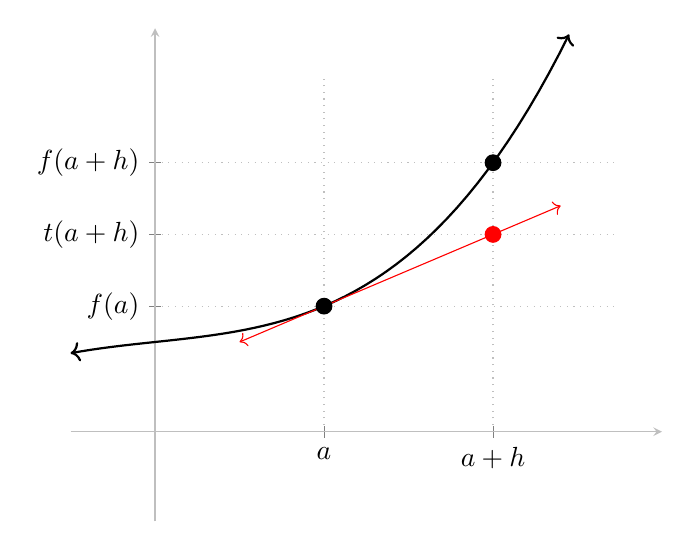
\begin{tikzpicture}
		\begin{axis}[
		xmin=-0.5,xmax=3,
		ymin=-0.5,ymax=2.25,
		ytick={0.7, 1.1, 1.5},
		xtick={1,2},
		xticklabels={$a$, $a+h$},
		yticklabels={$f(a)$, $t(a+h)$, $f(a+h)$},
		axis lines=middle,
		axis line style=lightgray,
		width=0.75\textwidth
		]
		\addplot[black,style=thick,<->] expression[domain=-0.5:2.45,samples=50]{(x*(x^2+1)+5)/10}; 
		
		
		\addplot[red,<->] expression[domain=0.5:2.4,samples=2]{0.4*x+0.3}; 
		
		
		\addplot[lightgray,dotted] expression[domain=0:2.75,samples=2]{0.7};
		\addplot[lightgray,dotted] expression[domain=0:2.75,samples=2]{1.1};
		\addplot[lightgray,dotted] expression[domain=0:2.75,samples=2]{1.5}; 
		\addplot +[mark=none,lightgray,dotted] coordinates {(1, 0) (1, 2)};
		\addplot +[mark=none,lightgray,dotted] coordinates {(2, 0) (2, 2)};
		
		\node[color=black,draw=black,circle,fill,inner sep=2pt] at (axis cs:1,0.7) {}; 
		\node[color=black,draw=black,circle,fill,inner sep=2pt] at (axis cs:2,1.5) {}; 
		\node[color=red,draw=red,circle,fill,inner sep=2pt] at (axis cs:2,1.1) {}; 
		\end{axis}
		\end{tikzpicture}
	\end{center}
	\caption{The graph of a function $f$ is depicted in black, and its tangent line $t$ at $a$ is depicted in red. Then the vertical distance $f(a+h)-f(a)$ is approximated by the vertical distance $t(a+h)-t(a)$. The ``rise'' $t(a+h)-t(a)$ can be computed as the slope times the ``run.'' In other words, $t(a+h)-t(a) = f'(a)h$. As $h$ gets smaller, this approximation of $f(a+h) - f(a)$ gets better.}  \label{figure-linear-approximation}
\end{figure}

Notice that the function $h \mapsto f'(a)h$ is a linear map $\R \to \R$, in the sense of linear algebra. The following result says that the function $h \mapsto f'(a)h$ is the \emph{only} linear map that is a good approximation\index{linear approximation} to $h \mapsto f(a+h)-f(a)$. The statement uses little-oh notation; if you have not seen this before, take a look at \cref{little-o-definition}.

\begin{proposition} \label{differential-unique-single}
	A function $f : S \to \R$ is differentiable at an interior point $a \in S$ if and only if there exists a linear map $\ell : \R \to \R$ such that
	\[ |f(a+h)-f(a) - \ell(h)| = o(|h|) \text{ as } h \to 0. \]
	Moreover, if there exists such a linear map $\ell$, then $\ell$ is uniquely determined: it must be given by \[ \ell(h) = f'(a)h \]
	for all $h \in \R$. 
\end{proposition}

\begin{proof}
	Let $\ell$ be a linear map $\ell(h) = ch$, where $c$ is some scalar. Observe that
	\[ \begin{aligned} \frac{|f(a+h)-f(a)-\ell(h)|}{|h|} &= \left| \frac{f(a+h)-f(a) - ch}{h} \right| \\
	&= \left| \frac{f(a+h)-f(a)}{h} - c \right|. \end{aligned} \]
	This leads us to the following sequence of ``if and only if'' statements. 
	\[ \begin{aligned} |f(a+h)-f(a)-\ell(h)| = o(|h|) &\iff \lim_{h \to 0} \frac{|f(a+h)-f(a)-\ell(h)|}{|h|} = 0 \\
	&\iff \lim_{h \to 0} \left| \frac{f(a+h)-f(a)}{h} - c \right| = 0 \\
	&\iff \lim_{h \to 0} \left( \frac{f(a+h)-f(a)}{h} - c \right) = 0 \\
	&\iff \lim_{h \to 0} \frac{f(a+h)-f(a)}{h} = c \end{aligned} \]
	The result follows. 
\end{proof}

\begin{definition}
	If $f : S \to \R$ is differentiable at an interior point $a \in S$, the \emph{differential} or the \emph{total derivative of $f$ at $a$}, denoted $df_a$, is the linear map $\R \to \R$ given by $df_a(h) = f'(a)h$. 
\end{definition}

Thus \cref{differential-unique-single} says that $df_a$ is the only ``good'' linear approximation to the function \[ h \mapsto f(a+h)-f(a). \] Since it is the only ``good'' linear approximation, it is also fair to say that it is the ``best'' linear approximation, whence the name of this section. The following is an important version of this same idea that comes up frequently in proofs. 

% TODO: add more here

\begin{remark}[Remainder function] \label{remainder-linear}
	Suppose $f : S \to \R$ is differentiable at an interior point $a \in S$. We define a remainder function\index{remainder} $r$ on sufficiently small values of $h$ by
	\[ r(h) = f(a+h) - f(a) - df_a(h). \]
	See \cref{figure-remainder-linear}. 
	\begin{figure}
		\begin{center}
			\begin{tikzpicture}
			\begin{axis}[
			xmin=-0.5,xmax=3,
			ymin=-0.5,ymax=2.25,
			ytick={0.7, 1.1, 1.5},
			xtick={1,2},
			xticklabels={$a$, $a+h$},
			yticklabels={$f(a)$, $f(a)+df_a(h)$, $f(a+h)$},
			axis lines=middle,
			axis line style=lightgray,
			width=\textwidth
			]
			\addplot[black,thick,<->] expression[domain=-0.5:2.45,samples=50]{(x*(x^2+1)+5)/10}; 
			
			
			\addplot[black,<->] expression[domain=0.1:2.4,samples=2]{0.4*x+0.3}; 
			
			
			\addplot[lightgray,dotted] expression[domain=0:2.75,samples=2]{0.7};
			\addplot[lightgray,dotted] expression[domain=0:2.75,samples=2]{1.1};
			\addplot[lightgray,dotted] expression[domain=0:2.75,samples=2]{1.5}; 
			\addplot +[mark=none,lightgray,dotted] coordinates {(1, 0) (1, 2)};
			\addplot +[mark=none,lightgray,dotted] coordinates {(2, 0) (2, 2)};
			
			
			\node[color=black,draw=black,circle,fill,inner sep=2pt] at (axis cs:1,0.7) {}; 
			\node[color=red,draw=red,circle,fill,inner sep=2pt] at (axis cs:2,1.5) {}; 
			\node[color=red,draw=red,circle,fill,inner sep=2pt] at (axis cs:2,1.1) {}; 
			
			
			\addplot +[mark=none,red,solid] coordinates {(2, 1.1) (2, 1.5)};
			\end{axis}
			\end{tikzpicture}
		\end{center}
		\caption{The thick black curve is the graph of a function $f$ and the thinner black line is its tangent line $f(a) + df_a$ are depicted in black. If $r$ is the remainder function, then $r(h)$ is the the vertical distance indicated in red above.}  \label{figure-remainder-linear}
	\end{figure}

	Notice that the $y$-value of the tangent line of $f$ at $a$ when $x = a+h$ is \[ f(a) + f'(a)h = f(a) + df_a(h), \]
	so $r(h)$ is what's left over after approximating $f$ by its tangent line (whence the name, ``remainder''). Notice that $r(0) = 0$. Moreover, $f$ is differentiable and therefore continuous at $a$ (cf. \cref{differentiable-implies-continuous-single}), so $r$ is also  continuous at 0. 
	
	Finally, the remainder function $r$ is ``small'' because $df_a$ is a ``good'' linear approximation of $f(a+h)-f(a)$. More precisely, we know from \cref{differential-unique-single} that $|r(h)| = o(|h|)$, which means that $r(h)/h \to 0$ as $h \to 0$. 
\end{remark} 

The following weak version of l'H\^opital's rule\index{lhopitals rule@L'H\^opital's rule} is an application of this idea. 
Note that this version of l'H\^opital's rule cannot be iterated (you cannot use it twice to evaluate $\lim_{x \to 0} (\sin x - x)/x^3$, for instance). In any case, in many cases it is often sufficient. 

\begin{exercise}[L'H\^opital's rule, weak version] \label{lhopital-weak}
	Suppose $f, g : S \to \R$ are differentiable at an interior point $a \in S$, that $f(a) = g(a) = 0$, and that $g'(a) \neq 0$. Show that
	\[ \lim_{x \to a} \frac{f(x)}{g(x)} = \frac{f'(a)}{g'(a)}. \]
	\begin{hint} 
		First show that, if $x = a+h$ and $r$ is the remainder function for $f$ defined in \cref{remainder-linear}, then
		\[ f(x) = f(a+h) = \left( f'(a) + \frac{r(h)}{h} \right)h. \]
	\end{hint}
\end{exercise} 

\section{Computing derivatives}

In this section, we'll prove some of the basic rules of differentiation that one normally encounters in an introductory calculus course. 

\subsection{Sum and scalar multiples rule}

The following results can be proved using either the definition of the derivative \ref{derivative-definition-single} or the ``best linear approximation'' characterization of \cref{differential-unique-single}. I strongly encourage you to try both methods for these exercises. 
When you use \cref{differential-unique-single}, you may find it useful to have done \cref{little-o-vector-space}. 

\begin{exercise}[Sum rule] \label{sum-rule-single} \index{sum rule}
	Prove that, if $f, g : S \to \R$ are both differentiable at an interior point $a \in S$, then $f + g$ is also differentiable at $a$ and \[ (f+g)'(a) = f'(a) + g'(a). \]
\end{exercise}

\begin{exercise}[Scalar multiples rule] \index{scalar multiples rule} \label{scalar-multiples-rule-single}
	Prove that, if $c$ is a constant and $f : S \to \R$ is differentiable at an interior point $a \in S$, then $cf$ is also differentiable at $a$ and \[ (cf)'(a) = c f'(a). \]
\end{exercise}

\begin{exercise}
	Suppose $f, g : S \to \R$ are functions and $f + g$ is differentiable at an interior point $a \in S$. Does it then follow that $f$ and $g$ are also differentiable at $a$? If so, prove it. If not, provide a counterexample. 
\end{exercise}

\subsection{Product and quotient rules}

\begin{proposition}[Product rule] \label{product-rule-single} \index{product rule}
	Suppose $f, g : S \to \R$ are both differentiable at $a \in S$. Then $fg$ is also differentiable at $a$ and 
	\[ (fg)'(a) = g(a) f'(a) + f(a)g'(a). \]
\end{proposition}

\begin{proof}
	The proof is a clever algebraic manipulation of difference quotients. The key trick is introducing a ``cross term'' of the form $f(a)g(a+h)$, and then cancelling it out by also introducing its negative. More precisely, for any sufficiently small real number $h$, we have 
	\[ \begin{aligned} \frac{(fg)(a+h)-(fg)(a)}{h} &= \frac{f(a+h)g(a+h) - f(a)g(a)}{h} \\ 
	&= \frac{f(a+h)g(a+h) {\color{blue}-f(a)g(a+h) + f(a)g(a+h)} - f(a)g(a)}{h} \\
	&= \frac{f(a+h)g(a+h) - f(a)g(a+h)}{h} + \frac{f(a)g(a+h) - f(a)g(a)}{h} \\
	&= g(a+h) \cdot \frac{f(a+h) - f(a)}{h} + f(a) \cdot \frac{g(a+h) - g(a)}{h}, \end{aligned} \]
	where the cross term and its negative is indicated in blue. 
	Taking the limit as $h \to 0$ yields the result. 
\end{proof}

\begin{exercise}
	Check your understanding of the above proof of the product rule. 
\begin{enumerate}[(a)]
	\item Could you have instead introduced a cross term of the form $f(a+h)g(a)$? If so, rewrite the proof using this cross term. If not, explain why not. 
	\item At what point is \cref{differentiable-implies-continuous-single} tacitly used in the above proof?
\end{enumerate}
\end{exercise}

\begin{exercise}
	 Reprove the scalar multiples rule (\cref{scalar-multiples-rule-single}) using the product rule. 
\end{exercise}

\begin{exercise}[Quotient rule] \label{quotient-rule-single} \index{quotient rule}
	Suppose $f, g : S \to \R$ are both differentiable at an interior point $a \in S$, and that $g(a) \neq 0$. Prove that $f/g$ is also differentiable at $a$ and 
	\[ (f/g)'(a) = \frac{g(a)f'(a) - f(a)g'(a)}{g(a)^2}. \] 
	\begin{hint} Observe that \[ \frac{(f/g)(a+h)-(f/g)(a)}{h} = \frac{\frac{f(a+h)}{g(a+h)} - \frac{f(a)}{g(a)} }{h}. \]
	Multiply both the numerator and denominator by $g(a+h)g(a)$ to clear the denominators inside the numerator, and then introduce the cross term $f(a)g(a)$. Be sure to notice at what point you use \cref{differentiable-implies-continuous-single}.
	\end{hint}
\end{exercise}

\begin{comment}
	Again, the proof is a clever algebraic manipulation of difference quotients! There are now two tricks: clearing denominators, and then introducing a cross term $f(a)g(a)$. 
	\[ \begin{aligned} \frac{(f/g)(a+h)-(f/g)(a)}{h} &= \frac{\frac{f(a+h)}{g(a+h)} - \frac{f(a)}{g(a)} }{h} \\ 
	&= \frac{g(a+h)g(a)}{g(a+h)g(a)} \cdot \frac{\frac{f(a+h)}{g(a+h)} - \frac{f(a)}{g(a)} }{h} \\
	&= \frac{1}{g(a+h)g(a)} \frac{f(a+h)g(a) - f(a)g(a+h)}{h} \\
	&= \frac{1}{g(a+h)g(a)} \frac{f(a+h)g(a) {\color{blue}- f(a)g(a) + f(a)g(a)} - f(a)g(a+h)}{h} \\ 
	&= \frac{1}{g(a+h)g(a)} \left( \frac{f(a+h)g(a) - f(a)g(a)}{h} + \frac{f(a)g(a) - f(a)g(a+h)}{h} \right) \\
	&= \frac{1}{g(a+h)g(a)} \left( \frac{f(a+h) - f(a)}{h} \cdot g(a) + f(a) \cdot \frac{g(a) - g(a+h)}{h} \right) \end{aligned} \]
\end{comment}

\begin{exercise}[Power rule for integer exponents] \label{power-rule-integer} \index{power rule}
	Extend the result of \cref{power-rule-positive} to arbitrary integer exponents. 
	\begin{hint} Use the quotient rule for negative integers. The exponent zero is a special but easy case (cf. \cref{constant-implies-derivative-zero-single}).  
	\end{hint}
\end{exercise}

\subsection{Chain rule} \label{chain-rule-single-section}

\begin{proposition}[Chain rule] \label{chain-rule-single} \index{chain rule}
	Suppose that $S$ and $T$ are both subsets of $\R$, that $f : S \to T$ is differentiable at an interior point $a$, that $f(a)$ is an interior point of $T$, and that $g : T \to \R$ is differentiable at $f(a)$. Then the composite $g \circ f : S \to \R$ is also differentiable at $a$, and 
	\[ (g \circ f)'(a) = g'(f(a))f'(a). \]
\end{proposition}

We will discuss two different (but similar) proofs of this important result. But first, here is an application. We will later prove a better version of this result (cf. \cref{inverse-function-theorem-single}). 

\begin{exercise}[Derivatives of inverses] \label{inverse-derivative} \index{inverse function}
	Suppose $f : S \to \R$ is differentiable at an interior point $a \in S$ and that $b = f(a)$ is an interior point of $f(S)$. Suppose further that $f$ is injective, so that the inverse function $f^{-1} : f(S) \to \R$ exists. Show that, if the inverse $f^{-1}$ is differentiable at $b$, then 
	\[ (f^{-1})'(b) = \frac{1}{f'(f^{-1}(b))}. \]
\end{exercise}

\subsubsection*{First proof}

The first proof uses the definition of the derivative \ref{derivative-definition-single}, but there is a subtle technicality involved; so, let us discuss it informally first before diving into the formal proof. The idea involved is again a clever rewriting of difference quotients. We introduce a cross term, which in this case is $f(a+h) - f(a)$. But this time we introduce this cross term ``multiplicatively'' rather than ``additively.'' More precsiely, we have
\[ \begin{aligned} \frac{(g \circ f)(a+h) - (g \circ f)(a)}{h} &= \frac{g(f(a+h)) - g(f(a))}{h} \\ &= \frac{g(f(a+h)) - g(f(a))}{f(a+h)-f(a)} \cdot \frac{f(a+h)-f(a)}{h}. \end{aligned} \]
The difference quotient on the right is precisely $f'(a)$. Thus, it would be sufficient to prove  
\begin{equation} \label{wrong-conjecture} \lim_{h \to 0} \frac{g(f(a+h)) - g(f(a))}{f(a+h)-f(a)} = g'(f(a)). \end{equation}
This formula looks an awful lot like the difference quotient that is used to define the derivative of $g$ at $f(a)$. In fact, since $f$ is continuous at $a$ by \cref{differentiable-implies-continuous-single}, we have $f(a+h) \approx f(a)+h$ for small values of $h$, which means that
\[ \frac{g(f(a+h)) - g(f(a))}{f(a+h)-f(a)} \approx \frac{g(f(a)+h) - g(f(a))}{f(a)+h-f(a)} = \frac{g(f(a)+h) - g(f(a))}{h} \]
for small values of $h$. Taking the limit as $h \to 0$ on the right-hand side yields precisely the definition of $g'(f(a))$, so \cref{wrong-conjecture} seems like a reasonable conjecture. 

The problem is that \cref{wrong-conjecture} isn't true. Issues arise when $f(a+h) = f(a)$ for arbitrarily small values of $h$, which leads to an infinite sequence of divisions by 0. More precisely, if, for every $\epsilon > 0$, there exists an $h$ such that $|h| < \epsilon$ and $f(a+h)=f(a)$, then 
\[ \frac{g(f(a+h)) - g(f(a))}{f(a+h)-f(a)} \]
cannot converge as $h \to 0$ at all. This kind of behavior, where $f$ keeps on repeating the value $f(a)$ arbitrarily close to $a$, is in fact possible, even when $f$ happens to be differentiable at $a$. This happens in the following example. 

\begin{example} \label{wrong-conjecture-counterexample}
	Let $f : \R \to \R$ be the function \[ f(x) = \begin{cases} x^2\sin(1/x) & \text{if } x \neq 0 \\ 0 & \text{if } x = 0. \end{cases} \] You will show in \cref{power-times-sine} that $f$ is in fact differentiable at 0. Set $h_k = 1/k\pi$. Then $h_k \to 0$ as $k \to \infty$, and $f(0 + h_k) = f(0)$ for all $k$. In other words, $f$ keeps on repeating the value 0 arbitrarily close to 0. 
\end{example}

We will get around the kind of issue that is described by the above example by carefully studying the expression
\begin{equation} \label{weird-difference-quotient} \frac{g(f(a+h)) - g(f(a))}{f(a+h)-f(a)}. \end{equation}
Observe that, when $f(a+h)\neq f(a)$, then this expression is precisely the difference quotient that calculates the slope of the secant line passing through $(f(a), g(f(a))$ and $(f(a+h), g(f(a+h))$. When $f(a+h) = f(a)$, this secant line doesn't make sense; but what does make sense is the tangent line! So we'll remove the undefinedness of expression \eqref{weird-difference-quotient} by extending it so that it takes the value $g'(f(a))$ whenever $f(a+h) = f(a)$. 

\begin{proof}[First proof of the chain rule]
	Consider the function $\Delta$ defined for small values of $h$ by \[ \Delta(h) = f(a+h)-f(a). \]
	See \cref{value-difference-chain-rule}. Then $\Delta(0) = 0$ and $\Delta$ is also continuous at 0 because $f$ is continuous at $a$, by \cref{differentiable-implies-continuous-single}. 
	
	\begin{figure}[t]
		\begin{center}
			\begin{tikzpicture}
			\begin{axis}[
			xmin=-0.5,xmax=3,
			ymin=-0.5,ymax=2.25,
			ytick={0.7, 1.5},
			xtick={1,2},
			xticklabels={$a$, $a+h$},
			yticklabels={$f(a)$,$f(a+h)$},
			axis lines=middle,
			axis line style=lightgray,
			width=0.75\textwidth
			]
			\addplot[black,style=thick,<->] expression[domain=-0.5:2.45,samples=50]{(x*(x^2+1)+5)/10}; 
			
			
			\addplot[lightgray,dotted] expression[domain=0:2.75,samples=2]{0.7};
			\addplot[lightgray,dotted] expression[domain=0:2.75,samples=2]{1.5}; 
			\addplot +[mark=none,lightgray,dotted] coordinates {(1, 0) (1, 2)};
			\addplot +[mark=none,lightgray,dotted] coordinates {(2, 0) (2, 2)};
			
			
			\node[color=black,draw=black,circle,fill,inner sep=2pt] at (axis cs:1,0.7) {}; 
			
			\node[color=red,draw=red,circle,fill,inner sep=2pt] at (axis cs:2,1.5) {}; 
			\node[color=red,draw=red,circle,fill,inner sep=2pt] at (axis cs:2,0.7) {}; 
			
			
			\addplot +[mark=none,gray,red,solid] coordinates {(2, 0.7) (2, 1.5)};
			\end{axis}
			\end{tikzpicture}
		\end{center}
		\caption{The graph of $f$ is depicted in black. The value of the function $\Delta$ on a small nonzero input value $h$ is the vertical distance depicted in red.}  \label{value-difference-chain-rule}
	\end{figure}

	Next, define a function $\sigma$ by the following.  
	\[ \sigma(k) = \begin{cases} \dfrac{g(f(a)+k) - g(f(a))}{k} & \text{if } k \neq 0 \\ g'(f(a)) & \text{if } k = 0 \end{cases} \]
	In other words, $\sigma$ is the function that, on some small nonzero input $k$, outputs the slope of the secant line connecting the two points $(f(a), g(f(a))$ and $(f(a)+k, g(f(a)+k))$. See \cref{slope-function-chain-rule}. It follows from the definition of the derivative of $g$ at $f(a)$ that the function $\sigma$ is continuous at 0. 
	
	\begin{figure}[t]
		\begin{center}
			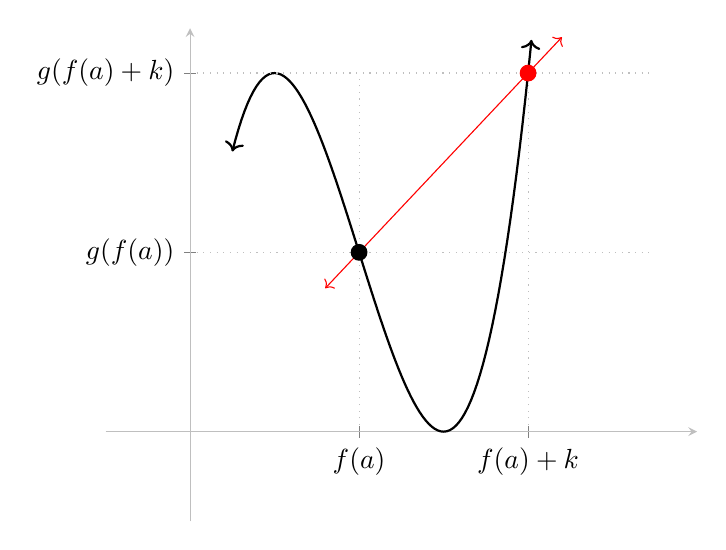
\begin{tikzpicture}
			\begin{axis}[
			xmin=-0.5,xmax=3,
			ymin=-0.5,ymax=2.25,
			ytick={1, 2},
			xtick={1,2},
			xticklabels={$f(a)$, $f(a)+k$},
			yticklabels={$g(f(a))$,$g(f(a)+k)$},
			axis lines=middle,
			axis line style=lightgray,
			width=0.75\textwidth
			]
			\addplot[black,style=thick,<->] expression[domain=0.25:2.02,samples=100]{4*x^3-12*x^2+9*x}; 
			
			
			\addplot[red,<->] expression[domain=0.8:2.2,samples=2]{(x-1)+1}; 
			
			
			\addplot[lightgray,dotted] expression[domain=0:2.75,samples=2]{1};
			\addplot[lightgray,dotted] expression[domain=0:2.75,samples=2]{2}; 
			\addplot +[mark=none,lightgray,dotted] coordinates {(1, 0) (1, 2)};
			\addplot +[mark=none,lightgray,dotted] coordinates {(2, 0) (2, 2)};
			
			\node[color=black,draw=black,circle,fill,inner sep=2pt] at (axis cs:1,1) {}; 
			
			\node[color=red,draw=red,circle,fill,inner sep=2pt] at (axis cs:2,2) {}; 
			\end{axis}
			\end{tikzpicture}
		\end{center}
		\caption{The graph of $g$ is depicted in black. The output of the function $\sigma$ on a small nonzero input value $k$ is the slope of the red secant line passing through the two points $(f(a), g(f(a))$ and $(f(a)+k, g(f(a)+k))$. }  \label{slope-function-chain-rule}
	\end{figure}
	
	
	You will verify in \cref{chain-rule-single-first-proof-details} below that
	\begin{equation} \label{alternative-to-multiplicative-cross-term} \frac{(g \circ f)(a+h) - (g \circ f)(a)}{h} = \sigma(\Delta(h)) \cdot \frac{f(a+h)-f(a)}{h} \end{equation}
	for all small values of $h$. Thus
	\[ \lim_{h \to 0} \frac{(g \circ f)(a+h) - (g \circ f)(a)}{h} = \lim_{h \to 0} \sigma (\epsilon(h)) \cdot \frac{f(a+h)-f(a)}{h} = g'(f(a)) f'(a) \]
	where we have used the continuity of $\epsilon$ and $\sigma$ and the definition of the derivative of $f$ at $a$ for the last step. This completes the proof. 
\end{proof}
	
\begin{exercise} \label{chain-rule-single-first-proof-details}
	Prove \cref{alternative-to-multiplicative-cross-term}. 
	\begin{hint} You might split up your proof of \cref{alternative-to-multiplicative-cross-term} into two cases: when $f(a+h) \neq f(a)$, and when $f(a+h) = f(a)$. 
	\end{hint}
\end{exercise}

\subsubsection*{Second proof}

Our second proof of the chain rule will use the ``best linear approximation'' interpretation of derivatives provided by \cref{differential-unique-single}. 

\begin{proof}[Second proof of the chain rule] \renewcommand{\qedsymbol}{}
	Note that, by definition of $dg_{f(a)}$ and $df_a$, we have 
	\[ dg_{f(a)}(df_a(h)) = g'(f(a))f'(a)h. \]
	Thus, by \cref{differential-unique-single}, it is sufficient to prove that
	\[ g(f(a+h))-g(f(a))-dg_{f(a)}(df_a(h)) = o(|h|) \text{ as } h \to 0. \]
	In other words, we want to prove that $g(f(a+h))-g(f(a))-dg_{f(a)}(df_a(h))$ is ``small.'' What we know is that the following remainder functions are ``small'' (cf. \cref{remainder-linear}).
	\[ \begin{aligned} 
	r(h) &= f(a+h)-f(a) - df_a(h) \\ 
	s(k) &= g(f(a)+k)-g(f(a))-dg_{f(a)}(k) \end{aligned} \]
	So the gist of the proof is to rewrite $g(f(a+h))-g(f(a))-dg_{f(a)}(df_a(h))$ in terms of $r$ and $s$, and then prove that it is ``small'' using the facts that $r$ and $s$ are ``small.''
	
	Rearranging the definition of $r(h)$ tells us that
	\begin{equation} \label{rearranged-definition-error} g(f(a+h)) = g(f(a) + df_a(h) + r(h)). \end{equation}
	Now note that the definition of $s(k)$ for $k = df_a(h) + r(h)$ says the following. 
	\[ \begin{aligned} s(df_a(h) + r(h)) &= g(f(a) + df_a(h) + r(h)) - g(f(a)) -dg_{f(a)}(df_a(h) + r(h)) \\
	g(f(a) + df_a(h) + r(h)) &= g(f(a)) + dg_{f(a)}(df_a(h) + r(h)) + s(df_a(h) + r(h)) \\
	&= g(f(a)) + dg_{f(a)}(df_a(h)) + dg_{f(a)}(r(h)) + s(df_a(h) + r(h))  \end{aligned} \]
	We used linearity of $dg_{f(a)}$ for the final step above. Combining this with \cref{rearranged-definition-error} show that
	\[ g(f(a+h)) - g(f(a)) - dg_{f(a)}(df_a(h)) = dg_{f(a)}(r(h)) + s(df_a(h)+r(h)). \]
	At this point, we've rewritten $g(f(a+h))-g(f(a))-dg_{f(a)}(df_a(h))$ in terms of $r$ and $s$. We'll now prove that the right-hand side is in fact ``small'', ie, that it is $o(|h|)$. Observe that \[ dg_{f(a)}(r(h)) = g'(f(a)) \cdot r(h), \] ie, $dg_{f(a)} \circ r$ is just a scalar multiple of $r$. We know that $r(h) = o(|h|)$ as $h \to 0$, so it follows that $dg_{f(a)}(r(h)) = o(|h|)$ also. So it is sufficient to prove that
	\[ s(df_a(h)+r(h)) = o(|h|). \]
	We've now hit the technical part, so let's hit pause. 
\end{proof}

To see why this is technical, and for essentially the same reasons as the previous proof, notice that we're trying to prove that
\[ \lim_{h \to 0} \frac{|s(df_a(h)+r(h)|)}{|h|} = 0.  \]
To prove this, it's tempting to introduce a multiplicative cross-term as follows. 
\[ \frac{|s(df_a(h)+r(h)|)}{|h|} = \frac{|s(df_a(h)+r(h)|)}{|df_a(h)+r(h)|} \cdot \frac{|df_a(h)+r(h)|}{|h|} \]
But notice that $df_a(h)+r(h) = f(a+h)-f(a)$ by definition of $r$, so this cross term is problematic for the same reasons as before! If $f(a+h) = f(a)$ for $h$ arbitrarily close to $0$, we have an infinite sequence of divisions by zeroes that causes problems. 

We'll deal with this problem in essentially the same way as before: namely, we extend the definition of 
\[\frac{|s(df_a(h)+r(h)|)}{|df_a(h)+r(h)|}\]
so that it is also defined when $f(a+h) = f(a)$. 

\begin{proof}[Second proof of the chain rule, continued]
	Define $\eta(k) = s(k)/k$ for nonzero $k$. Then extend $\eta$ by setting $\eta(0) = 0$. The fact that $s(k) = o(|k|)$ as $k \to 0$ implies that $\eta$ is continuous at 0. We now have \[ s(k) = \eta(k)k \]
	for all $k$. Applying this with $k = df_a(h) + r(h)$, we see that
	\[ \begin{aligned} \frac{|s(df_a(h)+r(h))|}{|h|} &= \frac{|\eta(df_a(h)+r(h))| \cdot |df_a(h)+r(h)|}{|h|} \\
	&\leq |\eta(df_a(h)+r(h))| \cdot \left( |f'(a)| + \frac{|r(h)|}{|h|} \right). \end{aligned} \]
	Since $r$ is continuous at 0 (cf. \cref{remainder-linear}), so is $df_a + r$. We have $(df_a + r)(0) = 0$, and we have just seen that $\eta$ is also continuous at $0$. Thus the composite $\eta \circ (df_a + r)$ is continuous at 0. Thus
	\[ \lim_{h \to 0} |\eta(df_a(h)+r(h))| \cdot \left( |f'(a)| + \frac{|r(h)|}{|h|} \right) = 0, \]
	where we have used the fact that $|r(h)| = o(|h|)$ to see that the parenthetical expression has a finite limit (namely, $|f'(a)|$). So, by the squeeze theorem, we can conclude that \[ |s(df_a(h)+r(h))| = o(|h|). \qedhere \]   
\end{proof}

Notice that in the first proof, the trick to overcoming the technicality was defining the function $\sigma$ at $k = 0$. In the second proof, the trick to overcoming the same technicality was defining $\eta$ at $k = 0$. These two tricks are really the same trick, as shown by the following.  

\begin{exercise}
	Prove that the function $\eta$ from the second proof and the function $\sigma$ from the first proof are related by the equation
	\[ \sigma(k) = g'(f(a)) + \eta(k). \]
\end{exercise}

\subsection{Interior extremum theorem}

We first recall the following definitions. 

\begin{definition} \index{extremum!local extremum} \index{extremum!local maximum} \index{extremum!local minimum} \index{extremum!absolute maximum} \index{extremum!absolute minimum} \index{extremum!absolute extremum}
	Supppose $X$ is a set, $f : X \to \R$ is a function, and $a \in X$. 
	\begin{itemize}
		\item $a$ is an \emph{absolute maximum}, or just \emph{maximum}, of $f$ if $f(x) \leq f(a)$ for all $x \in X$. 
		\item $a$ is a \emph{strict absolute maximum}, or just \emph{strict maximum} of $f$ if $f(x) < f(a)$ for all $x \in X \setminus\{a\}$. 
		\item $a$ is an \emph{absolute minimum}, or just \emph{minimum}, of $f$ if $f(x) \geq f(a)$ for all $x \in X$. 
		\item $a$ is a \emph{strict absolute minimum}, or just \emph{strict minimum} of $f$ if $f(x) > f(a)$ for all $x \in X \setminus\{a\}$. 
		\item $a$ is a \emph{absolute extremum}, or just \emph{extremum}, if it is either an absolute maximum or an absolute minimum. Similarly, $a$ is a \emph{strict absolute extremum}, or just \emph{strict extremum}, if it is either a strict absolute maximum or a strict absolute minimum. 
	\end{itemize}
	If $X$ is a metric space\footnotemark, we can also make the following definitions. 
	\begin{itemize}
		\item $a$ is a \emph{local maximum} of $f$ if there exists a neighborhood $U$ of $a$ in $X$ such that $f(x) \leq f(a)$ for all $x \in U$. 
		\item $a$ is a \emph{strict local maximum}, or just \emph{strict maximum} of $f$ if there exists a neighborhood $U$ of $a$ in $X$ such that $f(x) < f(a)$ for all $x \in U \setminus\{a\}$. 
		\item $a$ is a \emph{local minimum} of $f$ if there exists a neighborhood $U$ of $a$ in $X$ such that $f(x) \geq f(a)$ for all $x \in U$. 
		\item $a$ is a \emph{strict local minimum}, or just \emph{strict minimum} of $f$ if there exists a neighborhood $U$ of $a$ in $X$ such that $f(x) > f(a)$ for all $x \in U \setminus\{a\}$.
		\item $a$ is a \emph{local extremum} if it is either a local maximum or a local minimum. Similarly, $a$ is a \emph{strict local extremum} if it is either a strict local maximum or a strict local minimum. 
	\end{itemize}
\end{definition}

\footnotetext{For the definition of local extremums, $X$ could also be a topological space.}

The following is a key property of derivatives that you probably remember using frequently when you were first exposed to calculus. 

\begin{exercise}[Interior extremum theorem] \label{interior-extremum} \index{extremum!interior extremum theorem} \index{interior extremum theorem|see {extremum}}
	Suppose an interior point $a \in S$ is a local extremum of a function $f : S \to \R$. If $f$ is differentiable at $a$, prove that $f'(a) = 0$.
	\begin{hint} 
		Consider the following ``slope of secant'' function (which we've seen before, during the first proof of the chain rule in \cref{chain-rule-single-section}).
		\[ \sigma(h) = \begin{cases} \dfrac{f(a+h)-f(a)}{h} & \text{if } h \neq 0 \\ f'(a) & \text{if } h = 0 \end{cases} \]
		Since $f$ is differentiable at $x = a$, we know that $\sigma$ is continuous at $h = 0$. If $a$ is a local minimum, what can you say about the values of $\sigma$ for positive values of $h$? Negative values of $h$? Then consider the case when $a$ is a local maximum. 
	\end{hint}
\end{exercise}

But remember, the converse to the interior extremum theorem \ref{interior-extremum} is \emph{not} true. 

\begin{exercise} \label{interior-extremum-converse-false}
	Give an example of a function $f : \R \to \R$ such that $f'(0) = 0$, but $f$ does not have a local extremum at 0.\index{extremum!local extremum} 
\end{exercise}

\subsection{Non-rational functions} \label{non-rational}

Using the rules we've developed so far, we can differentiate any rational function (ie, a quotient of a polynomial by a polynomial). In this section, we will simply state some facts about differentiation of other types of functions one frequently encounters. We will prove most of these a bit later; we are stating them now so that we can discuss a richer repertoire of examples as we go along. We've already seen the need for a richer repertoire of examples in \cref{wrong-conjecture-counterexample}. 

\subsubsection*{Power rule}

First off, here is the most general statement of the power rule.

\begin{proposition}[Power rule for real exponents] \label{power-rule-general} \index{power rule}
	If $r$ is any real number and $f : (0, \infty) \to \R$ is the function $f(x) = x^r$, then $f'(x) = rx^{r-1}$ for all $x \in (0,\infty)$. 
\end{proposition}

We'll prove this for \emph{rational} exponents (ie, exponents that can be written as fractions of an integer over another integer) in \cref{power-rule-fractional}. We won't prove it in full generality, because that would require a long tangential discussion of what $x^r$ even means for irrational $r$. Actually, once we have a sufficiently rigorous definition of $x^r$ for irrational $r$, it turns out that \cref{power-rule-general} is actually a relatively straightforward \emph{consequence} of \cref{power-rule-fractional}. 

\subsubsection*{Exponential, sine, and cosine functions}

Next up, we have the exponential, sine, and cosine functions. These are usually defined by their power series\index{power series}, as follows. 
\begin{equation} \label{exp-sin-cos-power-series} \begin{aligned} \exp(x) &= \sum_{n = 0}^\infty \frac{x^n}{n!} \\
\cos(x) &= \sum_{n = 0}^\infty \frac{(-1)^n x^{2n}}{(2n)!} \\
\sin(x) &= \sum_{n = 0}^\infty \frac{(-1)^n x^{2n+1}}{(2n+1)!} \end{aligned} \end{equation}
All three of these have infinite radius of convergence (ie, they're defined for all real $x$). We'll prove that power series can be differentiated term-by-term in \cref{differentiating-power-series} inside their radius of convergences. This yields the following standard facts. 
\begin{enumerate}[(1)]
	\item If $f(x) = \exp(x)$, then $f'(x) = \exp(x)$. 
	\item If $f(x) = \sin(x)$, then $f'(x) = \cos(x)$. 
	\item If $f(x) = \cos(x)$, then $f'(x) = -\sin(x)$.
\end{enumerate} 

\begin{pedanticremark}
	Defining the exponential, sine, and cosine functions using power series is mathematically sound, but there are numerous facts about these functions that are not clear from the power series. For example, it's useful knowing that, if $e := \exp(1)$, then $\exp(x) = e^x$. This fact is not immediately clear from the power series definition; it requires some proof, and we won't prove it here, but you should feel free to use it. It's obviously also useful to know that sines and cosines have something to do with trigonometry. Again, this is not clear from the power series definition; it requires some proof, and we won't prove it, but you should feel free to use it. 
\end{pedanticremark}

% TODO: Geometric proof of the derivative of sines and cosines

\subsubsection*{Examples}

Let's now discuss some examples using these functions. The following two examples both involve the expression $\sin(1/x)$. As we will see, functions involving this expression exhibit a wild variety of interesting pathological behavior. 

\begin{exercise} \label{power-times-sine}
	\begin{enumerate}[(a)]
		\item Prove that the function \[ f(x) = \begin{cases} \sin(1/x) & \text{if } x \neq 0 \\ 0 & \text{if } x = 0 \end{cases} \]
		is discontinuous at 0. 
		
		\begin{hint}
			Show the following. 
			\[ \limsup_{x \to 0^{\pm}} \sin(1/x) = 1 \quad\quad \liminf_{x \to 0^{\pm}} \sin(1/x) = -1 \]
		\end{hint}
	
		\item Prove that the function \[ f(x) = \begin{cases} x\sin(1/x) & \text{if } x \neq 0 \\ 0 & \text{if } x = 0 \end{cases} \]
		is continuous, but that it is not differentiable at 0. 
		\item Prove that the function \[ f(x) = \begin{cases} x^2\sin(1/x) & \text{if } x \neq 0 \\ 0 & \text{if } x = 0 \end{cases} \]
		is differentiable, but that the derivative $f'$ is not continuous at 0.  
	\end{enumerate} 
\end{exercise}

The following example, again involving $\sin(1/x)$, illustrates a caveat to the interior extremum theorem \cref{interior-extremum}: even if $f$ has a local extremum at a point, it need not be that the derivative ``changes sign'' at that point.

\begin{exercise} \label{extremum-no-sign-change}
	Consider the function $f : \R \to \R$ given by 
	\[ f(x) = \begin{cases} x^4 \left( 2 + \sin(1/x) \right) & \text{if } x \neq 0 \\ 0 & \text{if } x = 0. \end{cases} \]
	\begin{enumerate}[(a)]
		\item Show that $f$ has an absolute minimum at 0.\index{extremum!absolute minimum} 
		\item Show that $f$ is differentiable and calculate the derivative $f'$. 
		\item Show that, on every open interval of the form $(a, 0)$ or $(0, b)$, the derivative $f'$ takes on both positive and negative values. 
	\end{enumerate}
\end{exercise}

\section{Differentiable functions} \label{single-differentiable}

In this section, we'll discuss some properties of functions which are differentiable everywhere on their domain. 

\begin{definition} \label{differentiable-open-domain-single} \index{differentiable} \index{derivative}
	Suppose $U$ is an open subset of $\R$. A function $f : U \to \R$ is \emph{differentiable} if it is differentiable at every point in $U$. The function $U \to \R$ given by $x \mapsto f'(x)$ is called the \emph{derivative} of $f$, and is denoted $f'$. 
\end{definition}

Every open subset of $\R$ is a countable disjoint union of open intervals\footnotemark\ (cf. \cite[theorem 6.17]{protter-morrey}), so the most important case of the above definition is when the domain happens to be an open interval. Occasionally, it's also useful to have some vocabulary for talking about functions on non-open intervals. Here is the ``correct'' definition for doing this.

\footnotetext{By the word \emph{interval}\index{interval}, we mean an uncountable connected subset of $\R$. This means that intervals can be open, closed, or half-open; and they can be bounded or unbounded. They cannot be just a single point.}

\begin{definition} \label{differentiable-any-domain-single}
	Suppose $S$ is any subset of $\R$ and $f : S \to \R$ is a function.
	\begin{itemize}
		\item We say that $f$ is \emph{differentiable on the interior} if $f$ is differentiable at every interior point of $S$ (ie, if the restriction of $f$ to the interior $S^\circ$ is differentiable in the sense of \cref{differentiable-open-domain-single}). The function $S^\circ \to \R$ given by $x \mapsto f'(x)$ is called the \emph{derivative} of $f$, and is denoted $f'$. 
		\item We say that $f$ is \emph{differentiable} if it is the restriction to $S$ of a differentiable function defined on an open neighborhood of $S$.  The function $S \to \R$ given by $x \mapsto f'(x)$ is called the \emph{derivative} of $f$, and is denoted $f'$. 
	\end{itemize} 
\end{definition}

\begin{pedanticremark}
	The reason these definitions are made the way they are is for precisely the same reasons discussed in the pedantic remark towards the end of \cref{slope-of-tangent-line}. 
\end{pedanticremark}

\subsection{Mean value theorem}

The mean value theorem \ref{mean-value-theorem}\index{mean value theorem} is an extremely important foundational result. You may remember seeing and ignoring it during your first calculus class; at least, that's what I did, and I think that's okay. Its importance largely derives from the fact that it comes up incredibly frequently when proving things formally about derivatives. 

\begin{theorem}[Mean value theorem]  \label{mean-value-theorem}
	Suppose $a < b$ and let $f : [a, b] \to \R$ be continuous and differentiable on the interior. Then there exists $c \in (a, b)$ such that
	\[ f'(c) = \frac{f(b) - f(a)}{b-a}. \]
\end{theorem}

Before proceeding, I encourage you to look at \cref{mean-value-theorem-picture} and ensure that you understand the geometric content of the statement. 

\begin{figure}
	\begin{center}
	\begin{tikzpicture}
	\begin{axis}[
	xmin=-0.1,xmax=2.5,
	ymin=-0.1,ymax=2,
	ytick={0.5, 1.5},
	xtick={0.5, 0.892375, 2},
	xticklabels={$a$, $c$, $b$},
	yticklabels={$f(a)$, $f(b)$},
	axis lines=middle,
	axis line style=lightgray,
	width=\textwidth
	]
	\addplot[black,thick,-] expression[domain=0.5:2,samples=50]{2/3*x+1/6 + 2*(x-0.5)*(x-1.5)*(x-2)}; 
	
	
	\addplot[black,<->] expression[domain=0.25:2.25,samples=2]{2/3*x+1/6}; 
	\addplot[red,<->] expression[domain=0.25:1.75,samples=2]{2/3*x+0.694821}; 
	
	
	\addplot[lightgray,dotted] expression[domain=0:2.75,samples=2]{0.5};
	\addplot[lightgray,dotted] expression[domain=0:2.75,samples=2]{1.5}; 
	\addplot +[mark=none,lightgray,dotted] coordinates {(0.5, 0) (0.5, 2)};
	\addplot +[mark=none,lightgray,dotted] coordinates {(2, 0) (2, 2)};
	
	
	\node[color=red,draw=red,circle,fill,inner sep=2pt] at (axis cs:0.892375,1.28974) {};
	\node[color=black,draw=black,circle,fill,inner sep=2pt] at (axis cs:0.5,0.5) {}; 
	\node[color=black,draw=black,circle,fill,inner sep=2pt] at (axis cs:2,1.5) {}; 
	\end{axis}
	\end{tikzpicture}
	\end{center}

	\caption{The mean value theorem \ref{mean-value-theorem} states that, if we draw a secant line connecting two points $(a,f(a))$ and $(b,f(b))$ on the graph of a differentiable function $f$, then that secant line must be parallel to the tangent line of $f$ at some point $c$ in between $a$ and $b$. The statement of the mean value theorem only asserts existence, not uniqueness; there could be multiple points $c$ at which this happens.} \label{mean-value-theorem-picture} 
\end{figure}

\begin{caution}
	Despite the similar sounding name, the mean value theorem is \emph{not} the same as the intermediate value theorem! The intermediate value theorem asserts that, if $f : [a,b] \to \R$ is continuous and $y$ is in between $f(a)$ and $f(b)$, then there exists $c \in (a,b)$ such that $f(c) = y$. The output of the intermediate value theorem is a point $c$ where the value of the function itself is some desired value (specifically, some value between $f(a)$ and $f(b)$), while the output of the mean value theorem is a point $c$ where the value of the \emph{derivative} is some desired value (specifically, the slope of the secant connecting $((a,f(a))$ and $(b,f(b))$. 
\end{caution}

Rolle's theorem \ref{rolles-theorem} is technically a special case of the mean value theorem, but the general case can be derived from this special case. 

\begin{exercise}[Rolle's theorem] \label{rolles-theorem} \index{mean value theorem!rolles theorem@Rolle's theorem} \index{rolles theorem@Rolle's theorem|see {mean value theorem}}
	Suppose $a < b$ and let $f : [a, b] \to \R$ be continuous and differentiable on the interior. If $f(a) = f(b) = 0$, prove that there exists $c \in (a, b)$ such that $f'(c) = 0$. 
	\begin{hint}
		Notice that any function must fall into at least one of the following three cases: (i) $f$ is constantly zero, (ii) $f$ takes on positive values somewhere on $[a, b]$, and (iii) $f$ takes on negative values somewhere on $[a, b]$. Deal with the first case using \cref{constant-implies-derivative-zero-single}, and the latter two cases using the extreme value theorem\footnotemark\ together with the interior extremum theorem \cref{interior-extremum}. 
	\end{hint}
\end{exercise}

\footnotetext{The \emph{extreme value theorem}\index{extremum!extreme value theorem} \index{extreme value theorem|see {extremum}} says that if $K$ is a compact metric space and $f : K \to \R$ is continuous, then $f$ achieves its global maximum and its global minimum somewhere on $K$ (cf. \cite[theorems 3.17 and 6.30]{protter-morrey}).}

\begin{exercise}
	Prove the mean value theorem. 
	\begin{hint} 
		Let $\ell$ be the secant line passing through $(a, f(a))$ and $(b, f(b))$. Then consider the function $g = f - \ell$. See \cref{subtracting-the-secant}. 
		Then $g(a) = g(b) = 0$, so we can apply Rolle's theorem \ref{rolles-theorem} to $g$.
	\end{hint} 
\end{exercise}

\begin{figure}
	\begin{center}
		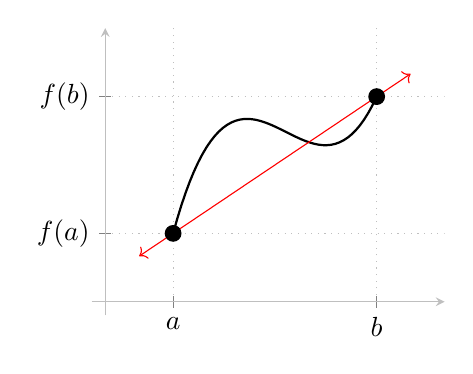
\begin{tikzpicture}
		\begin{axis}[
		xmin=-0.1,xmax=2.5,
		ymin=-0.1,ymax=2,
		ytick={0.5, 1.5},
		xtick={0.5,2},
		xticklabels={$a$, $b$},
		yticklabels={$f(a)$, $f(b)$},
		axis lines=middle,
		axis line style=lightgray,
		width=0.5\textwidth
		]
		\addplot[black,thick,-] expression[domain=0.5:2,samples=50]{2/3*x+1/6 + 2*(x-0.5)*(x-1.5)*(x-2)}; 
		
		
		\addplot[red,<->] expression[domain=0.25:2.25,samples=2]{2/3*x+1/6}; 
		
		
		\addplot[lightgray,dotted] expression[domain=0:2.75,samples=2]{0.5};
		\addplot[lightgray,dotted] expression[domain=0:2.75,samples=2]{1.5}; 
		\addplot +[mark=none,lightgray,dotted] coordinates {(0.5, 0) (0.5, 2)};
		\addplot +[mark=none,lightgray,dotted] coordinates {(2, 0) (2, 2)};
		
		
		\node[color=black,draw=black,circle,fill,inner sep=2pt] at (axis cs:0.5,0.5) {}; 
		\node[color=black,draw=black,circle,fill,inner sep=2pt] at (axis cs:2,1.5) {}; 
		\end{axis}
		\end{tikzpicture}\hspace{1cm}
		\begin{tikzpicture}
		\begin{axis}[
		xmin=-0.1,xmax=2.5,
		ymin=-1,ymax=1.1,
		ytick={0},
		xtick={0.5,2},
		xticklabels={$a$, $b$},
		yticklabels={},
		axis lines=middle,
		axis line style=lightgray,
		width=0.5\textwidth
		]
		\addplot[black,thick,-] expression[domain=0.5:2,samples=50]{2*(x-0.5)*(x-1.5)*(x-2)}; 
		
		\addplot[red,<->] expression[domain=0.25:2.25,samples=2]{0};
		
		\addplot +[mark=none,lightgray,dotted] coordinates {(0.5, -2) (0.5, 2)};
		\addplot +[mark=none,lightgray,dotted] coordinates {(2, -2) (2, 2)};
		
		\node[color=black,draw=black,circle,fill,inner sep=2pt] at (axis cs:0.5,0) {}; 
		\node[color=black,draw=black,circle,fill,inner sep=2pt] at (axis cs:2,0) {}; 
		\end{axis}
		\end{tikzpicture}
	\end{center}
	\caption{On the left is depicted the graph of a function $f$ and the secant line $\ell$. Subtracting $\ell$ from the picture on the left yields the picture on the right. }  \label{subtracting-the-secant}
\end{figure}

We can use the mean value theorem to prove the following ``if and only if upgrade'' of \cref{constant-implies-derivative-zero-single}. 

\begin{proposition} \label{constant-iff-derivative-zero-single}
	Suppose $I$ is an interval and that $f : I \to \R$ is continuous and differentiable on the interior. Then $f' = 0$ if and only if $f$ is constant\index{constant function}. 
\end{proposition}

\begin{proof}
	We showed in \cref{constant-implies-derivative-zero-single} that $f$ being constant implies $f' = 0$. Conversely, suppose we have $a < b$ in $I$. We want to show that $f(a) = f(b)$. Since $f$ is continuous and differentiable on the interior, the same is true on the compact subinterval $[a,b]$, so we can apply the mean value theorem on this interval. In other words, there exists a point $c \in (a,b)$ such that
	\[ \frac{f(b)-f(a)}{b-a} = f'(c). \]
	But $f'(c) = 0$ by assumption, so $f(a) = f(b)$. 
\end{proof}

Here are some more consequences. 

\begin{exercise} \label{bounded-derivative}
	Suppose $I$ is an interval and $f : I \to \R$ is continuous and differentiable on the interior. Let $M$ be a real number. Show that $|f'(x)| \leq M$ if and only if for all $x \in I$ if and only if \[ |f(b) - f(a)| \leq M|b-a| \] for all $a, b \in I$.
\end{exercise}

\begin{unimportantremark}
	Another way of stating the result of \cref{bounded-derivative} is that bounds on the derivative of $f$ are equivalent to \emph{Lipschitz constants} for $f$. In particular, having a bounded derivative implies \emph{Lipschitz continuity}. 
\end{unimportantremark}

\begin{exercise}[Fixed points] \label{fixed-points}
	Suppose $f : \R \to \R$ is a function. A \emph{fixed point} of $f$ is a point $\xi$ such that $f(\xi) = \xi$. 
	\begin{enumerate}[(a)]
		\item Suppose $f$ is differentiable and $f'(x) \neq 1$ for all $x \in \R$. Prove that $f$ has at most one fixed point. 
		\item Suppose $f$ is differentiable and there exists a constant $M < 1$ such that $|f'(x)| \leq M$ for all $x \in \R$.\footnote{Using the vocabulary of \cref{sup-norm}, this hypothesis can be rephrased by saying that $\|f'\|_\spn < 1$.}\ Show that $f$ has a unique fixed point.  
		
		\begin{hint}
			Pick any $x_0 \in \R$, and then inductively define $x_{n+1} = f(x_n)$ for all $n$. Prove inductively that $|x_{n+1} - x_n| \leq M^n|x_1 - x_0|$ for all $n$. Deduce that the sequence $x_0, x_1, x_2, \dotsc$ is Cauchy, and let $\xi = \lim x_n$. Then show that $\xi$ is a fixed point of $f$. 
		\end{hint}
	
		\item Suppose $f(x) = x + 1/(1 + \exp(x))$.
		Show that $f$ has no fixed points, and that $f$ is differentiable with $0 < f'(x) < 1$ for all $x \in \R$. Explain why this does not contradict part (b). 
	\end{enumerate}
\end{exercise}

\begin{exercise}[``Leveling off'' vs ``flattening out''] \label{leveling-off-vs-flattening-out}
	\begin{enumerate}[(a)]
		\item Suppose $f : (0, \infty) \to \R$ is differentiable and $f(x) \to 0$ as $x \to \infty$ (one might say informally that $f$ ``levels off'' near infinity). Show that, if 
		\[ \lim_{x \to \infty} f'(x) \]
		exists, then this limit must equal 0 (informally, one might say that that $f$ must ``flatten out'' near infinity).
		\item Let $f : (0, \infty) \to \R$ be defined by 
		\[ f(x) = \frac{\sin(x^2)}{x}. \]
		Show that ``levels off'' but does not ``flatten out'' near infinity.  
	\end{enumerate}
\end{exercise}

\begin{exercise}
	Suppose $f : \R \to \R$ is differentiable which ``flattens out'' near infinity; in other words, \[ \lim_{x \to \infty} f'(x) = 0. \] Let $g(x) = f(x+1) - f(x)$. Is it true that $g$ ``levels off'' near infinity (ie, that $g(x) \to 0$ as $x \to \infty$)? If so, prove it. If not, explain why not. 
\end{exercise}

\begin{exercise} \label{continuous-and-differentiable-except-at-point}
	Let $I$ be an open interval and $a \in I$. Suppose that $f : I \to \R$ is continuous, and suppose further that it is differentiable at every $x \in I$ except possibly at $a$. If \[ \lim_{x \to a} f'(x) \]
	exists, show that $f$ is also differentiable at $a$ and that $f'(a)$ is equal to this limit. 
\end{exercise}

\subsection{Monotonicity}

We begin by recalling the following definition. 

\begin{definition} \index{monotone} \index{monotone!increasing} \index{monotone!decreasing} \index{monotone!strictly monotone} \index{monotone!strictly increasing} \index{monotone!strictly decreasing} 
	Suppose $I$ is an interval and $f : I \to \R$ is a function.
	\begin{itemize}
		\item $f$ is \emph{increasing} $f(x) \leq f(y)$ for all $x < y$ in $I$. 
		\item $f$ is \emph{decreasing} $f(x) \geq f(y)$ for all $x < y$ in $I$.
		\item $f$ is \emph{strictly increasing} $f(x) < f(y)$ for all $x < y$ in $I$. 
		\item $f$ is \emph{strictly decreasing} $f(x) > f(y)$ for all $x < y$ in $I$. 
	\end{itemize}
Further, $f$ is \emph{monotone} if it is either increasing or decreasing, and \emph{strictly monotone} if it is either strictly increasing or strictly decreasing. 
\end{definition}

Here are some important properties of strictly monotone continuous functions.

\begin{exercise} \label{strictly-monotone-iff-injective}
	Suppose $I$ is an interval and $f : I \to \R$ is continuous. Prove that $f$ is injective if and only if $f$ is strictly monotone. 
\end{exercise}

\begin{exercise} \label{strictly-monotone-implies-open}
	Prove that, if $I$ is an open interval and $f : I \to \R$ is continuous and strictly monotone, then $f(I)$ is also an open interval. Conclude that $f$ is an open map\index{open!open map} (ie, that the image of any open subset of the domain is an open subset of $\R$).
	\begin{hint}
		Suppose $f$ is strictly increasing and $I = (a, b)$. Define $c = \lim_{x \to a^+} f(x)$ and $d = \lim_{x \to b^-} f(x)$ and use the intermediate value theorem to prove that $f(I) = (c, d)$. Then deal with the case when $f$ is strictly decreasing. 
	\end{hint}
\end{exercise}

The proofs of the following standard relationships between derivatives and monotonicity are similar to the proof of \cref{constant-iff-derivative-zero-single}.

\begin{exercise}[Derivatives and monotonicity] \label{monotone-derivative}
	Suppose $I$ is an interval and that $f : I \to \R$ is continuous and differentiable on the interior. 
	\begin{enumerate}[(a)]
		\item Prove that $f' \geq 0$ if and only if $f$ is increasing. 
		\item Prove that $f' \leq 0$ if and only if $f$ is decreasing.
	\end{enumerate}
	\begin{hint}
		You could basically repeat your proof of part (a) for part (b). Alternatively, notice that $f$ is decreasing if and only if $-f$ is increasing. 
	\end{hint}
\end{exercise}

\begin{solution}{\cref{monotone-derivative} part (a)}
	Suppose $f' \geq 0$ and $x < y$ in $I$. By the mean value theorem \ref{mean-value-theorem}, there exists $c$ between $x$ and $y$ such that 
	\[ \frac{f(y)-f(x)}{y-x} = f'(c) \geq 0. \]
	Since $y - x \geq 0$, this means that $f(y) \geq f(x)$, proving that $f$ is increasing. Conversely, suppose $f$ is increasing. Then for any $a \in I$ and $h > 0$, we have $f(a+h) \geq f(a)$, which means that 
	\[ \frac{f(a+h)-f(a)}{h} \geq 0 \]
	for all $h > 0$. Thus 
	\[ f'(a) = \lim_{h \to 0^+} \frac{f(a+h)-f(a)}{h} \geq 0, \]
	proving that $f' \geq 0$. 
\end{solution}

\begin{exercise}[Derivatives and strict monotonicity] \label{strictly-monotone-derivative}
	Suppose $I$ is an interval and that $f : I \to \R$ is continuous and differentiable on the interior. Prove the following. 
	\begin{enumerate}[(a)]
		\item If $f' > 0$, prove that $f$ is strictly increasing. 
		\item If $f' < 0$, prove that $f$ is strictly decreasing. 
		\item Unlike \cref{monotone-derivative}, the above two statements on strict monotonicity cannot be upgraded to ``if and only if'' statements. Give an example of a strictly increasing function $f : \R \to \R$ for which there exists some $a \in \R$ such that $f'(a) = 0$. 
		\item Notice that your proof of ``$f' \geq 0$ implies increasing'' from \cref{monotone-derivative} part (a) and ``$f' > 0$ implies strictly increasing'' from part (a) of this exercise are basically the same, except that all instances of ``$\geq$'' get replaced by ``$>$.'' Now inspect your proof of ``increasing implies $f' \geq 0$'' from \cref{monotone-derivative} part (a). Why can't you just replace all instances of ``$\geq$'' with ``$>$''?
	\end{enumerate} 
\end{exercise}

\begin{exercise}
	Suppose $f : \R \to \R$ is differentiable and there exists $M > 0$ such that $|f'(x)| \leq M$ for all $x \in \R$. Is it true that there must exist $\epsilon >  0$ such that the function $g : \R \to \R$ given by \[ g(x) = x + \epsilon f(x) \]
	is strictly increasing? If so, prove it. If not, explain why not. 
\end{exercise}

Again, there are pathologies involving monotonicity than can be exhibited by functions involving $\sin(1/x)$. Here is an example of a function whose derivative is positive at a single point, but it is not monotone near that point. 

\begin{exercise} \label{positive-not-monotone}
	Let $f : \R \to \R$ denote the function
	\[ f(x) = \begin{cases} x + 2x^2 \sin(1/x) & \text{if } x \neq 0 \\ 0 & \text{if } x = 0. \end{cases} \]
	\begin{enumerate}[(a)]
		\item Show that $f$ is differentiable and calculate $f'$. In particular, show that $f'(0) = 1$. 
		\item Show that $f$ is not monotone on any open interval containing 0.  
		\item Explain the ``2'' that shows up in the definition of $f$. Could it be replaced by 1 without changing the property of $f$ you proved in (b) above? Could it be replaced by 3? What is the set of all real numbers that it could be replaced with?
	\end{enumerate}
\end{exercise}

\subsection{Concavity}

Here is a word you probably recognize from calculus, but perhaps you haven't seen a formal definition. 

\begin{definition} \label{concave-up-definition}
	Suppose $I$ is an interval and $f : I \to \R$ is a function. We say that $f$ is \emph{concave up} (or \emph{convex}) if
	\[ \frac{f(y)-f(x)}{y-x} \leq \frac{f(z)-f(y)}{z-y} \]
	for all $x < y < z$ in $I$. 
	See \cref{concave-up-picture}. We say that $f$ is \emph{strictly concave up} (or \emph{strictly convex}) if 
	\[ \frac{f(y)-f(x)}{y-x} < \frac{f(z)-f(y)}{z-y} \]
	for all $x < y < z$ in $I$. 
	Similarly, we say that $f$ is \emph{concave down} (or just \emph{concave}) if
	\[ \frac{f(y)-f(x)}{y-x} \geq \frac{f(z)-f(y)}{z-y} \]
	for all $x < y < z$ in $I$, and we make an analogous definition for \emph{strictly concave down} (or just \emph{strictly concave}). 
\end{definition}

Notice that $f$ is (strictly) concave down if and only if $-f$ is (strictly) concave up. 

\begin{figure}[t]
	\begin{center}
		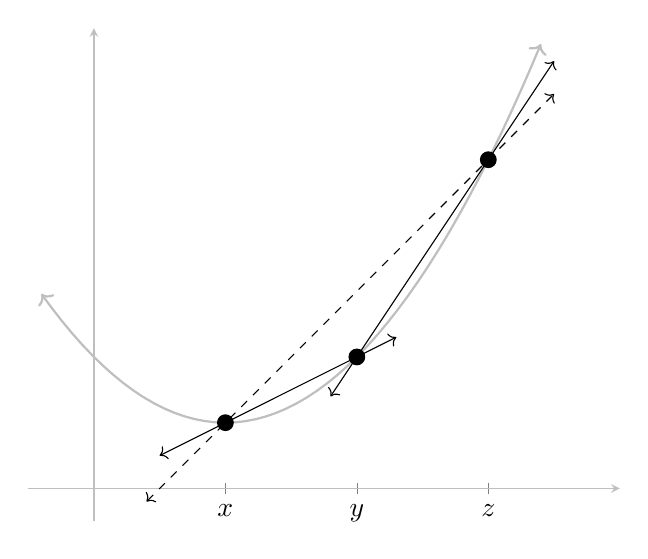
\begin{tikzpicture}
		\begin{axis}[
		xmin=-0.5,xmax=4,
		ymin=-0.5,ymax=7,
		xtick={1,2,3},
		ytick={0},
		xticklabels={$x$, $y$, $z$},
		yticklabels={},
		axis lines=middle,
		axis line style=lightgray,
		width=0.75\textwidth
		]
		\addplot[lightgray,style=thick,<->] expression[domain=-0.4:3.4,samples=50]{(x-1)^2+1}; 
		
		
		\addplot[black,<->] expression[domain=0.5:2.3,samples=2]{x}; 
		\addplot[black,<->] expression[domain=1.8:3.5,samples=2]{3*x-4};
		\addplot[black,dashed,<->] expression[domain=0.4:3.5,samples=2]{2*x-1};  
		
		\node[color=black,draw=black,circle,fill,inner sep=2pt] at (axis cs:1,1) {};
		\node[color=black,draw=black,circle,fill,inner sep=2pt] at (axis cs:2,2) {};
		\node[color=black,draw=black,circle,fill,inner sep=2pt] at (axis cs:3,5) {};
		
		\end{axis}
		\end{tikzpicture}
	\end{center}
	\caption{A function $f$ is defined to be \emph{concave up} in \cref{concave-up-definition} if the slope of the secant connecting $(x,f(x))$ and $(y,f(y))$ is less than or equal to the slope of the secant connecting $(y,f(y))$ and $(z,f(z))$ for all $x < y < z$. \Cref{concave-up-reformulation} says that, in this situation, the slope of the secant connecting $(x,f(x))$ and $(z,f(z))$ is in between the other two slopes. }  \label{concave-up-picture}
\end{figure}

\begin{lemma} \label{concave-up-reformulation}
	Suppose $I$ is an interval. A function $f : I \to \R$ is concave up if and only if 
	\[ \frac{f(y)-f(x)}{y-x} \leq \frac{f(z)-f(x)}{z-x} \leq \frac{f(z)-f(y)}{z-y} \]
	for all $x < y < z$ in $I$. 
\end{lemma}

\begin{proof}
	Clearly the double inequality in the statement of the lemma implies the single inequality in the definition. The proof of the converse is a rather unenlightening string of inequalities. 
	\begin{equation} \label{concave-up-reformulation-eqn1} \begin{aligned} \frac{f(y)-f(x)}{y-x} &\leq \frac{f(z)-f(y)}{z-y} \\
	(z-y)(f(y)-f(x)) &\leq (y-x)(f(z)-f(y)) \\
	zf(y) - zf(x) - yf(y) + yf(x) &\leq yf(z) - yf(y) - xf(z) +xf(y) \\
	zf(y) - zf(x) + yf(x) &\leq yf(z) - xf(z) + xf(y)
	\end{aligned} \end{equation}
	We'll take \cref{concave-up-reformulation-eqn1} and manipulate it to prove the two inequalities in the statement of the lemma. 
	
	First, if we take \cref{concave-up-reformulation-eqn1} and move the $yf(x)$ and $xf(y)$ terms to the opposite sides, and then add in $xf(x)$ to both sides, we see that 
	\[ \begin{aligned} 
	zf(y) - zf(x) - xf(y) &\leq yf(z) - yf(x) - xf(z) \\
	zf(y) - zf(x) - xf(y) + xf(x) &\leq yf(z) - yf(x) - xf(z) + xf(x) \\
	(z-x)(f(y)-f(x)) &\leq (y-x)(f(z)-f(x)) \\
	\frac{f(y)-f(x)}{y-x} &\leq \frac{f(z)-f(x)}{z-x},
	\end{aligned} \]
	which is one of the inequalities. On the other hand, if we move the $yf(z)$ and $zf(y)$ terms to the opposite sides in \cref{concave-up-reformulation-eqn1}, and then add in $zf(z)$ to both sides, we see that 
	\[ \begin{aligned} -zf(x) - yf(z) + yf(x) &\leq -zf(y) - xf(z) + xf(y) \\
	zf(z) -zf(x) - yf(z) + yf(x) &\leq zf(z) -zf(y) - xf(z) + xf(y) \\
	(z-y)(f(z)-f(x)) &\leq (z-x)(f(z)-f(y)) \\
	\frac{f(z)-f(x)}{z-x} &\leq \frac{f(z)-f(y)}{z-y}, \end{aligned} \]
	which is the other inequality. 
\end{proof}

\begin{unimportantremark}
	The proof above shows that either one of the two inequalities in the statement of \cref{concave-up-reformulation} implies that $f$ is concave up. 
\end{unimportantremark}

\begin{exercise}
	Suppose $f : [0, \infty) \to \R$ is concave up and that $f(0) = 0$. Show that the function $g : (0, \infty) \to \R$ defined by 
	\[ g(x) = \frac{f(x)}{x} \]
	is increasing. 
\end{exercise}

Here are some facts about how concavity relates to differentiation that you likely recognize from calculus. 

\begin{exercise}[Concavity and extremums] \label{concavity-extremums}
	Let $I$ be an open interval. Suppose $f : I \to \R$ is differentiable at a point $a \in I$ and $f'(a) = 0$. 
	\begin{enumerate}[(a)]
		\item If $f$ is concave up, show that $a$ is an absolute minimum of $f$. 
		\item If $f$ is concave down, show that $a$ is an absolute maximum of $f$. 
		\item If $f$ is strictly concave up, does it follow that $a$ is a strict absolute minimum of $f$? If so, prove it. If not, give a counterexample. 
	\end{enumerate} 
	\begin{hint}
		If $k < 0 < h$ and $f$ is concave up, then
		\[ \frac{f(a+k) - f(a)}{k} \leq \frac{f(a+h)-f(a)}{h}. \]
		Let $k \to 0^-$ to show that $a$ is a minimum on its right, and proceed similarly for the left. 
	\end{hint}
\end{exercise}

\begin{exercise}[Concavity and derivatives] \label{concavity-derivative}
	Suppose $I$ is an open interval and $f : I \to \R$ is differentiable. Prove the following. 
	\begin{enumerate}[(a)]
		\item $f$ is concave up if and only if $f'$ is increasing. 
		\item $f$ is concave down if and only if $f'$ is decreasing. 
		\item $f$ is strictly concave up if and only if $f'$ is strictly increasing. 
		\item $f$ is strictly concave down if and only if $f'$ is strictly decreasing. 
	\end{enumerate}
	\begin{hint}
		If $f'$ is (strictly) increasing, apply the mean value theorem \ref{mean-value-theorem} to prove that $f$ is (strictly) concave up. If $f$ is concave up, suppose we have $a < b$ in $I$. Let $x$ and $y$ be such that $a < x < y < b$. Explain why 
		\[ \frac{f(x)-f(a)}{x-a} \leq \frac{f(b)-f(y)}{b-y}, \]
		and then let $x \to a^+$ and $y \to b^-$. 
		The case when $f$ is \emph{strictly} concave up is a bit trickier (roughly because taking a limit can turn a $<$ into a  $\leq$), but one possible correct proof is a slight variant of the same idea. 
	\end{hint}
\end{exercise}

\subsection{Darboux's theorem \starred} \label{darboux-section}

Darboux's theorem asserts that derivatives are often ``close'' to being continuous, but in a weird way: they cannot have ``simple'' discontinuities, which means that when they are discontinuous at all, they are discontinuous in wild ways. 

\subsubsection*{Intermediate value property}

Before getting to the precise statement, we make the following definition. 

\begin{definition} \index{intermediate value property}
	Suppose $I$ is an interval and $f : I \to \R$ is a function. Then $f$ \emph{has the intermediate value property} if, for every $a < b$ in $I$ and every $y \in \R$ strictly between $f(a)$ and $f(b)$, there exists $x \in (a, b)$ such that $f(x) = y$.\footnote{Functions which have the intermediate value property are sometimes also called \emph{Darboux functions}.\index{Darboux function|see {intermediate value property}}} 
\end{definition}

Using this vocabulary, the intermediate value theorem\index{intermediate value theorem} asserts that every continuous function has the intermediate value property \cite[theorem 3.3]{protter-morrey}. Simple examples of discontinuous functions don't have the intermediate value property (cf. \cref{removable-jump-ivp} below). But, it turns out that some fairly bizarre discontinuous functions do have the intermediate value property (cf. \cref{discontinuous-ivp} below). 

\begin{exercise} \label{removable-jump-ivp}
	Let $I$ be an interval and $f : I \to \R$ a function. 
	\begin{enumerate}[(a)]
		\item Recall that $f$ has a \emph{removable discontinuity}\index{discontinuity!removable discontinuity} at a point $a \in I$ if
		\[ \lim_{x \to a} f(x) \]
		exists, but the value of this limit does not equal $f(a)$. Show that, if $f$ has a removable discontinuity, then $f$ does \emph{not} have the intermediate value property. 
		
		\item Recall that $f$ has a \emph{jump discontinuity}\index{discontinuity!jump discontinuity} at a point $a \in I$ if the two one-sided limits
		\[ \lim_{x \to a^-} f(x) \quad\text{ and }\quad \lim_{x \to a^+} f(x) \]
		both exist, but their values are not equal to each other. Show that, if $f$ has a jump discontinuity, then $f$ does \emph{not} have the intermediate value property.  
	\end{enumerate}
\end{exercise}

\begin{exercise} \label{discontinuous-ivp}
	Consider the function $f : \R \to \R$ defined by
	\[ f(x) = \begin{cases} \sin(1/x) & \text{if } x \neq 0 \\ 0 & \text{if } x = 0. \end{cases} \]
	We know from \cref{power-times-sine} that this function is discontinuous at 0. Show that it has the intermediate value property. \begin{hint} First show that for any interval $I$ containing 0, we have $f(I) = [-1,1]$. Then explain how this implies the intermediate value property. 
	\end{hint}
\end{exercise}

\subsubsection*{Statement of Darboux's theorem}

We know that the derivative $f'$ of a differentiable function $f$ need not be continuous (cf. \cref{power-times-sine}). Darboux's theorem asserts that, even though $f'$ might not be continuous, it must still have the intermediate value property! This means, for example, that derivatives cannot have removable or jump discontinuities (because, as we saw in \cref{removable-jump-ivp}, functions with these kinds of discontinuities do not have the intermediate value property). 

\begin{theorem}[Darboux] \label{darboux} \index{darbouxs theorem@Darboux's theorem}
	Suppose $I$ is an open interval and $f : I \to \R$ is differentiable. Then $f'$ has the intermediate value property.\index{intermediate value property} 
\end{theorem}

We noted earlier that the intermediate value theorem and the mean value theorem make similar but different assertions. Darboux's theorem now gets added to the fray! I encourage you to ensure that you understand how the statements of these three theorems differ (cf. \cref{ivt-mvt-darboux}).

\begin{table}
	\begin{center}
		{\scriptsize 
			\begin{tabular}{ p{0.17\textwidth} p{0.23\textwidth} p{0.23\textwidth} p{0.23\textwidth} } 
				\toprule[1pt]
				& Intermediate value theorem & Mean value theorem & Darboux's theorem \\ \cmidrule{2-4}
				If $f : [a, b] \to \R$ is... & continuous & continuous and differentiable on the interior & differentiable \\ \addlinespace[1em]
				& and $y$ is strictly in between $f(a)$ and $f(b)$ & & and $m$ is strictly in between $f'(a)$ and $f'(b)$ \\ \addlinespace[1em]
				then there exists $c$ in $(a,b)$ such that... & $f(c) = y$. & $f'(c) = \dfrac{f(b) - f(a)}{b-a}$. & $f'(c) = m$. \\ \bottomrule[1pt]
		\end{tabular}}
	\end{center}
	\caption{A tabular comparison of the statements of the intermediate value theorem, the mean value theorem, and Darboux's theorem.} \label{ivt-mvt-darboux}
\end{table}

Most functions that one encounters in life have continuous derivatives. In other words, most of the time, the fact that a derivative we're interested in has the intermediate value property would follow immediately from the intermediate value theorem. This makes Darboux's theorem not terribly important going forward, but it is a very interesting result nonetheless. Here are some applications. 

\begin{exercise} \label{nonzero-derivative-implies-strictly-monotone}
	Suppose $I$ is an open interval and $f : I \to \R$ is a differentiable function such that $f'(x) \neq 0$ for all $x \in I$. Show that $f$ is strictly monotone.
\end{exercise}

\begin{exercise}
	Let $I$ be an open interval. Suppose $f : I \to \R$ is a differentiable function and $a \in I$ is a point such that the one-sided limits
	\[ \lim_{x \to a^-} f'(x) \quad\text{ and }\quad \lim_{x \to a^+} f'(x) \]
	both exist (but are not assumed to be equal). Show that $f'$ is continuous at $a$ (in particular, this means that the above one-sided limits are forced to be equal). 
\end{exercise}

\subsubsection*{Proof of Darboux's theorem}

\begin{proof}[Proof of Darboux's theorem \ref{darboux}]
	Suppose $a < b$ are two elements of $I$ and $m$ is a real number strictly between $f'(a)$ and $f'(b)$. This means that either $f'(a) < m < f'(b)$ or $f'(a) > m > f'(b)$. Let us suppose that $f'(a) < m < f'(b)$ (the proof in the other case will be analogous). We want to show that there exists $c \in (a,b)$ such that $f'(c) = m$. We will prove this by considering an associated extreme value problem, and then applying the extreme value theorem\index{extremum!extreme value theorem}. 
	
	Specifically, consider the differentiable function $g : I \to \R$ defined by $g(x) = f(x) - mx$. See \cref{subtracting-a-line}. 
	Notice that \[ g'(x) = f'(x) - m, \] so $f'(c) = m$ if and only if $g'(c) = 0$. In other words, we would like to show that there exists $c \in (a, b)$ such that $g'(c) = 0$. By the extreme value theorem, we know that $g$ attains its minimum on the compact interval $[a,b]$ at some point $c \in [a,b]$. We claim that $c$ must be an interior point of $[a,b]$, and then interior extremum theorem \ref{interior-extremum} will imply that $g'(c) = 0$. 
	
	\begin{figure}[ht]
		\begin{center}
			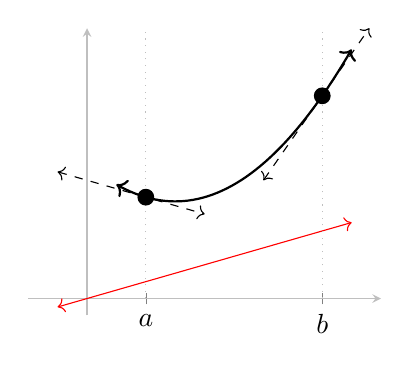
\begin{tikzpicture}
			\begin{axis}[
			xmin=-0.5,xmax=2.5,
			ymin=-0.25,ymax=4,
			xtick={0.5,2},
			ytick={0},
			xticklabels={$a$, $b$},
			yticklabels={},
			axis lines=middle,
			axis line style=lightgray,
			width=0.5\textwidth
			]
			\addplot[black,thick,<->] expression[domain=0.25:2.25,samples=50]{(x-1)^2+1 + x/2}; 
			
			
			\addplot[red,<->] expression[domain=-0.25:2.25,samples=2]{x/2}; 
			
			
			\addplot[dashed,<->] expression[domain=-0.25:1,samples=2]{-0.5*(x-0.5) + 1.5};
			\addplot[dashed,<->] expression[domain=1.5:2.4,samples=2]{2.5*(x-2) + 3}; 
			
			\addplot +[mark=none,lightgray,dotted] coordinates {(0.5, 0) (0.5, 4)};
			\addplot +[mark=none,lightgray,dotted] coordinates {(2, 0) (2, 4)};
			
			
			\node[color=black,draw=black,circle,fill,inner sep=2pt] at (axis cs:0.5,1.25+0.25) {}; 
			\node[color=black,draw=black,circle,fill,inner sep=2pt] at (axis cs:2,2+1) {}; 
			\end{axis}
			\end{tikzpicture}\hspace{1cm}
			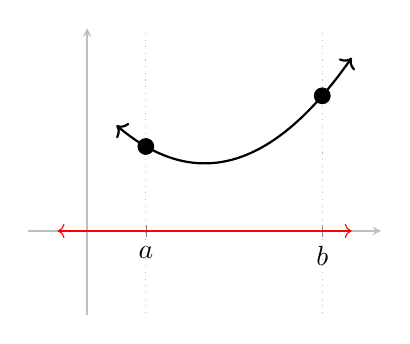
\begin{tikzpicture}
			\begin{axis}[
			xmin=-0.5,xmax=2.5,
			ymin=-1.25,ymax=3,
			ytick={0},
			xtick={0.5,2},
			xticklabels={$a$, $b$},
			yticklabels={},
			axis lines=middle,
			axis line style=lightgray,
			width=0.5\textwidth
			]
			\addplot[black,thick,<->] expression[domain=0.25:2.25,samples=50]{(x-1)^2+1}; 
			
			\addplot[red,<->] expression[domain=-0.25:2.25,samples=2]{0};
			
			\addplot +[mark=none,lightgray,dotted] coordinates {(0.5, -2) (0.5, 3)};
			\addplot +[mark=none,lightgray,dotted] coordinates {(2, -2) (2, 3)};
			
			\node[color=black,draw=black,circle,fill,inner sep=2pt] at (axis cs:0.5,1.25) {}; 
			\node[color=black,draw=black,circle,fill,inner sep=2pt] at (axis cs:2,2) {}; 
			\end{axis}
			\end{tikzpicture}
		\end{center}
		\caption{On the left is depicted the graph of a function $f$, the two tangent lines at $a$ and $b$, and the graph of the line $\ell(x) = mx$ for some $m$ in between $f'(a)$ and $f'(b)$. Subtracting $\ell$ from this picture yields the picture on the right.}  \label{subtracting-a-line}
	\end{figure}
	
	If $c = a$ were the minimum of $g$ on $[a,b]$, then we would have 
	\[ \frac{g(a+h)-g(a)}{h} > 0 \]
	for all sufficiently small positive values of $h$. This would mean that \[ f'(a) - m = g'(a) = \lim_{h \to 0^+} \frac{g(a+h)-g(a)}{h} \geq 0, \] which is a contradiction since $f'(a) < m$. Similarly, if $c = b$ were the minimum of $g$ on $[a,b]$, then we would have
	\[ \frac{g(b+h)-g(b)}{h} < 0 \]
	for all sufficiently small negative values of $h$. This would imply that 
	\[ f'(b) - m = g'(b) = \lim_{h \to 0^-} \frac{g(b+h)-g(b)}{h} \leq 0, \]
	which again is a contradiction since $m < f'(b)$. Thus we conclude that $c \in (a,b)$.  
	
	If instead we had $f'(a) > m > f'(b)$, we would define $c$ to be the point in $[a,b]$ where $g$ attains its \emph{maximum}. A similar argument then shows that $c$ must be an interior point. 
\end{proof}

\subsection{Inverse function theorem}

\begin{theorem} \label{inverse-function-theorem-single}
	Suppose that $I$ is an open interval, that $f : I \to \R$ is differentiable, and that $f'(x) \neq 0$ for all $x \in I$. Then $f$ is strictly monotone, the inverse function $f^{-1} : f(I) \to \R$ is differentiable, and 
	\[ (f^{-1})'(y) = \frac{1}{f'(f^{-1}(y))} \]
	for all $y \in f(I)$. 
\end{theorem}

\begin{proof}
	\Cref{nonzero-derivative-implies-strictly-monotone} tells us that $f$ is strictly monotone, and then \cref{strictly-monotone-implies-open} tells us that $f(I)$ is an open interval and that $f$ is open, ie, that $f^{-1}$ is continuous. To see that $f^{-1}$ is actually differentiable, fix $y \in f(I)$ and let $x = f^{-1}(y)$. For each $k$, define \[ h(k) = f^{-1}(y + k) - f^{-1}(y). \]
	Rearranging, this is equivalent the following. 
	\[ \begin{aligned} f^{-1}(y + k) &= f^{-1}(y) + h(k) \\
	f^{-1}(y + k) &= x + h(k) \\
	y + k &= f(x + h(k)) \\
	k &= f(x + h(k)) - y \\
	k &= f(x+h(k)) - f(x) \end{aligned} \]
	Thus, for any nonzero $k$, we have
	\[ \frac{f^{-1}(y + k) - f^{-1}(y)}{k} = \frac{h(k)}{k} = \frac{h(k)}{f(x + h(k)) - f(x)} = \frac{1}{ \left( \dfrac{f(x + h(k)) - f(x)}{h(k)} \right) } \]
	where for last step, we have used the fact that $h(k) \neq 0$ for all nonzero $k$ since $f^{-1}$ is injective. Since $f^{-1}$ is continuous at $y$, we have $h(k) \to 0$ as $k \to 0$. Thus the denominator on the far right above tends to $f'(x) = f'(f^{-1}(y))$ as $k \to 0$. Since the limit of the denominator is nonzero by assumption, the result follows from the quotient rule for limits. 
\end{proof}

\begin{exercise}[Power rule for fractional exponents] \label{power-rule-fractional} \index{power rule}
	Extend the result of \cref{power-rule-integer} to arbitrary rational exponents (ie, to exponents that can be written in the form $m/n$ where $m$ and $n$ are both integers). 
\end{exercise}

\begin{exercise} \label{derivative-log-proof}
	If $f(x) = \ln(x)$, prove that $f'(x) = 1/x$. You can use the facts that $\ln : (0, \infty) \to \R$ is the inverse of the exponential function, and that the exponential function is its own derivative. 
\end{exercise}

\subsection{Uniform limits \starred} \label{uniform-limit}

Derivatives interact somewhat strangely with limits. First off, here is an example to show that uniform limits of differentiable functions need not be differentiable. 

\begin{exercise}
	For any positive integer $n$, let $f_n : \R \to \R$ be the function
	\[ f_n(x) = \sqrt{x^2 + \frac{1}{n}}. \]
	\begin{enumerate}[(a)]
		\item Show that $f_n$ is differentiable. 
		\item Show that the $f_n$ converge uniformly to the absolute value function $f(x) = |x|$. 
		\item Show that the derivatives $f_n'$ converge pointwise but \emph{not} uniformly. 
	\end{enumerate}
\end{exercise}

In fact, even if a uniform limit of differentiable functions is differentiable, we cannot guarantee that the derivative of the limit is the limit of the derivatives; in fact, the derivatives need not converge at all.  

\begin{exercise}
	For any positive integer $n$, let $f_n : \R \to \R$ be the function 
	\[ f_n(x) = \frac{\sin(nx)}{n}. \]
	\begin{enumerate}[(a)]
		\item Show that $f_n$ is differentiable. 
		\item Show that the $f_n$ converge uniformly to 0. 
		\item Show that the derivatives $f_n'$ do \emph{not} converge pointwise. 
	\end{enumerate}
\end{exercise}

As suggested by part (c) of the previous two exercises, what we really need in order to have well-behaved interaction between limits and derivatives is uniform convergence \emph{of the derivatives}, rather than of the functions themselves. 

\begin{theorem} \label{differentiation-uniform-limit}
	Suppose $U$ is an open subset of $\R$ and $f_n : U \to \R$ is a differentiable function for each $n = 0, 1, \dotsc$ such that $\lim f_n = f$ pointwise. If the derivatives $f_n'$ converge uniformly on compact subsets of $U$, then $f$ is differentiable and $\lim f_n' = f'$. 
\end{theorem}

\begin{proof}
	Set $g = \lim f_n'$. Fix $a \in U$ and consider the following ``slope of secant'' functions (as in the first proof of the chain rule in \cref{chain-rule-single-section}). 
	\[ \begin{aligned} \sigma_n(h) &= \begin{cases} \dfrac{f_n(a+h) - f_n(a)}{h} & \text{if } h  \neq 0 \\ f_n'(a) & \text{if } h = 0 \end{cases} \\ 
	\sigma(h) &= \begin{cases} \dfrac{f(a+h) - f(a)}{h} & \text{if } h  \neq 0 \\ g(a) & \text{if } h = 0 \end{cases} \end{aligned} \]
	Continuity of $\sigma_n$ and $\sigma$ away from $h = 0$ is clear. At $h = 0$, we know that $\sigma_n$ is continuous because $f_n$ is differentiable at $a$. Note moreover that $\sigma_n$ converges pointwise to $\sigma$. 
	
	If we can show that $\sigma$ is continuous at $0$, then $f$ is differentiable at $a$ and $f'(a) = g(a) = \lim f_n'(a)$, which is what we ultimately want to prove. To show that $\sigma$ is continuous at 0, our strategy is to prove that $\sigma_n$ converges \emph{uniformly} to $\sigma$ on a compact interval $I$ containing 0 (not just pointwise, which we've already observed above). Then we can invoke the theorem guaranteeing that uniform limits of continuous functions are continuous (cf. \cite[theorem 9.13]{protter-morrey}) in order to conclude that $\sigma$ is continuous.
	
	Observe that for any pair of integers $m, n$ and any $h \in I \setminus \{0\}$, we have
	\[ \sigma_m(h) - \sigma_n(h) = \frac{(f_m(a+h) - f_n(a+h)) - (f_m(a) - f_n(a))}{h} = f_m'(\xi) - f_n'(\xi), \]
	where for the last step we have applied the mean value theorem to the function $f_m - f_n$ on the closed interval between $a$ and $a + h$ to find $\xi$ strictly between $a$ and $a + h$. Moreover, we have $\sigma_m(0) - \sigma_n(0) = f_m'(a) - f_n'(a)$. In other words, if we set $J = \{a + x : x \in I\}$, then for every $h \in I$, there exists $\xi \in J$ such that $\sigma_m(h) - \sigma_n(h) = f_m'(\xi) - f_n'(\xi)$, which implies that
	\[ \|\sigma_m - \sigma_n\|_{\spn, I} \leq \|f_m' - f_n'\|_{\spn, J}. \]
	Since the derivatives converge uniformly on the compact interval $J$, they are uniformly Cauchy. It follows from the above inequality that the $\sigma_n$ are also uniformly Cauchy, and therefore uniformly convergent. Since $\sigma$ is the pointwise limit of the $\sigma_n$, it must also be the uniform limit; in other words, we have now proved that $\sigma_n$ converges uniformly to $\sigma$, as we wanted. 
\end{proof}

\begin{unimportantremark}
	The hypotheses of this theorem can be made weaker by only assuming that the functions $f_n$ converge \emph{just at a single point} rather than pointwise on all of $U$, but one still needs to assume uniform convergence of the derivatives on compact subsets \cite[theorem 7.17]{rudin}. The idea of the proof of this generalization is similar to the proof above, but the flow of the argument gets obscured by more technical details. 
\end{unimportantremark}

% TODO: Convergence of the functions themselves is uniform.

This theorem lets us prove that we can differentiate power series term-by-term.

\begin{theorem} \label{differentiating-power-series}
	Suppose the power series $\sum_{n = 0}^\infty a_n x^n$
	has a nonzero radius of convergence $R$. Then the function $f : (-R, R) \to \R$ given by
	\[ f(x) = \sum_{n = 0}^\infty a_n x^n \]
	is differentiable and
	\[ f'(x) = \sum_{n = 0}^\infty na_n x^{n-1}. \]
	Moreover, the radius of convergence of the power series $\sum_{n = 0}^\infty na_n x^{n-1}$
	is also $R$. 
\end{theorem}

\begin{proof}
	Let 
	\[ f_n(x) = a_0 + a_1 x + \dotsb + a_n x^n \]
	be the sequence of the partial sums of the power series. Then clearly $\lim f_n = f$ pointwise. The conclusion of \cref{differentiating-power-series} would therefore follow by applying \cref{differentiation-uniform-limit} to the sequence $f_n$, provided we first show that $f_n'$ converges uniformly on compact subsets of $(-R, R)$. To prove this, it is sufficient to show that the radius of convergence of the power series 
	\[ \sum_{n = 0} na_n x^{n-1} \]
	is also $R$. Let $R'$ denote the radius of convergence of this power series; we want to show that $R' = R$. We also know that
	\[ \frac{1}{R} = \limsup_{n \to \infty} |a_n|^{1/n}.  \] 
	Observe that
	\[ \frac{1}{R'} = \limsup_{n \to \infty} |na_n|^{1/(n-1)} = \limsup_{n \to \infty} (|na_n|^{1/n})^{n/(n-1)}. \]
	Since $\lim n^{1/n} = 1$ and $\lim n/(n-1) = 1$, we conclude that $R = R'$. 
\end{proof}

\begin{exercise}
	Verify that, if the exponential, sine, and cosine functions are defined by their power series as in \cref{exp-sin-cos-power-series}, then their derivatives are calculated by the formulas we stated in \cref{non-rational}. 
\end{exercise}

\begin{comment}
%TODO: Bizarre differentiable functions \starred

This section is just for fun: we'll discuss many bizarre examples of differentiable functions. We'll start off with the following variant of a function we saw in \cref{power-times-sine}. 

\begin{exercise} \label{power-times-sine-truncated}
	Consider the function $f : \R \to \R$ defined as follows.
	\[ f(x) = \begin{cases} x^2 \sin(1/x) & \text{if } x >  0 \\ 0 & \text{if } x \leq 0 \end{cases} \]
	\begin{enumerate}[(a)]
		\item Show that $f$ is differentiable, and that
		\[ f'(x) = \begin{cases} 2x\sin(1/x) - \cos(1/x) & \text{if } x > 0 \\ 0 & \text{if } x \leq 0 \end{cases}. \]
		\item Show that $f'$ is continuous everywhere except at 0. 
		\item Show that $|f'(x)| \leq 3$ for all $x \leq 1$. 
	\end{enumerate}
\end{exercise}

\begin{example}
	Consider the function $h : \R \to \R$ defined as follows.
	\[ h(x) = \begin{cases} (1 - x^2)^2 \sin\left(\dfrac{1}{1 - x^2} \right) & \text{if } x \in (-1,1) \\ 0 & \text{otherwise} \end{cases} \]
	If $f : \R \to \R$ is the function from \cref{power-times-sine-truncated} and $g(x) = 1 - x^2$, observe that $h = f \circ g$. It follows from the chain rule \ref{chain-rule-single} that $h$ is differentiable and
	\[ h'(x) = f'(g(x)) g'(x). \]
	Since $f'$ is continuous everywhere except 0, we see that $h'$ is also continuous everywhere except when $g(x) = 0$, ie, when $x = \pm 1$. 
	
	We know that $h'(x) = 0$ on $(-\infty, -1]$ and $[1, \infty)$. On $(-1,1)$, observe that $0 < g(x) \leq 1$ and $|g'(x)| < 2$. Using the bound from the final part of \cref{power-times-sine-truncated}, 
	\[ |h'(x)| = |f'(g(x))||g'(x)| \leq 6. \]
	Thus $\|h'\|_\spn$ is finite. 
\end{example}

\begin{exercise} \label{derivative-discontinuous-two-points}
	For any $a < b$ in $\R$, construct a differentiable function $h : \R \to \R$ supported\footnotemark\ on $[a,b]$ such that $\|h'\|_{\spn} = 1$ and $h'$ is continuous everywhere except at $a$ and $b$. 
\end{exercise}

\footnotetext{Recall that the \emph{support}\index{support} of a function is the closure of the subset of its domain where it takes nonzero values.}

\begin{example}[Volterra]
	Let $F$ be a closed subset of $\R$ with empty interior. Then the complement of $F$ is an open subset of $\R$, so
	\[ \R \setminus F = \bigcup_{n = 0}^\infty (a_n, b_n) \]
	where the open intervals $(a_n, b_n)$ are all disjoint (cf. \cite[theorem 6.17]{protter-morrey}). Use \cref{derivative-discontinuous-two-points} to construct a differentiable function $h_n : \R \to \R$ supported on $[a_n, b_n]$ which is discontinuous at $a_n$ and $b_n$. Then consider the function
	\[ h(x) = \sum_{n = 0}^\infty \frac{h_n(x)}{2^n}. \] 
	This looks like an infinite series, but it's not. Every $x \in \R$ is either in $F$, in which case $h(x) = 0$, or there exists a unique integer $n$ such that $x \in (a_n, b_n)$, in which case $h(x) = h_n(x)/2^n$. Then $h$ is differentiable and $h'$ is discontinuous at all of the $a_0, b_0, a_1, b_1, \dotsc$. 
\end{example}
\end{comment}

\section{\texorpdfstring{$C^k$}{Ck} hierarchy} 

\subsection{Continuous differentiability}

We saw in \cref{darboux-section} that the derivative of a differentiable function is always ``close'' to being continuous, though in a slightly bizarre way. Insisting that the derivative actually be continuous is often useful for ruling out pathological behavior. 

\begin{definition}
	Suppose $U$ is an open subset of $\R$ and $f : U \to \R$ is differentiable. If the derivative $f' : U \to \R$ is also continuous, then $f$ is said to be \emph{continuously differentiable}.\index{continuously differentiable} 
\end{definition}

Here is an important ``reasonableness'' property of continuously differentiable functions. 

\begin{exercise} \label{critical-locus-closed-single}
	Show that, if $f : U \to \R$ is continuously differentiable, then the set
	\[ C = \{ x \in U : f'(x) = 0 \} \]
	is a closed subset of $U$. 
\end{exercise}

\Cref{critical-locus-closed-single} actually tells us that lots of strange pathological behavior is ruled out by insisting that the derivative is continuous. For example, we saw in \cref{positive-not-monotone} that $f(x) = x + 2x^2\sin(1/x)$ defined a differentiable function $f : \R \to \R$ such that $f'(0) \neq 0$, but which is not monotone on any interval containing that point. This is rather bizarre behavior, and it cannot happen with continuously differentiable functions. 

\begin{exercise} \label{nonzero-derivative-at-point-implies-monotone-in-neighborhood}
	Suppose $f : U \to \R$ is continuously differentiable, and $a \in U$ is a point such that $f'(a) \neq 0$. Use \cref{critical-locus-closed-single} to conclude that there exists an open interval containing $a$ on which $f$ is strictly monotone. 
\end{exercise}

To appreciate the following fact, it's worth noting the following: there exist \emph{non-constant} differentiable functions $f : U \to \R$ such that $f'(x) = 0$ for all $x \in U \cap \Q$! These extremely bizarre functions were first found by Pompeiu \cite{pompeiu}. This pathological behavior is also ruled out by insisting that the derivative be continuous. 

\begin{exercise} \label{critical-dense-implies-constant}
	Suppose $f : U \to \R$ is continuously differentiable. Use \cref{critical-locus-closed-single} to show that, if $f'(x) = 0$ for all $x \in U \cap \Q$, then $f$ is constant. 
\end{exercise}

Unfortunately, insisting that the derivative of a function be continuous does not rule out all possible bizarre behavior. For example, in \cref{extremum-no-sign-change}, we saw that $f(x) = x^4 \left( 2 + \sin(1/x) \right)$ defined a differentiable function $f$ with an absolute minimum at 0, but the derivative doesn't just simply ``change sign'' at 0. In fact, it turns out that function is also continuously differentiable (cf. \cref{extremum-no-sign-change-continued}), so merely insisting on continuous differentiability does not quite manage to rule out that kind of pathological behavior. However, as it turns out, the derivative of $f'$ (called the ``second derivative'' of $f$, and denoted $f''$), turns out \emph{not} to be continuous. 

\begin{exercise} \label{extremum-no-sign-change-continued}
	Let $f : \R \to \R$ be the function from \cref{extremum-no-sign-change}. Show that $f'$ is differentiable (so, in particular, $f$ is continuously differentiable), but that $f''$ is not continuous. 
\end{exercise}

This leads us to thinking about iterated derivatives. 

\subsection{\texorpdfstring{$C^k$}{Ck} functions}

\begin{definition} \label{ck-single} \index{ck@$C^k$}
	Let $U$ be an open subset of $\R$ and $f : U \to \R$ a function. We then define the following. 
	\begin{itemize}
		\item $f$ is said to be $C^0$ if it is continuous. 
		\item $f$ is said to be $C^1$ if it is continuously differentiable. 
		\item $f$ is said to be $C^2$ if it is differentiable and $f'$ is $C^1$. In this case, the derivative $(f')'$ of $f'$ is called the \emph{second derivative} of $f$, and is denoted either $f''$ or $f^{(2)}$. 
		\item $f$ is said to be $C^3$ if it is differentiable and $f'$ is $C^2$.  In this case, the second derivative $(f')''$ of $f'$ is called the \emph{third derivative} of $f$ and is denoted $f^{(3)}$. 
		\item $f$ is said to be $C^4$ if it is differentiable and $f'$ is $C^3$.  In this case, the third derivative $(f')^{(3)}$ of $f'$ is called the \emph{fourth derivative} of $f$ and is denoted $f^{(4)}$. 
	\end{itemize}
	Inductively, for any positive integer $k$, $f$ is said to be $C^k$ if it is differentiable and $f'$ is $C^{k-1}$.  In this case, the $(k-1)$st derivative $(f')^{(k-1)}$ of $f'$ is called the \emph{$k$th derivative} of $f$ and is denoted $f^{(k)}$.  
\end{definition}

First up, let's prove that all reasonable ways of combining functions in a particular differentiability class stays within that differentiability class. 

\begin{exercise} \label{ck-stable-sum-scalar-single}
	Prove that the set of all $C^k$ functions $U \to \R$ is a vector space. 
	\begin{hint}
		Induct on $k$. 
	\end{hint}
\end{exercise}

\begin{exercise} \label{ck-stable-product-single}
	\begin{enumerate}[(a)]
		\item Prove that the product of any two $C^k$ functions is also $C^k$. 
		\item If $f, g : U \to \R$ are $C^k$ functions, show that
		\[ (fg)^{(k)} = \sum_{i = 0}^k \binom{k}{i} f^{(i)} g^{(k-i)}. \]
	\end{enumerate}
\end{exercise}

\begin{exercise} \label{ck-stable-composite-single}
	Show that the composite of two $C^k$ functions is also $C^k$. \begin{hint} Induct on $k$. The base case $k = 0$ is clear. For the inductive step, use the chain rule \ref{chain-rule-single} and \cref{ck-stable-product-single}(a). \end{hint}
\end{exercise}

\begin{exercise} \label{ck-stable-reciprocal-single}
	Suppose $f : U \to \R$ is $C^k$ and $f(x) \neq 0$ for all $x \in U$. Show that $1/f$ is also $C^k$.
	\begin{hint}
		You might first show that the function $g(x) = 1/x$ is $C^k$ for all $k$. Then $1/f = g \circ f$, so you can apply \cref{ck-stable-composite-single}. 
	\end{hint}
\end{exercise}

\begin{proposition} \label{ck-stable-inversion-single}
	Suppose $I$ is an open interval, $f : I \to \R$ is injective, $C^k$ for some $k \geq 1$, and that $f'(x) \neq 0$ for all $x \in I$. Then $f^{-1} : f(I) \to U$ is also $C^k$. \index{inverse function}
\end{proposition}

\begin{proof}
	Since $f'$ is nonzero on $I$, we know from \cref{inverse-function-theorem-single} that $f^{-1}$ is differentiable and that
	\[ (f^{-1})'(a) = \frac{1}{f'(f^{-1}(a))}. \]
	In other words, $(f^{-1})'$ is the composite of three functions: $f^{-1}$, $f'$, and the function $x \mapsto 1/x$. 
	
	We will inductively prove that $f^{-1}$ is $C^r$ for all $0 \leq r \leq k$. Certainly $f^{-1}$ is $C^0$ (ie, continuous), since it is even differentiable, as we saw above. Inductively, suppose $f^{-1}$ is $C^r$ for some $0 \leq r < k$. We know that $f$ is $C^k$ and therefore $C^r$, and also that $x \mapsto 1/x$ is $C^r$ (cf. \cref{ck-stable-reciprocal-single}), so $(f^{-1})'$ is the composite of three $C^r$ functions. Thus \cref{ck-stable-composite-single} tells us that $(f^{-1})'$ is $C^r$, which shows that $f^{-1}$ is $C^{r+1}$. This completes the induction.  
\end{proof}

Observe that \cref{differentiable-implies-continuous-single} tells us that we have an infinite chain of implications
\[ \dotsb \implies C^3 \implies C^2 \implies C^1 \implies C^0. \]
The following shows that all of these implications are strict; in other words, for every $k$, there exists a $C^k$ function which is not $C^{k+1}$.

\begin{exercise}
	For any non-negative integer $k$, let 
	\[ f_k(x) = x^k|x|. \]
	See \cref{power-times-absolute-value-graphs}. Prove that $f_k$ is $C^k$, but the $(k+1)$st derivative $f^{(k+1)}$ does not exist. \begin{hint} First prove that $f_{k+1}' = (k+2)f_k$. \end{hint}
	
	\begin{figure}[ht]
		\begin{center}
			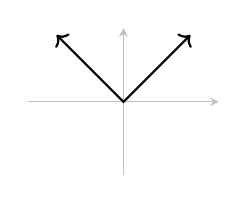
\begin{tikzpicture}
			\begin{axis}[
			xmin=-1.1,xmax=1.1,
			ymin=-1.1,ymax=1.1,
			xtick={0},
			ytick={0},
			axis lines=middle,
			axis line style=lightgray,
			width=0.33\textwidth,
			axis equal
			]
			\addplot[black,style=thick,<->] expression[domain=-1:1,samples=3]{abs(x)}; 
			
			\end{axis}
			\end{tikzpicture}
			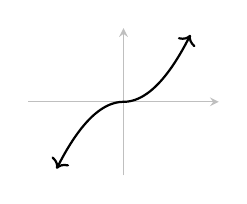
\begin{tikzpicture}
			\begin{axis}[
			xmin=-1.1,xmax=1.1,
			ymin=-1.1,ymax=1.1,
			xtick={0},
			ytick={0},
			axis lines=middle,
			axis line style=lightgray,
			width=0.33\textwidth,
			axis equal
			]
			\addplot[black,style=thick,<->] expression[domain=-1:1,samples=50]{x*abs(x)}; 
			
			\end{axis}
			\end{tikzpicture}
			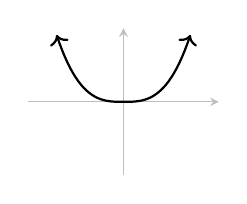
\begin{tikzpicture}
			\begin{axis}[
			xmin=-1.1,xmax=1.1,
			ymin=-1.1,ymax=1.1,
			xtick={0},
			ytick={0},
			axis lines=middle,
			axis line style=lightgray,
			width=0.33\textwidth,
			axis equal
			]
			\addplot[black,style=thick,<->] expression[domain=-1:1,samples=50]{x^2*abs(x)}; 
			
			\end{axis}
			\end{tikzpicture}
			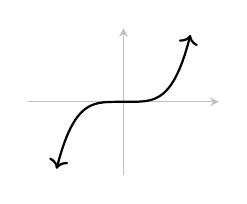
\begin{tikzpicture}
			\begin{axis}[
			xmin=-1.1,xmax=1.1,
			ymin=-1.1,ymax=1.1,
			xtick={0},
			ytick={0},
			axis lines=middle,
			axis line style=lightgray,
			width=0.33\textwidth,
			axis equal
			]
			\addplot[black,style=thick,<->] expression[domain=-1:1,samples=50]{x^3*abs(x)}; 
			
			\end{axis}
			\end{tikzpicture}
		\end{center}
		\caption{Graphs of the functions $f_k(x) = x^k|x|$ for $k = 0, 1, 2, 3$.} \label{power-times-absolute-value-graphs}
	\end{figure}
\end{exercise}

\begin{exercise}
	For any positive integer $k$, let $f_k : \R \to \R$ be the function given by
	\[ f_k(x) = \begin{cases} x^{k+1} \sin(1/x) &  \text{if } x \neq 0 \\ 0 & \text{if } x = 0. \end{cases} \]
	Show that the $k$th derivative $f^{(k)}$ exists, but it is not continuous. 
\end{exercise}

Here is a property of $C^2$ functions you likely recognize from calculus. 

\begin{exercise} \label{second-derivative-concavity}
	Suppose $I$ is an open interval and $f : I \to \R$ is $C^2$. 
	\begin{enumerate}[(a)]
		\item Show that $f$ is concave up if and only if $f'' \geq 0$.
		\item Show that $f$ is concave down if and only if $f'' \leq 0$.  
	\end{enumerate}
\end{exercise}

\begin{exercise} \label{second-derivative-strict-concavity}
	Suppose $I$ is an open interval and $f : I \to \R$ is $C^2$. 
	\begin{enumerate}[(a)]
		\item Show that, if $f'' > 0$, then $f$ is strictly concave up.
		\item Show that, if $f'' < 0$, then $f$ is strictly concave down. 
		\item Unlike \cref{second-derivative-concavity}, the above two statements cannot be upgraded to ``if and only if'' statements. Give an example of a strictly concave up function $f : \R \to  \R$ for which there exists some $a \in \R$ such that $f''(a) = 0$. 
	\end{enumerate}
\end{exercise}

\subsection{Taylor's theorem \starred}

Taylor's theorem gives us a way of approximating a $C^k$ function by a polynomial of at most degree $k$. When $k = 1$, the theorem says nothing more than \cref{differential-unique-single}.

\begin{theorem}[Taylor] \label{taylor-single}
	Suppose $I$ is an open interval, $f : I \to \R$ is $C^k$ for some non-negative integer $k$, and $a \in I$. Then there exists a unique polynomial $p_k$ at most $k$, called the \emph{degree $k$ Taylor polynomial of $f$ at $a$}, such that $|f(a+h) - p_k(h)| = o(|h|^k)$ as $h \to 0$. Moreover, we have
	\begin{equation} \label{taylor-polynomial-single} p_k(h) = f(a) + f'(a)h + \frac{f''(a)}{2!}h^2 + \frac{f^{(3)}(a)}{3!} h^3 + \dotsb + \frac{f^{(k)}(a)}{k!} h^k. \end{equation}
\end{theorem}

\begin{proof}
	Let $p_k(h)$ be defined as \cref{taylor-polynomial-single} and set $r(h) = f(a+h) - p_k(h)$. Observe that $r$ is $C^k$ by \cref{ck-stable-sum-scalar-single}. By direct calculation, we have $r^{(i)}(0) = 0$ for all $i = 0, 1, \dotsc, k$. If $k = 0$, then the fact that $|r(h)| = o(1)$ follows from the continuity (ie, $C^0$-ness) of $r$ and the fact that $r(0) = 0$; so we can assume for the rest of the proof that $k \geq 1$. 
	
	Suppose $h > 0$. By iterating the mean value theorem, we have
	\[ \begin{aligned} r(h) &= r(h) - r(0) \\
	&= r'(h_1)h = (r'(h_1) - r'(0))h \\
	&= r''(h_2)h_1 h = (r''(h_2) - r''(0))h_1 h \\
	&\enspace\vdots\\
	&= r^{(k-1)}(h_{k-1}) h_{k-2} h_{k-3} \dotsb h_2 h_1 h \end{aligned} \]
	where $0 < h_{k-1} < \dotsb < h_2 < h_1 < h$. This means that
	\[ \begin{aligned} \frac{|r(h)|}{|h|^k} &= \left| \frac{r^{(k-1)}(h_{k-1}) h_{k-2} \dotsb h_2 h_1 h}{h^k} \right| \\
	&\leq \left| \frac{r^{(k-1)}(h_{k-1}) h^{k-1}}{h^k} \right| \\
	&= \left| \frac{r^{(k-1)}(h_{k-1})}{h} \right| \\
	&\leq \left| \frac{r^{(k-1)}(h_{k-1})}{h_{k-1}} \right| \\
	&= \left| \frac{r^{(k-1)}(h_{k-1}) - r^{(k-1)}(0)}{h_{k-1}} \right|. \end{aligned}  \]
	Now as $h \to 0^+$, we also have that $h_{k-1} \to 0$, so this final expression tends to $r^{(k)}(0) = 0$. By the squeeze theorem, we conclude that 
	\[ \lim_{h \to 0^+} \frac{|r(h)|}{|h|^k} = 0. \]
	One argues similarly with $h < 0$ to prove that
	\[ \lim_{h \to 0^-} \frac{|r(h)|}{|h|^k} = 0. \]
	In this case, we have $h < h_1 < h_2 < \dotsb < h_{k-1} < 0$. This proves that $|r(h)| = o(|h|^k)$.
	
	To prove that $p_k$ is unique, suppose $q$ is any polynomial of degree at most $k$ such that $|f(a+h) -q(h)| = o(|h|^k)$. Then 
	\[ |p_k(h) - q(h)| \leq |f(a+h) - p_k(h)| + |f(a+h) - q(h)| \] 
	so \cref{little-o-vector-space,less-than-small-is-small} imply that $|p_k(h) -  q(h)| = o(|h|^k)$. But $p_k - q$ is a polynomial of degree at most $k$, and a nonzero polynomial of degree at most $k$ cannot be $o(|h|^k)$ as $h \to 0$. So we must have $p_k = q$.
\end{proof}

\begin{unimportantremark}
	It's worth remarking that Taylor's theorem does not use the fact that $f^{(k)}$ is continuous; it merely requires that $f^{(k)}$ exists, ie, that $f$ is \emph{$k$ times differentiable}. This is evident in the proof above. 
\end{unimportantremark}

The difference 
\[ r(h) = f(a+h) - p_k(h) \]
is often called a ``remainder,''\index{remainder} since it's what's left over after we approximate $f$ by its Taylor polynomial. When $k = 1$, this is precisely the remainder function we discussed in \cref{remainder-linear}.

\begin{exercise}[L'H\^opital's rule, less weak version] \label{lhopital-less-weak}
	Suppose $f, g : U \to \R$ are $C^k$ functions for some $k \geq 1$ and 
	\[ \begin{aligned} f(a) = f'(a) = \dotsb = f^{(k-1)}(a) = 0 \\
	g(a) = g'(a) = \dotsb = g^{(k-1)}(a) = 0 \end{aligned} \]
	and $g^{(k)}(a) \neq 0$. Prove that 
	\[ \lim_{x \to a} \frac{f(x)}{g(x)} = \frac{f^{(k)}(a)}{g^{(k)}(a)}. \]
	\begin{hint}
		Mimic the proof of \cref{lhopital-weak}, but now use $r(h) = f(a+h) - p_k(h)$ instead of $r(h) = f(a+h) - p_1(h)$. 
	\end{hint}
\end{exercise}

\begin{exercise}
	Suppose $f : U \to \R$ is $C^2$ and $a \in U$ is a point such that $f'(a) = 0$. 
	\begin{enumerate}[(a)]
		\item Show that, if $f''(a) > 0$, then $a$ is a strict local minimum of $f$, and that if $f''(a) < 0$, then $a$ is a strict local maximum of $f$. 
		\begin{hint}
			You can do this using \cref{concavity-extremums,second-derivative-strict-concavity}. Alternatively, you can do it using Taylor's theorem \ref{taylor-single}. Try both methods. It's the Taylor's theorem method that will be more helpful for part (c) below. You may also notice that the first method really requires that $f$ be $C^2$, while the Taylor's theorem method only requires that $f$ be twice differentiable. 
		\end{hint}
	
		\item Give examples to show that, if $f''(a) = 0$, then the test from part (a) is entirely inconclusive: $a$ could be a strict local extremum (of either type), a non-strict local extremum (of either type), or not a local extremum at all. 
		
		\item Suppose $f$ is $C^k$ for some $k \geq 2$, that 
		\[ f'(a) = f^{(2)} = \dotsb = f^{(k-1)}(a) = 0 \]
		and that $f^{(k)}(a) \neq 0$. Formulate and prove a rule that uses the sign of $f^{(k)}(a)$ and/or the parity of $k$ to determine whether or not $a$ is a local extremum, and if it is a local extremum, what kind of local extremum it is. 
	\end{enumerate}
\end{exercise}

We now return to our discussion of the pathology exhibited by the function $f(x) = x^4 \left( 2 + \sin(1/x) \right)$ from \cref{extremum-no-sign-change,extremum-no-sign-change-continued}, which has the strange property that $f'(0) = 0$ but $f$ is not monotone on any interval to the left or to the right of 0. Such pathologies cannot occur if the function eventually has a nonzero derivative. 

% We prepare for this discussion with the following lemma. 
\begin{comment}
\begin{lemma} \label{eventual-nonvanishing-derivative}
	Suppose $I$ is an open interval, $f : I \to \R$ is $C^k$ for some positive integer $k$, that 
	\[ f(a) = f'(a) = f^{(2)}(a) = \dotsb = f^{(k-1)}(a) = 0, \] and that $f^{(k)}(a) > 0$. Then there exists an $\epsilon > 0$ such that $f$ is positive on $(a, a+\epsilon)$, and on $(a-\epsilon, a)$, $f$ is positive if $k$ is even and negative if $k$ is odd. Moreover, if $f^{(k)}(a) < 0$, then all instances of ``positive'' in the conclusion get replaced by ``negative'' and vice versa. 
\end{lemma}

\begin{proof}
	Let us suppose that $f^{(k)}(a) > 0$. By Taylor's theorem \ref{taylor-single}, we see that
	\[ f(a+h) = \frac{f^{(k)}(a)}{k!} h^k + r(h) \]
	where $|r(h)| = o(|h|^k)$ as $h \to 0$. Dividing through by $h^k$, we see that 
	\[ \frac{f(a+h)}{h^k} = \frac{f^{(k)}(a)}{k!} + \frac{r(h)}{h^k}. \]
	Since $f^{(k)}(a) > 0$, we also have $f^{(k)}(a)/k! > 0$. Since $\lim_{h \to 0} |r(h)/h^k| = 0$, there exists $\epsilon > 0$ such that $|r(h)/h^k| < f^{(k)}(a)/k!$ for all $|h| < \epsilon$. Then, if $0 < |h| < \epsilon$, we have
	\[ \frac{f(a+h)}{h^k} = \frac{f^{(k)}(a)}{k!} + \frac{r(h)}{h^k} > 0. \]
	Now note that if $k$ is even, then $h^k$ is always positive, so the lemma follows. On the other hand, if $k$ is odd, then $h^k$ is positive for positive $h$ and negative for negative $h$, and again the lemma follows. The proof when $f^{(k)}(a) < 0$ is similar. 
\end{proof}
\end{comment}

\begin{exercise} \label{extremum-sign-change}
	Suppose $f$ is $C^k$ for some $k \geq 2$, that
	\[ f'(a) = f^{(2)}(a) = \dotsb = f^{(k-1)}(a) = 0 \] and $f^{(k)}(a) \neq 0$. Prove that there exists an $\epsilon > 0$ such that $f$ is strictly monotone on $(a-\epsilon, a)$ and on $(a, a+\epsilon)$. 
\end{exercise}

\begin{example} \label{extremum-no-sign-change-final}
	Let $f : \R \to \R$ be the function $f(x) = x^4(2 + \sin(1/x))$ of \cref{extremum-no-sign-change,extremum-no-sign-change-continued}. Then $f$ is twice differentiable and $f'(0) = f''(0) = 0$, but it is not thrice differentiable at 0. In other words, it doesn't eventually have a nonzero derivative at 0, so we're not able to apply \cref{extremum-sign-change}. 
\end{example}

It turns out that if $f$ is $C^{k+1}$, we can use the mean value theorem to express the remainder in terms of the $(k+1)$st derivative. 

\begin{theorem}[Taylor's theorem with remainder, Lagrange form] \label{taylor-single-remainder-lagrange}
	Suppose $I$ is an open interval, $f : I \to \R$ is $C^{k+1}$ for some non-negative integer $k$ and $a \in I$. Then for any $h$ such that $a+h \in I$, there exists $\xi$ between $a$ and $a+h$ such that 
	\[ f(a+h) - p_k(h) = \frac{f^{(k+1)}(\xi)}{(k+1)!}h^{k+1}, \]
	where $p_k$ is the degree $k$ Taylor polynomial of $f$ at $a$. 
\end{theorem}

\begin{proof}
	When $k = 0$, we have $p_0(h) = f(a)$ and the statement follows immediately from the mean value theorem \ref{mean-value-theorem}. So we can assume that $k \geq 1$. Let $r(h) = f(a+h) - p_k(h)$. Fix $h > 0$ and consider the function
	\[ g(t) = r(t) - \frac{r(h)}{h^{k+1}} t^{k+1}.  \]
	Plugging in $t = h$, we see that $g(h) = 0$. As we noted in the proof of Taylor's theorem \ref{taylor}, we have $r^{(i)}(0) = 0$ for $i = 0, 1, \dotsc, k$, from which it follows that $g^{(i)}(0) = 0$ for $i = 0, 1, \dotsc, k$. Moreover, we have \[ g^{(k+1)}(t) = f^{(k+1)}(t) - \frac{(k+1)!r(h)}{h^{k+1}},  \]
	because $p_k$ is a polynomial of degree at most $k$, which means that its $(k+1)$st derivative vanishes. 
	
	Since $g(0) = g(h) = 0$, Rolle's theorem \ref{rolles-theorem} tells us that there exists $h_1$ between $0$ and $h$ such that $g'(h_1) = 0$. Since $g'(0) = g'(h_1) = 0$, Rolle's theorem again gives us $h_2$ between $0$ and $h_2$ such that $g^{(2)}(h_2) = 0$. Inductively, we find a sequence $0 < h_{k+1} < h_k < h_{k-1} < \dotsb < h_1 < h$ such that $g^{(i)}(h_i) = 0$ for all $i = 0, \dotsc, k, k+1$. Letting $\xi = h_{k+1}$, we find that 
	\[ 0 = g^{(k+1)}(\xi) = f^{(k+1)}(\xi) - \frac{(k+1)!r(h)}{h^{k+1}}, \]
	and rearranging this equation yields precisely
	\[ f(a+h) - p_k(h) = r(h) = \frac{f^{(k+1)}(\xi)}{(k+1)!}h^{k+1}. \]
	The proof when $h < 0$ is analogous. 
\end{proof}

\subsection{Smooth functions} \label{smooth-single}

Insisting that a function be $C^k$ for larger and larger values of $k$ rules out more and more pathological behavior. This suggests the following. 

\begin{definition} \index{smooth} \index{Cinfinity@$C^\infty$|see {smooth}} \index{infinitely differentiable|see {smooth}}
	A function $f : U \to \R$ is said to be $C^\infty$, or \emph{infinitely differentiable}, or \emph{smooth}, if it is $C^k$ for all $k$. 
\end{definition}

It's a little annoying that there are three different words that all mean the same thing, but that's just how it is; all three are commonly used in the mathematical literature, so it's best to get used to all of them. We'll usually use the word ``smooth.'' 

It follows immediately from \cref{ck-stable-sum-scalar-single,ck-stable-product-single,ck-stable-reciprocal-single,ck-stable-composite-single,ck-stable-inversion-single} that sums, scalar multiples, products, reciprocals, composites, and inverses of smooth functions are also smooth. 

The class of smooth functions is very well-behaved. On the one hand, as we have already seen, smoothness rules out lots of pathological behavior. For example, functions like \cref{positive-not-monotone} are not smooth, and in fact, if the derivative of a smooth function $f$ is nonzero at a single point, then $f$ must be strictly monotone in a neighborhood of that point (cf. \cref{nonzero-derivative-at-point-implies-monotone-in-neighborhood}). We've also seen that functions like the one from \cref{extremum-no-sign-change,extremum-no-sign-change,extremum-no-sign-change-final} are not smooth, and that if $f$ is smooth and $a$ is a local extremum and eventually $f$ has a nonzero derivative at $a$, then in fact the derivative of $f$ must ``change sign'' at $a$ (cf. \cref{extremum-sign-change}). 

On the other hand, the class of smooth functions is not overly restrictive. There is a vast array of smooth functions, and we can tailor smooth functions to almost arbitrary specifications. 

\subsubsection*{Diffeomorphisms}

Our first example of this principle is the following smooth bijection $(-1,1) \to \R$ whose inverse is also smooth. A smooth bijection with a smooth inverse is also called a ``diffeomorphism.''\index{diffeomorphism} Roughly, the fact that there exists diffeomorphism $(-1,1) \to \R$ ``smoothly stretch out'' $(-1,1)$ to all of $\R$, and also ``smoothly shrink'' all of $\R$ down to $(-1,1)$. 

\begin{example} \label{interval-to-line}
	Consider the function $f : (-1,1) \to \R$ defined by \[ f(x) = \frac{x}{1-x^2}. \]
	See \cref{interval-to-line-graph}. 
	Since this is a quotient of two smooth functions and the denominator is nonzero on $(-1,1)$, this function is also smooth. We can calculate that
	\[ f'(x) = \frac{1+x^2}{(1-x^2)^2} \]
	and we can see from this formula that the derivative is always strictly positive, so $f$ is strictly increasing\index{monotone!strictly increasing} (cf. \cref{strictly-monotone-derivative}). In particular, it is injective. Moreover, we have
	\[ \lim_{x \to -1^+} f(x) = -\infty \quad \text{ and } \lim_{x \to 1^-} f(x) = +\infty \]
	so the intermediate value theorem\index{intermediate value theorem} guarantees that $f$ is bijective. Thus the inverse function $f^{-1} : \R \to (-1,1)$ exists. Finally, since $f'$ is always nonzero, it follows from \cref{ck-stable-inversion-single} that $f^{-1}$ must be smooth. It is possible to verify that
	\[ f^{-1}(x) = \frac{-1+\sqrt{4x^2+1}}{2x} \]
	by check that composing this formula with $f$ yields the identity, but, thanks to \cref{ck-stable-inversion-single}, we don't actually need this formula for $f^{-1}$ at all to know that $f^{-1}$ is smooth.
\end{example}


\begin{figure}
	\begin{center}
		\begin{tikzpicture}
		\begin{axis}[
		xmin=-1.5,xmax=1.5,
		ymin=-5,ymax=5,
		ytick={0},
		xtick={-1,1},
		xticklabels={$-1$,1},
		yticklabels={},
		axis lines=middle,
		axis line style=lightgray,
		width=0.5\textwidth
		]
		
		
		\addplot[black,style=thick,<->] expression[domain=-0.9:0.9,samples=100]{x/(1-x^2)};
		\end{axis}
		\end{tikzpicture}
	\end{center}
	\caption{The graph of a diffeomorphism $(-1,1) \to \R$.}  \label{interval-to-line-graph}
\end{figure}

Of course, there's nothing special about the open interval $(-1,1)$. In fact, we can construct a diffeomorphism\index{diffeomorphism} between any pair of open intervals!

\begin{exercise} \label{open-intervals-diffeomorphic}
	\begin{enumerate}[(a)]
		\item For real numbers $a < b$, construct a diffeomorphism $f : (a, b) \to \R$.
		\item Show that the exponential function is a diffeomorphism $\R \to (0, \infty)$. 
		\item Construct a diffeomorphism $\R \to (a, \infty)$ for any real number $a$. 
		\item Construct a diffeomorphism $\R \to (-\infty, a)$ for any real number $a$. 
		\item If $I$ and $I'$ are both open intervals, show that there exists a diffeomorphism $f : I \to I'$. 
	\end{enumerate}
\end{exercise}

\subsubsection*{Infinitely flat functions}

We next discuss an example of a smooth function which gets ``infinitely flat'' at 0, but is not constantly equal to 0.\index{infinitely flat functions@``infinitely flat'' functions} But first, a preliminary remark. 

\begin{remark} \label{exponential-limit}
	Here is a fact that you might recognize:
	\begin{equation} \label{exponential-polynomial} \lim_{u \to \infty} \frac{u^m}{e^u} = 0 \end{equation}
	for any non-negative integer $m$. We'll use this fact, and also the related fact that
	\[ \lim_{x \to 0^+} \frac{e^{-1/x}}{x^m} = 0 \]
	for any non-negative integer $m$, which follows immediately from \cref{exponential-polynomial} by making the substitution $u = 1/x$.
	
	You probably remember proving \cref{exponential-polynomial} using l'H\^{o}pital's rule\index{lhopitals rule@L'H\^opital's rule} in your calculus class. We haven't proved l'H\^{o}pital's rule (except for the weak version in \cref{lhopital-weak} and then the less weak version in \cref{lhopital-less-weak}, neither of which proves \cref{exponential-polynomial}), but you can find proofs of l'H\^opital's rule in many places (eg, \cite[theorem 4.15]{protter-morrey}, \cite[theorem 5.13]{rudin}, or even \href{https://en.wikipedia.org/wiki/L\%27hopital\%27s_rule}{Wikipedia}). The proof is a clever application of the mean value theorem \ref{mean-value-theorem}. 
	
	An alternative proof of \cref{exponential-polynomial} uses the power series definition of the exponential function. The idea is to notice that
	\[ \frac{e^u}{u^m} = \frac{1}{u^m} + \dotsb + \frac{1}{(m-1)!u} + \sum_{k = 0}^\infty \frac{u^k}{(m+k)!} \]
	As $u \to \infty$, the first few summands all tend to 0, and the series at the end tends to $\infty$. \Cref{exponential-polynomial} follows from this; details are omitted, but you should be able to work them out yourself if you're interested.
\end{remark} 

\begin{exercise} \label{infinitely-flat}
	Consider the function $f : \R \to \R$ defined as follows.
	\[ f(x) = \begin{cases} e^{-1/x} & \text{if } x > 0 \\ 0 & \text{if } x \leq 0 \end{cases} \]
	See \cref{infinitely-flat-graph}. 
	\begin{figure}[ht]
		\begin{center}
			\begin{tikzpicture}
			\begin{axis}[
			xmin=-1,xmax=2,
			ymin=-0.1,ymax=0.75,
			ytick={0},
			xtick={0},
			xticklabels={},
			yticklabels={},
			axis lines=middle,
			axis line style=lightgray,
			width=0.5\textwidth
			]
			
			
			\addplot[black,style=thick,->] expression[domain=0.001:1.9,samples=100]{exp(-1/x)};
			\addplot[black,style=thick,<-] expression[domain=-0.9:0,samples=2]{0};
			\end{axis}
			\end{tikzpicture}
		\end{center}
		\caption{The graph of the function $f$ from \cref{infinitely-flat} that is ``infinitely flat'' at 0.}  \label{infinitely-flat-graph}
	\end{figure}
	\begin{enumerate}[(a)]
		
		\item Check that
		\[ f'(x) = \begin{cases} \dfrac{e^{-1/x}}{x^2} & \text{if } x > 0 \\ 0 & \text{if } x \leq 0. \end{cases} \]
		
		\begin{hint}
			You can compute $f'(x)$ for $x \neq 0$ using the usual rules for differentiation. The standard differentiation rules from calculus don't apply at $x = 0$, so you'll have to use a different argument to prove that $f'(0) = 0$. I can think of two possible strategies: (i) you could use the definition of the derivative \ref{derivative-definition-single}, or (ii) you could use your calculations of $f'(x)$ for $x \neq 0$ plus \cref{continuous-and-differentiable-except-at-point}. In either case, you'll probably need to use  \cref{exponential-limit}. 
		\end{hint}
		
		\item Check that 
		\[ f''(x) = \begin{cases} p_2(x) \cdot \dfrac{e^{-1/x}}{x^4} & \text{if } x > 0 \\ 0 & \text{if } x \leq 0 \end{cases} \]
		where $p_2$ is the function $p_2(x) = 1-2x$. 
		
		\begin{hint}
			Like in the previous part, you'll have to give a special argument to prove that $f''(0) = 0$. 
		\end{hint}
		
		\item Inductively, prove that
		\[ f^{(k)}(x) = \begin{cases} p_k(x) \cdot \dfrac{e^{-1/x}}{x^{2k}} & \text{if } x > 0 \\ 0 & \text{if } x \leq 0 \end{cases} \]
		where $p_k$ is a polynomial function of degree $k-1$ such that $p_k(0) = 1$. 
	\end{enumerate}
	Thus $f$ is an example of a smooth function that is ``infinitely flat'' at $x = 0$, in the sense that $f^{(k)}(x) = 0$ for all $k$, but is not constantly equal to 0. 
\end{exercise}

Using the infinitely flat function from \cref{infinitely-flat}, we can actually construct a smooth analog of the crazy oscillating $\sin(1/x)$-type functions. 

\begin{exercise}
	Consider the function $f : \R \to \R$ defined by
	\[ f(x) = \begin{cases} e^{-1/x}\sin(1/x) & \text{if } x > 0 \\ 0 & \text{if } x \leq 0. \end{cases} \]
	Show that $f$ is smooth. 
\end{exercise}

\subsubsection*{Bump functions}

Next up, we have ``bump functions.''\index{bump function} We begin with the following definition. 

\begin{definition}[Support of a real-valued function] \index{support} \label{support}
	Suppose $X$ is a metric space\footnotemark\ and $f : X \to \R$ is a function. The \emph{support} of $f$, denoted $\supp(f)$, is the closure of the set of points where $f$ is nonzero. In other words, 
	\[ \supp(f) = \overline{\{ x \in X : f(x) \neq 0 \}}. \]
\end{definition}

\footnotetext{For the definition of support, $X$ could more generally be a topological space.}

A ``bump function'' is a smooth function with compact support. 

\begin{example} \label{canonical-bump}
	Consider the function $\psi : \R \to \R$ given by the following. 
	\[ \psi(x) = \begin{cases} e^{-1/(1-x^2)} & \text{if } x \in (-1,1) \\ 0 & \text{otherwise}. \end{cases} \]
	See \cref{canonical-bump-graph}. 
	It is clear from the definition of $\psi$ that the support of $\psi$ is the closed interval $[-1,1]$. Moreover, observe that, if $f$ is the ``infinitely flat'' function\index{infinitely flat function@``infinitely flat'' function} from \cref{infinitely-flat} and $p : \R \to \R$ is the polynomial $p(x) = 1-x^2$, then $\psi = f \circ p$. Thus $\psi$ is smooth. 
	\begin{figure}[ht]
		\begin{center}
			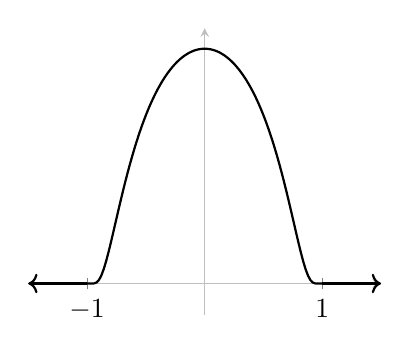
\begin{tikzpicture}
			\begin{axis}[
			xmin=-1.5,xmax=1.5,
			ymin=-0.05,ymax=0.4,
			ytick={0},
			xtick={-1,1},
			xticklabels={$-1$,1},
			yticklabels={},
			axis lines=middle,
			axis line style=lightgray,
			width=0.5\textwidth
			]
			
			
			\addplot[black,style=thick] expression[domain=-0.999:0.999,samples=100]{exp(-1/(1-x^2))}; 
			
			\addplot[black,style=thick,<-] expression[domain=-1.5:-1,samples=2]{0};
			
			\addplot[black,style=thick,->] expression[domain=1:1.5,samples=2]{0};
			\end{axis}
			\end{tikzpicture}
		\end{center}
		\caption{The graph of the function $\psi$ from \cref{canonical-bump}.}  \label{canonical-bump-graph}
	\end{figure}
\end{example}

\begin{exercise}
	For any $a < b$ in $\R$, construct a bump function $f : \R \to \R$ whose support is $[a,b]$. 
\end{exercise}

\begin{exercise}
	Let $F$ be a closed subset of $\R$. Construct a smooth function $f : \R \to \R$ which is zero on $F$ and nonzero outside of $F$. \begin{hint} Recall that the complement of $F$ is a countable disjoint union of open intervals (cf. \cite[theorem 6.17]{protter-morrey}). \end{hint}
\end{exercise}

\subsubsection*{Bridge functions}

Next up, we'll discuss an example of a ``bridge'' function.\index{bridge function@``bridge'' function} It will be constant on $(-\infty, -1]$, and also constant on $[1, \infty)$, but the values on these two intervals is different; and on $(-1,1)$, the function ``smoothly bridges the gap'' between the two values. 

In discussing this example, we will invoke the fundamental theorem of calculus,\index{fundamental theorem of calculus} even though we have not proved it (or even defined integrals, for that matter). If you're unhappy with using things you haven't proved, you can find rigorous discussions of integration in many places (eg, \cite[chapter 5]{protter-morrey}, \cite[chapter 6]{rudin}, etc). Alternatively, you might also be interested in \cite[chapter 3, example 12]{counterexamples}, which gives an example of a ``bridging function'' that involves no integrals (but does involve a double exponential). 

\begin{example} \label{bridge-function}
	Let $\psi$ be the bump function from \cref{canonical-bump}, and then consider 
	\[ \eta(x) = \int_{-1}^x \psi(t)\, dt. \]
	Then 
	\[ \eta'(x) = \frac{d}{dx} \int_{-1}^x \psi(t)\, dt = \psi(x) \]
	by the fundamental theorem of calculus. Thus $\eta$ is smooth, since $\eta' = \psi$ is smooth. Note moreover that $\eta$ is increasing, since $\eta' = \psi \geq 0$. Finally, it is clear from the geometric interpretation of integrals as ``area under the curve'' that $\eta$ is constantly equal to 0 for all $x \leq -1$ and that it is constantly equal to $\eta(1)$ for all $x \geq 1$. 
\end{example}

\begin{exercise} \label{constant-compact-zero-outside-neighborhood}
	For $a < b$ in $\R$, let $I = [a, b]$ and let $U$ be an open subset containing $I$. Prove that there exists a bump function $f : \R \to \R$ such that $f(x) = 1$ for all $x \in K$ and $f(x) = 0$ for all $x \notin U$. \begin{hint} 
	The characteristic function \[ \chi_I(x) = \begin{cases} 1 & \text{if } x \in I \\ 0 & \text{if } x \notin I \end{cases} \]
	is close to having all of the properties we want, but it's not smooth; it's clearly not even continuous. ``Bridge'' the discontinuities.\index{bridge function@``bridge'' function} \end{hint}
\end{exercise}

%TODO: Newton's method
	
	\chapter{Multivariable derivatives} \label{multi}

In this chapter, we will study derivatives of functions $S \to \R^n$ where $S$ is a subset of $\R^m$ and $m$ and $n$ are arbitrary positive integers. As it turns out, the most important case is when $n = 1$. In other words, the ``multi'' in the name of this chapter (as opposed to the ``single'' in the name of the previous chapter) is really referring to the fact that we might have multiple \emph{inputs} (ie, $m > 1$), rather than to the fact that we might have multiple outputs (ie, $n > 1$). The single variable case is actually quite important for the multivariable case; we'll often use results from \cref{single} to prove their multivariable counterparts. 

We'll begin by analyzing a particular example to build up some geometric intuition in \cref{multi-introductory-example}, before proceeding with the abstract discussion of multivariable derivatives. 

\section{Introductory example} \label{multi-introductory-example}

Recall that we started off our discussion of single variable derivatives starting with a very geometric idea of tangent lines to graphs. For large values of $m$ (and $n$), graphs become hard to visualize and it is not so clear what ``tangent'' should mean. But there is at least one multivariable situation where, by exerting some strain on the three-dimensional visualization sectors of our brain, we can geometrically formalize what ``tangent'' might mean. This is the $m = 2, n = 1$ situation. The graph of such a function is a surface in $\R^3$, and its ``tangent'' at a point should be a plane.  

By analyzing a specific function $f : \R^2 \to \R$,  we can get some valuable insights into multivariable derivatives; the analysis will presage many of the concepts we will discuss later in the chapter. Any function would do, but let's focus on the function $f : \R^2 \to \R$ defined by
\[ f(x, y) = x^2 + y^2 \]
for our analysis.  

\subsection*{Describing the graph of \texorpdfstring{$f$}{f}}

First off, let's try to get a solid understanding of the graph of $f$. The graph $\Gamma$ is a subset of $\R^2 \times \R = \R^3$ defined by
\[ \Gamma = \{ (x, y, z) : z = f(x, y) \} = \{ (x, y, z) : z = x^2  + y^2 \}. \]
It's a little hard to visualize in three dimensions immediately, so we will start by looking at two-dimensional slices of $\Gamma$, until we've seen enough slices that we have a sense of the three-dimensional geometry. 

If we consider the ``vertical'' slice obtained by setting $x = 0$, we find a parabola $z = y^2$. Similarly, if we consider the slice obtained by setting $x = 1$, we obtain the parabola $z = 1 + y^2$. Fixing $x = 5$, we obtain the parabola $z = 25 + y^2$. In fact, we can see that no matter what value of $x$ we fix, the resulting slice is always a parabola, just translated up from the origin by differing amounts; see \cref{multi-introductory-example-slices}. 

\begin{figure}[ht]
	\begin{center}
		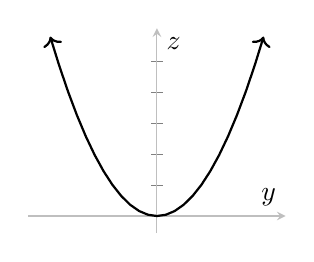
\begin{tikzpicture}
		\begin{axis}[
		xmin=-4.1,xmax=4.1,
		ymin=-1.1,ymax=12.1,
		xtick={0},
		ytick={2,4,6,8,10},
		yticklabels={},
		axis lines=middle,
		axis line style=lightgray,
		width=0.4\textwidth,
		xlabel={$y$},
		ylabel={$z$},
		]
		\addplot[black,style=thick,<->] expression[domain=-3.4:3.4,samples=25]{x^2}; 
		
		\end{axis}
		\end{tikzpicture}
		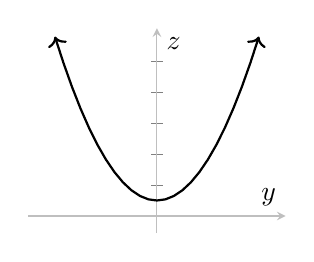
\begin{tikzpicture}
		\begin{axis}[
		xmin=-4.1,xmax=4.1,
		ymin=-1.1,ymax=12.1,
		xtick={0},
		ytick={2,4,6,8,10},
		yticklabels={},
		axis lines=middle,
		axis line style=lightgray,
		width=0.4\textwidth,
		xlabel={$y$},
		ylabel={$z$},
		]
		\addplot[black,style=thick,<->] expression[domain=-3.25:3.25,samples=25]{x^2+1}; 
		
		\end{axis}
		\end{tikzpicture}
		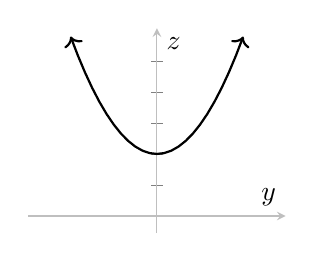
\begin{tikzpicture}
		\begin{axis}[
		xmin=-4.1,xmax=4.1,
		ymin=-1.1,ymax=12.1,
		xtick={0},
		ytick={2,4,6,8,10},
		yticklabels={},
		axis lines=middle,
		axis line style=lightgray,
		width=0.4\textwidth,
		xlabel={$y$},
		ylabel={$z$},
		]
		\addplot[black,style=thick,<->] expression[domain=-2.75:2.75,samples=25]{x^2+4}; 
		
		\end{axis}
		\end{tikzpicture}
	\end{center}
	\caption{Here are three vertical slices of the graph of the function $f(x,y) = x^2 + y^2$. From left to right, they are the $x = 0, x = 1$, and $x = 2$ slices, respectively.} \label{multi-introductory-example-slices}
\end{figure}

Slicing ``vertically in the other direction'' gives similar results. If we fix $y = 0$, we end up with the parabola $z = x^2$, and if we fix $y = 2$, we end up with the parabola $z = x^2 + 4$. 

It's also worth considering the ``level sets,'' ie, the ``horizontal'' slices of $\Gamma$ obtained by fixing various values of $z$. When $z = 0$, there is just the single point $x = y = 0$, ie, the origin. Fixing $z = 1$, the slice is given by $1 = x^2 +  y^2$, which is a circle of radius 1. Fixing $z = 17$, the slice is $17 = x^2 + y^2$, which is circle of radius $\sqrt{17}$. In fact, all of the level sets are circles, and these circles form a sort of ``topographic map'' style picture of the graph of $f$. See \cref{multi-introductory-example-level-sets}. 

\begin{figure}[ht]
	\begin{center}
		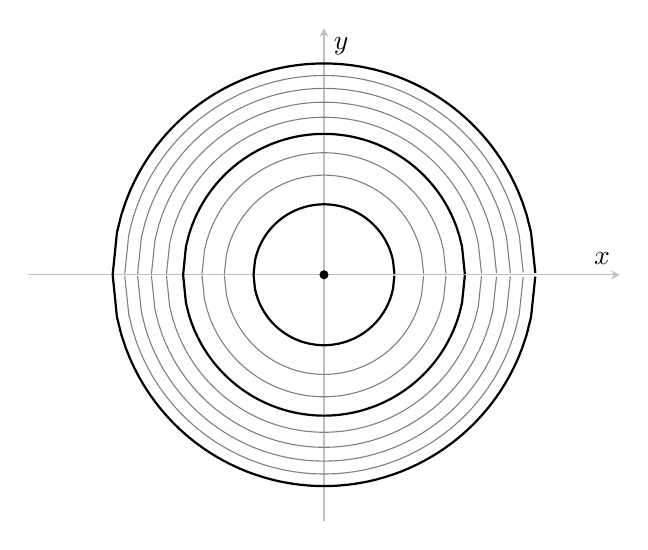
\begin{tikzpicture}
		\begin{axis}[
		xmin=-3.5,xmax=3.5,
		ymin=-3.5,ymax=3.5,
		xtick={0},
		ytick={0},
		xticklabels={},
		yticklabels={},
		axis lines=middle,
		axis line style=lightgray,
		width=0.75\textwidth,
		axis equal,
		xlabel={$x$},
		ylabel={$y$},
		]
		\node[color=black,draw=black,circle,fill,inner sep=1pt] at (axis cs:0,0) {};
		
		\addplot[black,style=thick,-] expression[domain=-1:1,samples=100]{sqrt(1-x^2)};
		\addplot[black,style=thick,-] expression[domain=-1:1,samples=100]{-sqrt(1-x^2)}; 
		
		\addplot[gray,-] expression[domain=-sqrt(2):sqrt(2),samples=100]{sqrt(2-x^2)};
		\addplot[gray,-] expression[domain=-sqrt(2):sqrt(2),samples=100]{-sqrt(2-x^2)}; 
		
		\addplot[gray,-] expression[domain=-sqrt(3):sqrt(3),samples=100]{sqrt(3-x^2)};
		\addplot[gray,-] expression[domain=-sqrt(3):sqrt(3),samples=100]{-sqrt(3-x^2)}; 
		
		\addplot[black,style=thick,-] expression[domain=-2:2,samples=100]{sqrt(4-x^2)};
		\addplot[black,style=thick,-] expression[domain=-2:2,samples=100]{-sqrt(4-x^2)}; 
		
		\addplot[gray,-] expression[domain=-sqrt(5):sqrt(5),samples=100]{sqrt(5-x^2)};
		\addplot[gray,-] expression[domain=-sqrt(5):sqrt(5),samples=100]{-sqrt(5-x^2)}; 
		
		\addplot[gray,-] expression[domain=-sqrt(6):sqrt(6),samples=100]{sqrt(6-x^2)};
		\addplot[gray,-] expression[domain=-sqrt(6):sqrt(6),samples=100]{-sqrt(6-x^2)}; 
		
		\addplot[gray,-] expression[domain=-sqrt(7):sqrt(7),samples=100]{sqrt(7-x^2)};
		\addplot[gray,-] expression[domain=-sqrt(7):sqrt(7),samples=100]{-sqrt(7-x^2)}; 
		
		\addplot[gray,-] expression[domain=-sqrt(8):sqrt(8),samples=100]{sqrt(8-x^2)};
		\addplot[gray,-] expression[domain=-sqrt(8):sqrt(8),samples=100]{-sqrt(8-x^2)}; 
		
		\addplot[black,style=thick,-] expression[domain=-3:3,samples=100]{sqrt(9-x^2)};
		\addplot[black,style=thick,-] expression[domain=-3:3,samples=100]{-sqrt(9-x^2)}; 
		 
		\end{axis}
		\end{tikzpicture}
	\end{center}
	\caption{Here is a ``topographic map'' style picture of the function $f(x,y) = x^2 + y^2$. Each circle is a level set of $f$. The innermost circle is the set of points such that $f(x,y) = 1$ (this is a circle of radius 1). The next circle from the inside (drawn in gray) is the set of points such that $f(x,y) = 2$ (this is a circle of radius $\sqrt{2}$). In general, the $k$th circle from the inside is the set of points such that $f(x,y) = k$. It is a circle of radius $\sqrt{k}$, and the circles where $\sqrt{k}$ is an integer are drawn in black rather than gray. The fact that the circles get ``closer together'' as $k$ increases is an indication that the function grows more and more rapidly as we get further from the origin. } \label{multi-introductory-example-level-sets}
\end{figure}


Stitching all of these two-dimensional slices together in our minds, we can see that the graph of $f$ is a ``big parabolic bowl'' inside $\R^3$. See \cref{multi-introductory-example-graph}. 

\begin{figure}[ht]
	\begin{center}
		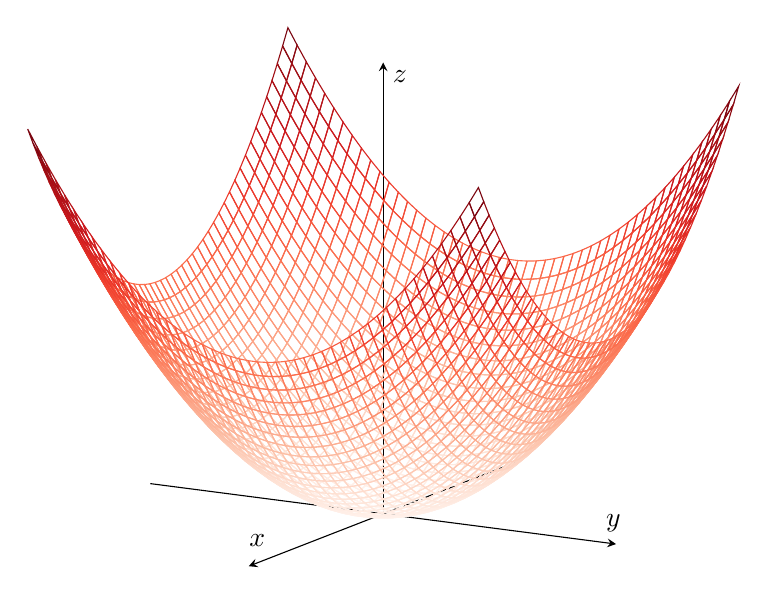
\begin{tikzpicture}
		\begin{axis}[
		view={120}{15},
		axis lines=middle,
		xlabel={$x$},
		xtick={0},
		xmin=-3.1,xmax=3.1,
		ylabel={$y$},
		ytick={0},
		ymin=-3.1,ymax=3.1,
		zlabel={$z$},
		ztick={0},
		zmin=0,zmax=20,
		width=0.9\textwidth,
		]
		\addplot3[mesh,samples=50,domain=-3:3,colormap/Reds]{x^2+y^2}; 
		\end{axis}
		\end{tikzpicture}
	\end{center}
	\caption{The graph of the function  $f(x,y) = x^2 + y^2$. ``Vertical'' slices (ie, slices along planes that are parallel to either the $xz$-plane or the $yz$-plane) are parabolas. ``Horizontal slices'' (ie, slices along planes parallel to the $xy$-plane) are circles.} \label{multi-introductory-example-graph}
\end{figure}

\subsection*{Tangent plane at \texorpdfstring{$a = (2,1)$}{a = (2,1)}}

Now that we understand what the graph of $f$ looks like, let's try to figure out what the ``tangent plane'' $T$ at a point $a = (2,1)$ will look like. Of course, it's a plane inside $\R^3$ that passes through the point $(2, 1, f(2,1)) = (2, 1, 5)$. To specify which plane it actually is, we start by describing some lines that lie on this plane. 

Consider the $y = 1$ slice of $\Gamma$, which is a vertical slice containing the point $a$. We know that the graph of $\Gamma$ along this slice is the parabola $z = x^2 + 1$. So, slicing the tangent plane $T$ along $y = 1$ should yield the tangent line to this function of one variable, which we know how to compute from \cref{single}. The slope of this tangent line is
\[ \left.\frac{d }{d x} f(x, 1) \right|_{x = 2} = 4. \]
This quantity is called a \emph{partial derivative of $f$ at $a$}, and will be denoted $(\partial f/\partial x)(a)$.  Thus the tangent line is the line parametrized by
\[ h \mapsto \begin{bmatrix} 2 \\ 1 \\ 5 \end{bmatrix} + h \begin{bmatrix} 1 \\ 0 \\ 4 \end{bmatrix}. \]
The vector $(1,0,4)$ records the fact that the tangent line moves up 4 units in the $z$-direction for every 1 unit that it moves in $x$-direction. 

Similarly, we can consider the $x = 2$ slice, which is another vertical slice containing $a$. We know that the graph $\Gamma$ along this slice is the parabola $z = 4 + y^2$.The slope of the corresponding tangent line is
\[ \frac{\partial f}{\partial y}(a) = \left.\frac{d f(2, y)}{dy}\right|_{y = 1} = 2. \]
Thus this tangent line is the line parametrized by
\[ k \mapsto \begin{bmatrix} 2 \\ 1 \\ 5 \end{bmatrix} + k \begin{bmatrix} 0 \\ 1 \\ 2 \end{bmatrix}. \]
Again, the vector $(1,0,2)$ records the fact that the tangent line moves up 4 units in the $z$-direction for every 1 unit that it moves in $y$-direction. See \cref{multi-introductory-example-graph-tangent-lines}.

\begin{figure}[ht]
	\begin{center}
		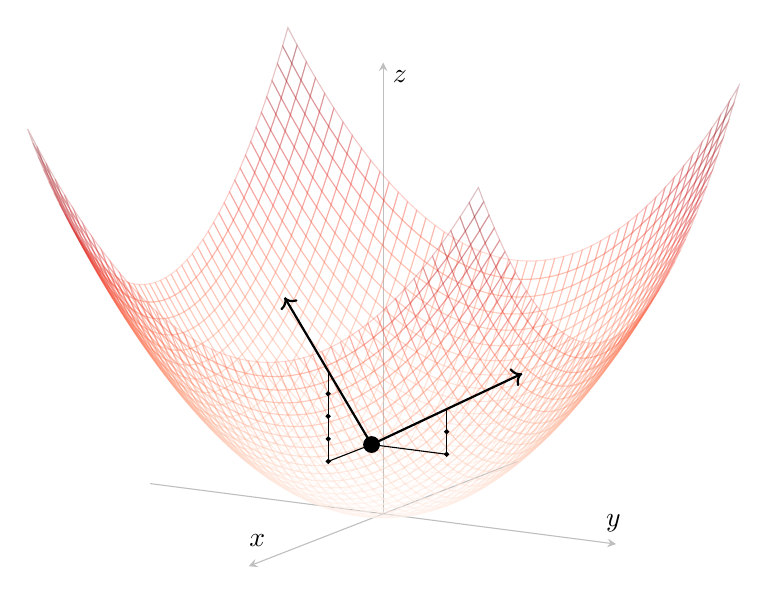
\begin{tikzpicture}
		\begin{axis}[
		view={120}{15},
		axis lines=middle,
		xlabel={$x$},
		xtick={0},
		xmin=-3.1,xmax=3.1,
		ylabel={$y$},
		ytick={0},
		ymin=-3.1,ymax=3.1,
		zlabel={$z$},
		ztick={0},
		zmin=0,zmax=20,
		width=0.9\textwidth,
		axis line style=lightgray,
		]
		\addplot3[mesh,samples=50,domain=-3:3,colormap/Reds,opacity=0.25]{x^2+y^2}; 
		\node[color=black,draw=black,circle,fill,inner sep=2pt] at (axis cs:2,1,5) {};
		
		\addplot3[variable=t,domain=0:2,color=black,thick,->] (2+t,1,5+4*t);
		\addplot3[variable=t,domain=0:1,color=black] (2+t,1,5);
		\addplot3[variable=t,domain=0:1,color=black] (3,1,5+4*t);
		\node[color=black,draw=black,circle,fill,inner sep=0.5pt] at (axis cs:3,1,5) {};
		\node[color=black,draw=black,circle,fill,inner sep=0.5pt] at (axis cs:3,1,6) {};
		\node[color=black,draw=black,circle,fill,inner sep=0.5pt] at (axis cs:3,1,7) {};
		\node[color=black,draw=black,circle,fill,inner sep=0.5pt] at (axis cs:3,1,8) {};
		
		\addplot3[variable=t,domain=0:2,color=black,thick,->] (2,1+t,5+2*t);
		\addplot3[variable=t,domain=0:1,color=black] (2,1+t,5);
		\addplot3[variable=t,domain=0:1,color=black] (2,2,5+2*t);
		\node[color=black,draw=black,circle,fill,inner sep=0.5pt] at (axis cs:2,2,5) {};
		\node[color=black,draw=black,circle,fill,inner sep=0.5pt] at (axis cs:2,2,6) {};
		\end{axis}
		\end{tikzpicture}
	\end{center}
	\caption{The graph of the function  $f(x,y) = x^2 + y^2$, together with the point $(a, f(a)) = (2,1,5)$ and two of its tangent lines: one parallel to the $xz$-plane, and the other parallel to the $yz$-plane.} \label{multi-introductory-example-graph-tangent-lines}
\end{figure}

These two tangent lines uniquely determine the entire tangent plane $T$ (ie, $T$ is the plane containing these two lines). One description that falls out immediately from the parametrizations of the tangent lines we found above is that $T$ is the plane parametrized by
\[ \begin{bmatrix} h \\ k \end{bmatrix} \mapsto \begin{bmatrix} 2 \\ 1 \\ 5 \end{bmatrix} + h \begin{bmatrix} 1 \\ 0 \\ 4 \end{bmatrix} + k \begin{bmatrix} 0 \\ 1 \\ 2 \end{bmatrix} = \begin{bmatrix} 2 \\ 1 \\ 5 \end{bmatrix} + \begin{bmatrix} h \\ k \\ 4h + 2k \end{bmatrix}. \]
As we've seen, the important part of this expression is the bottom entry on the far right, the $4h + 2k$. The function $\R^2 \to \R$ given by $(h, k)  \mapsto 4h + 2k$ is what we will call the \emph{differential} or the \emph{total derivative} of $f$, and denote by $df_a$. Notice that $df_a$ is a linear map $\R^2 \to \R$. Moreover, its graph is a plane passing through the origin that is parallel to $T$. In other words, if we take the graph of $df_a$ and translate it over to the point $(2,1,5)$, we obtain exactly the tangent plane $T$. Speaking more loosely, $df_a$ records all of the ``slopey information'' about the tangent plane $T$. 

Notice moreover that, if $e_1, e_2$ are the standard basis vectors of $\R^2$ (cf. \cref{euclidean}), then
\[ \begin{aligned} df_a(e_1) &= 4 = \frac{\partial f}{\partial x}(a) \\
df_a(e_2) &= 2 = \frac{\partial f}{\partial y}(a) \end{aligned} \]
so the standard matrix representation $[df_a]$ (cf. \cref{matrix-representation-standard}) of the linear map $df_a$ is \begin{equation} \label{jacobian-matrix-example} [df_a] = \begin{bmatrix} 4 & 2 \end{bmatrix} = \begin{bmatrix} \dfrac{\partial f}{\partial x}(a) & \dfrac{\partial f}{\partial y}(a) \end{bmatrix}. \end{equation}

\subsection*{\texorpdfstring{$df_a$}{dfa} as an approximation}

Consider the function $r : \R^2 \to \R$ defined by
\[ (h,k) \mapsto f(a+(h,k))-f(a)-df_a(h,k).  \]
This is the multivariable analog of the single variable remainder function from \cref{remainder-linear}. Then
\[ r(h,k) = (2+h)^2 + (1+k)^2 - 5 - 4h - 2k = h^2 + k^2. \]
Notice that $r$ gets small rapidly as $(h,k) \to 0$. More precisely, the claim is that
\[ \lim_{(h,k) \to 0} \frac{|r(h,k)|}{|(h,k)|} = 0, \]
ie, that $|r(h,k)| = o(|(h,k)|)$ as $(h,k) \to 0$. 

In fact, for the claim, it doesn't matter whether $|-|$ denotes the euclidean norm or the max norm (cf. \cref{euclidean}). If it's the euclidean norm, we have
\[ \lim_{(h,k) \to 0} \frac{|r(h,k)|}{|(h,k)|_2} = \lim_{(h,k) \to 0} = \frac{h^2 + k^2}{\sqrt{h^2 + k^2}} = \lim_{(h,k) \to 0} \sqrt{h^2 + k^2} = 0. \]
If instead it's the max norm, observe that
\[ \frac{|r(h,k)|}{|(h,k)|_\infty} = \frac{h^2 + k^2}{|(h,k)|_\infty} \leq \frac{2(|(h,k)|_\infty)^2}{|(h,k)|_\infty} = 2|(h,k)|_\infty \]
so taking the limit as $(h,k) \to 0$ and applying the squeeze theorem yields the same result. 

Since $r$ gets small rapidly, we can say that the function $(h,k) \mapsto f(a) + df_a(h,k)$ is a good approximation of the function $(h,k) \mapsto f(a+(h,k))$ for small vectors $(h,k)$. Said differently, letting $x = a + (h,k)$, the function $x \mapsto f(a) + df_a(x-a)$ is a good approximation of $f$ near $a$. 

\subsection*{Overview}

In what follows, we will turn the above example on its head and \emph{define} the differential $df_a$ to be a linear function which yields a good approximation of $f$ near a point $a$, and then we will prove in \cref{jacobian-matrix} that partial derivatives (ie, derivatives along various ``slices'') can be used to compute the standard matrix representation of the the differential. This might seem a bit ``backwards'' given our analysis of the example above, but there is a good reason for doing this; it turns out that there are some bizarre functions where partial derivatives make sense, but tangent planes do not.

Much of the discussion below will involve arbitrary $m$ and $n$, which is impossible to visualize. However, the $m = 2, n = 1$ situation already captures most of the complexity that arises in the multivariable setting. If you run into something that you looks overly abstract because of the general $m$ and $n$, try to understand it when $m = 2, n = 1$. 

We'll be using a lot of linear algebra in this chapter. The notation $|-|$ will denote either the euclidean or the max norm on $\R^n$, and you can choose to interpret it to be whichever of the two norms you like better (in the calculation we did above, the euclidean norm was a little easier; but, in general, I find the max norm to be far more convenient). When it makes a difference which of the two norms on $\R^n$ we have in mind, we'll specify this explicitly.  We'll also need some facts about the operator norm as we go along; I encourage you to at least skim through \cref{operator-norm-basic} before proceeding. 

\section{Definition of the derivative}

Throughout, $S$ will denote a subset of $\R^m$. 

\begin{definition}[Differentiability at a point] \index{differentiable!differentiable at a point}
	A function $f : S \to \R^n$ is \emph{differentiable at} an interior point $a \in S$ if there exists a linear map $\ell : \R^m \to \R^n$ such that
	\[ |f(a+h)-f(a)-\ell(h)| = o(|h|) \text{ as } h \to 0. \]
\end{definition}

It turns out that there exists at most one linear map that has the above property. 

\begin{lemma} \label{differential-unique}
	Suppose $f : S \to \R^m$ is differentiable at an interior point $a \in S$. If $\ell$ and $\ell'$ are both linear maps $\R^m \to \R^n$ such that
	\[ |f(a+h) - f(a) - \ell(h)| = o(|h|) \text { and } |f(a+h) - f(a) - \ell'(h)| = o(|h|) \text{ as } h \to 0, \]
	then $\ell = \ell'$. 
\end{lemma}

\begin{proof}
	Let $\phi = \ell' - \ell$. Then $\phi$ is also a linear map $\R^m \to \R^n$. Moreover, observe that
	\[ \begin{aligned} |\phi(h)| &= |\ell'(h) - \ell(h)| \\
	&= |(f(a+h)-f(a)-\ell(h))-(f(a+h)-f(a)-\ell'(h)| \\
	&\leq |f(a+h)-f(a)-\ell(h)| + |f(a+h)-f(a)-\ell'(h)|. \end{aligned} \]
	Since both $|f(a+h)-f(a)-\ell(h)|$ and $|f(a+h)-f(a)-\ell'(h)|$ are $o(|h|)$, \cref{less-than-small-is-small,little-o-vector-space} imply that $|\phi(h)| = o(|h|)$ also. Then \cref{linear-and-small} implies that $\phi = 0$. 
\end{proof}

\begin{exercise}
	Look at the exercises from \cref{prelims} that are invoked in the proof above (namely, \cref{less-than-small-is-small,little-o-vector-space,operator-norm-is-norm}) and do any of them that you haven't already done.
\end{exercise}

\Cref{differential-unique} tells us that the following definition makes sense.  

\begin{definition} 
	Suppose $f : S \to \R^n$ is differentiable at an interior point $a \in S$. Then the \emph{differential} or the \emph{total derivative of $f$ at $a$}, denoted $df_a$, is the unique linear map $\R^m \to \R^n$ satisfying
	\[ |f(a+h)-f(a)-df_a(h)| = o(|h|) \text{ as } h \to 0.  \]
\end{definition}

\begin{pedanticremark}
	Since we're using $|-|$ to refer indiscriminately to both the euclidean and max norms, it might be worth pointing out that the above definition is independent of which norm you have in mind. More precisely, for any linear function $\ell : \R^m \to \R^n$, it is true that $|f(a+h)-f(a)-\ell(h)|_2 = o(|h|_2)$ if and only if $|f(a+h)-f(a)-\ell(h)|_\infty = o(|h|_\infty)$. You might try proving this if you're interested; the key is \cref{max-euclidean}. The upshot is that the differential $df_a$ is a ``good'' approximation for $f(a+h)-f(a)$, independently of whether we're measuring distances using the euclidean norm or the max norm. 
\end{pedanticremark}

This definition is fairly difficult to use in practice. Only a handful examples can be computed directly from the definition. Here are some that I think are instructive.

\begin{example}[Derivative of multiplication] \label{derivative-of-multiplication}
	Let $\mu : \R^2 \to \R$ be the multiplication map $\mu(x, y) = xy$. Let us show that 
	\[ d\mu_{(a,b)}(h, k) = bh + ak \]
	for all $(a,b) \in \R^2$ and $(h,k) \in \R^2$. Let $\ell(h,k) = bh + ak$. Observe that 
	\[ \mu((a,b)+(h,k)) - \mu(a,b) - \ell(h,k) = (a+h)(b+k) - ab - bh - ak = hk, \]
	and it is true that $|hk| = o(|(h,k)|)$. Roughly, this is because $|hk|$ is ``quadratic,'' which should be smaller than the ``linearish'' $|(h,k)|$. 
	
	To check that $|hk| = o(|(h,k)|)$ formally, we have to choose either the euclidean or the max norm. Let's use the max norm; if you prefer the euclidean norm, I'll leave the euclidean version of the following for you to check yourself. We have $|hk| \leq |(h,k)|_\infty^2$ by definition, so 
	\[ \frac{|hk|}{|(h,k)|_\infty} \leq \frac{|(h,k)|_\infty^2}{|(h,k)|_\infty} = |(h,k)|_\infty. \]
	The right hand side tends to 0 as $(h,k) \to 0$, so the squeeze theorem guarantees that the left hand side tends to as well. In other words, we have shown that 
	\[ |\mu((a,b)+(h,k)) - \mu(a,b) - \ell(h,k)| = |hk| = o(|(h,k)|_\infty), \]
	proving that $\ell = d\mu_{(a,b)}$. 
\end{example}

\begin{exercise}[Derivative of division] \label{derivative-of-division}
	Let $U = \{(x,y) \in \R^2 : y \neq 0\}$ and let $\Delta : U \to \R$ be the division map $\Delta(x, y) = x/y$. Show that 
	\[ d\Delta_{(a,b)}(h, k) = \frac{bh - ak}{b^2}. \]
	for all $(a, b) \in U$ and $(h,k) \in \R^2$. 
\end{exercise}

\begin{exercise}[``Linear maps are their own derivatives''] \label{derivative-of-linear}
	Suppose $\ell : \R^m \to \R^n$ is a linear map. Prove that $d\ell_a = \ell$ for all $a \in \R^m$.  
\end{exercise}

\begin{exercise} \label{derivative-of-line}
	Suppose $v, w \in \R^n$ and $f : \R \to \R^n$ is given by $f(t) = v + tw$. Calculate $df_a$ for any $a \in \R$. What is $df_a(1)$?
\end{exercise}

We will develop a bit more theory in order to compute more effectively. Meanwhile, we can prove the following directly from the definition. 

\begin{exercise} \label{differentiable-implies-continuous}
	If $f : S \to \R^n$ is differentiable at an interior point $a \in S$, show that $f$ must be continuous at $a$. 
\end{exercise}

Of course, the converse to \cref{differentiable-implies-continuous} is false. We've seen single variable examples; here are some multivariable examples. 

\begin{example}
	Consider the euclidean norm function $f : \R^2 \to \R$, given by 
	\[ f(x,y) = \sqrt{x^2 + y^2}. \]
	See \cref{euclidean-norm-graph}. This is definitely continuous at the origin, but the ``point'' of the cone at the origin suggests that this function is not differentiable at 0. Let's check this directly from the definition. 
	
	\begin{figure}[ht]
		\begin{center}
			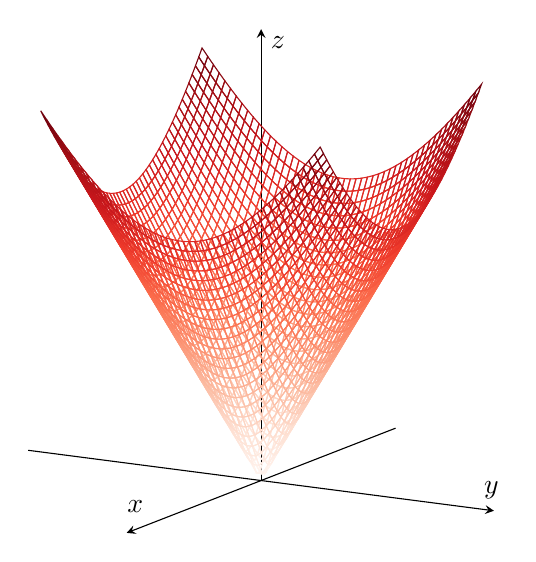
\begin{tikzpicture}
			\begin{axis}[
			view={120}{15},
			axis lines=middle,
			xlabel={$x$},
			xtick={0},
			xmin=-5,xmax=5,
			ylabel={$y$},
			ytick={0},
			ymin=-5,ymax=5,
			zlabel={$z$},
			ztick={0},
			zmin=0,zmax=5,
			width=0.9\textwidth,
			]
			\addplot3[mesh, colormap/Reds, samples=50, domain=-3:3]{sqrt(x^2 + y^2)};
			\end{axis}
			\end{tikzpicture}
		\end{center}
		\caption{The graph of the function  $f(x,y) = \sqrt{x^2 + y^2}$ is an infinite cone, extending upwards, with its point at the origin.} \label{euclidean-norm-graph}
	\end{figure}
	
	Suppose for a contradiction that $f$ were differentiable at the origin. Then there would exist a linear map $\ell(h,k) = ah + bk$ such that $|f(h,k) - f(0) - \ell(h,k)| = o(|(h,k)|)$. 
	Observe that
	\[ |f(h,k) - f(0) - \ell(h,k)| = |\sqrt{h^2 +  k^2} - ah - bk|. \]
	Intuitively, notice that $\sqrt{h^2 + k^2}$ is ``linearish,'' and $ah + bk$ is definitely linear; so the difference should also be ``linearish,'' but the only way a ``linearish'' function can be $o(|(h,k)|)$ is if it's zero. But $\sqrt{h^2 + k^2}$ is not actually linear, so there cannot not exist $a$ and $b$ such that $\sqrt{h^2 + k^2} = ah + bk$. The conclusion of this intuitive argument is that it should be impossible for $|\sqrt{h^2 + k^2} - ah - bk|$ to be $o(|(h,k)|)$, no matter what $a$ and $b$ are. 
	
	More formally, we want to find a contradiction to the assertion that
	\[ \lim_{(h,k) \to 0} \frac{|\sqrt{h^2 + k^2} - ah - bk|}{|(h,k)|} = 0. \]
	If we approach the origin along the line $k = 0$, this says that
	\[ 0 = \lim_{h \to 0} \frac{|\sqrt{h^2} - ah|}{|h|} = \lim_{h \to 0} \left| \frac{|h|}{h} - a \right| \quad\implies\quad \lim_{h \to 0} \frac{|h|}{h} = a.  \]
	But this is nonsense, since $|h|/h$ does not converge at all as $h \to 0$. It tends to 1 as $h \to 0^+$ and to $-1$ as $h \to 0^-$. 
\end{example}

\begin{exercise} \label{continuous-not-differentiable}
	Consider the function $f : \R^2 \to \R$ given by \[ f(x,y) = \sqrt{|xy|}. \]
	See \cref{sqrt-x-y-graph}. Show that $f$ is continuous at the origin, but that it is not differentiable at the origin. 
	\begin{hint}
		If $f$ were differentiable at the origin, then there would exist $a, b \in \R$ such that 
		\[ \lim_{(h,k) \to 0} \frac{|f(h,k) - ah -  bk|}{|(h,k)|} = 0. \]
		Think about what happens with this limit when you approach the origin along the line $k = 0$, along the line $h = 0$, and along the line $h = k$.
	\end{hint}
	\begin{figure}[ht]
		\begin{center}
			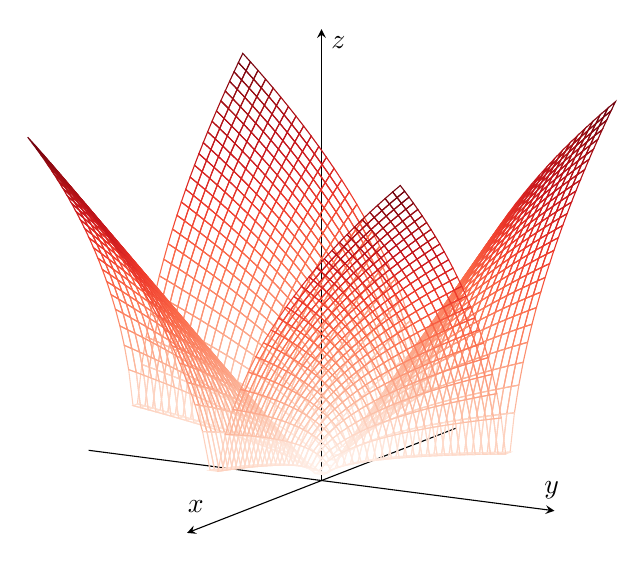
\begin{tikzpicture}
			\begin{axis}[
			view={120}{15},
			axis lines=middle,
			xlabel={$x$},
			xtick={0},
			xmin=-5,xmax=5,
			ylabel={$y$},
			ytick={0},
			ymin=-5,ymax=5,
			zlabel={$z$},
			ztick={0},
			zmin=0,zmax=5,
			width=0.9\textwidth,
			]
			\addplot3[mesh, colormap/Reds, samples=50, domain=-4:4]{sqrt(abs(x*y))};
			\end{axis}
			\end{tikzpicture}
		\end{center}
		\caption{The graph of the function  $f(x,y) = \sqrt{|xy|}$. The graph has four ``leaves,'' which look a bit like the ``leaves'' of the Sydney Opera House, or of the Lotus Temple in New Delhi.} \label{sqrt-x-y-graph}
	\end{figure}
\end{exercise}

\begin{exercise} \label{differentiable-at-a-point-but-not-in-any-neighborhood}
	Describe the set of all points $(a, b) \in \R^2$ where the function $f : \R^2 \to \R$ given by \[ f(x,y) = |xy| \] is not differentiable. 
\end{exercise}

\section{Computing derivatives}

\subsection{Sum and scalar multiples rule} 

\begin{exercise}[Sum rule] \label{sum-rule} \index{sum rule}
	Prove that, if $f, g : S \to \R^n$ are both differentiable at an interior point $a \in S$, then $f + g$ is also differentiable at $a$ and \[ d(f+g)_a = df_a + dg_a. \]
\end{exercise}

\begin{solution}{\cref{sum-rule}}
	Observe that 
	\[ |(f+g)(a+h)-(f+g)(a)-(df_a+dg_a)(h)| = |f(a+h) - f(a) - df_a(h) + g(a+h) - g(a) - dg_a(h)| \leq |f(a+h) - f(a) - df_a(h)| + |g(a+h) - g(a) - dg_a(h)|. \]
	Both $|f(a+h) - f(a) - df_a(h)|$ and $|g(a+h) - g(a) - dg_a(h)|$ are $o(|h|)$ by definition of the derivative, so it follows from \cref{little-o-vector-space,less-than-small-is-small} that $|(f+g)(a+h)-(f+g)(a)-(df_a+dg_a)(h)|$ is $o(|h|)$. Thus $df_a + dg_a = d(f+g)_a$. 
\end{solution}

\begin{exercise}[Scalar multiples rule] \label{scalar-multiples-rule} \index{scalar multiples rule}
	Prove that, if $c$ is a constant and $f : S \to \R^n$ is differentiable at an interior point $a \in S$, then $cf$ is also differentiable at $a$ and \[ d(cf)_a = c \cdot df_a. \]
\end{exercise}

\subsection{Chain rule}

The proof of the following is essentially the same as the second proof of the single variable chain rule given in \cref{chain-rule-single-section}. Since this proof is basically a repeat, some details are omitted; you are asked to fill in the details in \cref{chain-rule-details} below. 

\begin{theorem}[Chain rule] \label{chain-rule} \index{chain rule}
	Suppose that $S$ and $T$ are subsets of $\R^m$ and $\R^n$, respectively, that $f : S \to \R^n$ is differentiable at an interior point $a$, that $f(S) \subseteq T$ and $f(a)$ is an interior point of $T$, and that $g : T \to \R^p$ is differentiable at $f(a)$. Then the composite $g \circ f : S \to \R^p$ is also differentiable at $a$, and 
	\[ d(g \circ f)_a = dg_{f(a)} \circ df_a. \]
\end{theorem}

\begin{proof}
	Define the ``error in approximation'' functions\index{error in approximation function@``error in approximation'' function}
	\[ \begin{aligned} 
	r(h) &= f(a+h)-f(a) - df_a(h) \\ 
	s(k) &= g(f(a)+k)-g(f(a))-dg_{f(a)}(k) 
	\end{aligned} \]
	and then observe that
	\begin{equation} \label{rewrite-error} g(f(a+h)) - g(f(a)) - dg_{f(a)}(df_a(h)) = dg_{f(a)}(r(h)) + s(df_a(h)+r(h)). \end{equation}
	This means that 
	\[ |g(f(a+h)) - g(f(a)) - dg_{f(a)}(df_a(h))| \leq |dg_{f(a)}(r(h))| + |s(df_a(h)+r(h))|. \]
	Since $dg_{f(a)}$ is linear and $|r(h)| = o(|h|)$, \cref{chain-rule-details} guarantees that $|dg_{f(a)}(r(h))| = o(|h|)$ also. Thus, by \cref{little-o-vector-space}, it is sufficient to prove that $|s(df_a(h) + r(h))| = o(|h|)$. To do this, define $\eta(k) = |s(k)|/|k|$ and then notice that 
	\[ \begin{aligned} \frac{|s(df_a(h)+r(h))|}{|h|} &= \eta(df_a(h)+r(h)) \cdot \frac{|df_a(h) + r(h)|}{|h|} \\
	&\leq \eta(df_a(h) + r(h)) \left( \|df_a\| + \frac{|r(h)|}{|h|} \right) \end{aligned} \]
	where we have used \cref{operator-norm-reformulation} for the inequality.
	We now take the limit as $h \to 0$. Using the facts that $\eta \circ (df_a + r)$ is continuous at 0 and that $|r(h)| = o(|h|)$, we obtain the result. 
\end{proof}

\begin{exercise} \label{chain-rule-details}
	\begin{enumerate}[(a)]
		\item Prove \cref{rewrite-error}. 
		
		\item Do \cref{operator-norm-reformulation} if you haven't already. 
		
		\item \label{linear-of-small-is-small} Suppose $r : \R^m \to \R^n$ is a function such that $|r(h)| = o(|h|)$ as $h \to 0$. If $\ell : \R^n \to \R^p$ is linear, prove that $|\ell(r(h))| = o(|h|)$ also.
		
		\begin{hint} Even though the operator norm\index{operator norm} does not appear anywhere in the statement of this exercise, you might find the concept useful (especially \cref{operator-norm-reformulation}). 
		\end{hint}
		
		\item Prove that $\eta \circ (df_a + r)$ is continuous at 0. 
	\end{enumerate}
\end{exercise}

\begin{comment}
\begin{proof}
Observe that
\[ \frac{|\ell(r(v))|}{|v|} \leq \frac{\|\ell\| \cdot |r(v)|}{|v|}. \]
Since $|r(v)| = o(|v|)$, we see that the right-hand side tends to 0 as $v \to 0$. The squeeze theorem thus guarantees that $|\ell(r(v))| = o(|v|)$ also. 
\end{proof}
\end{comment}

\subsection{Differentiability by components}

Recall that we asserted at the beginning of this chapter that the ``multi'' in the name of this chapter refers to the number of inputs (rather than the number of outputs). This section is where we show that understanding the $n = 1$ case is ``enough'' to understand general $n$.

\begin{definition}[Component functions] \index{component function}
	For any function $f : S \to \R^n$, we define the $j$th \emph{component function} $f_j : S \to \R$ to be the composite $\pi_j \circ f$, where $\pi_j$ is the $j$th projection map (cf. \cref{euclidean}).\index{projection map}
\end{definition}

\begin{proposition} \label{differentiable-by-components}
	A function $f : S \to \R^n$ is differentiable at an interior point $a \in S$ if and only if the component function $f_j : S \to \R$ is differentiable at $a$ for all $j = 1, \dotsc n$. Moreover,
	\begin{equation} \label{derivative-of-components} df_a(h) = \begin{bmatrix} df_{1,a}(h) \\ \vdots \\ df_{n,a}(h) \end{bmatrix}. \end{equation}
\end{proposition}

\begin{proof}
	If $f$ is differentiable at $a$, then the composite $f_j = \pi_j \circ f$ is also differentiable at $a$ by the chain rule \ref{chain-rule}. Moreover, since $\pi_j$ is linear, we know that $d\pi_{j,f(a)} = \pi_j$ by \cref{derivative-of-linear}. Thus, by the chain rule, 
	\[ df_{j,a}(h) = (d\pi_{j,f(a)} \circ df_a)(h) = \pi_j(df_a(h)) \]
	for all $j$, which is precisely \cref{derivative-of-components}. 
	For the converse, we turn \cref{derivative-of-components} on its head. Suppose $f_j$ is differentiable at $a$ for all $j$, and let $\ell : \R^m \to \R^n$ be the linear map 
	\[ \ell(h) = \begin{bmatrix} df_{1,a}(h) \\ \vdots \\ df_{n,a}(h) \end{bmatrix}.  \]
	We now want to show that $|f(a+h)-f(a)-\ell(h)| = o(|h|)$ as $h \to 0$. Observe that the component functions of $h \mapsto f(a+h)-f(a)-\ell(h)$ are given by
	\[ v \mapsto \pi_j \left( f(a+h)-f(a)-\ell(h) \right) = f_j(a+h)-f_j(a)-df_{j,a}(h) \]
	since $\pi_j$ is linear, 
	and we know that $|f_j(a+h)-f_j(a)-df_{j,a}(h)| = o(|h|)$. By \cref{components-are-small-implies-small} below applied with the function $r(h) = f(a+h)-f(a)-\ell(h)$, we conclude that $|f(a+h)-f(a)-\ell(h)| = o(|h|)$. 
\end{proof}

\begin{exercise} \label{components-are-small-implies-small}
	Show that if $S$ is a neighborhood of 0 in $\R^m$ and $r :  S  \to \R^n$ is a function such that $|r_j(h)| = o(|h|)$ as $h \to 0$ for all $j = 1, \dotsc, n$, then $|r(h)| = o(|h|)$ also.
	\begin{hint}
		This is easy if you're using the max norm. If you're using the euclidean norm, you may find it useful to do \cref{max-euclidean} first. 
	\end{hint}
\end{exercise}

\begin{exercise}
	Suppose $S$ is a subset of $\R$ and $f : S \to \R^n$ is differentiable at an interior point $a$. Show that the standard matrix representation $[df_a]$ of the linear map $df_a : \R \to \R^nn$ is given by 
	\[ [df_a] = \begin{bmatrix} f_1'(a) \\ \vdots \\ f_n'(a) \end{bmatrix}, \]
	where $f_j'(a)$ is the derivative of the single variable function $f_j : S \to \R$ in the sense of \cref{single}. 
\end{exercise}

\subsection{Product and quotient rules}

We showed in the previous section that it's enough to understand the $n = 1$ case, ie, the case of real-valued (rather than $\R^n$-valued) functions. So in this section and the next, we'll focus our attention on real-valued functions. 

Note that we can combine real-valued functions in more ways than the ones we've already discussed; specifically, we can multiply and divide them. As in \cref{single}, we have product and quotient rules to deal with this. As it turns out, we can actually derive these using the multivariable chain rule \ref{chain-rule}!

\begin{proposition}[Product rule] \label{product-rule} \index{product rule}
	Suppose $f, g : S \to \R$ are both differentiable at an interior point $a \in S$. Then $fg$ is also differentiable at $a$ and
	\[ d(fg)_a = g(a)df_a + f(a) dg_a. \]
\end{proposition}

\begin{proof}
	Let $f \times g$ denote the function $S \to \R^2$ defined by
	\[ (f \times g)(x) = (f(x), g(x)). \]
	Observe that the first and second component functions of $f \times g$ are $f$ and $g$, respectively; thus it follows from \cref{differentiable-by-components} that 
	\[ d(f \times g)_a(h) = (df_a(h), dg_a(h)). \]
	Let $\mu : \R^2 \to \R$ denote the multiplication map $\mu(x,y) = xy$ that we considered in \cref{derivative-of-multiplication}. Then $fg = \mu \circ (f \times g)$, so by the chain rule \ref{chain-rule}, we have that 
	\[ \begin{aligned} d(fg)_a(h) &= d\mu_{(f(a),g(a))}(d(f \times g)_a(h)) \\
	&= d\mu_{f(a),g(a)}(df_a(h), dg_a(h)) \\
	&= g(a) df_a(h) + f(a)dg_a(h), \end{aligned} \]
	where we have used the calculation from \cref{derivative-of-multiplication} for the final step. 
\end{proof}

\begin{exercise} \label{reciprocal-rule}
	Suppose $f : S \to \R$ is differentiable at an interior point $a \in S$ and that $f(a) \neq 0$. Show that $1/f$ is also differentiable at $a$, and
	\[ d(1/f)_a = -\frac{df_a}{f(a)^2}.  \]
	\begin{hint}
		Consider the function $\iota : \R \setminus \{0\} \to \R$ given by $\iota(x) = 1/x$. This is a single variable function, so we know $d\iota_x$ from \cref{single}. Now note that $1/f = \iota \circ f$. 
	\end{hint}
\end{exercise}

\begin{exercise}[Quotient rule] \label{quotient-rule} \index{quotient rule}
	Suppose $f, g : S \to \R$ is differentiable at an interior point $a \in S$ and that $g(a) \neq 0$. Show that $f/g$ is also differentiable at $a$, and that
	\[ d(f/g)_a = \frac{g(a)df_a - f(a)dg_a}{g(a)^2}. \]
	\begin{hint}
		One approach is to combine \cref{reciprocal-rule} and the product rule \ref{product-rule}. An alternative approach is to mimic the proof of the product rule \ref{product-rule} (using the division function of \cref{derivative-of-division} in place of the multiplication function of  \cref{derivative-of-multiplication}). 
	\end{hint}
\end{exercise}

\subsection{Directional and partial derivatives}

We now formalize the ``slicing'' we did in \cref{multi-introductory-example}. 

\begin{definition}[Directional derivatives] \index{directional derivative} \index{partial derivative}
	Suppose $f : S \to \R$ is a function, $a \in S$ is an interior point, and $h \in \R^m$ is a vector. The \emph{directional derivative of $f$ at $a$ with respect to $h$}, denoted $\partial_h f(a)$, is defined to be the limit
	\[ \lim_{t \to 0} \frac{f(a+th) - f(a)}{t}. \]
	If $h = e_i$ is the $i$th standard basis vector (cf. \cref{euclidean}), then this is called the \emph{$i$th partial derivative of $f$ at $a$} and denoted $\partial_i f(a)$ (instead of $\partial_{e_i} f(a)$). If we're using $x_i$ to denote the $i$th component of the input of $f$, then $\partial_i f(a)$ is sometimes also denoted by one of the following. 
	\[ f_{x_i}(a) \quad \left. \frac{\partial f}{\partial x_i}\right|_{x = a} \quad \left.\frac{\partial}{\partial x_i} f(x)\right|_{x = a} \quad \frac{\partial f}{\partial x_i}(a) \]
\end{definition}

You may remember from multivariable calculus that partial derivatives behave a great deal like single variable derivatives. The reason for this is the following important remark, which reinterprets a directional derivative as a single variable derivative. 

\begin{remark} \label{directional-to-single}
	For $a \in S$ an interior point and $h \in \R^m$, consider the function $\xi : \R \to \R^m$ given by $\xi(t) = a + th$. This is the ``line through $a$ in the direction of the vector $h$.'' Note that $0 = \xi^{-1}(a)$ is an interior point of $\xi^{-1}(S)$ since $a$ is a interior point of $S$. If $f : S \to \R$ is a function, then $f \circ \xi$ is a single variable function $\xi^{-1}(S) \to \R$, and we have
	\[ \partial_h f(a) = (f \circ \xi)'(0), \]
	just by writing out the definition of both sides. A bit more geometrically, $f \circ \xi$ can be thought of as the restriction of $f$ to the line passing through $a$ in the direction of $h$. This is a single variable function, and the derivative of this single variable function at 0 is the directional derivative of $f$ at $a$ with respect to $h$. 
\end{remark}

\begin{example} \label{computing-partials-example}
	Consider the function $f : \R^2 \to \R$ given by $f(x, y) = \sin(xy^2)$. Fix $(a, b) \in \R^2$ and define $\xi : \R \to \R^2$ by $\xi(t) = (a + t, b)$. In other words, $\xi$ is the line through $(a, b)$ in the direction of the vector $(1,0)$, as in \cref{directional-to-single}. Then
	\[ (f \circ \xi)(t) = f(a + t, b) = \sin((a+t)b^2).  \]
	Then
	\[ \begin{aligned} \frac{\partial f}{\partial x}(a, b) &= (f \circ \xi)'(0) \\
	&= \left.\frac{d}{dt} \left(\sin((a+t)b^2) \right) \right|_{t = 0} \\
	&= \left. b^2\cos((a+t)b^2)\right|_{t = 0} \\
	&= b^2\cos(ab^2). \end{aligned}  \]
\end{example}

\begin{exercise}
	With notation as in \cref{computing-partials-example}, compute $(\partial f/\partial y)(a, b)$. 
\end{exercise}

\begin{exercise} \label{basic-directional-derivative-properties}
	Suppose $f : S \to \R$ is a function and $a \in S$ is an interior point. Prove the following. 
	\begin{enumerate}[(a)]
		\item $\partial_0 f(a) = 0$.  
		\item If $\partial_h f(a)$ exists for some $h \in \R^m$, then $\partial_{\lambda h} f(a)$ also exists for all $\lambda \in \R$ and \[ \partial_{\lambda h} f(a) = \lambda \partial_h f(a). \] 
	\end{enumerate}
\end{exercise}

We can use \cref{directional-to-single} to prove some directional derivative analogs of results we proved in \cref{single}.

\begin{exercise}[Product rule for directional derivatives] \label{product-rule-directional} \index{product rule}
	Suppose $f, g : S \to \R$ are functions, $a \in S$ is an interior point, and $h \in \R^m$ is a vector such that $\partial_h f(a)$ and $\partial_h g(a)$ both exist. Prove that $\partial_h (fg)(a)$ also exists and that
	\[ \partial_h (fg)(a) = g(a)\partial_h(f)(a) + f(a) \partial_h g(a). \]
	\begin{hint} 
		Use \cref{directional-to-single} and the single variable product rule \ref{product-rule-single}.
	\end{hint}
\end{exercise}

\begin{exercise}[Quotient rule for directional derivatives] \label{quotient-rule-directional} \index{quotient rule}
	Suppose $f, g : S \to \R$ are functions, $a \in S$ is an interior point such that $g(a) \neq 0$ and $\partial_h f(a)$ and $\partial_h g(a)$ both exist for some $h \in \R^m$. Show that $\partial_h(f/g)(a)$ also exists and 
	\[ \partial_h(f/g)(a) = \frac{g(a)\partial_h f(a) - f(a)\partial_h g(a)}{g(a)^2}. \]
	\begin{hint} Use \cref{directional-to-single} and the single variable quotient rule \ref{quotient-rule-single}. \end{hint} 
\end{exercise}

\begin{exercise}[Interior extremum theorem for directional derivatives] \label{interior-extremum-directional} \index{extremum!interior extremum theorem}
	Suppose $f : S \to \R$ is a function and an interior point $a \in S$ is a local extremum of $f$. Show that, if $\partial_h f(a)$ exists for some $h \in \R^m$, then $\partial_h f(a) = 0$. 
	\begin{hint} Use \cref{directional-to-single} and the single variable interior extremum theorem \ref{interior-extremum}. \end{hint}
\end{exercise}

Just as the converse to the single variable interior extremum theorem \ref{interior-extremum} is false (cf. \cref{interior-extremum-converse-false}), so too is the converse to the interior extremum theorem for directional derivatives \ref{interior-extremum-directional}, except that there are now even more ways for the converse to fail. Here are some examples to illustrate this.  

\begin{example} \label{saddle}
	Consider the function $f : \R^2 \to \R$ given by \[ f(x, y) = x^2 - y^2. \]
	Let $\xi(t) = 0 + te_1 = (t, 0)$. Then $f \circ \xi$ has a minimum at 0, so $(f \circ \xi)'(0) = (\partial f)/(\partial x)(0) = 0$. Similarly, if $\xi(t) = 0 + te_2 = (0, t)$, then $f \circ \xi$ has a maximum at 0, so $(f \circ \xi)'(0) = (\partial f)/(\partial y)(0) = 0$ also. But clearly these two facts together mean that 0 cannot be a local extremum of $f$. See \cref{saddle-graph}. This kind of a point is sometimes called a ``saddle.''\index{saddle}
	\begin{figure}[ht]
		\begin{center}
			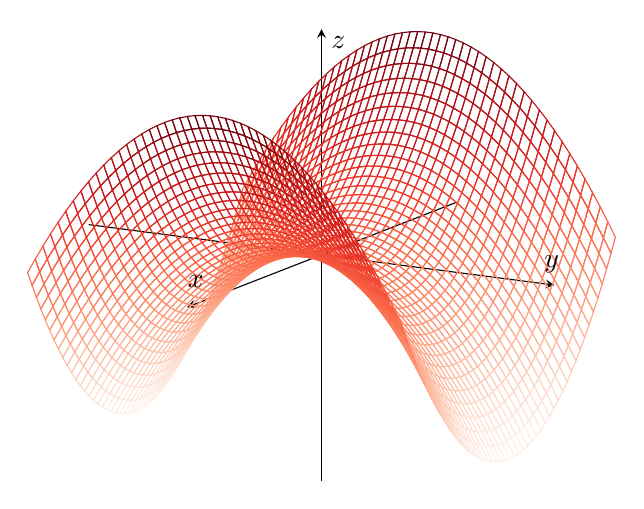
\begin{tikzpicture}
			\begin{axis}[
			view={120}{15},
			axis lines=middle,
			xlabel={$x$},
			xtick={0},
			xmin=-5,xmax=5,
			ylabel={$y$},
			ytick={0},
			ymin=-5,ymax=5,
			zlabel={$z$},
			ztick={0},
			zmin=-20,zmax=20,
			width=0.9\textwidth,
			]
			\addplot3[mesh,samples=50,domain=-4:4,
			colormap/Reds]{x^2-y^2};
			\end{axis}
			\end{tikzpicture}
		\end{center}
		\caption{The graph of the function  $f(x,y) = x^2 - y^2$. Vertical slices along planes parallel to the $xz$-plane are downwards facing parabolas, while those along planes parallel to the $yz$-plane are upwards facing parabolas.} \label{saddle-graph}
	\end{figure}
\end{example}

\begin{exercise} \label{all-directionals-vanish-but-not-extremum}
	Consider the function $f : \R^2 \to \R$ given by 
	\[ f(x, y) = (y- x^2)(y - 3x^2). \]
	See \cref{all-directionals-vanish-but-not-extremum-graph} for the graph of $f$. 
	\begin{figure}[ht]
		\begin{center}
			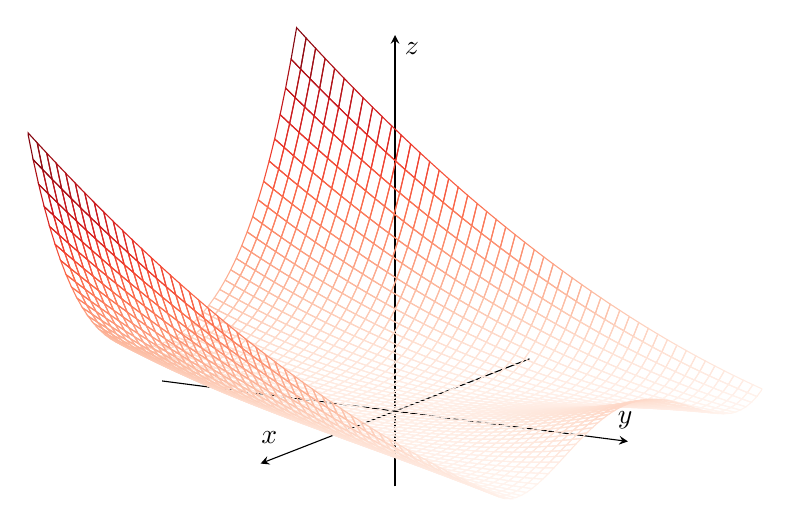
\begin{tikzpicture}
			\begin{axis}[
			view={120}{15},
			axis lines=middle,
			xlabel={$x$},
			xtick={0},
			xmin=-1,xmax=1,
			ylabel={$y$},
			ytick={0},
			ymin=-1,ymax=1,
			zlabel={$z$},
			ztick={0},
			zmin=-2,zmax=10,
			width=0.9\textwidth,
			]
			\addplot3[mesh,samples=50,domain=-1:1,
			colormap/Reds]{(y- x^2)*(y - 3*x^2)};
			\end{axis}
			\end{tikzpicture}
		\end{center}
		\caption{The graph of the function  $f(x,y) = (y- x^2)(y - 3x^2)$.} \label{all-directionals-vanish-but-not-extremum-graph}
	\end{figure}
	\begin{enumerate}[(a)]
		\item Show that the origin is \emph{not} a local extremum of $f$. \begin{hint} Consider the values of $f$ on points of the form $(0,b)$ and $(a, 2a^2)$ near the origin. You might consider identifying where these points are on the graph depicted in \cref{all-directionals-vanish-but-not-extremum-graph} to get a more visual sense of what's going on. \end{hint}
		\item Show that $f$ has a local minimum when restricted to an arbitrary line through the origin. Conclude that $\partial_h f(a) = 0$ for all $h \in \R^2$. 
	\end{enumerate}
\end{exercise}

\begin{exercise}
	Consider the function $f : \R^2 \to \R$ given by
	\[ f(x,y) = 2x^3 - 3x^2 + 2y^3 + 3y^2. \]
	Find all points $a \in \R^2$ such that $\partial_1 f(a) = \partial_2 f(a) = 0$. Of these points, which (if any) are local extremums? 
\end{exercise}

Now for the main result of this section, which relates the differential to directional derivatives. Note that we will generalize this result slightly in \cref{jacobian-matrix} below. 

\begin{proposition} \label{differentiable-implies-directionals}
	If $f : S \to \R$ is differentiable at an interior point $a \in S$ and $h \in \R^m$, then \[ df_a(h) = \partial_h f(a). \]
	Thus, the standard matrix representation $[df_a]$ of the total derivative $df_a : \R^m \to \R$ is a $1 \times m$ matrix whose $i$th entry is the $i$th partial derivative $\partial_i f(a)$. 
	\[ [df_a] = \begin{bmatrix} \partial_1 f(a) & \partial_2 f(a) & \dotsb & \partial_m f(a) \end{bmatrix} \]
\end{proposition}

\begin{proof}
	If $h = 0$, we know that $\partial_0 f(a) = 0$ by \cref{basic-directional-derivative-properties} and that $df_a(0) = 0$ since $df_a$ is linear, so we are done. Thus we can assume that $h$ is nonzero. Let $r$ be the ``error in approximation'' function
	\[ r(k) = f(a+k) - f(a) - df_a(k), \]
	so that $|r(k)| = o(|k|)$ as $k \to 0$. Letting $k = th$, we see that
	\[ r(th) = f(a+th) - f(a) - df_a(th) = f(a+th) - f(a) - t df_a(h) \]
	by linearity of $df_a$, so
	\[ \frac{r(th)}{t} = \frac{f(a+th) - f(a) - tdf_a(h)}{t} = \frac{f(a+th) - f(a)}{t} - df_a(h). \]
	Then 
	\[\lim_{t \to 0} \left| \frac{f(a+th) - f(a)}{t} - df_a(h) \right| 
	= \lim_{t \to 0} \frac{|r(th)|}{|t|} = \lim_{t \to 0} \frac{|r(th)|}{|th|} \cdot |h| = 0 \]
	where we used the fact that $|r(k)| = o(|k|)$ as $k \to 0$ for the last step. This tells us that $\partial_h f(a)$ exists and equals $df_a(h)$. In particular, applying this with $h = e_i$, we see that $df_a(e_i) = \partial_i f(a)$, which yields the standard matrix representation.  
\end{proof}

\begin{remark} \label{gradient}
	If $f : S \to \R$ is differentiable at an interior point $a \in S$, the column vector \[ [df_a]^T = \begin{bmatrix} \partial_1 f(a) \\ \partial_2 f(a) \\ \vdots \\ \partial_m f(a) \end{bmatrix} \in \R^m \]
	is often called the \emph{gradient}\index{gradient}  of $f$ at $a$, and is denoted $\nabla f(a)$. If $h \in \R^m$ is any vector, then 
	\[ [df_a(h)] = [df_a]h = [df_a]^T \cdot h = \nabla f(a) \cdot h, \]
	where the $\cdot$ denotes the dot product. 
\end{remark}

Now for the important caveat: unfortunately, the converse to \cref{differentiable-implies-directionals} is \emph{not} true: the existence of all partial derivatives is not sufficient to guarantee differentiability. Even the existence of all \emph{directional} derivatives is not sufficient to guarantee differentiability. In fact, we cannot guarantee differentiability even if all directional derivatives exist \emph{and} the function $h \mapsto \partial_h f(a)$ is linear. 

Here are several examples to drive home these points. They're useful examples to study closely; you'll gain valuable intuition about multivariable differentiability and the somewhat subtle way in which it is related to single variable differentiability. 

\begin{exercise}
	Consider the function $f : \R^2 \to \R$ defined as follows. 
	\[ f(x, y) = \begin{cases} 1 &  \text{if } x = 0 \text{ or } y = 0 \\ 0 & \text{otherwise} \end{cases} \]
	\begin{enumerate}[(a)]
		\item Sketch a graph of $f$ by hand. 
		\item Show that $f$ is discontinuous (so it cannot be differentiable, by \cref{differentiable-implies-continuous}). 
		\item Show that both partial derivatives of $f$ exist at the origin. 
	\end{enumerate}
\end{exercise}

\begin{exercise} \label{partials-dont-imply-differentiable}
	Consider the function $f : \R^2 \to \R$ defined as follows.
	\[ f(x, y) = \begin{cases} \dfrac{x y}{x^2 + y^2} &  \text{if } (x, y) \neq 0 \\ 0 & \text{if } (x, y) = 0 \end{cases} \]
	See \cref{partials-dont-imply-differentiable-graph}. Clearly $f$ is continuous (and differentiable) away from the origin.
	\begin{enumerate}[(a)]
		\item Show that $f$ is discontinuous at the origin (so it cannot be differentiable, by \cref{differentiable-implies-continuous}). 
		\item Show that both partial derivatives of $f$ exist at the origin. 
	\end{enumerate} 
	\begin{figure}[ht]
		\begin{center}
			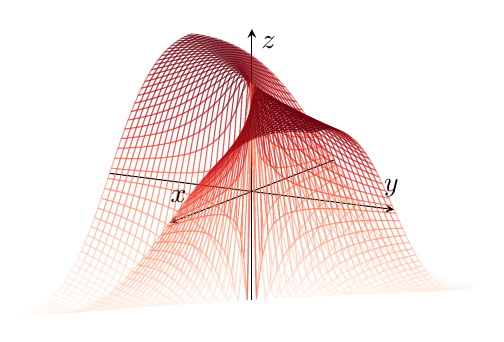
\begin{tikzpicture}
			\begin{axis}[
			view={120}{15},
			axis lines=middle,
			axis line style=black,
			xlabel={$x$},
			xtick={0},
			xmin=-1,xmax=1,
			ylabel={$y$},
			ytick={0},
			ymin=-1,ymax=1,
			zlabel={$z$},
			ztick={0},
			zmin=-0.5,zmax=0.75,
			width=0.6\textwidth,
			]
			\addplot3[mesh,samples=50,domain=-1:1,
			colormap/Reds,opacity=0.5]{x*y/(x^2+y^2)};
			\end{axis}
			\end{tikzpicture}
			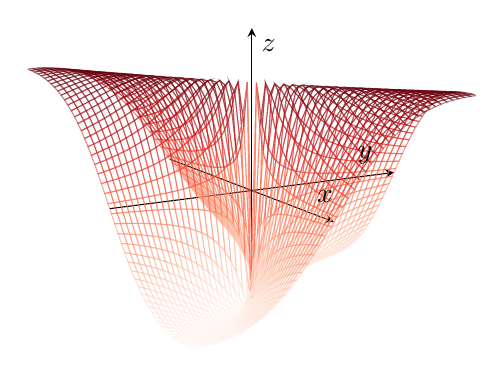
\begin{tikzpicture}
			\begin{axis}[
			view={60}{15},
			axis lines=middle,
			axis line style=black,
			xlabel={$x$},
			xtick={0},
			xmin=-1,xmax=1,
			ylabel={$y$},
			ytick={0},
			ymin=-1,ymax=1,
			zlabel={$z$},
			ztick={0},
			zmin=-0.5,zmax=0.75,
			width=0.6\textwidth,
			]
			\addplot3[mesh,samples=50,domain=-1:1,
			colormap/Reds,opacity=0.5]{x*y/(x^2+y^2)};
			\end{axis}
			\end{tikzpicture}
		\end{center}
		\caption{Two views of the graph of the function $f$ from \cref{partials-dont-imply-differentiable}. The one on the left is obtained from the one on the right by a 90$^\circ$ rotation counterclockwise around the $z$-axis.} \label{partials-dont-imply-differentiable-graph}
	\end{figure}
\end{exercise}

\begin{exercise} \label{directionals-dont-imply-differentiable}
	Consider the function $f : \R^2 \to \R$ given by
	\[ f(x,y) = \begin{cases} \dfrac{x^3}{x^2 +y^2} & \text{if } (x, y) \neq 0 \\ 0 & \text{if } (x,y) = 0. \end{cases} \]
	See \cref{directionals-dont-imply-differentiable-graph}.
	\begin{figure}[ht]
		\begin{center}
			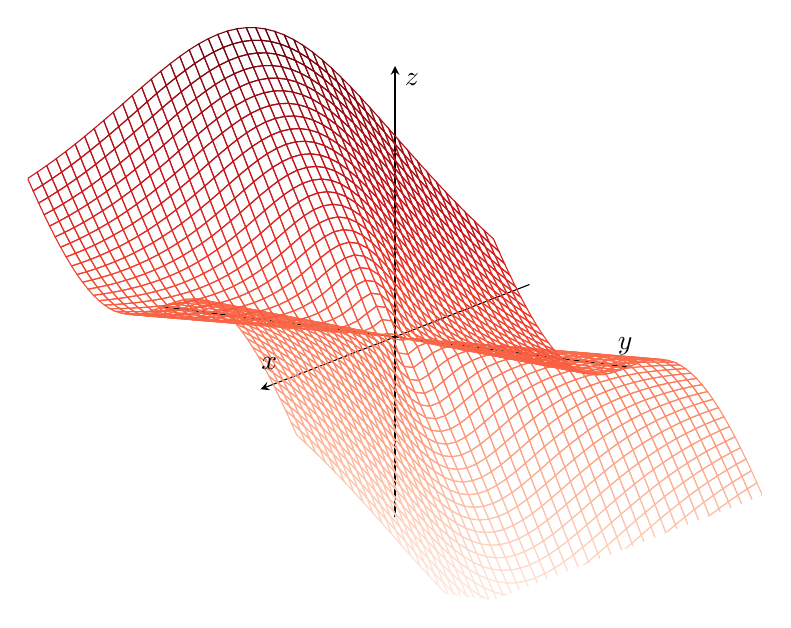
\begin{tikzpicture}
			\begin{axis}[
			view={120}{15},
			axis lines=middle,
			xlabel={$x$},
			xtick={0},
			xmin=-1,xmax=1,
			ylabel={$y$},
			ytick={0},
			ymin=-1,ymax=1,
			zlabel={$z$},
			ztick={0},
			zmin=-0.5,zmax=0.75,
			width=0.9\textwidth,
			]
			\addplot3[mesh,samples=50,domain=-1:1,
			colormap/Reds]{x^3/(x^2+y^2)};
			\end{axis}
			\end{tikzpicture}
		\end{center}
		\caption{The graph of the function  $f$ from \cref{directionals-dont-imply-differentiable}.} \label{directionals-dont-imply-differentiable-graph}
	\end{figure} 
	\begin{enumerate}[(a)]
		\item Show that $f$ is continuous. 
		\item Show that $\partial_{(h,k)} f(0)$ exists for all nonzero $(h,k) \in \R^2$, but that $f$ is not differentiable at the origin.
		\begin{hint}
			Calculate a formula for $\partial_{(h,k)} f(0)$ for all $(h,k) \in \R^2$, and show that the function $\R^2 \to \R$ given by $(h,k) \mapsto \partial_{(h,k)} f(0)$ is not linear. Explain why \cref{differentiable-implies-directionals} then implies that $f$ is \emph{not} differentiable at 0.  
		\end{hint}
		\item Suppose that $\gamma : \R \to \R^2$ is differentiable at 0, that $\gamma(0) = 0$, and that $d\gamma_0 \neq 0$. Show that $f \circ \gamma$ is differentiable at 0. 
	\end{enumerate} 
\end{exercise}

\begin{exercise} \label{directionals-and-linear-dont-imply-differentiable}
	Consider the function $f : \R^2 \to \R$ given by
	\[ f(x,y) = \begin{cases} |x| & \text{if } y = x^2 \\ 0 & \text{otherwise}. \end{cases} \]
	\begin{enumerate}[(a)]
		\item Sketch a graph of $f$ by hand.
		\item Show that $f$ is continuous at the origin. 
		\item Show that all directional derivatives of $f$ at the origin exist and are equal to 0. 
		\begin{hint}
			First show it for the partial derivatives, using \cref{directional-to-single}. Then fix $r \neq 0$ and show that $\partial_{(1,r)}f(0) = 0$, again using \cref{directional-to-single}. Then use \cref{basic-directional-derivative-properties} to conclude. 
		\end{hint}
		\item Show that $f$ is not differentiable at the origin.
		\begin{hint}
			Find a differentiable function $\gamma : \R \to \R^2$ such that $\gamma(0) = 0$ and $f \circ \gamma$ is not differentiable at the origin, and then use the chain rule \ref{chain-rule} to conclude that $f$ cannot be differentiable at the origin. 
		\end{hint}
	\end{enumerate} 
\end{exercise}

Thankfully, the failure of partial derivatives to imply differentiability is relatively pathological. \Cref{continuous-partials} below proves that the partial derivatives existing \emph{and being continuous} is sufficient to guarantee differentiability. 

% TODO: Derivatives along curves

\subsection{Jacobian matrix}

\begin{definition}[Jacobian matrix]  \index{jacobian matrix}
	Suppose $f : S \to \R^n$ is differentiable at an interior point $a \in S$. The \emph{Jacobian matrix} of $f$ at $a$, denoted $f'(a)$, is the $n \times m$ matrix whose $(j, i)$-entry is $\partial_i f_j(a)$. In other words,
	\[ f'(a) = \begin{bmatrix} \partial_1 f_1(a) & \partial_2 f_1(a) & \dotsb & \partial_m f_1(a) \\ 
	\partial_1 f_2(a) & \partial_2 f_2(a) & \dotsb & \partial_m f_2(a) \\
	\vdots & \vdots & \ddots & \vdots \\ 
	\partial_1 f_n(a) & \partial_2 f_n(a) & \dotsb & \partial_m f_n(a) \end{bmatrix} \]
	Note that \cref{differentiable-by-components,differentiable-implies-directionals} tell us that all of these partial derivatives exist. 
\end{definition}

\begin{theorem} \label{jacobian-matrix}
	If $f : S \to \R^n$ is differentiable at an interior point $a \in S$, then \[ df_a(h) = \begin{bmatrix} \partial_h f_1(a) \\ \cdots \\ \partial_h f_n(a) \end{bmatrix}. \]
	In particular, $[df_a] = f'(a)$. 
\end{theorem}

\begin{exercise}
	Prove \cref{jacobian-matrix}. \begin{hint} Use \cref{differentiable-by-components,differentiable-implies-directionals}. \end{hint}
\end{exercise}

Using \cref{jacobian-matrix}, many of the rules for differentiation we've seen can be rewritten in forms that you might be more familiar with from single variable calculus. For example, since composition of linear maps corresponds to multiplication of the corresponding matrix representations, the chain rule \ref{chain-rule} states that 
\[ (g \circ f)'(a) = [d(g \circ f)_a] = [dg_{f(a)} \circ df_a] = [dg_{f(a)}] [df_a] = g'(f(a)) f'(a). \]
Though the equality $(g \circ f)'(a) = g'(f(a)) f'(a)$ looks superficially identical to the equality from the single variable chain rule \ref{chain-rule-single}, it's worth noticing that the terms in this multivariable version are \emph{matrices}. In particular, this means that that order of the multiplication $g'(f(a))f'(a)$ cannot be interchanged (this was a non-issue in the single variable case). 

Similarly, the matrix version of the multivariable product rule \ref{product-rule} states that 
\[ (fg)'(a) = g(a)f'(a) + f(a)g'(a), \]
which again looks superficially identical to the single variable product rule \ref{product-rule-single}, but again, it is worth noting that $g(a)$ and $f(a)$ are scalars, whereas $f'(a)$ and $g'(a)$ are matrices. 

\begin{unimportantremark}
	For a single variable function differentiable $f$, in \cref{single} we saw that the differential $df_a$ to be the linear map given by multiplication by the derivative $f'(a)$, and the derivative $f'(a)$ was the standard matrix representation $[df_a]$ of the differential $df_a$. For multivariable differentiable functions $f$, the differential $df_a$ is the linear map given by left multiplication by the Jacobian matrix $f'(a)$, and the Jacobian matrix $f'(a)$ is the standard matrix representation $[df_a]$ of the differential $df_a$. The term ``derivative'' is a little ambiguous for multivariable functions; sometimes people will use it to refer to the differential $df_a$, and sometimes people will use it to refer to the Jacobian matrix $f'(a)$. 
\end{unimportantremark}

\subsection{Rank of a differentiable map}

\begin{definition}[Rank of a differentiable map] \label{immersive-submersive-critical} \index{rank!of a differentiable function}
	Suppose $f : S \to \R^n$ is differentiable at an interior point $a \in S$. The rank of the differential $df_a : \R^m \to \R^n$ (or, equivalently, the rank of the Jacobian matrix $f'(a)$) is also called the \emph{rank of $f$ at $a$}, denoted $\rank_a(f)$. Note that we always have \[ \rank_a(f) \leq \min\{m,n\}. \]
	We then make the following definitions in various special cases. 
	\begin{itemize}
		\item We say that $f$ is \emph{immersive at $a$}\index{immersive} if $\rank_a(f) = m$ (equivalently, if $df_a$ is injective). 
		\item We say that $f$ is \emph{submersive at $a$}\index{submersive} if $\rank_a(f) = n$ (equivalently, if $df_a$ is surjective). 
		\item We say that $f$ is \emph{\'etale at $a$}\index{etale@\'etale} if $\rank_a(f) = m = n$ (equivalently, if $df_a$ is an isomorphism). 
		\item We say that $a$ is a \emph{regular point}\index{regular!regular point} of $f$ if $\rank_a(f) = \min\{m,n\}$. Otherwise, we say that $a$ is a \emph{critical point}\index{critical! critical point} of $f$.
	\end{itemize}
	We also say that a point $b \in \R^n$ is a \emph{regular value}\index{regular!regular value} of $f$ if every $a \in f^{-1}(b)$ is a regular point of $f$, and that it is a \emph{critical value}\index{critical!critical value} otherwise. 
\end{definition}

There are lots of relationships between these notions, depending on how the dimension of the domain, $m$, compares with the dimension of the codomain, $n$. You should convince yourself of the following facts.  
\begin{itemize}
	\item If $m > n$...
	\begin{itemize}
		\item $f$ cannot be immersive at any point.
		\item $a$ is a regular point of $f$ if and only if $f$ is submersive at $a$.
	\end{itemize}
	\item If $m < n$...
	\begin{itemize}
		\item $f$ cannot be submersive at any point.
		\item $a$ is a regular point of $f$ if and only if $f$ is immersive at $a$.
	\end{itemize}
	\item If $m = n$...
	\begin{itemize}
		\item $a$ is a regular point of $f$ if and only if $f$ is immersive at $a$, if and only if $f$ is submersive at $a$, if and only if $f$ is \'etale at $a$. 
	\end{itemize}
\end{itemize}

\begin{caution}
	Some mathematicians use a different definition of ``regular point.'' They define a point to be regular if $\rank_a(f) = n$, so that, by definition, it's \emph{always} true (for all $m, n$ regardless of how these two integers compare) that $f$ is a submersion at $a$ if and only if $a$ is a regular point of $f$. If $m \geq n$, there's no difference between these alternative definitions and our definitions. But, if $m < n$, there is a difference: these other mathematicians would say that all points are critical in this case, but that isn't true for us with the definitions we've made above. So, if you see the words ``regular point'' and ``critical point'' in another text and it's possible that $m < n$, it's worth looking back to make sure you know what the author means!
\end{caution}

\begin{unimportantremark}
	While we're on the topic of terminology, it may be worth mentioning that the word ``\'etale'' is not commonly used in real analysis or in differential geometry; in fact, as far as I'm aware, there is no word in these fields that means that the derivative is invertible. But the word ``\'etale'' is used in algebraic geometry to mean that the derivative is invertible, so I decided to import this word from algebraic geometry. That said, if you do go on to study algebraic geometry at some point, it's worth noting the algebraic geometry words corresponding to ``immersive'' and ``submersive'' are ``unramified'' and ``smooth,'' respectively. This usage of ``smooth'' in algebraic geometry is unrelated to the real analysis and differential geometry usage of smooth that we'll encounter later on. 
\end{unimportantremark}

\begin{example} \label{polar-map}

Let $f : \R^2 \to \R^2$ be the map $f(r,\theta) = (r\cos\theta, r\sin\theta)$. See \cref{polar-map-picture}. 
\begin{figure}
	\begin{center}
		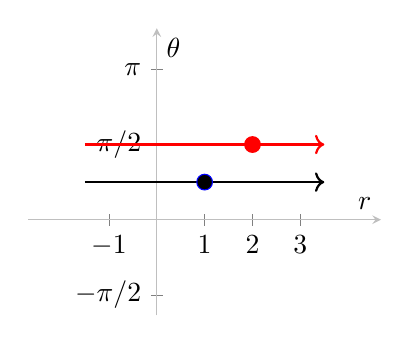
\begin{tikzpicture}
		\begin{axis}[
		xmin=-2,xmax=4,
		ymin=-2,ymax=4,
		ytick={-1.57,1.57,3.14},
		xtick={-1,1,2,3},
		yticklabels={$-\pi/2$,$\pi/2$, $\pi$},
		axis lines=middle,
		axis line style=lightgray,
		width=0.5\textwidth,
		xlabel={$r$},
		ylabel={$\theta$},
		axis equal
		] 
		
		\addplot[red,thick,->] expression[domain=-1.5:3.5,samples=2]{1.57};
		\node[color=red,draw=red,circle,fill,inner sep=2pt] at (axis cs:2,1.57) {}; 
		
		\addplot[black,thick,->] expression[domain=-1.5:3.5,samples=2]{1.57/2};
		\node[color=black,draw=blue,circle,fill,inner sep=2pt] at (axis cs:1,1.57/2) {}; 
		
		\end{axis}
		\end{tikzpicture}\hspace{1cm}
		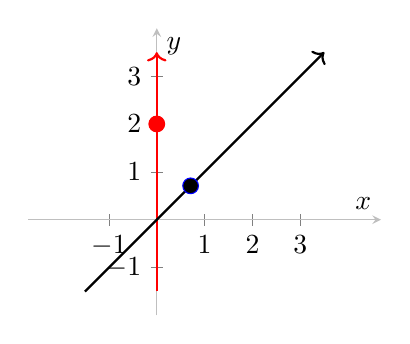
\begin{tikzpicture}
		\begin{axis}[
		xmin=-2,xmax=4,
		ymin=-2,ymax=4,
		ytick={-1,1,2,3},
		xtick={-1,1,2,3},
		axis lines=middle,
		axis line style=lightgray,
		width=0.5\textwidth,
		xlabel={$x$},
		ylabel={$y$},
		axis equal
		] 
		
		\addplot +[mark=none,red,thick,->] coordinates {(0, -1.5) (0, 3.5)};
		\node[color=red,draw=red,circle,fill,inner sep=2pt] at (axis cs:0,2) {}; 
		
		\addplot[black,thick,->] expression[domain=-1.5:3.5,samples=2]{x};
		\node[color=black,draw=blue,circle,fill,inner sep=2pt] at (axis cs:0.707,0.707) {}; 
		\end{axis}
		\end{tikzpicture}
		
		\mbox{}
		
		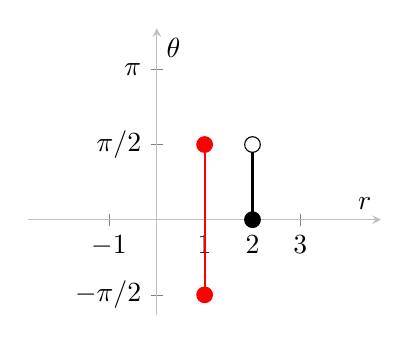
\begin{tikzpicture}
		\begin{axis}[
		xmin=-2,xmax=4,
		ymin=-2,ymax=4,
		ytick={-1.57,1.57,3.14},
		xtick={-1,1,2,3},
		yticklabels={$-\pi/2$,$\pi/2$, $\pi$},
		axis lines=middle,
		axis line style=lightgray,
		width=0.5\textwidth,
		xlabel={$r$},
		ylabel={$\theta$},
		axis equal
		] 
		
		\addplot +[mark=none,red,thick] coordinates {(1, -1.57) (1,1.57)};
		\node[color=red,draw=red,circle,fill,inner sep=2pt] at (axis cs:1,-1.57) {}; 
		\node[color=red,draw=red,circle,fill,inner sep=2pt] at (axis cs:1,1.57) {}; 
		
		\addplot +[mark=none,black,thick] coordinates {(2, 0) (2,1.57)};
		\node[color=black,draw=black,circle,fill,inner sep=2pt] at (axis cs:2,0) {}; 
		\node[color=white,draw=black,circle,fill,inner sep=2pt] at (axis cs:2,1.57) {}; 
		
		\end{axis}
		\end{tikzpicture}\hspace{1cm}
		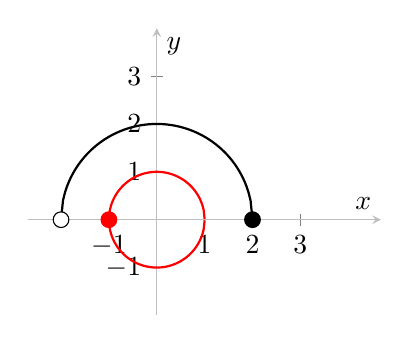
\begin{tikzpicture}
		\begin{axis}[
		xmin=-2,xmax=4,
		ymin=-2,ymax=4,
		ytick={-1,1,2,3},
		xtick={-1,1,2,3},
		axis lines=middle,
		axis line style=lightgray,
		width=0.5\textwidth,
		xlabel={$x$},
		ylabel={$y$},
		axis equal
		] 
		
		\addplot[red,thick] expression[domain=-1:1,samples=100]{sqrt(1-x^2)}; 
		\addplot[red,thick] expression[domain=-1:1,samples=100]{-sqrt(1-x^2)}; 
		\node[color=red,draw=red,circle,fill,inner sep=2pt] at (axis cs:-1,0) {}; 
		
		\addplot[black,thick] expression[domain=-2:2,samples=100]{sqrt(4-x^2)}; 
		\node[color=black,draw=black,circle,fill,inner sep=2pt] at (axis cs:2,0) {}; 
		\node[color=white,draw=black,circle,fill,inner sep=2pt] at (axis cs:-2,0) {}; 
		\end{axis}
		\end{tikzpicture}
	\end{center}
	\caption{The function $f(r, \theta) = (r\cos\theta, r\sin\theta)$ of \cref{polar-map} transforms the pictures on the right to the pictures on the left.}  \label{polar-map-picture}
\end{figure}

We compute partial derivatives. 
\[ \frac{\partial f_1}{\partial r} = \cos \theta \quad \frac{\partial f_2}{\partial r} = \sin \theta \quad \frac{\partial f_1}{\partial \theta} = -r\sin \theta \quad \frac{\partial f_2}{\partial \theta} = r\cos \theta.  \]
Thus
\[ f'(r, \theta) = \begin{bmatrix} \cos \theta & -r \sin \theta \\ \sin \theta & r \cos \theta \end{bmatrix}. \]
Since this is a square matrix, $df_{(r, \theta)}$ has non-maximal rank if and only if its determinant vanishes. But
\[ \det f'(r, \theta) = r\cos^2 \theta + r\sin^2 \theta = r, \]
so the critical locus\index{critical point!critical locus} (ie, the set of all critical points) of $f$ is the vertical line $r = 0$, and $f$ is \'etale away from this line. 
\end{example}

\begin{exercise}[Fold] \label{fold}
	Let $f : \R^2 \to \R^2$ be the function given by $f(x, y) = (x, y^2)$. 
	\begin{enumerate}[(a)]
		\item Draw pictures of $f$ (like the pictures in \cref{polar-map} above) until you can see why this function is called a ``fold.''
		\item What is the critical locus of $f$? 
	\end{enumerate}
\end{exercise}

\begin{exercise}[Parametrization of a cusp] \label{cusp}
	Consider the function $f : \R \to \R^2$ defined by
	\[ f(t) = (t^2, t^3). \]
	See \cref{cusp-graph} for a picture of the image of $f$. The ``pointy'' part at the origin is sometimes called a cusp\index{cusp}.
	\begin{figure}
			\begin{center}
			\begin{tikzpicture}
			\begin{axis}[
			xmin=-0.5,xmax=2,
			ymin=-2,ymax=2,
			ytick={0},
			xtick={0},
			xticklabels={},
			yticklabels={},
			axis lines=middle,
			axis line style=lightgray,
			width=0.75\textwidth
			]
			\addplot[black,style=thick,->] expression[domain=0:1.5,samples=50]{ sqrt(x^3) };
			\addplot[black,style=thick,-] expression[domain=0:1.5,samples=50]{ -sqrt(x^3) }; 
			\node[color=black,draw=black,circle,fill,inner sep=2pt] at (axis cs:0,0) {}; 
			
			\end{axis}
			\end{tikzpicture}
		\end{center}
	\caption{The image of the function $f(t) = (t^2, t^3)$. The origin is $f(0)$.}  \label{cusp-graph}
	\end{figure}
	Calculate $f'(t)$ for all $t \in \R$. Show that 0 is a critical point of $f$, and that $f$ is immersive away from 0.
\end{exercise}


\begin{exercise}[Parametrization of a node] \label{node}
	Consider the function $f : \R \to \R^2$ defined by
	\[ f(t) = (t^2-1, t^3-t). \]
	See \cref{node-graph} for a picture of the image of $f$. The self-intersecting part at the origin is called a node\index{node}. 
	\begin{figure}
		\begin{center}
			\begin{tikzpicture}
			\begin{axis}[
			xmin=-1.5,xmax=1,
			ymin=-1.5,ymax=1.5,
			ytick={0},
			xtick={},
			xticklabels={},
			yticklabels={},
			axis lines=middle,
			axis line style=lightgray,
			width=0.75\textwidth
			]
			\addplot[black,style=thick,->] expression[domain=-1:0.9,samples=500]{ sqrt(x^2*(x+1)) };
			\addplot[black,style=thick,-] expression[domain=-1:0.9,samples=500]{ - sqrt(x^2*(x+1)) }; 
			\node[label={$f(\pm1)$},color=black,draw=black,circle,fill,inner sep=2pt] at (axis cs:0,0) {}; 
			\node[label={120:$f(0)$},color=black,draw=black,circle,fill,inner sep=2pt] at (axis cs:-1,0) {}; 
			
			\end{axis}
			\end{tikzpicture}
		\end{center}
		\caption{The image of the function $f(t) = (t^2-1, t^3-t)$. We have $f(0) = (-1,0)$ and $f(\pm 1) = (0,0)$.}  \label{node-graph}
	\end{figure}
	Calculate $f'(t)$ for all $t \in \R$, and show that $f$ is immersive everywhere.
\end{exercise}

\begin{exercise}
	Show that an interior point $a \in S$ is a critical point\index{critical point} of $f : S \to \R$ if and only if $\partial_i f(a) = 0$ for all $i$. 
\end{exercise}

\begin{exercise} \label{sphere-fibration}
	Let $f : \R^3 \to \R$ be the function
	\[ f(x,y,z) = x^2 + y^2 + z^2 \]
	Calculate $f'(a)$ for all $a \in \R^3$, and find all critical points of $f$. Also, describe the level sets of $f$. In other words, for fixed $r \in \R$, describe the set of all $a \in \R^3$ such that $f(a) = r$. 
\end{exercise}

\begin{exercise}
	Find the critical points of the function $f : \R^3 \to \R^2$ given by \[ f(x,y,z) = (xy, z). \]
\end{exercise}

\begin{exercise}
	Find the critical points of the function $f : \R^3 \to \R^2$ given by \[ f(x,y,z) = (x+y^2, y+z^2). \]
\end{exercise}

\section{Differentiable functions}

We saw in \cref{differentiable-at-a-point-but-not-in-any-neighborhood} that a function that is differentiable at a point need not be differentiable at nearby points. Functions which are differentiable throughout an open set have some nice properties, which we discuss in this section. Throughout this section, $U$ denotes an open subset of $\R^m$. 

\begin{definition} \index{differentiable} \index{derivative}
	A function $f : U \to \R^n$ is \emph{differentiable} if it is differentiable at every $a \in U$. The \emph{differential} or the \emph{total derivative} of $f$, denoted $df$, is the function $U \to \mathscr{L}(\R^m, \R^n)$ given by $a \mapsto df_a$, where $\mathscr{L}(\R^m, \R^n)$ denotes the set of all linear maps $\R^m \to \R^n$.  
\end{definition}

\begin{definition}
	If $f : U \to \R$ and $h \in \R^m$ is a vector such that $\partial_h f(a)$ exists for all $a \in U$, then the \emph{directional derivative} of $f$ with respect to $h$ is the function $\partial_h f$ given by $a \mapsto \partial_h f(a)$. When $h = e_i$ is one of the standard basis vectors, this function is called the \emph{$i$th partial derivative} of $f$ and is denoted $\partial_i f$. If we're using the variable $x_i$ to denote the $i$th component of the input of $f$, then $\partial_i f$ is sometimes also denoted by one of the following. 
	\[ f_{x_i} \quad \frac{\partial f}{\partial x_i} \]
\end{definition}

\subsection{Convex subsets}

Recall that, in the single variable situation of \cref{single-differentiable}, a key role was played by functions defined on intervals. In the multivariable situation, a similar role is played by functions defined on ``convex'' subsets. These are subsets $S \subseteq \R^m$ such that any two points in $S$ can be joined by a straight line segment that never leaves $S$. 

\begin{definition} \label{straight-line-path}
	If $a, b \in \R^m$, the \emph{straight line path} from $a$ to $b$ is the function
	\[ \gamma(t) = (1-t)a + tb. \]
	Observe that $\gamma(0) = a$ and $\gamma(1) = b$. 
\end{definition}

\begin{exercise} \label{straight-line-path-differentiable}
	Show that, for any $a, b \in \R^m$, the straight line path from $a$ to $b$ is differentiable. 
\end{exercise}

\begin{definition} \label{convex}
	A subset $S$ of $\R^m$ is said to be \emph{convex} if, whenever $a, b \in S$ and $\gamma$ is the straight line path from $a$ to $b$, then $\gamma(t) \in S$ for all $t \in [0,1]$. 
\end{definition}

\begin{exercise}
	Determine whether or not
	\[ S = \{ (x, y) \in \R^2 : x \geq 0 \text{ or } y \neq 0 \} \]
	is a convex subset of $\R^2$. Justify your answer. 
\end{exercise}

\begin{exercise}
	Let $I$ be an interval. Suppose $f : I \to \R$ is concave down and $f \geq 0$. Show that
	\[ S = \{ (x, y) \in \R^2 : x \in I \text{ and } 0 \leq y \leq f(x) \} \]
	is a convex subset of $\R^2$. 
\end{exercise}

\subsection{Vanishing derivatives}

Here is a multivariable generalization of \cref{constant-iff-derivative-zero-single}. We will use the single variable version to prove this multivariable version. 

\begin{proposition} \label{constant-iff-derivative-zero}
	Suppose $U$ is convex and $f : U \to \R^n$ is a differentiable function. Then $df = 0$ if and only if $f$ is constant\index{constant function}.  
\end{proposition}

\begin{proof}
	Taking $w = 0$ in \cref{derivative-of-line} shows that, if $f$ is constant, then $df = 0$. For the converse, we can assume without loss of generality that $n = 1$ (cf. \cref{constant-iff-derivative-zero-details}). We want to show that, for any $a,  b \in U$, we have $f(a) = f(b)$. Let $\gamma$ be the straight line path from $a$ to $b$. Convexity of $U$ tells us that $\gamma(t) \in U$ for all $t \in [0,1]$. Also, $\gamma$ is differentiable by \cref{straight-line-path-differentiable}. Thus $f \circ \gamma$ is a differentiable function $[0,1] \to \R$ and 
	\[ (f \circ \gamma)'(t) = f'(\gamma(t)) \gamma'(t) = 0 \]
	where we used the (matrix version of the) chain rule \ref{chain-rule} at the second step, and the fact that $df = 0$ for the final step. Thus it follows from \cref{constant-iff-derivative-zero-single} that $f \circ \gamma$ is constant, which means that
	\[ f(a) = f(\gamma(0)) = f(\gamma(1)) = f(b). \qedhere \]
\end{proof}

\begin{exercise} \label{constant-iff-derivative-zero-details}
	 Explain why proving that $df = 0$ implies that $f$ is constant for $n = 1$ implies the same fact for general $n$. 
\end{exercise}

In fact, it's not necessary that the domain be convex in order for the conclusion of \cref{constant-iff-derivative-zero} to be true. Before getting to the general statement, here is a useful intuition-building exercise. 

\begin{exercise}
	Let $U$ denote $\R^2$ minus the non-negative $x$-axis. In other words,
	\[ U = \R^2 \setminus \{ (x, 0) \in \R^2 : x \geq 0 \}. \]
	\begin{enumerate}[(a)]
		\item Show that $U$ is not convex. 
		\item Suppose $f : U \to \R$ is a differentiable function such that $df = 0$. Show that $f$ is constant.
	\end{enumerate} 
	\begin{hint}
		Any pair of points in $U$ \emph{can} be joined by \emph{two} straight line paths...
	\end{hint}
\end{exercise}

\begin{exercise} \label{constant-iff-derivative-zero-connected}
	Let $U$ be a connected\footnotemark\ open subset of $\R^m$.
	\begin{enumerate}[(a)]
		\item Show that, for any $a, b \in U$, there exists a finite sequence of points \[ a = a_0, a_1, \dotsc, a_k = b \] such that the image of the straight line path between $a_i$ and $a_{i+1}$ is entirely contained in $U$ for all $i$. 
		
		\begin{hint}
			For $a \in U$, consider the set $S$ of all points $a' \in U$ such that there exists a finite sequence of points $a = a_0, a_1, \dotsc, a_k = a'$ such that the image of the straight line path connecting $a_i$ to $a_{i+1}$ is entirely contained in $U$ for all $i$. Show that $S$ is open, and also that the complement of $S$ is open. Since $U$ is connected and $S$ is nonempty, it must be that the complement of $S$ is empty.  
		\end{hint}
		
		\item If $f : U \to \R^n$ is differentiable, show that $df = 0$ if and only if $f$ is constant. 
	\end{enumerate}
\end{exercise}

\footnotetext{Recall that a metric space $X$ is \emph{connected}\index{connected} if it cannot be written as the union of two disjoint open subsets.}

\subsection{Bounded derivatives}

Here is a multivariable version of \cref{bounded-derivative}. Again, we will actually use the single variable version to prove the multivariable version. 

\begin{proposition} \label{bounded-derivative-multi}
	Suppose $U$ is convex and $f : U \to \R^n$ is a differentiable function. Suppose further that there exists a constant $M$ such that $\|df_x\| \leq M$ for all $x \in U$. Then
	\[ |f(b) - f(a)| \leq M |b-a| \]
	for all $a, b \in U$. 
\end{proposition}

\begin{proof}
	Suppose first that $n = 1$. If $a = b$, there is nothing to do, so we can assume that $a \neq b$. Let \[ h = \frac{b-a}{|b-a|}, \]
	ie, $h$ is the vector pointing from $a$ towards $b$ normalized to unit length. Consider the function $\xi(t) = a + th$ as in \cref{directional-to-single}. Then
	\[ (f \circ \xi)'(t) = \partial_h f(a + th) = df_{a + th}(h)  \]
	by \cref{jacobian-matrix}, which means that 
	\[ |(f \circ \xi)'(t)| = |df_{a + th}(h)| \leq \|df_{a + th}\| |h| \leq M|h| = M, \]
	where we used the fact that $h$ has unit length for the final step. Notice that $\xi(0) = a$ and $\xi(|b-a|) =  b$, so by applying \cref{bounded-derivative} to $f \circ \xi$, we see that 
	\[ |f(b) - f(a)| \leq M||b-a| - 0| = M|b-a|.  \]
	This proves the statement for $n = 1$.
	
	We'll prove the statement for general $n$ only for the max norm and the max operator norm. The proof for the euclidean norm is trickier: see \cite[theorem 9.19]{rudin}. Note that $df_{j,a} = \pi_j \circ df_a$ and $\|\pi_j\|_\infty = 1$ so \[ \|df_{j,a}\|_\infty \leq \|\pi_j\|_\infty \|df_a\|_\infty \leq M \]
	by \cref{operator-norm-submultiplicative}. Applying \cref{bounded-derivative-multi} to the component functions $f_j$, we find that 
	\[ |f_j(b) - f_j(a)| \leq M|b-a| \]
	for all $a, b \in B$ and all $j = 1, \dotsc, n$. Taking the maximum over all $j$ proves the result. 
\end{proof}

\begin{exercise}
	\begin{enumerate}[(a)]
		\item The statement of the \cref{bounded-derivative-multi} requires that the domain of $f$ is convex. Where in the proof is this used?
		\item Prove that $\|\pi_j\|_2 = \|\pi_j\|_\infty = 1$. 
		\item If you haven't already done it, do \cref{operator-norm-submultiplicative}. 
	\end{enumerate} 
\end{exercise}

\subsection{Inverse function theorem}

The inverse function theorem is an extremely important foundational result. It comes up frequently in real analysis and differential geometry, and has inspired significant developments in algebraic geometry and number theory. 

\begin{definition}
	A differentiable function $f : U \to \R^n$ is \emph{\'etale} if it is \'etale at every $a \in U$ (ie, if $df_a$ is an isomorphism for every $a \in U$). 
\end{definition}

\begin{theorem}[Inverse function theorem] \label{inverse-function-theorem}
	Suppose $f : U \to \R^n$ is \'etale. Then $f$ is open. Moreover, for every $a \in U$, there exists an open neighborhood $V$ of $a$ such that $f|_V$ is injective, the inverse function $(f|_V)^{-1}$ is differentiable, and
	\[ d((f|_V)^{-1})_y = (df_{(f|_V)^{-1}(y)})^{-1} \]
	for all $y  \in f(V)$. 
\end{theorem}

The proof will require an extremely lengthy discussion. For the time being, let us content ourselves with thinking about the statement of the theorem. 

First off, let us compare the statement against the single variable version of \cref{inverse-function-theorem-single}. If $I$ is an open interval in $\R$, then $f : I \to \R$ is \'etale if and only if it is differentiable and $f'(x)$ never vanishes, so the hypotheses of the theorem above and the single variable version match up exactly. The multivariable version above asserts that $f$ must be open and ``locally injective.'' On the other hand, the single variable version asserts that $f$ is strictly monotone; and we've seen that strict monotonicity implies that $f$ is open and injective (cf. \cref{strictly-monotone-iff-injective,strictly-monotone-implies-open}). The assertion on the differentiability of the inverse and the formula for the derivative of the inverse match up exactly.  

Thus, the single variable version is a stronger statement (when it applies) because it guarantees full injectivity everywhere on the domain, whereas the multivariable version above only guarantees ``local injectivity'' near every point of the domain. This is the only difference between the two statements, and here is an example to show that we cannot expect full injectivity in the multivariable setting.  

\begin{exercise} \label{locally-injective-not-injective}
	Consider the function $f : \R^2 \to \R^2$ given by 
	\[ f(x,y) = (e^x \cos y, e^x \sin y). \]
	\begin{enumerate}[(a)]
		\item Compute $df$ and verify that $f$ is \'etale. 
		\item Show that $f$ is \emph{not} injective. In fact, for any point $(a,b)$ in the range, show that there exist infinitely many points in the domain which map to $(a,b)$.
		\item Find an open neighborhood $V$ of the origin such that $f|_V$ is injective. 
	\end{enumerate}
\end{exercise}

Another important observation about the statement is the following. The inverse function theorem asserts that being \'etale is \emph{sufficient} to guarantee the existence of (local) inverses. It is \emph{not} a necessary condition for the existence of inverses, but it \emph{is} a necessary condition for the existence of \emph{differentiable} inverses, as shown by the following exercise. 

\begin{exercise}
	\begin{enumerate}[(a)]
		\item Give an example of a differentiable and injective function $f : \R \to \R$ which is not \'etale. What is the inverse of your function $f$? Is the inverse differentiable? 
		\item Suppose $U$ is an open subset of $\R^n$ such that $f : U \to \R^n$ is differentiable and injective and that $f(U)$ is open. Show that, if $f^{-1} : f(U) \to \R^n$ is differentiable, then $f$ is \'etale.  
	\end{enumerate}
\end{exercise}

The importance of the inverse function theorem derives from the fact that it lets us use linear algebra (which is easy) to make assertions about solutions of nonlinear equations (which are very difficult, in general). Here is an example to illustrate this point. 

\begin{example}
	Consider the following nonlinear system of equations. 
	\[ \begin{aligned} x + x^2y &= a \\ y - xy^2 + 3x^2 &= b \end{aligned} \]
	When $a = b = 0$, this system has a solution given by $x = y = 0$. That much is clear. What if $a$ and $b$ are not both zero? Does this system have any solutions? Are the solutions unique at all? None of this is very obvious on the face of it. I at least do not see any clear way to solve for $x$ and $y$ in terms of $a$ and $b$.  
	
	Let $f : \R^2 \to \R^2$ be the function given by $f(x,y) = (x+x^2y, y - xy^2 + 3x^2)$. Then 
	\[ \det f'(x,y) = \det \begin{bmatrix} 1 + 2xy & x^2 \\ 6x -y^2 & 1 - 2xy \end{bmatrix} = 1 - 6x^3 - 3x^2y^2. \]
	This is a continuous function of $(x,y)$ and it is nonzero when $(x,y) = 0$, so there exists an open neighborhood $U$ of $0$ such that $\det f'(x,y) \neq 0$ for all $(x,y) \in U$. In other words, $f|_U$ is \'etale. By the inverse function theorem \ref{inverse-function-theorem}, we can replace $U$ with a smaller open neighborhood of 0 in order to guarantee that $f|_U$ is injective and open. Then $f(U)$ is an open neighborhood of $f(0) = 0$, and for every $(a,b) \in f(U)$, there exists a unique $(x,y) \in \R^2$ such that $f(x,y) = (a,b)$. 
	
	We have just proved that, for every $(a,b)$ in $f(U)$, the system has a unique solution given by $(x,y) \in U$. In other words, if we perturb $a$ and $b$ just a little bit away from 0, our system will have a unique solution close to 0. Thanks to the inverse function theorem \ref{inverse-function-theorem}, proving this boiled down to a simple linear algebra calculation!
\end{example}

Here are some more exercises and examples that may help clarify the statement of the inverse function theorem. 

\begin{exercise}
	Recall the function $f(x) = x + 2x^2 \sin(1/x)$ that we saw in \cref{positive-not-monotone}. As we've seen, $f'(0) = 1$ but $f$ is not monotone (hence not injective, by \cref{strictly-monotone-iff-injective}) on any open neighborhood of $0$. Explain why this does not violate the inverse function theorem. In other words, show that $f$ is not \'etale on any open neighborhood of 0.
\end{exercise}

\begin{exercise}
	Let $U = \{(x,y) \in \R^2 : x > 0\}$ and let $f : U \to \R^2$ be the function \[ f(x,y) = (xe^{-y}, xe^y). \]
	\begin{enumerate}[(a)]
		\item Show that $f$ is \'etale. 
		\item Show that $f$ is injective. What is $f(U)$?
		\item Calculate $(f^{-1})'(1,1)$. 
	\end{enumerate}
\end{exercise}

\subsection{Proof of the inverse function theorem \starred}

This section is devoted to the proof of the inverse function theorem \ref{inverse-function-theorem}. It's a long and arduous proof.

\subsubsection*{Differentiability of the local inverse}

As it turns out, once a local inverse has been constructed, proving that it is differentiable is not terribly difficult. The proof of this part is similar in spirit to the single variable version (cf. the proof of \cref{inverse-function-theorem-single}).

\begin{proposition} \label{inverse-differentiable}
	Suppose $f : U \to \R^n$ is differentiable, open, and injective. Then $f^{-1}$ is differentiable and \[ d(f^{-1})_y = (df_{f^{-1}(y)})^{-1} \] for all $y \in f(U)$. 
\end{proposition}

\begin{proof}
	Fix $x \in U$ and $y = f(x)$. Let
	\[ s(k) = f^{-1}(y + k) - f^{-1}(k) - df_x^{-1}(k). \]
	We want to show that $|s(k)| = o(|k|)$ as $k \to 0$. In fact, since $df_x$ is an invertible linear map, it is sufficient to show that $|df_x(s(k))| = o(|k|)$ (cf. \cref{chain-rule-details} part  (\ref{linear-of-small-is-small})). 
	
	Define \[ h(k) = f^{-1}(y + k) - f^{-1}(y). \]
	Since $f$ is injective, we see that $h(k) = 0$ if and only if $k = 0$. Moreover, $f^{-1}$ is continuous since $f$ is open, which implies that $h$ is also continuous. Now by rewriting $s$ in terms of $h$, we have the following. 
	\[ \begin{aligned} 
	s(k) &= h(k) - df_x^{-1}(k) \\
	df_x(s(k)) &= df_x(h(k)) - k \\
	&= df_x(h(k)) - y + k + y \\
	&= df_x(h(k)) - f(x+h(k)) + f(x). \end{aligned} \]
	In other words, if we consider the ``error in approximation'' function
	\[ r(h) = f(x+h) - f(x) - df_x(h), \]
	then
	\[ df_x(s(k)) = -r(h(k)) \]
	for all $k$. This means that, for all $k \neq 0$, we have
	\[ \frac{|df_x(s(k))|}{|k|} = \frac{|r(h(k))|}{|k|} = \frac{|r(h(k))|}{|h(k)|} \cdot \frac{|h(k)|}{|k|} \]
	where we have used the fact that $h(k) \neq 0$ since $k \neq 0$. Now, since $|r(h)| = o(|h|)$ as $h \to 0$ and since the function $h$ is continuous at $k = 0$, we have that 
	\[ \lim_{k \to 0} \frac{|r(h(k))|}{|h(k)|} = 0. \]
	Thus it is sufficient to show that there exists a constant $M$ such that $|h(k)| \leq M|k|$ for all sufficiently small values of $k$.
	
	Since $|r(h)| = o(|h|)$ as $h \to 0$, there exists $\delta > 0$ such that $|r(h)| \leq |h|$ for all $|h| < \delta$. Then we have 
	\[ \begin{aligned} |h| &\geq |r(h)| = |f(x+h) - f(x) - df_x(h)| \\ &\geq |df_x(h)| - |f(x+h) - f(a)| \\
	&\geq \frac{|h|}{\|df_x^{-1}\|} - |f(x+h)-f(x)| \end{aligned} \]
	where we have used \cref{operator-norm-inverse} for the final step. After rearranging, this becomes
	\[ |h| \leq \left(\frac{1}{\|df_x^{-1}\|} - 1\right)^{-1} |f(x+h) - f(x)|. \] 
	Set
	\[ M = \left(\frac{1}{\|df_x^{-1}\|} - 1\right)^{-1}. \]
	Now if $h = h(k)$, we have $f(x+h(k)) - f(x) = k$, so the last inequality displayed above reads
	\[ |h(k)| \leq M |f(x+h(k)) - f(x)| = M|k|. \qedhere \]
\end{proof}

\subsubsection*{Reductions}

For the remainder of this proof, $f : U \to \R^n$ will denote an \'etale map. In particular, this means that $m = n$, ie, that $U$ is an open subset of $\R^n$. We'll closely follow  \href{https://terrytao.wordpress.com/2011/09/12/the-inverse-function-theorem-for-everywhere-differentiable-maps/#more-5298}{Terry Tao's exposition} of Saint Raymond's proof \cite{saint-raymond}. 

Let's begin by making a couple of helpful definitions. 

\begin{definition}
	For any point $a \in U$, we make the following definitions. 
	\begin{itemize}
		\item We say that $f$ is \emph{locally injective at $a$} if there exists an open neighborhood $V$ of $a$ such that $f|_V$ is injective. 
		\item We say that $f$ is \emph{locally surjective at $a$} if $f(a)$ is an interior point of $f(V)$ for every open neighborhood $V$ of $a$. 
	\end{itemize}
\end{definition}

\begin{exercise} \label{open-iff-locally-surjective}
	Show that $f$ is open if and only if $f$ is locally surjective at every $a \in U$. 
\end{exercise}

\begin{solution}{\cref{open-iff-locally-surjective}}
	This is just unwinding definitions. Suppose $f$ is open. Fix a point $a \in U$ and let $V$ be an open neighborhood of $a$ in $U$. Since $f$ is open, $f(V)$ is open, so $f(a)$ must be an interior point of $f(V)$. Conversely, suppose $f$ is locally surjective at every point in $U$. Let $V$ be an open subset of $U$. If $b \in f(V)$, there is an $a \in V$ such that $f(a) = b$. But $f$ is locally surjective at $a$, so $f(a) = b$ is an interior point of $f(V)$. Thus every $b \in f(V)$ is an interior point of $f(V)$, so $f(V)$ is open. 
\end{solution}

In other words, to prove the inverse function theorem, we want to show that $f$ is locally injective and locally surjective at every point $a \in U$. We can replace $f$ with the function $x \mapsto f(x+a)$ in order to assume that $a = 0$. Then, we can replace $f$ with the function $x \mapsto f(x) - f(0)$ in order to assume that $f(0) = 0$. Finally, since $df_0$ is invertible, we can replace $f$ with $df_0^{-1} \circ f$ in order to assume that $df_0 = \id$. 

\begin{exercise} \label{wlog-inverse-function-theorem}
	Check that you understand the ``we can assume''s in the previous paragraph. More precisely, suppose $a \in U$, $\ell : \R^n \to \R^n$ is a linear map, $\alpha_0 \in \R^n$, and $\alpha : \R^n \to \R^n$ is the function \[ \alpha(x) = \ell(x) + \alpha_0. \]
	Prove the following facts. 
	\begin{enumerate}[(a)]
		\item Show that $\alpha$ is bijective, and calculate $d\alpha$ and $d\alpha^{-1}$. 
		\item Let $\tilde{f} = \alpha \circ f$. 
		\begin{itemize}
			\item Show that $f$ is \'etale if and only if $\tilde{f}$ is \'etale. 
			\item Show that $f$ is locally injective at $a$ if and only if $\tilde{f}$ is locally injective at $a$. 
			\item Show that $f$ is locally surjective at $a$ if and only if $\tilde{f}$ is locally surjective at $a$.
		\end{itemize}  
		\item Let $\tilde{f} : \alpha^{-1}(U) \to \R^n$ be the composite $\tilde{f} = f \circ \alpha$. 
			\begin{itemize}
				\item Show that $f$ is \'etale if and only if $\tilde{f}$ is \'etale. 
				\item Show that $f$ is locally injective at $a$ if and only if $\tilde{f}$ is locally injective at $\alpha^{-1}(a)$. 
				\item Show that $f$ is locally surjective at $a$ if and only if $\tilde{f}$ is locally surjective at $\alpha^{-1}(a)$.
			\end{itemize} 
		\item Figure out what $\ell$ and $\alpha_0$ are for each of the ``we can assume''s of the previous paragraph. 
	\end{enumerate}
\end{exercise}

In other words, we want to show that, if $f$ is an \'etale map such that $f(0) = 0$ and $df_0 = \id$, then $f$ is locally injective and locally surjective at 0. Local surjectivity is easier; local injectivity is very, very difficult. 

\subsubsection*{Local surjectivity}

Since $f(0) = 0$ and $df_0 = \id$, we have $|f(h) - h| = o(|h|)$ as $h \to 0$ by the definition of the derivative, so there exists $\delta > 0$ such that 
\begin{equation} \label{inverse-function-theorem-eqn1} |f(h)-h| \leq |h|/2 \end{equation}
for all $|h| < \delta$. Replacing $f$ with the function $x \mapsto f(x/\delta)$, we can assume without loss of generality that $\delta = 1$ (cf. \cref{wlog-inverse-function-theorem}). We now claim that for all $0 < r < 1$, we have
\begin{equation} \label{inverse-function-theorem-locally-surjective} B(0,r/3) \subseteq f(B(0,r)). \end{equation}
Suppose $b \in B(0, r/3)$. Let $\nu : \R^m \to \R$ be the differentiable function given by $\nu(x) = x_1^2 + \dotsb x_n^2$ and then consider the function $\sigma : \overline{B}(0,r) \to \R$ given by \[ \sigma(x) = \nu(f(x)-b). \]
Since $\overline{B}(0,r)$ is compact, this function must attain its minimum at a point $a \in \overline{B}(0,r)$. We will show that $a \in B(0,r)$ and that $f(a) = b$, thus proving \cref{inverse-function-theorem-locally-surjective}. 

First of all, we must have $a \in B(0,r)$. Suppose for a contradiction that $|a| = r$. Then by \cref{inverse-function-theorem-eqn1} we would have
\[ r/2 \geq |f(a)-a| \geq |a| - |f(a)| = r - |f(a)| > 2r/3, \]
where we've used the reverse triangle inequality for the second step. This is evidently contradiction, since $r/2 < 2r/3$. In other words, we have proved that $a$ is an interior point of the domain of $\sigma$. 

Now we prove that $f(a) = b$. The chain rule \ref{chain-rule} tells us that 
\[ d\sigma_{a} = d\nu_{f(a)-b} \circ df_{a}. \]
Since the interior point $a$ is the absolute minimum of $\sigma$, the interior extremum theorem \ref{interior-extremum-directional} and \cref{jacobian-matrix} tells us that $d\sigma_a = 0$, which means that $df_a(\R^n) \subseteq \ker(d\nu_{f(a)-b})$. Since $df_a$ is invertible, this means that $d\nu_{f(a)-b} = 0$. But we have 
\[ \nu'(x) = \begin{bmatrix} 2x_1 & 2x_2 & \dotsb & 2x_n \end{bmatrix} \]
so $d\nu_{f(a) - b} = 0$ if and only if $f(a) - b = 0$. We have now proved \cref{inverse-function-theorem-locally-surjective}. 

Notice that \cref{inverse-function-theorem-locally-surjective} implies that $f$ is locally surjective at 0. Indeed, any open neighborhood $V$ of 0 contains an open ball of the form $B(0,r)$ for $0 < r < 1$, and then \[ f(V) \supseteq f(B(0,r)) \supseteq B(0,r/3), \] so $f(0) = 0$ is an interior point of $f(V)$. 

\subsubsection*{Local injectivity under assumptions}

Proving local injectivity in general is very challenging, but is a bit easier if we add some hypotheses to the statement of the theorem. In this section, we look at some of these arguments under additional assumptions. 

\mbox{}

\noindent \textit{Assuming $n = 1$.} As we've already noted, we've already proved not just local injectivity but full injectivity when $n = 1$ in \cref{inverse-function-theorem-single}. In any case, it's worth isolating the argument of injectivity and inspecting it closely. 

Suppose we have $a_1 < a_2$ such that $f(a_1) = f(a_2)$. We'll prove that this leads to a contradiction using two different but very similar arguments. The first argument is very quick. The mean value theorem guarantees that there exists $\xi$ between $a_1$ and $a_2$ such that $f'(\xi) = 0$, which contradicts our assumption that $f$ is \'etale. 

The second argument avoids using the mean value theorem basically by proving the mean value theorem for this particular situation. The idea is to set $b := f(a_1) = f(a_2)$ and consider the function \[ \sigma(x) = (f(x)-b)^2. \]
Since $\sigma$ is a continuous function on the compact interval $[a_1, a_2]$, the extreme value theorem guarantees that it attains its maximum at some point $\xi \in [a_1, a_2]$. Observe that $\sigma(a_1) = \sigma(a_2) = 0$ and $\sigma \geq 0$, so if $\sigma(\xi) = 0$, then $\sigma = 0$ constantly, so $f$ is constantly equal to $b$, which means the derivative vanishes on $(a_1, a_2)$ by \cref{constant-iff-derivative-zero}, contradicting our assumption that $f$ is \'etale. Thus $\sigma(\xi)$ must be an interior point of the interval $(a_1, a_2)$ and $\sigma(\xi) \neq 0$, ie, $f(\xi) \neq b$. Then the interior extremum theorem \ref{interior-extremum} plus the chain rule tells us that
\[ 0 = \sigma'(\xi) = 2(f(\xi) - b)f'(\xi).  \]
Since $f(\xi) \neq b$, this says that $f'(\xi) = 0$, which again contradicts our assumption that $f$ is \'etale. 

This second argument is useful because the proof in the general setting involves maximizing a multivariable function that's very similar to the single variable function $\sigma$ above. But before we get to the general proof, here is another proof under additional hypotheses. 

\mbox{}

\noindent \textit{Assuming continuous differentiability.} We haven't formally defined it yet, but $f$ is said to be ``continuously differentiable'' if all of the partial derivatives of the component functions $\partial_i f_j$ are continuous (cf. \cref{continuously-differentiable-definition}). The proof that $f$ is locally injective at 0 is a little easier if we assume that $f$ is continuously differentiable, but still a little tricky. The proof here is essentially the one from \cite[chapter 2]{spivak_calculus}. 

Since $df_0 = \id$, we know that $\partial_i f_j(0) = \delta_{i,j}$. Since $\partial_i f_j$ is continuous at 0, there exists $\delta > 0$ such that 
\[ |\partial_i f_j(0) - \partial_i f_j(x)| = |\delta_{i,j} - \partial_i f_j(x)| \leq \frac{1}{2n}. \]
Let $V = B(0,\delta)$. We will show that $f|_V$ is injective. 

Let $g(x) = x - f(x)$. It turns out that it is sufficient to prove that $\|dg_x\| \leq 1/2$ for all $x \in V$. Indeed, if we can prove this, then \cref{bounded-derivative-multi} would tell us that 
\[ |g(x_1) - g(x_2)| \leq \frac{1}{2} |x_1 - x_2| \]
for all $x_1, x_2 \in V$. But
\[ |g(x_1) - g(x_2)| = |(x_1 - f(x_1)) - (x_2 - f(x_2))| \geq |x_1 - x_2| - |f(x_1) - f(x_2)| \]
by the reverse triangle inequality. This leads to the following. 
\[ \begin{aligned} |x_1 - x_2| - |f(x_1) - f(x_2)| &\leq \frac{1}{2} |x_1 - x_2| \\
\frac{1}{2}|x_1 - x_2| &\leq |f(x_1) - f(x_2)| \\
|x_1 - x_2| &\leq 2|f(x_1) - f(x_2)| \end{aligned} \]
This shows that $f(x_1) = f(x_2)$ if and only if $x_1 = x_2$, or, in other words, that $f|_V$ is injective. 

We'll prove that $\|df_x\| \leq 1/2$ only for the max norm (and, correspondingly, the max operator norm). Observe that $\partial_i g_j(x) = \delta_{i,j} - \partial_i f_j(x)$, so we have 
\[ |g'(x)|_\infty = \max_{i,j} |\partial_i g_j(x)| \leq \frac{1}{2n} \]
for all $x \in V$. Using \cref{max-matrix-norm-and-max-operator-norm}, we see that $\|dg_x\|_\infty \leq 1/2$ for all $x \in V$. 

\begin{unimportantremark}
	It is also true that $\|dg_x\|_2 \leq 1/2$. To prove this, we would use the fact that $\|\ell\|_2 \leq \sqrt{mn}|A|_\infty$ when $A$ is the standard matrix representation of a linear map $\ell : \R^m \to  \R^n$ (cf. \cite[section 2.3.2]{golub}), instead of \cref{max-matrix-norm-and-max-operator-norm}. In any case, we didn't prove \cref{bounded-derivative-multi} for the eucldiean norm situation, so perhaps its better to stick with the max norm here anyway. 
\end{unimportantremark}

\subsubsection*{Local injectivity}
	
{\color{blue} Incomplete. I'll write this up eventually. The continuously differentiable case we proved above is really sufficient almost all of the time (and is all we'll use as we go forward), but if you're really curious about the general case, look at \href{https://terrytao.wordpress.com/2011/09/12/the-inverse-function-theorem-for-everywhere-differentiable-maps/#more-5298}{Terry Tao's blog post}.}
% TODO: Local injecticity for inverse function theorem

% TODO: Implicit function theorem

\section{\texorpdfstring{$C^k$}{Ck} hierarchy}

Throughout this section, $U$ denotes an open subset of $\R^m$.

\subsection{Continuous differentiability}

\subsubsection*{Continuity of partials}

The following theorem is the promised sort-of-converse to \cref{differentiable-implies-directionals}. Recall from \cref{partials-dont-imply-differentiable} above that the partial derivatives all existing everywhere is \emph{not} sufficient to guarantee differentiability. But, insisting that the partial derivatives all exist \emph{and are continuous} turns out to be enough to guarantee differentiability of $f$. The proof is harder than you might expect. 

\begin{theorem} \label{continuous-partials}
	Suppose $f : U \to \R$ is a function such that the $i$th partial derivative $\partial_i f : U \to \R$ exists for all $i = 1 , \dotsc m$. If $a \in U$ is a point such that $\partial_i f$ is continuous at $a$ for all $i$, then $f$ is differentiable at $a$. 
\end{theorem}

\begin{proof}[Proof]
	If $f$ is to be differentiable at $a$, we know from \cref{jacobian-matrix} what $df_a$ needs to be in terms of the partial derivatives; so let's turn this on its head by writing down the linear map defined by the partial derivatives, and then proving that that linear map is in fact $df_a$. 
	
	More precisely, we mean the following. Let $\ell$ be the linear map $\R^m \to \R$ such that \[ [\ell] = \begin{bmatrix}
	\partial_1f(a) & \dotsb & \partial_m f(a)
	\end{bmatrix}. \]
	In other words, $\ell : \R^m \to \R$ is the linear map given by
	\[ \ell(h_1, \dotsc, h_m) = h_1 \partial_1 f(a) + \dotsb + h_m \partial_m f(a). \]
	We will show that 
	\[ |f(a+h) - f(a) - \ell(h)| = o(|h|) \text{ as } h \to 0, \]
	which implies that $f$ is differentiable at $a$ and that $df_a = \ell$. In other words, we will show that, for any $\epsilon > 0$, there exists a $\delta > 0$ such that, for all $h \in \R^m$ with $|h| < \delta$, we have
	\begin{equation} \label{continuous-differentiability-desired} |f(a+h) - f(a) - \ell(h)| \leq |h|\epsilon. \end{equation}
	
	Let $\delta_0 > 0$ be small enough that $B(a, \delta_0) \subseteq U$. We will soon make it smaller to get inequality \eqref{continuous-differentiability-desired} to hold, but for the moment it is sufficient that $B(a, \delta_0) \subseteq U$. 
	Suppose $h = (h_1, \dotsc, h_m) \in \R^m$ with $|h| < \delta_0$. Then consider the following vectors in $\R^m$. 
	\[ \begin{aligned} 
	a_0 &= a \\
	a_1 &= a + (h_1, 0, 0 \dotsc, 0, 0) \\
	a_2 &= a + (h_1, h_2, 0, \dotsc, 0, 0) \\
	&\enspace \vdots \\
	a_{m-1} &= a + (h_1, h_2, h_3, \dotsc, h_{m-1}, 0) \\
	a_m &= a + (h_1, h_2, h_3, \dotsc, h_{m-1}, h_m) = a + h \end{aligned} \]
	The vectors $a_0, \dotsc, a_m$ define a sort of ``zigzag path'' from $a$ to $a + h$. See \cref{continuous-differentiability-picture}. Clearly $a_i \in B(a, \delta_0)$ for all $i = 1, \dotsc, m$. 
	\begin{figure}
		\begin{center}
			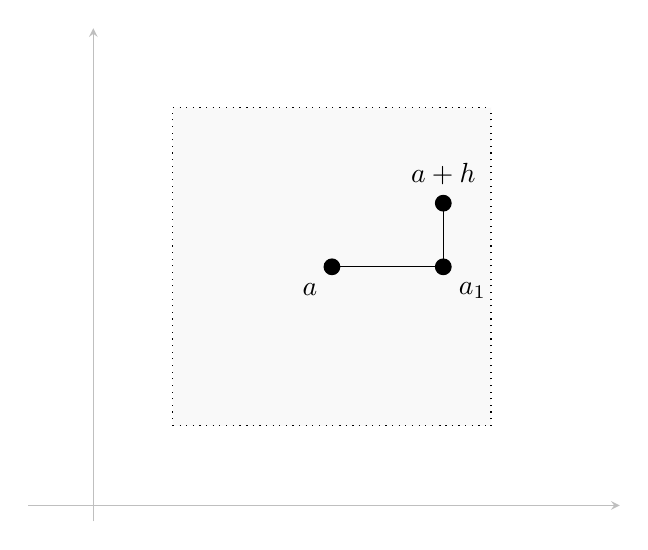
\begin{tikzpicture}
			\begin{axis}[
			xmin=-0.1,xmax=3,
			ymin=-0.1,ymax=3,
			ytick={0},
			xtick={0},
			xticklabels={0},
			yticklabels={0},
			axis lines=middle,
			axis line style=lightgray,
			axis equal,
			width=0.75\textwidth
			]
			\addplot[black,dotted,-] expression[name path=a,domain=0.5:2.5,samples=100]{2.5}; 
			\addplot[black,dotted,-] expression[name path=b,domain=0.5:2.5,samples=100]{0.5}; 
			\addplot[fill=gray, fill opacity=0.05
			]
			fill between[of=a and b,soft clip={domain=0.5:2.5}];
			\addplot +[mark=none,black,dotted] coordinates {(0.5, 0.5) (0.5, 2.5)};
			\addplot +[mark=none,black,dotted] coordinates {(2.5, 0.5) (2.5, 2.5)};
			
			
			\node[label={235:$a$},color=black,draw=black,circle,fill,inner sep=2pt] at (axis cs:1.5,1.5) {}; 
			\node[label={90:$a+h$},color=black,draw=black,circle,fill,inner sep=2pt] at (axis cs:2.2,1.9) {}; 
			\node[label={315:$a_1$},color=black,draw=black,circle,fill,inner sep=2pt] at (axis cs:2.2,1.5) {};
			
			\addplot[black,-] expression[domain=1.5:2.2,samples=2]{1.5};
			\addplot +[mark=none,black,solid] coordinates {(2.2, 1.5) (2.2, 1.9)};
			\end{axis}
			\end{tikzpicture}
		\end{center}
		\caption{A picture of $a, a_1$ and $a_2 = a + h$, as defined in the proof of \cref{continuous-partials}. Defining $\xi_1$ and $\xi_2$ using the mean value theorem as in the proof, the point $a + \xi_1e_1$ is somewhere along the horizontal line joining $a$ and $a+h_1$, and the point $a+h_1 + \xi_2e_2$ is somewhere on the vertical line joining $a+h_1$ and $a+h$.}  \label{continuous-differentiability-picture}
	\end{figure}
	
	Notice that 
	\[ f(a+h) - f(h) = \sum_{i = 1}^m \left( f(a_i) - f(a_{i-1}) \right). \]
	Let us fix $i$ temporarily. Notice that $a_i = a_{i-1} + h_i e_i$, so
	\[ f(a_i) - f(a_{i-1}) = f(a_{i-1}+h_ie_i) - f(a_{i-1}). \]
	Suppose $h_i \neq 0$. We can then apply the mean value theorem \ref{mean-value-theorem}\index{mean value theorem} to the single variable function \[ t \mapsto f(a_{i-1} + te_i) \] on the closed interval between $0$ and $h_i$. This function is well-defined and differentiable on this interval: its derivative at a value $t$ is $\partial_i f(a_{i-1} + te_i)$, by definition of partial derivatives. The mean value theorem \ref{mean-value-theorem}\index{mean value theorem} says that there exists $\xi_i$ between 0 and $h_i$ such that
	\[ \partial_i f(a_{i-1} + \xi_ie_i) = \frac{f(a_{i-1} + h_ie_i) - f(a_{i-1})}{h_i} = \frac{f(a_{i}) - f(a_{i-1})}{h_i}, \]
	or, in other words,
	\[ f(a_i) - f(a_{i-1}) = \xi_i \partial_i f(a_{i-1} + \xi_i e_i). \]
	If $h_i = 0$, we set $\xi_i = 0$ as well. 
	See \cref{continuous-differentiability-picture} again. Unfixing $i$, we find that
	\[ f(a+h) - f(a) = \sum_{i = 1}^m (f(a_i) - f(a_{i-1})) = \sum_{i = 1}^m \xi_i \partial_i f(a_{i-1} + \xi_i e_i). \]
	Thus
	\[ |f(a+h) - f(a)-\ell(h)| \leq \sum_{i = 1}^m |\xi_i| \cdot |\partial_i(a_{i-1}+\xi_ie_i) - \partial_if(a)|. \]
	Since $\partial_if$ is continuous at $a$, there exists $\delta_i > 0$ such that $|\partial_i(a+k) - \partial_i(a)| < \epsilon/m$ for all $|k| < \delta_i$. Let $\delta = \min\{\delta_0, \delta_1, \dotsc, \delta_m\}$. If $|h| < \delta$, then 
	\[ |\partial_i(a_{i-1} + \xi_ie_i) - \partial_i f(a)| < \epsilon/m, \]
	which means that
	\[ |f(a+h) - f(a)-\ell(h)| \leq \sum_{i = 1}^m \frac{|\xi_i| \epsilon}{m} = \frac{\epsilon}{m} \sum_{i = 1}^m |\xi_i| \leq |h| \epsilon , \]
	where we use the fact that $|\xi_i| \leq |h_i|$ for all $i$ for the final step. 
\end{proof}

\begin{unimportantremark}
	If you're using the euclidean norm, you'll have to apply \cref{max-euclidean} for the final step of the proof above. This is another example of why the max norm is often easier to deal with. 
\end{unimportantremark}

Here is another fact that can be proved using a similar argument involving zigzag paths where each segment is orthogonal to the coordinate axes. 

\begin{exercise}
	Suppose $U$ is a convex open subset of $\R^m$ and $f : \R^m \to \R$ is a (not necessarily differentiable) function for which there exists a constant $M > 0$ such that $|\partial_i f(x)| \leq M$ for all $i = 1, \dotsc, m$ and $x \in U$. Prove that $f$ is continuous. 
\end{exercise}

\subsubsection*{Continuous differentiability}

\begin{definition}[Continuously differentiable functions] \index{continuously differentiable} \label{continuously-differentiable-definition}
	We say that $f$ is \emph{continuously differentiable} if $\partial_i f_j : U \to \R$ is continuous for all $i = 1, \dotsc, m$ and $j = 1, \dotsc, n$. \Cref{continuous-partials} guarantees that such a function is, in particular, differentiable. 
\end{definition}

As we saw in the single variable case, continuously differentiable functions have lots of nice properties. For example, recall the calculation we did in \cref{polar-map} showing that the critical locus was a line inside $\R^2$, which is a closed subset. This fact is a special case of the following.

\begin{exercise} \label{critical-locus-closed}
	Suppose $f : U \to \R^n$ is continuously differentiable. Show that the ``critical locus'' of $f$ (ie, the set of all critical points of $f$) is a closed subset of $U$.
\end{exercise}

Here is a multivariable version of the differentiable-but-not-continuously-differentiable function from \cref{power-times-sine}. 

\begin{exercise}
	Let $f : \R^2 \to \R$ denote the following function.
	\[ f(x, y) = \begin{cases} x^2\sin(1/x) + y^2\sin(1/y) & \text{if } x, y \neq 0 \\
	x^2\sin(1/x) & \text{if } x \neq 0 \text{ and } y = 0 \\
	y^2\sin(1/y) & \text{if } x = 0 \text{ and } y \neq 0 \\
	0 & \text{if } x = y = 0 \end{cases} \]
	Show that $f$ is differentiable, but not continuously differentiable. 
\end{exercise}

\begin{exercise} \label{no-continously-differentiable-bijection}
	You might recall proving at some point in a previous class that $\R^2$ and $\R$ have the same cardinality: in other words, that there exists a bijection $f : \R^2 \to \R$. Show that any such bijection cannot be continuously differentiable. 
	
	\begin{hint}
		Suppose for a contradiction that $f : \R^2 \to \R$ is a continuously differentiable bijection.  Let $U$ be an open subset of $\R^2$ such that $\partial_1 f(x, y) \neq 0$ for all $(x,y) \in U$, and then consider the function $g : U \to \R^2$ given by $g(x, y) = (f(x, y), y)$. 
	\end{hint}
\end{exercise}

\begin{proposition} \label{c1-stable-inversion}
	Suppose $f : U \to \R^n$ is continuously differentiable, open, and injective. Then $f^{-1}$ is also continuously differentiable. 
\end{proposition} 

\begin{proof}
	We know from \cref{inverse-differentiable} that $f^{-1}$ is differentiable and that  
	\[ d(f^{-1})_y = (df_{f^{-1}(y)})^{-1} \]
	for all $y \in U$. Taking standard matrix representations, we get
	\[ [d(f^{-1})_y] = [(df_{f^{-1}(y)})^{-1}] = [df_{f^{-1}(y)}]^{-1}.  \]
	By \cref{jacobian-matrix}, the $(j,i)$-entry on the left hand side is $\partial_i (f^{-1})_j(y)$, so this equality says that $\partial_i (f^{-1})_j : f(U) \to \R$ is equal to the following composite. 
	\[ \begin{tikzcd} f(U) \ar{r}{f^{-1}} & U \ar{rr}{x \mapsto [df_x]} & & \GL_n \ar{rr}{A \mapsto A^{-1}} & & \GL_n \ar{rr}{(j,i)-\text{entry}} & & \R \end{tikzcd} \]
	Here $\GL_n$ denotes the set of invertible $n \times n$ matrices as in \cref{matrix-norm}. Each of the functions being composed here is continuous (cf. 
	\cref{differentiable-implies-continuous,matrix-inversion-homeomorphism}), so we conclude that $\partial_i (f^{-1})_j$ is continuous.  
\end{proof}

\subsubsection*{Continuous differentiability and continuity of the derivative \starred}

For this section, we will need to make substantial use of the continuity properties of the operator norm. But it's also not terribly important. The main result of this section, \cref{continuously-differentiable}, is aesthetically rather satisfying, and can occasionally streamline proofs. 

\begin{lemma} \label{continuously-differentiable-by-components}
	Suppose $f : U \to \R^n$ is differentiable. Then $df : U \to \mathscr{L}(\R^m, \R^n)$ is continuous if and only if $df_j : U \to \mathscr{L}(\R^m, \R)$ is continuous for all $j = 1, \dotsc, n$. 
\end{lemma}

\begin{proof}
	We will use \cref{differentiable-by-components}, which tells us that $f$ is differentiable if and only if $f_j$ is differentiable for all $j = 1, \dotsc, n$, and moreover that $df_{j,a} = \pi_j \circ df_a$ for all $a \in U$. In other words, the following diagram commutes. 
	\[ \begin{tikzcd} U \ar{r}{df} \ar[bend right]{dr}[swap]{df_j} & \mathscr{L}(\R^m, \R^n) \ar{d}{\pi_j \circ -} \\ & \mathscr{L}(\R^m, \R) \end{tikzcd} \]
	You will verify in \cref{continuously-differentiable-by-components-exercise} below that the map ``postcompose with $\pi_j$'' map $\pi_j \circ - : \mathscr{L}(\R^m, \R^n) \to \mathscr{L}(\R^m, \R)$ is continuous. Thus, if $df$ is continuous, then $df_j$ is also continuous. 
	
	Conversely, suppose that $df_j$ is continuous for all $j$. Let us show that $df$ is continuous at any $a \in U$. Suppose $\epsilon > 0$. Since $df_j$ is continuous at $a$, there exists $\delta_j > 0$ such that \[ \|df_{j,x} - df_{j,a}\| < \frac{\epsilon}{\sqrt{n}} \] for all $x \in U$ such that $|x - a| < \delta_j$. Let $\delta := \min\{\delta_1, \dotsc, \delta_n\}$. Then $\|df_x - df_a\| < \epsilon$ for all $x \in U$ such that $|x-a| < \delta$, as you will verify in \cref{continuously-differentiable-by-components-exercise} below. 
\end{proof}

\begin{exercise} \label{continuously-differentiable-by-components-exercise}
	\begin{enumerate}[(a)]
		\item Check that the ``postcompose with $\pi_j$'' map $\mathscr{L}(\R^m, \R^n) \to \mathscr{L}(\R^m, \R)$ (ie, the one  given by $\phi \mapsto \pi_j \circ \phi$) is continuous. Alternatively, prove the more general statement given in \cref{composition-continuous} and then derive this statement.   
		\item With notation as in the latter part of the proof above, verify that $\|df_a - df_b\| < \epsilon$. 
	\end{enumerate}
\end{exercise}

\begin{proposition} \label{continuously-differentiable}
	Suppose $f : U \to \R^n$ is differentiable. Then $f$ is continuously differentiable if and only if $df : U \to \mathscr{L}(\R^m, \R^n)$ is continuous. 
\end{proposition}

\begin{proof}
	Thanks to \cref{continuously-differentiable-by-components}, we can assume without loss of generality that $n = 1$. If $f$ is differentiable, then \cref{differentiable-implies-directionals} tells us that $\partial_i f = df(e_i)$. In other words, the following diagram commutes.
	\[ \begin{tikzcd} U \ar{r}{df} \ar[bend right]{dr}[swap]{\partial_i f} & \mathscr{L}(\R^m, \R) \ar{d}{\text{``evaluate at $e_i$''}} \\ & \R \end{tikzcd} \]
	The ``evaluate at $e_i$'' map is continuous by \cref{evaluation-continuous}. So, if $df$ is continuous, then $\partial_i f$ must also be continuous, as it is the composite of two continuous functions. The converse is left as an exercise; see \cref{continuously-differentiable-details} below. 
\end{proof}

\begin{exercise} \label{continuously-differentiable-details}
	\begin{enumerate}[(a)]
		\item Elaborate on the first sentence of the above proof (in other words, explain why proving \cref{continuous-partials} for $n = 1$ is sufficient to prove it for all $n$). 
		\item If you haven't already done it, do \cref{evaluation-continuous}. 
		\item Complete the proof above by showing that $df : U \to \mathscr{L}(\R^m, \R)$ is continuous if $f$ is continuously differentiable. 
	\end{enumerate}
\end{exercise}

\begin{remark}
	This reformulation of continuous differentiability is often convenient in proofs. For example, in the proof of \cref{c1-stable-inversion}, we calculated that
	\[ d(f^{-1})_y = (df_{f^{-1}(y)})^{-1}. \]
	This says that the $d(f^{-1}) = \text{inversion} \circ df \circ f^{-1}$. 
	\[ \begin{tikzcd} f(U) \ar{d}[swap]{f^{-1}} \ar{r}{d(f^{-1})} & \GL(\R^n) \\ U \ar{r}{df} & \GL(\R^n) \ar{u}[swap]{\text{inversion}}  \end{tikzcd} \]
	We know that $f^{-1}$ is continuous; $df$ is continuous by \cref{continuously-differentiable}, and inversion is continuous by \cref{linear-map-inversion-homeomorphism}. Thus $d(f^{-1})$ is continuous, so \cref{continuously-differentiable} implies that $f^{-1}$ is continuously differentiable. 
\end{remark}

\subsection{\texorpdfstring{$C^k$}{Ck} functions}

\begin{definition}[$C^k$ functions] \label{ck} \index{ck@$C^k$}
	We say that a function $f : U \to \R^n$ is $C^0$ if it is continuous. Then, inductively, for any positive integer $k$, we say that a function $f : U \to \R^n$ is $C^k$ if the partial derivatives $\partial_i f_j$ all exist and are $C^{k-1}$ functions $U \to \R$. 
\end{definition}

By definition, $f : U \to \R^n$ is $C^1$ if and only if it is continuously differentiable. It is clear from the definitions that a function $f : U \to \R^n$ is $C^k$ if and only if its component functions $f_j : U \to \R$ are $C^k$. Here are some results showing that reasonable ways of combining $C^k$ functions still yield $C^k$ functions. 

\begin{exercise} \label{ck-stable-sum-scalar}
	Show that the set of all $C^k$ functions $U \to \R^n$ form a vector space. 
\end{exercise} 

\begin{exercise} \label{ck-stable-composite}
	Suppose $U$ is an open subset $\R^m$, that $V$ is an open subset of $\R^n$, and that $f : U \to \R^n$ and $g : V \to \R^p$ are both $C^k$, and that $f(U) \subseteq V$. Show that $g \circ f$ is also $C^k$. 
\end{exercise}

\begin{exercise} \label{ck-stable-product}
	Suppose $f, g : U \to \R$ are both $C^k$. Show that $fg$ is also $C^k$. 
\end{exercise}

\begin{exercise} \label{ck-stable-reciprocal}
	Suppose $f : U \to \R$ is $C^k$ and $f(x) \neq 0$ for all $x \in U$. Show that $1/f$ is also $C^k$.
	\begin{hint}
		Note that $1/f$ is $f$ composed with the single variable inversion function. 
	\end{hint}
\end{exercise}

\begin{exercise} \label{ck-stable-inversion}
	Suppose $f : U \to \R^n$ is \'etale, injective, and $C^k$ for some $k \geq 1$. Show that $f^{-1}$ is also $C^k$. 
	\begin{hint}
		This is a multivariable version of \cref{ck-stable-inversion-single}, and can be proved by using a similar induction. Some ingredients you might think about combining are the inverse function theorem \ref{inverse-function-theorem} and  \cref{c1-stable-inversion,matrix-inversion-homeomorphism} (and their proofs). 
	\end{hint}
\end{exercise}

\subsection{Equality of mixed partials \starred}

\begin{definition}[Mixed partials] \index{mixed partials}
	Suppose $f : U \to \R$ is $C^2$. The partial derivative $\partial_i f : U \to \R$ for any $i = 1, \dotsc, m$ is a continuously differentiable function, so its $j$th partial deriative $\partial_j( \partial_i f)$ is a continuous function $U \to \R$ for any $j = 1, \dotsc m$. We denote the function $\partial_j(\partial_i f)$ more succinctly as $\partial_{j,i} f$, or as
	\[ \frac{\partial^2 f}{\partial x_j \partial x_i} \]
\end{definition}

\begin{theorem}[Equality of mixed partials] \label{mixed-partials} \index{mixed partials!equality of mixed partials}
	Suppose $f : U \to \R$ is $C^2$. Then, for all $i, j = 1, \dotsc, m$, we have $\partial_{j,i} f = \partial_{i,j} f$.
\end{theorem}

\begin{proof}
	Observe that
	\[ \begin{aligned} \partial_{j,i} f(a) &= \lim_{t_j \to 0} \frac{\partial_i f(a + t_j e_j) - \partial_i f(a)}{t_j} \\
	&= \lim_{t_j \to 0} \frac{ \displaystyle \lim_{t_i \to 0} \frac{f(a + h_i e_i + t_j e_j) - f(a + t_j e_j)}{t_i} - \lim_{t_i \to  0} \frac{f(a + t_i e_i) - f(a)}{t_i} }{t_j} \\
	&= \lim_{t_j \to 0} \lim_{t_i \to 0} \frac{f(a + t_i e_i + t_j e_j) - f(a+t_i e_i) - f(a + t_j e_j) + f(a)}{t_i t_j}. \end{aligned} \]
	Notice that, if we unwind the definition of $\partial_{i,j} f(a)$ in the same way, we end up taking a double limit of the same expression, but the order of the limits is interchanged. In other words, if we define
	\[ \sigma(t_i, t_j) = \frac{f(a + t_i e_i + t_j e_j) - f(a+t_i e_i) - f(a + t_j e_j) + f(a)}{t_i t_j},  \]
	then
	\[ \partial_{j,i} f(a) = \lim_{t_j \to 0} \lim_{t_i \to 0} \sigma(t_i, t_j) \quad \text{ whereas } \quad \partial_{i,j}f(a) = \lim_{t_i \to 0} \lim_{t_j \to 0} \sigma(t_i, t_j). \]
	So, to prove the theorem, it is sufficient to prove that
	\[ \partial_{j,i} f(a) = \lim_{t \to 0} \sigma(t,t). \]
	
	Fix a nonzero real number $t$ and consider the function
	\[ \alpha(s) = f(a + se_i + te_j) - f(a + se_i). \]
	Notice that
	\[ \sigma(t,t) = \frac{\alpha(t)-\alpha(0)}{t^2} \]
	and that $\alpha$ is differentiable with \[ \alpha'(s) = \partial_i f(a + se_i + te_j) - \partial_i f(a + se_i). \]
	Applying the mean value theorem \ref{mean-value-theorem}\index{mean value theorem} to $\alpha$ on the closed interval between 0 and $t$, there exists $\xi_i(t)$, strictly between 0 and $t$, such that
	\[ \sigma(t,t) = \frac{\alpha(t) - \alpha(0)}{t^2} = \frac{\alpha'(\xi_i(t))}{t} = \frac{\partial_i f(a + \xi_i(t) e_i + te_j) - \partial_i f(a + \xi_i(t) e_i)}{t}. \]
	Now consider the function 
	\[ \beta(s) = \partial_i f(a + \xi_i(t) e_i + se_j). \]
	Then $\beta$ is differentiable with
	\[ \beta'(s) = \partial_{j,i} f(a + \xi_i(t) e_i + se_j), \]
	so, applying the mean value theorem \ref{mean-value-theorem}\index{mean value theorem} to $\beta$ on the closed interval between 0 and $t$, we find that there exists $\xi_j(t)$, strictly between 0 and $t$, such that
	\[ \sigma(t,t) = \frac{\beta(t) - \beta(0)}{t} = \beta'(\xi_j(t)) = \partial_{j,i} f(a + \xi_i(t) e_i + \xi_j(t) e_j). \]
	Now notice that, since both $\xi_i(t)$ and $\xi_j(t)$ are between 0 and $h$, we have $\xi_i(t), \xi_j(t) \to 0$ as $t \to 0$. Since $\partial_{j,i} f$ is continuous at $a$, we have
	\[ \lim_{t \to 0} \sigma(t,t) = \lim_{t \to 0} \partial_{j,i} f (a + \xi_i(t)e_i + \xi_j(t)e_j) = \partial_{j,i} f(a). \qedhere \]
\end{proof}

\begin{remark}
	If $f : U \to \R$ is $C^2$, the \emph{hessian} of $f$ at $a$, denoted $f''(a)$,\index{hessian} is the matrix of second partial derivatives. 
	\[ f''(a) = \begin{bmatrix} \partial_{1,1} f(a) & \partial_{1,2} f(a) & \dotsb & \partial_{1,m} f(a) \\
	\vdots & \vdots & \ddots & \vdots \\
	\partial_{m,1} f(a) & \partial_{m,2} f(a) & \dotsb & \partial_{m,m} f(a) \end{bmatrix} \]
	\Cref{mixed-partials} is equivalent to the assertion that $f''(a)$ is a symmetric matrix. 
\end{remark}

There are many versions of this theorem, all with slightly different hypotheses. For instance, there is the version due to Peano \cite[theorem 9.41]{rudin}. In any case, it's worth remarking that some continuity condition on the mixed partials is crucial; it is not enough that the mixed partials exist.

\begin{exercise}
	Consider the following function $f : \R^2 \to \R$. 
	\[ f(x,y) = \begin{cases} xy \dfrac{x^2 - y^2}{x^2 + y^2} & \text{if } (x,y) \neq 0 \\ 0 &  \text{if } (x,y) = 0 \end{cases} \]
	\begin{enumerate}[(a)]
		\item Calculate all of the following. 
		\[ \frac{\partial f}{\partial x} \quad \frac{\partial f}{\partial y} \quad \frac{\partial^2 f}{\partial y \partial x} \quad \frac{\partial^2 f}{\partial x \partial y} \]
		\item Show that the mixed partials are discontinuous at the origin. 
		\item Show that the mixed partials disagree at the origin. 
	\end{enumerate}
\end{exercise}

\subsection{Taylor's theorem \starred} 

The main difficulty in the multivariable Taylor's theorem is notation; we've already done most of the hard work of the proof with the single variable version (cf.  \cref{taylor-single,taylor-single-remainder-lagrange}). Let us first discuss some typical notation conventions that make the statement of Taylor's theorem more readable. 

\subsubsection*{Multi-index notation}

\begin{definition}[Multi-index notation] \index{multi-index} \label{multi-index}
	A \emph{multi-index} is an $m$-tuple $\alpha = (\alpha_1, \dotsc, \alpha_m)$ where $\alpha_i$ is a non-negative integer. For a multi-index $\alpha$ and any non-negative integer $\ell$, we define the following. 
	\[ \begin{aligned} |\alpha| &= \alpha_1 + \alpha_2 + \dotsb + \alpha_n \\ \alpha! &= \alpha_1! \alpha_2! \dotsb \alpha_m ! \\
	\binom{\ell}{\alpha} &= \frac{\ell!}{\alpha!} = \frac{\ell!}{\alpha_1! \dotsb \alpha_m!} \end{aligned} \]
	If $\alpha$ and $\beta$ are both multi-indices, we define the sum $\alpha + \beta$ componentwise; then we have $|\alpha + \beta| = |\alpha| + |\beta|$. We let $0$ denote the multi-index $(0, 0, \dotsc, 0)$, and for each $i = 1, \dotsc, m$, we let $1_i$ denote the multi-index that is 1 in position $i$ and zero everywhere else.
	
	If $x = (x_1, \dotsc, x_m) \in \R^m$, we define
	\[ x^\alpha = x_1^{\alpha_1} x_2^{\alpha_2} \dotsb x_m^{\alpha_m}. \]
	In particular, we have $x^0 = 1$ and $x^{1_i} = x_i$. 
	Also, if $f : U \to \R$ is $C^{|\alpha|}$, we define
	\[ \partial^\alpha f = \partial_1^{\alpha_1} \partial_2^{\alpha_2} \dotsb \partial_m^{\alpha_m} f, \]
	where we use the convention that $\partial^{0} f = f$. In particular, we have $\partial^{1_i} f = \partial_i f$. 
\end{definition}

\begin{caution}
	Note that, the way we've set up notation, superscripts and subscripts on $\partial$ denote distinct concepts. For example, if $f : \R^2 \to \R$ is a function, $\partial_{(1,1)}f(a)$ denotes the directional derivative in the direction of the vector $(1,1)$, while $\partial^{(1,1)}f(a)$ is the mixed partial derivative $\partial_{1,2}f(a)$. 
\end{caution}

We now establish some rules for doing algebra with multi-indices. 

\begin{exercise}
	Suppose $\alpha, \beta$ are multi-indices and $x = (x_1, \dotsc, x_m) \in \R^m$. Prove that \[ x^\alpha x^\beta = x^{\alpha + \beta}. \]
\end{exercise}

\begin{exercise}[Equality of mixed partials, multi-index version] \label{mixed-partials-multi-index}
	Suppose $\alpha, \beta$ are multi-indices and $f : U \to \R$ is $C^{|\alpha + \beta|}$. Prove that \[ \partial^\alpha \partial^\beta f = \partial^{\alpha + \beta} f. \] 
	\begin{hint}
		First consider the case when $\alpha = 1_i$ for some $i = 1, \dotsc, m$. Prove this by induction on $|\beta|$. 
	\end{hint}
\end{exercise}

There is a convenient combinatorial interpretation of $\binom{\ell}{\alpha}$ when $\ell = |\alpha|$ which generalizes the combinatorial interpretation of binomial coefficients. For this reason, the $\binom{\ell}{\alpha}$ are often called ``multinomial coefficients.''\index{multinomial}

\begin{theorem} \label{multinomial-combinatorial}
	Suppose $\alpha$ is a multi-index and $\ell = |\alpha|$. Then the multinomial coefficient $\binom{\ell}{\alpha}$ is the number of ways of placing $\ell$ objects into $m$ bins, with $\alpha_1$ objects in the first bin, $\alpha_2$ objects in the second bin, and so on. In particular, $\binom{\ell}{\alpha}$ is a positive integer. 
\end{theorem}

\begin{proof}
	The number of ways of choosing $\alpha_1$ objects out of the $\ell$ to place in the first bin is
	\[ \binom{\ell}{\alpha_1}. \]
	Now we have $\ell - \alpha_1$ objects remaining, and the number of ways of choosing $\alpha_2$ of them to be placed into the second bin is 
	\[ \binom{\ell - \alpha_1}{\alpha_2}. \]
	Continuing in this way, the total number of ways of placing the $\ell$ objects into the first $m$ bins is the product of all of these binomial coefficients
	\[ \binom{\ell}{\alpha_1} \binom{\ell - \alpha_1}{\alpha_2} \dotsb \binom{\ell - \alpha_1 - \dotsb - \alpha_{m-1}}{\alpha_m}. \]
	But if we expand out each of these binomial coefficients, this product is 
	\[ \frac{\ell!}{\alpha_1!(\ell - \alpha_1)!} \frac{(\ell - \alpha_1)!}{\alpha_2!(\ell - \alpha_1 - \alpha_2)!} \dotsb \frac{(\ell - \alpha_1 - \dotsb - \alpha_{m-1})!}{\alpha_m!(\ell - \alpha_1 - \dotsb - \alpha_m)!} = \binom{\ell}{\alpha} \]
	because the numerator in each of the fractions starting from the second cancels with one of the terms in the denominator of the previous fraction, and because $|\alpha| = \ell$ means that $(\ell - \alpha_1 - \dotsb - \alpha_m)! = 1$. 
\end{proof}

\begin{corollary} \label{multinomial-recurrence}
	Suppose $\alpha'$ is a multi-index and $|\alpha'| = \ell + 1$. Then
	\[ \binom{\ell + 1}{\alpha'} = \sum_{\alpha' = \alpha + 1_i} \binom{\ell}{\alpha}, \]
	where the sum is over all $\alpha$ such that $\alpha' = \alpha + 1_i$ for some $i$. 
\end{corollary}

\begin{proof}
	Suppose we want to place $\ell + 1$ objects into $m$ bins with $\alpha'_i$ objects in the $i$th bin for all $i$. On the one hand, \cref{multinomial-combinatorial} tells us that the left hand side is the number of ways of doing this. On the other hand, if $\alpha_i' \geq 1$, then there is a unique multi-index $\alpha$ such that $\alpha' = \alpha + 1_i$. We can place the first object in bin $i$, then the number of ways of distributing the remaining $\ell$ objects is $\binom{\ell}{\alpha}$. Summing over all such $i$ yields precisely the sum on the right hand side. 
\end{proof}

\begin{exercise}[Multinomial theorem] \label{multinomial}
	Prove that, for any $x = (x_1, \dotsc, x_m) \in \R^m$, we have 
	\[ (x_1 + \dotsb + x_m)^\ell = \sum_{|\alpha| = \ell} \binom{\ell}{\alpha} x^\alpha. \]
	\begin{hint}
		You can do it by induction. A more insightful proof involves using the combinatorial interpretation of  \cref{multinomial-combinatorial}. 
	\end{hint} 
\end{exercise}

Multi-index notation also gives us compact notation for multivariable polynomials. 

\begin{definition}
	A \emph{polynomial} $p$ in $m$ variables is a function $\R^m \to \R$ of the form
	\[ p(x) = \sum_\alpha c_\alpha x^\alpha \]
	where $x = (x_1, \dotsc, x_m) \in \R^m$, the sum is over all multi-indices, and for every multi-index $\alpha$, we have $c_\alpha \in \R$ and $c_\alpha = 0$ for all but finitely many $\alpha$ (ie, the sum displayed above is finite). The \emph{degree} of $p$ is the maximum $|\alpha|$ such that $c_\alpha \neq 0$. If $p = 0$, we define its degree to be $-\infty$. 
\end{definition}

\begin{exercise} \label{small-polynomial-is-zero}
	Suppose $p$ is a polynomial of degree at most $k$ in $m$ variables. If $|p(h)| = o(|h|^k)$ as $h \to 0$, show that $p = 0$. 
\end{exercise}

\subsubsection*{Statement of Taylor's theorem}

We're now ready to state the multivariable version of Taylor's theorem. 

\begin{theorem}[Taylor] \label{taylor}
	Suppose $U$ is a convex open set, $f : U \to \R$ is $C^k$ for some non-negative integer $k$, and $a \in U$. Then there exists a unique polynomial $p_k$ of degree at most $k$ in $m$ variables, called the \emph{degree $k$ Taylor polynomial of $f$ at $a$}, such that $|f(a+h) - p_k(h)| = o(|h|^k)$ as $h \to 0$. Moreover, we have
	\begin{equation} \label{taylor-polynomial} p_k(h) = \sum_{|\alpha| \leq k} \frac{\partial^\alpha f(a)}{\alpha!} h^\alpha. \end{equation}
	Finally, if $f$ is $C^{k+1}$, then for any $h$ such that $a + h \in U$, there exists $\xi$ on the line segment between $a$ and $a+h$ such that 
	\[ f(a+h) - p_k(h) = \sum_{|\alpha| = k+1} \frac{\partial^\alpha f(\xi)}{\alpha!} h^{k+1}. \]
\end{theorem}

While the notation for the Taylor polynomial is compact and aesthetically pleasing, there's a lot of information packed into very few symbols. Here is an example. 

\begin{example} \label{taylor-example}
	Let $U = \R^2 \setminus \{0\}$ and let $f : U \to \R^2$ be the function \[ f(x,y) = \ln(x^2 + y^2). \]
	See \cref{taylor-example-graph}
	\begin{figure}[ht]
		\begin{center}
			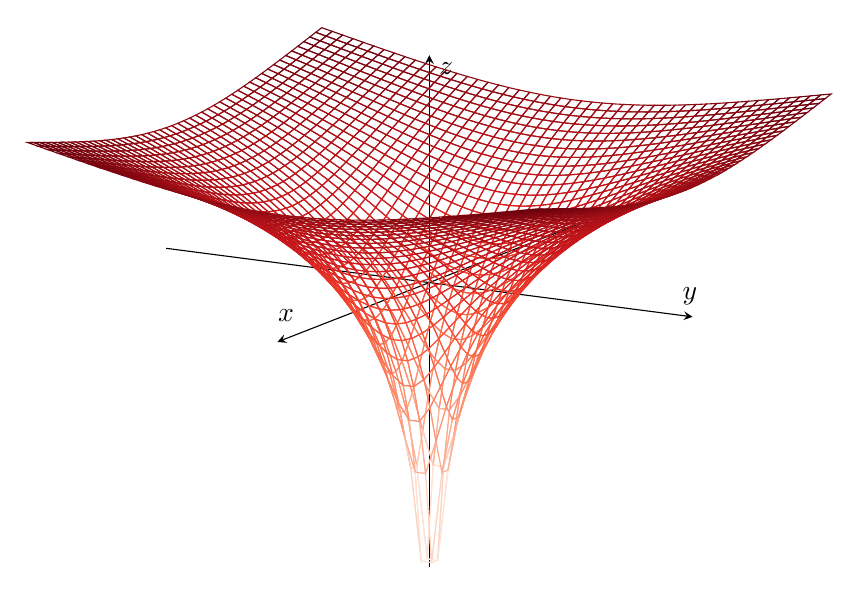
\begin{tikzpicture}
			\begin{axis}[
			view={120}{15},
			axis lines=middle,
			xlabel={$x$},
			xtick={0},
			xmin=-3.1,xmax=3.1,
			ylabel={$y$},
			ytick={0},
			ymin=-3.1,ymax=3.1,
			zlabel={$z$},
			ztick={0},
			zmin=-5,zmax=4,
			width=\textwidth,
			]
			\addplot3[mesh,samples=50,domain=-3:3,colormap/Reds]{ln(x^2+y^2)}; 
			\end{axis}
			\end{tikzpicture}
		\end{center}
		\caption{The graph of the function  $f(x,y) = \ln(x^2 + y^2)$. } \label{taylor-example-graph}
	\end{figure}
	
	Let's calculate the degree 2 Taylor polynomial of $f$ at the point $(1,0)$. First of all, we have \[ f(1,0) = 0, \] which tells us the constant term of the polynomial. The linear terms in the Taylor polynomial will depend on the partial derivatives of $f$. More precisely, note that there are two multi-indices $\alpha$ with $|\alpha| = 1$, which are $\alpha = (1,0)$ and $\alpha = (0,1)$. We have the following.  
	\[ \begin{aligned} \partial^{(1,0)}f(1,0) &= \frac{\partial f}{\partial x}(1,0) = \left.\frac{2x}{x^2 + y^2}\right|_{(x,y) = (1,0)} = 2 \\
	 \partial^{(0,1)}f(1,0) &= \frac{\partial f}{\partial y}(1,0) = \left.\frac{2y}{x^2 + y^2}\right|_{(x,y) = (1,0)} = 0 \end{aligned} \]
	The quadratic terms of the polynomial will depend on the second order partial derivatives, ie, on $\partial^\alpha f(1,0)$ where $|\alpha| = 2$. There are three such multi-indices: $(2,0), (1,1)$, and $(0,2)$. We have the following. 
	\[ \begin{aligned} \partial^{(2,0)}f(1,0) &= \left.\frac{\partial^2 f}{\partial x^2}(1,0) = \frac{2y^2 - 2x^2}{(x^2 + y^2)^2}\right|_{(x,y) = (1,0)} = -2 \\
	\partial^{(1,1)}f(1,0) &= \frac{\partial^2 f}{\partial y \partial x}(1,0) = \left.\frac{-4xy}{(x^2 + y^2)^2}\right|_{(x,y) = (1,0)} = 0 \\
	\partial^{(0,2)}f(1,0) &= \frac{\partial^2 f}{\partial y^2}(1,0) = \left.\frac{2x^2 - 2y^2}{(x^2 + y^2)^2}\right|_{(x,y) = (1,0)} = 2 \end{aligned} \]
	You may find it convenient to organize your partial derivative calculations in a tree-like diagram, as in \cref{partial-derivatives-tree}. 
	\begin{figure}
		\begin{center}
			\begin{tikzpicture}
			\node (A) at (0,0) {$\ln(x^2+y^2)$};
			
			\node (B) at (-3,-3) {$\dfrac{2x}{x^2+y^2}$};
			\node (C) at (3,-3) {$\dfrac{2y}{x^2+y^2}$};
			
			\node (D) at (-6,-6) {$\dfrac{2y^2-2x^2}{(x^2+y^2)^2}$};
			\node (E) at (0,-6) {$\dfrac{-4xy}{(x^2+y^2)^2}$};
			\node (F) at (6,-6) {$\dfrac{2x^2-2y^2}{(x^2+y^2)^2}$};
			
			
			\begin{scope}[every node/.style={fill=white,circle}]
			\path [->] (A) edge node {$\partial_x$} (B);
			\path [->] (A) edge node {$\partial_y$} (C);
			
			\path [->] (B) edge node {$\partial_x$} (D);
			\path [->] (B) edge node {$\partial_y$} (E);
			\path [->] (C) edge node {$\partial_x$} (E);
			\path [->] (C) edge node {$\partial_y$} (F);
			\end{scope}
			\end{tikzpicture}
		\end{center}
		\caption{Iterated partial derivatives of the function $f(x,y) = \ln(x^2+y^2)$.} \label{partial-derivatives-tree}
	\end{figure}
	
	These calculations let us assemble the degree 2 Taylor polynomial. 
	\[ \begin{aligned} p_2(h,k) &= f(1,0) (h,k)^{(0,0)} + \frac{\partial^{(1,0)}f(1,0)}{(1,0)!}(h,k)^{(1,0)} + \frac{\partial^{(0,1)}f(0,1)}{(0,1)!}(h,k)^{(0,1)}  \\
	&\quad + \frac{\partial^{(2,0)}f(1,0)}{(2,0)!}(h,k)^{(2,0)} + \frac{\partial^{(1,1)}f(1,0)}{(1,1)!}(h,k)^{(1,1)} + \frac{\partial^{(0,2)}f(1,0)}{(0,2)!}(h,k)^{(0,2)} \\
	&= 2h - h^2 + k^2. \end{aligned} \]
	Taylor's theorem \ref{taylor} states roughly that $f(1+h,k) \approx 2h - h^2 + k^2$ for small $(h,k)$. More precisely, the assertion is that the difference between the left and right hand sides above is $o(|(h,k)|^2)$ as $(h,k) \to 0$. 
\end{example}

I exhort you to work through the following example yourself before proceeding. It may start feeling tedious at some point, but power through it. Facility with calculating explicit examples is what gives you the intuition you need to do abstract proofs. 

\begin{exercise}
	Let $f : \R^2 \to \R$ be the function $f(x,y) = \sin(xy^2)$. Calculate the degree 3 Taylor polynomial of $f$ at the origin. 
\end{exercise}

Here is some practice using the statement of Taylor's theorem in proofs. 

\begin{exercise}
	Let $f : \R^2 \to \R$ be a $C^2$ function. Suppose $a \in \R^2$ is a critical point of $f$ and $\partial^{(1,1)}f(a) = 0$. Use the degree 2 Taylor polynomial of $f$ at $a$ to formulate a rule for determining whether or not $a$ is a local extremum, and if it is, what kind of a local extremum it is. Then prove your rule. 
\end{exercise}

\subsubsection*{Proof of Taylor's theorem}

\begin{proof}[Proof of Taylor's theorem \ref{taylor}]
	We begin with a calculation. Fix $h = (h_1, \dotsc, h_m) \in \R^m$ such that $a + h \in B$ and consider the function $\gamma(t) = a + th$. Note that $\gamma'(t) = h$, and all higher derivatives of $\gamma$ vanish. Then $g = f \circ \gamma$ is a single variable $C^k$ function, and we claim that 
	\begin{equation} \label{iterated-derivative-restricted-to-line} g^{(\ell)}(t) = \sum_{|\alpha| = \ell} \binom{\ell}{\alpha} (\partial^\alpha f \circ \gamma)(t) h^\alpha \end{equation}
	for all $t \in [0,1]$ and $\ell = 0, 1, \dotsc, k$. When $\ell = 0$, \cref{iterated-derivative-restricted-to-line} is just the definition of $g$. We'll actually prove \cref{iterated-derivative-restricted-to-line} in general by induction on $\ell$, and $\ell = 0$ suffices for the base case for this induction; that said, because the notation gets a bit dense, it is instructive to look at a couple of small values of $\ell$ separately to help us understand the general inductive step. 
	
	The case when $\ell = 1$ follows quickly from the chain rule. Indeed, we have $\gamma'(t) = h$, so
	\[ g'(t) = f'(\gamma(t))\gamma'(t) = \sum_{i = 1}^m \partial_i f(\gamma(t))h_i, \]
	using \cref{jacobian-matrix} for the second step. This is precisely equivalent to \cref{iterated-derivative-restricted-to-line} for $\ell = 1$. 
	
	Now consider the case when $\ell = 2$. For any $i = 1, \dotsc, m$, we can calculate the derivative of $\partial_i f \circ \gamma$ using the chain rule. We have
	\[ \begin{aligned} (\partial_i f \circ \gamma)'(t) &= (\partial_i f)'(\gamma(t))\gamma'(t) \\
	&= \sum_{j = 1}^m \partial_{j,i} f (\gamma(t)) h_j \end{aligned} \]
	which means that 
	\[ \begin{aligned} g''(t) &= \sum_{i = 1}^n \sum_{j = 1}^m \partial_{j,i} f(\gamma(t)) h_j h_i \\
	&= \sum_{j < i} 2\partial_{j,i}f(\gamma(t)) h_j h_i + \sum_i \partial_{i,i} f(\gamma(t)) h_i^2 \end{aligned} \]
	where we have used the equality of mixed partials \ref{mixed-partials} for the second step. This too is equivalent to \cref{iterated-derivative-restricted-to-line}, because a multi-index $\alpha$ such that $|\alpha| = 2$ either is 2 in one entry and 0 everywhere else (in which case $\alpha! = 2$ so $\binom{2}{\alpha} = 1$), or else is 1 in two entries and 0 everywhere else (in which case $\alpha! = 1$ so $\binom{2}{\alpha} = 2$).
	
	Now for the general inductive step. Suppose we know \cref{iterated-derivative-restricted-to-line} for some non-negative integer $\ell$. The chain rule then gives us the second step in the following. 
	\[ \begin{aligned} g^{(\ell+1)}(t) &= \frac{d}{dt} \sum_{|\alpha| = \ell} \binom{\ell}{\alpha} (\partial^\alpha \circ \gamma)(t) h^\alpha \\
	&= \sum_{|\alpha| = \ell} \binom{\ell}{\alpha} \left( (\partial^\alpha f)'(\gamma(t)) h \right) h^\alpha \\
	&= \sum_{|\alpha| = \ell} \sum_{i = 1}^m \binom{\ell}{\alpha} \partial^{\alpha + 1_i} f(\gamma(t)) h^{\alpha + 1_i} \\
	&= \sum_{|\alpha| = \ell} \sum_{i = 1}^m \binom{\ell}{\alpha} (\partial^{\alpha + 1_i} f \circ \gamma)(t) h^{\alpha + 1_i} \\
	&= \sum_{|\alpha'| = \ell + 1} \binom{\ell + 1}{\alpha'} (\partial^{\alpha'}f \circ \gamma)(t) h^{\alpha'}  \end{aligned} \]
	We have used \cref{jacobian-matrix} together with equality of mixed partials (in the multi-index form of \cref{mixed-partials-multi-index}) for the third equality, and \cref{multinomial-recurrence} for the final equality. This completes the induction and proves \cref{iterated-derivative-restricted-to-line}. 
	
	We'll prove the ``with remainder'' form of \cref{taylor} first, and then use it to prove the ``without remainder'' form, as in \cite[section 2.4]{konigsberger}. Suppose $f$ is $C^{k+1}$. Then the single variable function $g$ defined above is also $C^{k+1}$. The single variable version of Taylor's theorem with remainder \ref{taylor-single} tells us that
	\[ g(1) = \sum_{\ell = 0}^k \frac{g^{(\ell)}(0)}{\ell!} + \frac{g^{(k+1)}(s)}{(k+1)!} \]
	for some $s \in (0,1)$. But then, applying \cref{iterated-derivative-restricted-to-line}, this equation says precisely that 
	\[ f(a+h) = p_k(h) + \sum_{|\alpha| = k+1} \frac{\partial^{\alpha} f(\xi)}{\alpha!} h^\alpha \]
	for $\xi = a + sh$, where $p_k$ is the polynomial defined in \cref{taylor-polynomial}. 
	
	Now let us prove the existence part of the ``without remainder'' form. In other words, we want to prove that, if $f$ is $C^k$ and $p_k$ is defined as in \cref{taylor-polynomial}, then $|f(a+h) - p_k(h)| = o(|h|^k)$ as $h \to 0$. If $k = 0$, this follows immediately from the definition of continuity of $f$ at $a$, so we can assume that $k \geq 1$. For any nonzero $h \in \R^m$, we can apply the ``with remainder'' form of Taylor's theorem that we've already proved to see that
	\[ f(a+h) = p_{k-1}(h) + \sum_{|\alpha| = k} \frac{\partial^\alpha f(\xi)}{\alpha!} h^\alpha = p_k(h) + \sum_{|\alpha| = k} \frac{\partial^\alpha f(\xi) - \partial^\alpha f(a)}{\alpha!}h^\alpha \]
	where $\xi$ is some point on the line segment between $a$ and $a + h$. In other words, we have 
	\[ f(a+h) - p_k(h) = \sum_{|\alpha| = k} \frac{\partial^\alpha f(\xi) - \partial^\alpha f(a)}{\alpha!}h^\alpha \]
	and we want to prove that this is ``small.'' Notice that 
	\[ \frac{|f(a+h) - p_k(h)|}{|h|^k} \leq \sum_{|\alpha| = k} \frac{|\partial^\alpha f(\xi) - \partial^\alpha f(a)| \cdot |h^\alpha|}{\alpha! |h|^k} \leq \sum_{|\alpha| = k} \frac{|\partial^\alpha f(\xi) - \partial^\alpha f(a)|}{\alpha!}. \]
	Here the first inequality is just the triangle inequality, and the second inequality is because 
	\[ |h^\alpha| = |h_1^{\alpha_1} \dotsb h_m^{\alpha_m}| \leq |h|^k. \]
	
	Choose $\epsilon > 0$. Since $f$ is $C^k$, we know that $\partial^\alpha f$, and therefore also $\partial^\alpha/\alpha!$, is continuous for all multi-indices $\alpha$ such that $|\alpha| = k$. There are only finitely many such multi-indices, so there exists a $\delta > 0$ such that 
	\[ \sum_{|\alpha| = k} \frac{|\partial^\alpha f(x) - \partial^\alpha f(a)|}{\alpha!} < \epsilon \]
	for all $x \in B(a, \delta)$. Now if $|h| < \delta$, then $\xi \in B(a, \delta)$, so we have 
	\[ \frac{|f(a+h) - p_k(h)|}{|h|^k} \leq \sum_{|\alpha| = k} \frac{|\partial^\alpha f(\xi) - \partial^\alpha f(a)|}{\alpha!} < \epsilon. \]
	This proves that $|f(a+h) - p_k(h)| = o(|h|^k)$ as $h \to 0$. Finally, the uniqueness assertion of \cref{taylor} follows from \cref{small-polynomial-is-zero}, just as in the proof of the single variable version \ref{taylor-single}. 
\end{proof}

% TODO: Concavity test

\subsection{Smooth functions}

\begin{definition}[Smoothness] \label{smooth-multi} \index{smooth}
	We say that a function $f : U \to \R^n$ is $C^\infty$, or \emph{infinitely differentiable}, or \emph{smooth}, if it is $C^k$ for all $k$. 
\end{definition}

In \cref{smooth-single}, we formulated the principle that smooth single variable functions can be tailored to almost arbitrary specifications. The same principle remains true of smooth multivariable functions, and we can often bootstrap up from the single variable case. Here are some examples. 

\subsubsection*{Bump functions}

Recall the definition of support in \cref{support}. Just like in the single variable setting, a ``bump function''\index{bump function} is a smooth function with compact support. We can use single variable bump functions to construct multivariable bump functions. 

\begin{exercise} \label{multivariable-bump-square-support}
	Let $\psi : \R \to \R$ denote the single variable bump function from \cref{canonical-bump}. Then define $\alpha : \R^m \to \R$ by
	\[ \alpha(x_1, \dotsc, x_m) = \psi(x_1) \psi(x_2) \dotsb \psi(x_m). \]
	See \cref{multivariable-bump-square-support-graph}. Show that $\alpha$ is a bump function supported on the hypercube $[-1,1]^m$ (ie, the closed unit ball with respect to the max norm). 
	\begin{figure}[ht]
		\begin{center}
			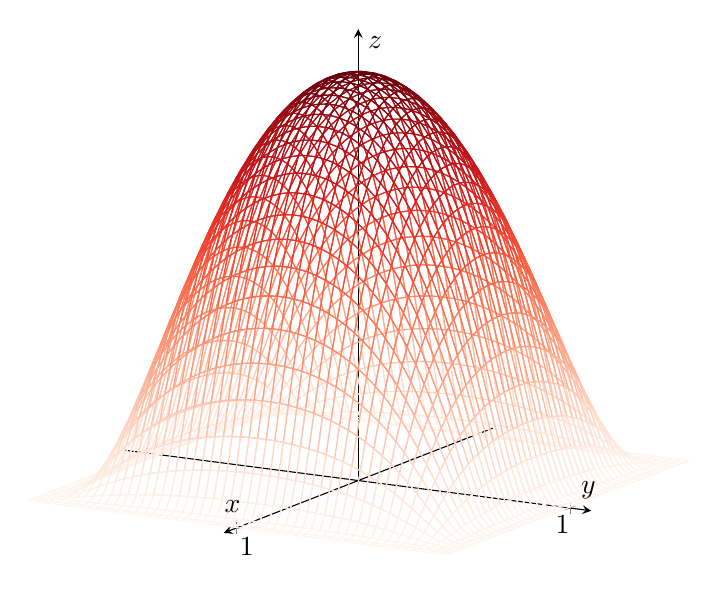
\begin{tikzpicture}
			\begin{axis}[
			view={120}{15},
			axis lines=middle,
			xlabel={$x$},
			xtick={1},
			xmin=-1.1,xmax=1.1,
			ylabel={$y$},
			ytick={1},
			ymin=-1.1,ymax=1.1,
			zlabel={$z$},
			ztick={0},
			zmin=0,zmax=0.15,
			width=0.9\textwidth,
			]
			\addplot3[mesh,samples=50,domain=-0.99:0.99,colormap/Reds]{exp(-1/(1-x^2))*exp(-1/(1-y^2))}; 
			\end{axis}
			\end{tikzpicture}
		\end{center}
		\caption{The graph of the function  $\Psi(x,y) = \psi(x)\psi(y)$, where $\psi$ is the single variable bump function from \cref{canonical-bump}.} \label{multivariable-bump-square-support-graph}
	\end{figure}
\end{exercise}

\begin{exercise} \label{multivariable-bump-round-support}
	Let $\psi : \R \to \R$ denote the single variable bump function from \cref{canonical-bump}. Then define $\alpha : \R^m \to \R$ by
	\[ \alpha(x_1, \dotsc, x_m) = \psi(x_1^2 + \dotsb + x_m^2). \]
	Show that $\alpha$ is a bump function supported on the closed unit ball $\bar{B}(0,1)$ with respect to the euclidean norm.  
\end{exercise}

\subsubsection*{Paths} \label{paths-multi}

\begin{definition}[Paths]
	Given $a, b \in \R^m$, a \emph{path} starting at $a$ and ending at $b$ is a continuous function $\gamma : [0, 1] \to \R^m$ such that $\gamma(0) = a$ and $\gamma(1) = b$. 
	\begin{itemize}
		\item We say that $\gamma$ is \emph{smooth} if it is the restriction to $[0,1]$ of a smooth function $(-\epsilon, 1+\epsilon) \to \R^m$ for some $\epsilon > 0$. This means that we can talk about the iterated derivatives $\gamma^{(k)}(t)$ not just for $t \in (0,1)$, but also for $t = 0, 1$. 
		\item We say that $\gamma$ is \emph{inside} or \emph{contained in} an open subset $U$ of $\R^m$ if $\gamma(t) \in U$ for all $t \in [0,1]$.
	\end{itemize}
\end{definition}

We met straight line paths between any two points of $\R^m$ in \cref{straight-line-path}, and then in \cref{convex}, we defined a subset $S \subseteq \R^m$ to be convex by requiring that all straight line paths between pairs of points of $S$ are inside $S$. 

\begin{exercise}
	Check that the straight line path between any two points in $\R^m$ is smooth. 
\end{exercise} 

\begin{exercise}[Slowing down smooth paths] \label{slowing-down-paths}
	Suppose $\gamma$ is a smooth path in $\R^m$. Show that there exists a smooth path $\gamma_{\text{slow-start}}$ with the same start and end as $\gamma$ and the same image as $\gamma$, such that 
	\[ \gamma_{\text{slow-start}}^{(k)}(0) = 0 \]
	for all $k \geq 1$. Then show that there also exists a smooth path $\gamma_{\text{slow-stop}}$ with the same start and end as $\gamma$ and the same image as $\gamma$, such that 
	\[ \gamma_{\text{slow-stop}}^{(k)}(1) = 0 \]
	for all $k \geq 1$. 
	\begin{hint}
		To slow down the start of the path, modify the ``infinitely flat'' function of  \cref{infinitely-flat} to find a function $f : \R \to \R$ such that $f^{(k)}(0) = 0$ for all $k \geq 0$ and $f(1) = 1$, and then consider $\gamma_{\text{slow-start}} = \gamma \circ f$. 
	\end{hint}
\end{exercise}

\begin{definition}[Concatentation of paths] \label{concatenation-paths}
	If $\gamma_1$ and $\gamma_2$ are paths in $\R^m$ and $\gamma_2$ starts where $\gamma_1$ ends, we define their \emph{concatenation} $\gamma_1 \star \gamma_2 : [0,1] \to \R^m$ as follows.
	\[ (\gamma_1 \star \gamma_2)(t) = \begin{cases} \gamma_1(2t) & \text{if } t \leq 1/2 \\ \gamma_2(2t-1) & \text{if } t > 1/2 \end{cases} \]
	In other words, $\gamma_1 \star \gamma_2$ ``travels along $\gamma_1$ at twice the speed,'' and then ``travels along $\gamma_2$ at twice the speed.''
\end{definition}

Observe that if $\gamma_1$ and $\gamma_2$ are both inside $U$, then $\gamma_1 \star \gamma_2$ is also inside $U$. However, even if $\gamma_1 \star \gamma_2$ are both smooth, their concatenation need not be. To concatenate smoothly, we can use the following. 

\begin{exercise}[Smooth concatenation] \label{smooth-concatenation-paths}
	Suppose $\gamma_1$ and $\gamma_2$ are smooth paths in $\R^m$ and $\gamma_2$ starts where $\gamma_1$ ends. Using the notation of \cref{slowing-down-paths,concatenation-paths}, show that
	\[ \gamma = \gamma_{1,\text{slow-stop}} \star \gamma_{2,\text{slow-start}} \]
	is smooth. 
\end{exercise}

\begin{exercise} \label{smoothly-path-connected}
	Suppose $U$ is a connected open subset of $\R^m$. Show that, for any pair of points $a, b \in U$, there exists a smooth path inside $U$ starting at $a$ and ending at $b$. 
	\begin{hint}
		Use \cref{smooth-concatenation-paths} and the first part of \cref{constant-iff-derivative-zero-connected}. 
	\end{hint}
\end{exercise}
	
	\chapter{Manifolds}

Roughly speaking, a ``manifold'' is a locally flat geometric object without pre-ordained local coordinate systems. Before we formalize what we mean by this, it's useful to philosophize a bit. First of all, let's think about what ``locally flat'' means. Consider, for example, the surface of the earth. On the one hand, we know that it's a sphere (approximately, at least). On the other hand, we also know from personal experience that the curvature of the earth is irrelevant in situations where everything of concern is within a few miles of us. The earth looks flat. It is in this sense that the surface of the earth is ``locally flat.'' 

When we have such a locally flat geometric object, it's often useful to introduce ``local coordinate systems.'' For example, we talk about things being ``in front of'' us or being ``behind'' us in our everyday lives, despite the fact that, if you go far enough forward, you'll eventually end up behind where you started! In other words, ``in front of'' and ``behind'' make no sense if we're thinking globally (ie, if we're thinking at the level of the entirety of the earth). They only make sense ``locally,'' but despite that, they're incredibly useful notions in everyday life. Similar considerations apply with ``left'' and ``right.''

It's also useful to allow local coordinate systems to change depending on the situation we're in. Returning to the example of ``in front of'' and ``behind,'' notice that these notions don't refer to absolute directions: if you turn 90$^\circ$ in some direction, what was ``in front of'' you before you turned isn't ``in front of'' you anymore. After your $90^\circ$ turn, there's now a new useful notion of ``in front of.'' In other words, changing the situation you're in has made a different local coordinate system useful.

Let's now return to the sentence we started with, that ``manifolds are locally flat geometric objects without pre-ordained local coordinate systems.'' We'll see below how to formalize ``locally flat'' mathematically. The way we'll avoid having pre-ordained local coordinate systems is by remembering \emph{all possible choices} of local coordinate systems! 

It's also worth remarking that this chapter marks a somewhat significant turning point in our meditation of derivatives and tangents. We began \cref{single} with the observation that we could formalize our intuitive idea of ``tangent line'' using  derivatives. In the next chapter, we'll see that, in the abstract setting of manifolds, we can formalize the idea of ``tangent vector,'' and then use it to define an even further generalization of the derivative. 

\section{Definition of a manifold}

At this point, we will need to use the language of topological spaces. If you've seen metric spaces but not topological spaces, you should skim through \cref{topological-spaces-basics} (in particular, at least \cref{topological-space-definition,metric-to-topological,continuous-definition,open-map-definition,homeomorphism-definition}).

\subsection{Charts}

Throughout this section, let $X$ be a topological space.\index{topological space} Recall that we want for $X$ to be ``locally flat.'' Formally, this means that we can cover $X$ with open subsets, each of which is ``flat'' in the sense that it is homeomorphic to an open subset of $\R^n$. Notice that, if we remember not just the fact that each open subset $U$ in that cover is homeomorph\emph{ic} to $\R^n$, but the actual homeomorph\emph{ism}, then we can transfer the usual coordinate system on $\R^n$ through the homeomorphism onto $U$. In other words, a homeomorphism between $U$ and an open subset of $\R^n$ tells us both that $U$ is ``flat,'' and gives us a coordinate system on $U$. This is precisely what's accomplished by the following definition. 

\begin{definition}[Chart] \index{chart}
	A \emph{chart} on $X$ is a pair $(U, \phi)$ consisting of an open subset $U \subseteq X$ and a continuous, open\index{open!open map}, and injective function $\phi : U \to \R^n$ for some $n$. 
	\begin{itemize}
		\item The integer $n$ is called the \emph{dimension} of the chart, and write $\dim (U,\phi)$ to denote it. 
		\item The function $x$ is called the \emph{coordinate function} of the chart. 
		\item If $a \in X$, we say that the chart $(U,\phi)$ \emph{contains} $a$ if $a \in U$. If $(U,\phi)$ contains $a$ and $\phi(a) = 0$, we say that $(U,\phi)$ is \emph{centered at} $a$. 
		\item For all $i = 1, \dotsc, n$, we define $\phi_i := \pi_i \circ \phi$. For any $a \in U$, the real numbers $\phi_1(a), \dotsc, \phi_n(a)$ are called the \emph{coordinates of $a$ with respect to the chart  $(U,\phi)$}.\index{coordinates}
	\end{itemize} 
\end{definition}

\begin{example} \label{polar-representation}
	Let $X = \R^2$ and let $U$ denote $\R^2$ minus the non-negative $x$-axis. In other words, 
	\[ U = \{(x,y) : x < 0 \text{ or } y \neq 0 \}. \]
	Let $\phi : U \to \R^2$ be the function which sends a point $p$ to its polar representation $\phi(p) = (r(p), \theta(p))$, where $r(p) = |p|$ and $\theta(p)$ is the angle in radians strictly between 0 and $2\pi$ formed between $p$ and the non-negative real axis. Let us show that $(U, \phi)$ is a chart. 
	
	Observe that $\phi$ is injective, we have
	\[ \phi(U) = \{ (r, \theta) : r > 0, \theta \in (0, 2\pi) \}, \]
	and the inverse function of $\phi$ is given by  $\phi^{-1}(r,\theta) = (r\cos \theta, r\sin\theta)$. Clearly $\phi^{-1}$ is continuous. In fact, it is even \'etale, since 
	\[ \det (\phi^{-1})'(r, \theta) = \det \begin{bmatrix} \cos \theta & -r\sin\theta \\ \sin\theta & r\cos \theta \end{bmatrix} = r^2 \neq 0 \]
	on $\phi(U)$, so the inverse function theorem \ref{inverse-function-theorem} tells us that $\phi^{-1}$ is open. This means that $\phi$ is continuous as well, proving that $(U, \phi)$ is a chart. 
	
	Notice that the chart $(U, \phi)$ contains the point $(1,1)$. We calculate the coordinates of $(1,1)$ with respect to this chart by evaluating $\phi(1,1)$. We find
	\[ \rho(1,1) = (\sqrt{1^2 + 1^2}, \arctan(1)) = (\sqrt{2}, \pi/4). \]
	In other words, $\phi$ outputs precisely the polar representation of $(1,1)$. 
\end{example}

\begin{remark} \label{recentering-chart}
	If $(U,\phi)$ is a chart on $X$ and $a \in U$  is a point, we can ``recenter the chart at $a$'' by replacing $\phi$ with the function $\tilde{\phi}$ given by $\tilde{\phi}(x) = \phi(x) - \phi(a)$. In other words, if $\tilde{\phi} = \phi - \phi(a)$, then $(U, \tilde{\phi})$ is also a chart, and we have $\tilde{\phi}(a) = 0$.
\end{remark}

\subsection{Compatibility of charts}

Charts formalize the idea of local coordinate systems; the following formalizes the idea of \emph{changing} local coordinate systems. 

\begin{definition}[Transition function] \label{transition-map} \index{transition function}
	Suppose $(U, \phi)$ and $(V, \psi)$ are charts on $X$. The \emph{transition function} from $(U, \phi)$ to $(V, \psi)$ is the function $\psi \circ \phi^{-1}$.
	\[ \begin{tikzcd}
	\phi(U \cap V) \ar{r}{\phi^{-1}} & U \cap V \ar{r}{\psi} & \psi(U \cap V)
	\end{tikzcd} \]
	Notice that the domain $\phi(U \cap V)$ is an open subset of $\R^m$ for $m = \dim(U, \phi)$ and the codomain $\psi(U \cap V)$ is an open subset of $\R^n$ for $n = \dim(V, \psi)$. In other words, $\psi \circ \phi^{-1}$ is precisely the kind of function whose derivative we studied in \cref{multi}. 
\end{definition}

\begin{definition}[Compatibility of charts] \index{compatibile} \label{compatibility}
	The two charts $(U, \phi)$ and $(V, \psi)$ on $X$ are \emph{smoothly compatible}, or just \emph{compatible}, if the transition map $\psi \circ \phi^{-1}$ from $(U, \phi)$ to $(V, \psi)$ and the transition map $\phi \circ \psi^{-1}$ from $(V, \psi)$ to $(U, \phi)$ are smooth. 
\end{definition}

\begin{example} \label{cube-not-compatible}
	Let $\id : \R \to \R$ denote the identity map and let $\phi : \R \to  \R$ denote the map $\phi(x) = x^3$. Both maps are homeomorphisms, so $(\R, \id)$ and $(\R, \phi)$ are charts. However, these two charts are not compatible. The transition function from $(\R, \id)$ to $(\R, \phi)$ is 
	\[ \begin{tikzcd} \R = \id(\R) \ar{r}{\id^{-1}} & \R \ar{r}{\phi} & \phi(\R) = \R, \end{tikzcd} \]
	which is just $\phi$, which is in fact smooth. However, in the other direction, the transition function is 
	\[ \begin{tikzcd} \R = \phi(\R) \ar{r}{\phi^{-1}} & \R \ar{r}{\phi} & \id(\R) = \R, \end{tikzcd} \]
	which is the function $\phi^{-1}(x) = \sqrt[3]{x}$. In other words, the transition function from $(\R, \phi)$ to $(\R, \id)$ is not even differentiable. 
\end{example}

\begin{exercise}
	Determine whether or not each of the following charts $(U, \phi)$ is compatible with $(\R, \id)$.
	\begin{enumerate}[(a)]
		\item $U = \R$ and $\phi(x) = 2x$.
		\item $U = \R$ and $\phi(x) = -x$. 
		\item $U = \R$ and $\phi(x) = x|x|$. 
		\item $U = \R$ and $\phi(x) = -x^3$. 
		\item $U = (-\pi/2, \pi/2)$ and $\phi(x) = \tan(x)$. 
		\item $U = (0, \infty)$ and $\phi(x) = \ln(x)$. 
		\item $U = \R$ and $\phi(x) = x^5$. 
	\end{enumerate}
	Use these examples to formulate a conjecture for determining when a chart $(U, \phi)$ on $\R$ is compatible with $(\R, \id)$. Then prove your conjecture. 
\end{exercise}

\begin{example} \label{polar-compatible-with-identity}
	Let $\id : \R^2 \to \R^2$ denote the identity map and $\phi : U \to \R^2$ the polar representation map from \cref{polar-representation}. The two charts $(\R^2, \id)$ and $(U, \rho)$ are compatible. To see this, observe that the transition function from $(U, \phi)$ to $(\R^2, \id)$ is the function
	\[ \begin{tikzcd} \phi(U) \ar{r}{\phi^{-1}} & U \ar{r}{\id} & \id(U) = U, \end{tikzcd} \]
	which is just $\phi^{-1}$. We saw in \cref{polar-representation} that $\phi^{-1}$ is given explicitly by \[ \phi^{-1}(r, \theta) = (r\cos\theta, r\sin\theta), \]
	which is a smooth function. Going the other way, the transition function from $(\R^2, \id)$ to $(U, \phi)$ is precisely $\phi$. 
	\[ \begin{tikzcd} U = \id(U) \ar{r}{\id^{-1}} \ar{r} & U \ar{r}{\phi} & \phi(U) \end{tikzcd} \]
	As we saw in \cref{polar-representation}, the map $\phi^{-1}$ is \'etale, so its inverse function $\phi$ is smooth by \cref{ck-stable-inversion}. Thus both transition functions are smooth, so the two charts are compatible. 
\end{example}

\begin{exercise}
	Show that two charts $(U,\phi)$ and $(V, \psi)$ are compatible if and only if the transition function from $(U, \phi)$ to $(V,\psi)$ is smooth and \'etale. 
\end{exercise}

\begin{exercise}
	Suppose $(U, \phi)$ is a chart and $a \in X$ is a point. Consider the recentered chart $(U, \tilde{\phi})$ where $\tilde{\phi} = \phi - \phi(a)$, as in \cref{recentering-chart}. Show that $(U, \phi)$ and $(U, \tilde{\phi})$ are compatible. 
\end{exercise}

\begin{remark} \label{compatibility-not-equivalence-relation}
	An important cautionary observation is that compatibility of charts is \emph{not} an equivalence relation on the set of all charts. It is certainly reflexive and symmetric, but it fails to be transitive. For example, let $\phi(x) = x^3$ and then consider the three charts $(\R, \id), (\R \setminus \{0\}, \phi)$, and $(\R, \phi)$. The first two are compatible with each other, and the second two are compatible with each other, but the first and third are \emph{not} compatible with each other (cf.  \cref{cube-not-compatible}). 
\end{remark}

\begin{exercise} \label{dimension-well-defined}
	Suppose $(U, \phi)$ and $(V, \psi)$ are compatible charts and that the intersection $U \cap V$ is nonempty. Show that $\dim(U,\phi) = \dim(V,\psi)$. 
	\begin{hint}
		Fix a point $a \in U \cap V$, and consider the derivative of the transition function $\psi \circ \phi^{-1}$ at $\phi(a)$. 
	\end{hint}
\end{exercise}

\subsection{Atlases and manifolds}

\begin{definition}[Atlas] \index{atlas} \index{atlas!maximal atlas} \index{maximal atlas|see {atlas, maximal atlas}}
	An \emph{atlas} on $X$ is a collection $\mathscr{A}$ of compatible charts such that covers $X$. In other words, a collection $\mathscr{A}$ of charts is an atlas if every pair of charts in $\mathscr{A}$ is compatible, and \[ \bigcup_{(U, \phi) \in \mathscr{A}} U = X. \]
	If $\mathscr{A}'$ is also an atlas and $\mathscr{A}' \subseteq \mathscr{A}$, we say that $\mathscr{A}'$ is a \emph{sub-atlas} of $\mathscr{A}$. An atlas is \emph{maximal} if there is no strictly larger atlas containing it.
\end{definition}

\begin{exercise}[Existence and uniqueness of maximal atlases] \label{existence-maximal-atlas}
	Prove that every atlas $\mathscr{A}$ is contained in a unique maximal atlas.\index{atlas!maximal atlas} 
	\begin{hint}
		Let $\mathscr{A}'$ be the set of all charts that are compatible with all of the charts in $\mathscr{A}$. Prove that $\mathscr{A}'$ is an atlas (caution: keep \cref{compatibility-not-equivalence-relation} in mind). Then prove that it is maximal, and that it is the only maximal atlas containing $\mathscr{A}$. 
	\end{hint}
\end{exercise}

\begin{exercise}
	Suppose $\mathscr{A}$ and $\mathscr{A}'$ are two atlases on $X$. Let us say that $\mathscr{A}$ and $\mathscr{A}'$ are \emph{compatible} if the union $\mathscr{A} \cup \mathscr{A}'$ is an atlas. 
	\begin{enumerate}[(a)]
		\item  Show that the following are equivalent. 
		\begin{enumerate}[(i)]
			\item $\mathscr{A}$ and $\mathscr{A}'$ are compatible. 
			\item Each chart in $\mathscr{A}$ is compatible with every chart in $\mathscr{A}'$. 
			\item $\mathscr{A}$ is a sub-atlas of the unique maximal atlas that contains $\mathscr{A}'$. 
		\end{enumerate}
		\item Show that compatibility \emph{is} an equivalence relation on the set of all atlases on $X$.
	\end{enumerate} 
	Make sure you understand how the assertion made in part (b) above differs from the assertion in \cref{compatibility-not-equivalence-relation}. Compatibility of  \emph{charts} is not an equivalence relation, compatibility of \emph{atlases} is. 
\end{exercise}

This leads us to the following definition.

\begin{definition}[Manifold] \index{manifold} \index{smooth manifold|see {manifold}}
	A \emph{smooth manifold}, or just a \emph{manifold}, is a pair $(X, \mathscr{A}_X)$ where $X$ is a topological space and $\mathscr{A}_X$ is a maximal atlas. Often, we just write ``$X$'' in place of the pair $(X, \mathscr{A}_X)$. Sometimes the maximal atlas $\mathscr{A}_X$ is called the \emph{manifold structure} or the \emph{smooth structure} on $X$.
\end{definition}

\Cref{existence-maximal-atlas} tells us that any not-necessarily-maximal atlas on a topological space $X$ can be extended uniquely to a maximal atlas, thus giving $X$ the structure of a manifold. When constructing examples, we will usually give an explicit finite non-maximal atlas and then use \cref{existence-maximal-atlas} to extend it to a maximal atlas; it is difficult to describe maximal atlases explicitly, because there are many, many charts in maximal atlases. But it is often convenient for theorem statements and abstract proofs to assume that the atlas that the manifold comes equipped with is already maximal, which is why the definition is made the way it is.

\begin{unimportantremark}
	For any $k = 0, 1, 2, \dotsc, \infty$, we could define charts to be \emph{$C^k$-compatible} by requiring that the transition functions between them are $C^k$ (rather than smooth, as in \cref{compatibility}). This would lead to a definition of \emph{$C^k$-manifolds}. In these notes, we'll just stick to the $k = \infty$ case.  
\end{unimportantremark}

\subsection{Dimension}

\begin{definition}[Dimension] \index{dimension!of a manifold}
	Suppose $X$ is a manifold and $a \in X$ is a point. By \cref{dimension-well-defined}, there is a unique integer $n$ such that $\dim(U,\phi) = n$ for every chart $(U, \phi) \in \mathscr{A}_X$ containing $a$. This integer is called the \emph{dimension of $X$ at $a$}, and is denoted $\dim_a(X)$. If there exists a single integer $n$ such that $\dim_x(X) = n$ for all $x \in X$, we say that $X$ is \emph{equidimensional} and that the \emph{dimension of $X$} is $n$. 
\end{definition}

\begin{proposition}
	If the set $\N$ of natural numbers is given the discrete topology, the function $X \to \N$ given by $x \mapsto \dim_x(X)$ is continuous. In particular, if $X$ is a nonempty connected manifold, it must be equidimensional. 
\end{proposition}

\begin{proof}
	To show that $x \mapsto \dim_x(X)$ is continuous, we want to show that, for any natural number $n$, the set 
	\[ X_n = \{ x \in X : \dim_x(X) = n \} \]
	is an open subset of $X$. Suppose $a \in  X_n$. Let $(U, \phi)$ be a chart containing $a$. Then $\dim(U,\phi) = n$, and we have $\dim_x(X) = n$ for all $x \in U$. In other words, $U \subseteq X_n$. Thus, for every $a \in X_n$, there exists an open neighborhood of $a$ that is entirely contained inside $X_n$, so $X_n$ is open. 
	
	Now suppose $X$ is connected and $a \in X$. Let $n = \dim_a(X)$, so that $a \in X_n$. Then 
	\[ X \setminus X_n = \bigcup_{m \neq n} X_m \]
	is a union of open sets and is therefore also open. Thus $X_n$ is a nonempty subset of $X$ that is both open and closed. Since $X$ is connected, we conclude that $X = X_n$. In other words, $X$ is equidimensional of dimension $n$. 
\end{proof}

\section{Examples}

\subsection{First examples}

\subsubsection*{Euclidean space}

\begin{example} \label{natural-euclidean-atlas}
	The single chart $(\R^n, \id)$, where $\id : \R^n \to \R^n$ is the identity map, defines an atlas on $\R^n$. We can extend this to a maximal atlas, called the \emph{euclidean atlas} on $\R^n$. Unless explicitly specified otherwise, we always regard $\R^n$ as a manifold by equipping it with the euclidean atlas. The polar representation chart of  \cref{polar-representation,polar-compatible-with-identity} is an element of the euclidean atlas on $\R^2$. 
\end{example}

\begin{exercise}
	For any $r > 0$, let $\phi_r : \R \to \R$ be the function
	\[ \phi_r(t) = \begin{cases} t & \text{if } t \leq 0 \\ rt & \text{if } t > 0. \end{cases} \]
	Note that $\phi_r$ is continuous and strictly increasing (hence also injective and open, by \cref{strictly-monotone-iff-injective,strictly-monotone-implies-open}), so $(\R, \phi_r)$ is a chart. Note also that $\phi_1 = \id$. 
	\begin{enumerate}[(a)]
		\item Show that $\phi_s \circ \phi_r = \phi_{sr}$ and that $(\phi_r)^{-1} = \phi_{1/r}$. 
		\item Show that $(\R, \phi_r)$ and $(\R, \phi_s)$ are compatible if and only if $r = s$.
		\item Let $\mathscr{A}_r$ be the maximal atlas obtained by extending $(\R, \phi_r)$. What can you say about $\mathscr{A}_r$ and $\mathscr{A}_s$ if $r \neq s$? Are any of these the euclidean atlas? What can you conclude about the number of maximal atlases on $\R$?
	\end{enumerate}  
\end{exercise}

\begin{exercise} \label{euclidean-chart-characterization}
	Suppose $U$ is an open subset of $\R^n$ and $\phi : U \to \R^n$ is a function. Show that the pair $(U, \phi)$ is a chart in the euclidean atlas on $\R^n$ if and only if $\phi$ is injective, smooth, and \'etale.
\end{exercise}

\subsubsection*{Circles and spheres}

\begin{exercise}[The circle $S^1$] \index{s1@$S^1$|see {circle}} \index{circle} \label{circle-projection-atlas}
	Let $S^1$ denote the set of points in $\R^2$ along the unit circle. In other words,
	\[ S^1 = \{ (x, y) \in \R^2 : x^2 + y^2 = 1 \}. \]
	\begin{enumerate}[(a)]
		\item Do \cref{metric-subspace}. This shows that both ways that we might think to regard $S^1$ as a topological space are actually the same. 
		
		\item Let $U = S^1 \setminus \{(0,1)\}$. For a point $a \in S^1$, let $\phi(a)$ denote the $x$-coordinate of the point where the line $y = -1$ intersects the line passing through $(0,1)$ and $a$. This is sometimes called ``projection from the north pole.'' See \cref{circle-projection}. If $a = (x,y)$, find an explicit formula for $\phi(a)$ in terms of $x$ and $y$. 
		
		\begin{figure}
			\begin{center}
				\begin{tikzpicture}
				\begin{axis}[
				xmin=-1.5,xmax=1.5,
				ymin=-1.3,ymax=1.3,
				ytick={-1,1},
				xtick={-1,1},
				xticklabels={},
				yticklabels={},
				axis lines=middle,
				axis line style=lightgray,
				width=\textwidth,
				axis equal
				]
				
				\addplot[black,style=thick,-] expression[domain=-1:1,samples=200]{sqrt(1-x^2)}; 
				\addplot[black,style=thick,-] expression[domain=-1:1,samples=200]{-sqrt(1-x^2)};
				
				
				\addplot[red,<->] expression[domain=-0.1:0.95,samples=2]{-2.414*x+1}; 
				
				
				\addplot[black,<->] expression[domain=-1.5:1.5,samples=2]{-1};
				
				\node[label={85:{$(0,1)$}},color=white,draw=black,circle,fill,inner sep=2pt] at (axis cs:0,1) {}; 
				\node[label={0:{$a$}},color=black,draw=black,circle,fill,inner sep=2pt] at (axis cs:0.707,-0.707) {}; 
				\node[color=red,draw=red,circle,fill,inner sep=2pt] at (axis cs:0.8285,-1) {}; 
				
				\end{axis}
				\end{tikzpicture}
			\end{center}
			\caption{Given a point $a \in U = S^1 \setminus \{(0,1)\}$, we draw a line connecting $a$ to $(0,1)$, indicated in red. The point where that line intersects the line $y = -1$ (in black) is sometimes called the ``projection'' of $a$ from $(0,1)$ onto $\R \times \{-1\}$. The $x$-coordinate of this point is $\phi(a)$.}  \label{circle-projection}
		\end{figure}
		
		\item Show that $\phi : U \to \R$ is a homeomorphism.\index{homeomorphism} Thus $(U, \phi)$ is a chart on $S^1$. 
		\begin{hint} 
			Use geometry to write down a formula for the inverse function to $\phi$. 
		\end{hint}
		
		\item Let $V = S^1 \setminus \{(0,-1)\}$. For $a \in V$, let $\psi(a)$ denote the $x$-coordinate of the point where the line $y = 1$ intersects the line passing through $(0,-1)$ and $a$. Show that $\psi : V \to \R$ is also a homeomorphism. 
		
		\item Show that $(U, \phi)$ and $(V, \psi)$ are compatible charts. Thus $\mathscr{A} = \{(U, \phi), (V, \psi)\}$ is an atlas on $S^1$. Extending $\mathscr{A}$ to a maximal atlas $\mathscr{A}_{S^1}$, we have defined a manifold structure on $S^1$.
		
		\item Let $W = \{ (x,y) \in S^1 : x > 0 \}$ be the ``right half of the circle.'' If $\pi : W \to \R$ is the function $\pi(x,y) = y$, show that $(W,\pi)$ is a chart and that it is compatible with the two charts in the atlas $\mathscr{A}$ constructed above. Thus $(W, \pi) \in \mathscr{A}_{S^1}$. 
		
		\item Can you think of any other charts in the maximal atlas $\mathscr{A}_{S^1}$, besides the three discussed above?
		
		\begin{hint}
			There are many, many possibilities here. You could project other halves of the circle onto the $x$-axis or the $y$-axis, like in (f). More interestingly, you could also think about charts defined using trigonometric functions. 
		\end{hint}
	\end{enumerate}
\end{exercise}

\begin{exercise}[The $n$-sphere $S^n$] \label{sphere-projection-atlas} \index{sn@$S^n$|see {$n$-sphere}} \index{n-sphere@$n$-sphere}
	Let $S^n$ denote the set of points in $\R^{n+1}$ that have euclidean norm 1. Generalize \cref{circle-projection-atlas} and show that ``projection from the north pole'' and ``projection from the south pole'' define an atlas on $S^n$. 
\end{exercise}

\subsubsection*{Matrices and vector spaces}

\begin{example}[Matrices]
	There is an isomorphism of vector spaces $\phi : \mathscr{M}_{n \times m} \to \R^{mn}$\index{mnm@$\mathscr{M}_{n \times m}$} where, if $A \in \mathscr{M}_{n \times m}$ has entries $a_{i,j}$, then
	\[ \phi(A) = \begin{bmatrix} a_{1,1} \\ a_{1,2} \\ \vdots \\ a_{1,m} \\ a_{2,1} \\ \vdots \\ a_{n,m} \end{bmatrix}. \]
	If we endow $\mathscr{M}_{n \times m}$ with the canonical topology,\index{canonical topology} then $\phi$ is automatically a homeomorphism by \cref{linear-isomorphism-homeomorphism}.\index{homeomorphism} In other words, the single chart $(\mathscr{M}_{n \times m}, \phi)$ is an atlas on $\mathscr{M}_{n \times m}$. Extending it to a maximal atlas using \cref{existence-maximal-atlas}, we see that we can regard $\mathscr{M}_{n,m}$ as a manifold. It is $mn$-dimensional.  
\end{example}

The same process discussed above allows us to regard \emph{any} finite dimensional vector space as a manifold. 

\subsubsection*{Constructions}

\begin{exercise}[Graphs of continuous functions] \label{graphs-continuous}
	Suppose $U$ is an open subset of $\R^m$ and $f : U \to \R^n$ is a continuous function. 
	\begin{enumerate}[(a)]
		\item There are two ways we might think to regard $U \times \R^n$ as a topological space. One way is to use the product topology \ref{product-space}. The second way is to regard $U \times \R^n$ as a subset of $\R^m \times \R^n = \R^{m+n}$ and then give $U \times \R^n$ the subspace topology \ref{subspace-topology}. Show that these two topologies are the same. 
		
		\item Let $\Gamma = \{ (x,y) \in U \times \R^n : f(x) = y \}$ be the graph of $f$, regarded as a subspace of $U \times \R^n$. Show that the function $\pi : \Gamma \to \R^m$ given by $\pi(x,y) = x$ is continuous, injective, and open. 
	\end{enumerate}
	Thus the single chart $(\Gamma, \pi)$ defines an atlas on $\Gamma$. Extending this to a maximal atlas, we can regard $\Gamma$ as a manifold. 
\end{exercise}

\begin{exercise}[Open submanifolds] \label{open-submanifold}
	Let $X$ be a manifold and $U \subseteq X$ an open subset. Show that \[ \mathscr{A}_U = \{ (V,\phi) \in \mathscr{A}_X : V \subseteq U \} \]
	is a maximal atlas on $U$. We call $U$, equipped with this maximal atlas, an \emph{open submanifold} of $X$. 
\end{exercise}

\begin{exercise}[Product manifold]
	Let $X$ and $Y$ be manifolds. Let $\mathscr{A}$ be the set of charts of the form $(U \times V, \phi \times \psi)$, where $(U, \phi) \in \mathscr{A}_X$, $(V, \psi) \in \mathscr{A}_Y$, and $\phi \times \psi$ denotes the natural map $U \times V \to \R^m \times \R^n = \R^{m+n}$, where $m = \dim(U,\phi)$ and $n = \dim(V, \psi)$. Show that $\mathscr{A}$ is an atlas on $X \times Y$. We call $X \times Y$, equipped with the corresponding maximal atlas, the \emph{product manifold}. 
\end{exercise}

\subsection{M\"obius strip}

Let $B$ denote the box $[0,1] \times (0,1)$ inside $\R^2$, and let $\sim$ be the equivalence relation on $B$ generated by declaring $(0,y) \sim (1,1-y)$ for all $y \in (0,1)$. 
See \cref{mobius-box}. The equivalence class of a point $(x,y) \in B$ is denoted by $[x,y]$. Observe that every equivalence class contains either 1 or 2 elements. The \emph{M\"obius strip}\index{mobius strip@M\"obius strip} $M$ is the set of equivalence classes in $B$. In other words, we take the box $[0,1] \times (0,1)$ and ``glue'' its left and right edges, with a twist. If you've ever made a M\"obius strip out of paper, you can probably see that we've formalized exactly that same process. See \cref{mobius-box}, again.

\begin{figure}
	\begin{center}
	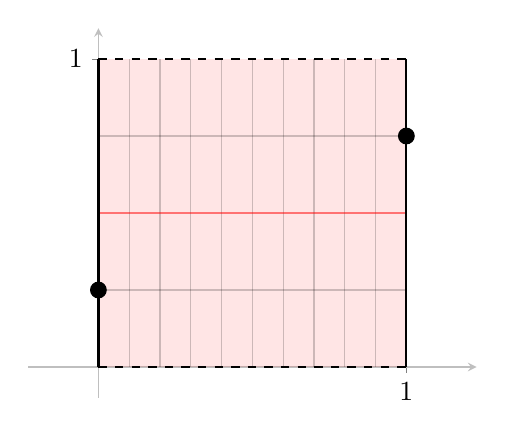
\begin{tikzpicture}
	\begin{axis}[
	xmin=-0.1,xmax=1.1,
	ymin=-0.1,ymax=1.1,
	ytick={1},
	xtick={1},
	xticklabels={1},
	yticklabels={1},
	axis lines=middle,
	axis line style=lightgray,
	axis equal,
	width=0.6\textwidth
	]
	
	\addplot[black, opacity=0.2, domain=0:1, samples=2] {0.25};
	\addplot[black, opacity=0.2, domain=0:1, samples=2] {0.75};
	
	\foreach \n in {1, ..., 9}
		\addplot +[mark=none, black, solid, opacity=0.2] coordinates {(0.1*\n, 0) (0.1*\n, 1)};
	
	\addplot[black, dashed, name path=top, domain=0:1, samples=2] {0};
	\addplot[black, dashed, name path=bottom, domain=0:1, samples=2] {1};
	\addplot [fill=red, fill opacity=0.1] 
	fill between[of=top and bottom];
	
	
	\addplot[red, thick, domain=0:1, samples=2, opacity=0.5] {0.5};
	\addplot +[mark=none, solid, thick, black] coordinates {(0, 0) (0, 1)};
	\addplot +[mark=none, solid, thick, black] coordinates {(1, 0) (1, 1)};
	
	\node[color=black,draw=black,circle,fill,inner sep=2pt] at (axis cs:0,0.25) {}; 
	\node[color=black,draw=black,circle,fill,inner sep=2pt] at (axis cs:1,0.75) {}; 
	\end{axis}
	\end{tikzpicture}
	
	\vspace{2em}
	
	
	\caption{Above is a picture of the box $B = [0,1] \times (0,1)$ and the equivalence relation $\sim$ described above. Geometrically, this equivalence relation identifies the vertical black line on the left of the box with the vertical black line on the right of the box, but ``with a twist.'' For example, the point $(0,1/4)$ on the left is identified with the point $(1,3/4)$ on the right. If we pick up the box and actually glue together the edges as indicated by the equivalence relation, we end up with the M\"obius strip as pictured below.} \label{mobius-box}
	
	\vspace{3em}
	
	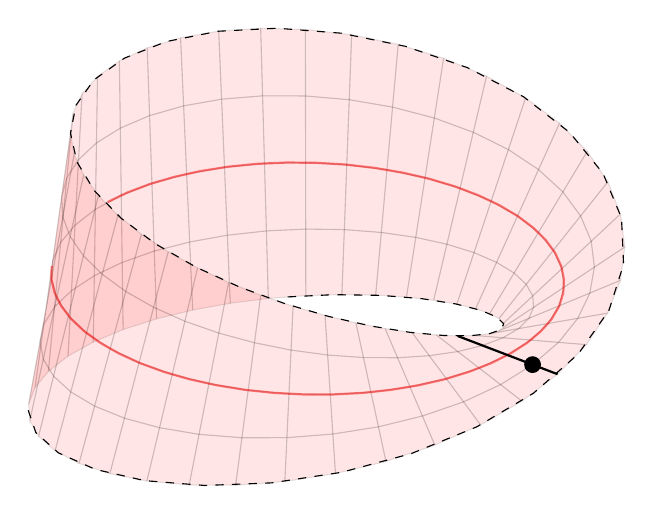
\begin{tikzpicture}
	\begin{axis}[
	hide axis,
	view={40}{40},
	width=\textwidth]
	
	\addplot3 [surf,
	red,
	opacity=0.1,
	faceted color=black,
	point meta=x,
	samples=40,
	samples y=5,
	z buffer=sort,
	domain=0:360,
	y domain=-0.5:0.5
	] (
	{(1+0.5*y*cos(x/2)))*cos(x)},
	{(1+0.5*y*cos(x/2)))*sin(x)},
	{0.5*y*sin(x/2)});
	
	% Center line
	\addplot3 [samples=50, domain=-145:180, samples y=0, red, thick, opacity=0.5
	] ({cos(x)},{sin(x)},{0});
	
	% Outside line
	\addplot3 [samples=50, domain=-135:495, samples y=0, black, dashed] (
	{(1+0.25*cos(x/2)))*cos(x)},
	{(1+0.25*cos(x/2)))*sin(x)},
	{0.25*sin(x/2)});
	
	% Glued line
	\addplot3 [samples=50,domain=-0.5:0.5,samples y=0, black, thick,
	] ({1+0.5*x},{0},{0});
	
	% Point
	\node[color=black,draw=black,circle,fill,inner sep=2pt] at (axis cs:1+1/8,0,0) {};
	\end{axis}
	\end{tikzpicture}
	\end{center}
\end{figure}

We regard $M$ as a topological space using the quotient topology, as in \cref{quotient-space}. To give $X$ the structure of a manifold, we will construct an atlas consisting of two charts. But, before proceeding with the formalism, let's describe the intuition. Imagine making a cut in the M\"obius strip corresponding to a vertical cut in the box $B$ (ie, a cut perpendicular to the central red circle in \cref{mobius-box}). Once we make such a cut, we can untwist the M\"obius strip and we're left with an open rectangle, which we can regard as an open subset of $\R^2$. In other words, we've defined a chart on $M$. The points along the cut are missing from this chart; but if we construct a second chart by making a second separate cut, we will have constructed two charts that cover $M$. 

Let's formalize this now. The easiest place to cut is the line along which we glued the M\"obius strip in the first place. In other words, we let \[ U = \{ [x, y] \in M : x \in (0,1) \} \] 
and let $\phi : U \to \R^2$ be the function $\phi([x,y]) = (x, y)$.

\begin{exercise} \label{first-chart-mobius}
	Show that $U$ is an open subset of $M$, and that the function $\phi : U \to \R^2$ is well-defined, continuous, injective, and open. 
\end{exercise}

\begin{solution}{\cref{first-chart-mobius}}
	Let $\pi : B \to M$ be the map $\pi(x,y) = [x,y]$. To show that $U = \{[x,y] \in M : x \neq 0,1\}$ is open, we use the definition of the quotient topology \cref{quotient-space}, which tells us that $U$ is an open subset of $M$ precisely when $\pi^{-1}(U)$ is an open subset of $B$. But \[ \pi^{-1}(U) = B^\circ = (0,1) \times (0,1) \] is an open subset of $B$, so $U$ is open in $M$. 
	
	The facts that $\phi : U \to \R^2$ is well-defined and injective follow immediately from the observation that every equivalence class in $U$ has exactly one element. To see that $\phi$ is continuous, suppose $W$ is an open subset of $\R^2$. We want to show that $\phi^{-1}(W)$ is open in $U$, ie, that $\pi^{-1}(\phi^{-1}(W))$ is open in $B$. But $\pi^{-1}(\phi^{-1}(W)) = B^\circ \cap W$ is an intersection of two open subsets, so it is also open. 
	
	To see that $\phi$ is open, suppose $W$ is an open subset of $U$. We want to show that $\phi(W)$ is an open subset of  $\R^2$. But notice that $\phi(W) = \pi^{-1}(W)$, and we know that $\pi^{-1}(W)$ is open in $B$ by the definition of open subsets in the quotient topology. Moreover, $\phi(W) \subseteq B^\circ$, so $\phi(W)$ is an open subset of $B^\circ$. Since $B^\circ$ is open in $\R^2$, we conclude that $\phi(W)$ is open in $\R^2$. 
\end{solution}

The second chart is a bit harder to describe mathematically, but the intuitive idea is the same. We'll cut the M\"obius strip along the line corresponding the vertical line $x = 1/2$ in $B$. Formally, let \[ V = \{ [x, y] \in M : x \neq 1/2 \} \] and let $\psi : V \to  \R^2$ be the function defined by 
\[ y([x, y]) = \begin{cases} (x, y) & \text{if } x < 1/2 \\ (x-1, 1-x) & \text{if } x > 1/2 \end{cases} \]

\begin{exercise} \label{second-chart-mobius}
	Show that $V$ is also an open subset of $M$, and that $\psi : V \to \R^2$ is well-defined, continuous, injective, and open. 
\end{exercise}

\begin{solution}{\cref{second-chart-mobius}}
	Let $\pi : B \to M$ be the map $\pi(x, y) = [x,y]$ again. Observe that $\pi^{-1}(V) = \{ (x,y) \in B : x \neq 1/2 \}$  is an open subset of $B$ (even though it is not an open subset of $\R^2$), so by definition of the quotient topology, $V$ is an open subset of $M$. 
	
	Let us check that $\psi$ is well-defined. Most equivalence classes have just one element, and $\psi$ is clearly well-defined on those equivalence classes. Equivalence classes with two points are of the form $[0,y] = [1,1-y]$ for some $y \in (0,1)$. Observe that 
	\[ \psi([1,1-y]) = (0,1-(1-y)) = (0,y) = \psi([0,y]), \]
	which shows that $\psi$ is well-defined on the equivalence classes with two elements as well. 
	The verification that $\psi$ is continuous, injective, and open will be left to the reader. 
\end{solution}

\begin{exercise} \label{mobius-charts-compatible}
	Show that $(U, \phi)$ and $(V, \psi)$ are compatible.
\end{exercise}

\begin{solution}{\cref{mobius-charts-compatible}}
	Observe that the transition function $\psi \circ  \phi^{-1}$ from $(U,\phi)$ to $(V,\psi)$ is the composite 
	\[ \begin{tikzcd} \phi(U \cap V) \ar{r}{\phi^{-1}} & U \cap V \ar{r}{\psi} & \psi(U \cap V) \end{tikzcd} \]
	given by 
	\[ (\psi \circ \phi^{-1})(x,y) = \psi([x,y]) = \begin{cases} (x,y) & \text{if } x < 1/2 \\ (x-1, 1-y) & \text{if } x > 1/2 \end{cases} \]
	which is clearly smooth, and 
	\[ (\psi \circ \phi^{-1})'(x,y) = \begin{cases} \begin{bmatrix} 1 & 0 \\ 0 & 1 \end{bmatrix} & \text{if } x < 1/2 \\ \begin{bmatrix} 1 & 0 \\ 0 & -1 \end{bmatrix} & \text{if } x > 1/2 \end{cases} \]
	which shows that $\psi \circ \phi^{-1}$ is \'etale. Thus the two charts are compatible. 
\end{solution}

Thus $\mathscr{A} = \{(U, \phi), (V, \psi)\}$ is an atlas on the M\"obius strip $M$. Letting $\mathscr{A}_M$ denote the corresponding maximal atlas, we obtain the structure of a manifold on $M$.

\begin{exercise}
	Fix a constant $c \in [0,1)$, and let $U_c$ be the subset of $M$ where we've cut out the vertical line $x = c$. Show that $U_c$ is an open subset of $M$. Write down a formula for a well-defined function $\phi_c : U_c \to \R^2$ which is continuous, injective, and open; the image of $\phi_c$ should be an open box in $\R^2$, and you should recover the function $\phi$ above when $c = 0$, and the function $\psi$ when $c = 1/2$. Then show that $(U_c, \phi_c) \in \mathscr{A}_M$ for all $c \in [0,1)$. 
\end{exercise}

\subsection{More quotient examples}

Here are some more examples of manifolds you probably recognize which you probably recognize. 

\begin{exercise}[Cylinder] \label{cylinder}
	Let $S$ denote the infinite vertical strip $[0,1] \times \R$ inside $\R^2$, and let $\sim$ be the equivalence relation generated by $(0,y) \sim (1,y)$ for all $y \in \R$. Let $C$ be the corresponding quotient space. Describe an atlas on $C$. 
\end{exercise}

\begin{exercise}[Torus] \label{torus} \index{torus}
	Let $B$ denote the box $[0,1] \times [0,1]$ inside $\R^2$ and let $\sim$ denote the equivalence relation generated by $(x,0) \sim (x,1)$ and $(0,y) \sim (1,y)$ for all $x,y \in [0,1]$. The \emph{torus} $T$ is defined to be the corresponding quotient space. Describe an atlas on $T$. 
\end{exercise}

% TODO: Torus picture

Sometimes quotient spaces can be very difficult to visualize directly; the only way to have geometric intuition in these cases is to remember the space we started with before quotienting, and the equivalence relation we defined on it. 

\begin{exercise}[Projective line] \label{rp1} \index{projective line} \index{p1@$\bbP^1$|see {projective line}}
	Let $S^1$ denote the circle as in \cref{circle-projection-atlas}. Define an equivalence relation $\sim$ on $S^1$ which identifies antipodal points; in other words, every point on $S^1$ is declared to be equivalent to the point that is diametrically opposite it. The \emph{projective line} $\bbP^1$ is defined to be the corresponding quotient space. Describe an atlas on $\bbP^1$. 
\end{exercise}

\begin{exercise}[Projective plane] \label{rp2} \index{projective plane} \index{p2@$\bbP^2$|see {projective plane}}
	Let $S^2$ denote the 2-sphere as in \cref{sphere-projection-atlas}. Define an equivalence relation $\sim$ on $S^2$ which identifies antipodal points. The \emph{projective plane} $\bbP^2$ is defined to be the corresponding quotient space. Describe an atlas on $\bbP^2$. 
\end{exercise}

\subsection{Submanifolds}

We now define submanifolds. Recall that, if $(U, \phi)$ is a chart, then $\phi_i = \pi_i \circ \phi$ denotes the corresponding $i$th coordinate function. 

\begin{definition} \label{submanifold}
	Suppose $S$ is a subset of a manifold $X$. Then $S$ is a \emph{submanifold} of $X$ if there exist charts $(U, \phi) \in \mathscr{A}_X$ covering $S$ such that 
	\[ S \cap U = \{ x \in U :  \phi_{k+1}(x) = \phi_{k+2}(x) = \dotsb = \phi_n(x) = 0 \} \]
	for some non-negative integer $k \leq \dim(U,x)$. Such a chart $(U,\phi)$ is called a \emph{slice chart} for $S$, or an \emph{adapted chart} for $S$, and the integer $k$ is called the \emph{dimension of $S$ in $(U,\phi)$}. 
\end{definition}

Intuitively, the definition says that, in the coordinate system on $U$ induced by the chart $(U, \phi)$, the subset $S \cap U$ should look like an open subset of a coordinate hyperplanes (specifically, the coordinate hyperplane where $x_{k+1} = x_{k+2} = \dotsb = x_n = 0$, ie, the $(x_1, x_2, \dotsc, x_k)$-hyperplane). See \cref{submanifold-definition-picture}. 

\begin{figure}
	\begin{center}
	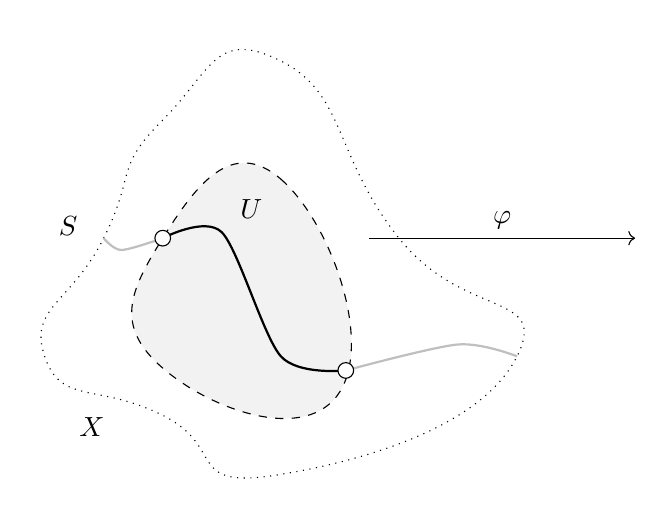
\begin{tikzpicture}[scale=1.5]
	\draw[dotted] plot [smooth cycle, tension=1] coordinates { (0,0) (0.5,1) (1,2) (2,2.5) (3,1) (4,0) (2,-1) (1, -0.5) };
	\draw[dashed,fill=gray,fill opacity=0.1] plot [smooth cycle, tension=1] coordinates { (1,1) (2,1.5) (2.5,-0.3) (1, -0.1) };
	
	
	\draw[thick, lightgray, solid] plot [smooth] coordinates {(0.5,1) (0.65,0.9) (1,1)};
	\draw[thick, black, solid] plot [smooth] coordinates {(1,1) (1.5,1.05) (2,0) (2.55,-0.12)};
	\draw[thick, lightgray, solid] plot [smooth] coordinates {(2.55,-0.12) (3.5,0.1) (4,0)};
	\node[color=white,draw=black,circle,fill,inner sep=2pt] at (1,1) {}; 
	\node[color=white,draw=black,circle,fill,inner sep=2pt] at (2.55,-0.12) {}; 
	
	\node at (0.4,-0.6) {$X$};
	\node at (0.2,1.1) {$S$};
	\node at (1.75,1.25) {$U$};
	\draw[black,->] (2.75,1) -- node[above] {$\phi$} (5,1);
	\end{tikzpicture}
	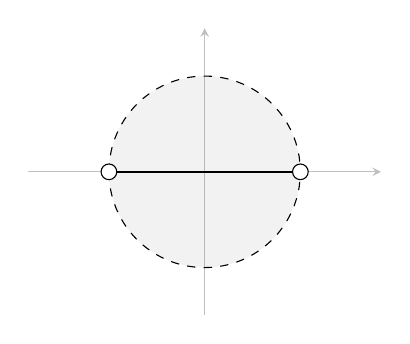
\begin{tikzpicture}
	\begin{axis}[
	xmin=-1.5,xmax=1.5,
	ymin=-1.5,ymax=1.5,
	ytick={0},
	xtick={0},
	axis lines=middle,
	axis line style=lightgray,
	width=0.5\textwidth,
	axis equal
	] 
	
	
	\addplot[black,dashed] expression[name path=a,domain=-1:1.15,samples=200]{sqrt(1-x^2)};
	\addplot[black,dashed] expression[name path=b,domain=-1:1.15,samples=200]{-sqrt(1-x^2)};
	
	\addplot[fill=gray, fill opacity=0.1]
	fill between[of=a and b,soft clip={domain=-1:1.15}];
	
	\addplot +[mark=none,black,thick,solid,-] coordinates {(-1,0) (1, 0)};
	\node[color=white,draw=black,circle,fill,inner sep=2pt] at (axis cs:-1,0) {}; 
	\node[color=white,draw=black,circle,fill,inner sep=2pt] at (axis cs:1,0) {}; 
	\end{axis}
	\end{tikzpicture}
	\end{center}
	\caption{Suppose $X$ is a manifold (depicted above as an amorphous blob) and $S$ is a subset (depicted above as a squiggly line passing through the blob). Then $S$ is defined to be a \emph{submanifold} of $X$ if $S$ can be covered by charts $(U, \phi)$ such that, under $\phi$, the set $S \cap U$ corresponds to a coordinate hyperplane in $\R^n$. In the picture above, the map $\phi : U \to \R^2$ pulls the squiggle $S \cap U$ taut onto the $x$-axis inside $\R^2$. } \label{submanifold-definition-picture}
\end{figure}

We'll justify the word ``submanifold'' in a moment by showing that submanifolds are actually manifolds in their own right (cf. \cref{submanifolds-are-manifolds}). But first, let's discuss some examples. The intuition you should carry into these examples is roughly that, if a subset ``looks smooth'' (ie, doesn't have any ``pointy'' parts), it should be a submanifold. 

\begin{example}
	Consider the set $S = \{ (x,0) \in \R^2 : -1 < x < 1 \}$ inside $\R^2$. In other words, $S$ is the open interval $(-1,1)$ along the $x$-axis inside $\R^2$. Then $S$ is a submanifold. Indeed, let $U$ be the open box $(-1,1) \times (-1,1)$ inside $\R^2$, and $\phi : U \to \R^2$ the inclusion map. Then $(U, \phi)$ is a chart in the euclidean atlas on $\R^2$, $\phi_2(x,y) = y$, and 
	\[ \{ (x,y) \in U : \phi_2(x, y) = 0 \} = \{ (x,y) \in U : y = 0 \} = S = S \cap U \]
	so $(U,\phi)$ is adapted to $S$ and $S$ has dimension 1 in $(U,\phi)$. 
\end{example}

\begin{example}
	Consider the parabola \[ S = \{ (x, y) \in \R^2 : y = x^2, x \in \R \}. \] This ``looks smooth,'' so it should be a submanifold. Let's see how. It is sufficient to produce a chart $(\R^2, \phi)$ with the property that 
	\[ S = \{ (x,y) \in \R^2 : \phi_2(x,y) = 0 \}. \]
	This means we should take $\phi_2(x,y) = x^2 - y$. Then $\phi_1$ should be a smooth function $\phi_1 : \R^2 \to \R$ such that $\phi = (\phi_1, \phi_2)$ is injective and \'etale. In other words, we want the Jacobian matrix 
	\[ \phi'(x,y) = \begin{bmatrix} \dfrac{\partial \phi_1}{\partial x} & \dfrac{\partial \phi_1}{\partial y} \\ 2x & -1 \end{bmatrix} \]
	to always be invertible. The easiest way to guarantee this is to take $\phi_2(x,y) = x$, which makes $\det \phi'(x,y) = 1$. Moreover, the function $\phi(x,y) = (x, x^2 - y)$ is injective, since if $\phi(x_1, y_1) = \phi(x_2,y_2)$, then $(x_1, x_1^2 - y_1) = (x_2, x_2^2 - y_2)$, and looking at the first coordinates shows that $x_1 = x_2$, and finally looking at the first coordinates shows that $y_1 = y_2$. In other words, $(\R^2, \phi)$ is a slice chart for $S$ in the euclidean atlas, so $S$ is a submanifold of $\R^2$. 
\end{example}

\begin{comment}
	The subset  
	\[ S = \{(x,y) : y = |x|, x \in \R \} \]
	is ``pointy'' and does \emph{not} define a submanifold of $\R^2$. To see this formally, suppose there exists a chart $(U, \phi)$ on $\R^2$ that is adapted to $S$ and contains the origin. By making $U$ smaller, we can assume that $U$ is a box of the form $(-\epsilon, \epsilon) \times (-\epsilon, \epsilon)$. Then $S \cap U$ is neither all of $U$ nor just a point, so it must be that $S$ has codimension 1 in $(U, \phi)$. In other words, 
	\[ S \cap U = \{ (x,y) : \phi_1(x,y) = 0 \}. \]
\end{comment}

\begin{exercise}
	Show that each of the following is a submanifold of $\R^2$. 
	\begin{enumerate}[(a)] 
		\item The $y$-axis. 
		\item The open interval $(-1,1)$ along the $x$-axis.
		\item The line $y = x$.  
		\item The curve $y = x^3$. 
	\end{enumerate}
\end{exercise}

\begin{exercise} \label{circle-submanifold}
	Show that the unit circle $S^1$ is a submanifold of $\R^2$. 
	\begin{hint}
		Let $U = \{(x,y) \in S^1 : x > 0 \}$ and let $\phi(x,y) = (x,x^2+y^2-1)$. See \cref{circle-submanifold-picture}. Show that $(U, \phi)$ is a chart that is adapted to $S^1$. But this one chart does not cover the circle, so then find more charts like this one that cover the circle. 
	\end{hint}
	\begin{figure}
		\begin{center}
			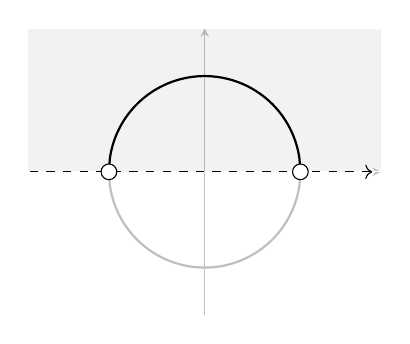
\begin{tikzpicture}
			\begin{axis}[
			xmin=-1.5,xmax=1.5,
			ymin=-1.5,ymax=1.5,
			ytick={0},
			xtick={0},
			yticklabels={},
			axis lines=middle,
			axis line style=lightgray,
			width=0.5\textwidth,
			axis equal
			] 
			
			
			\addplot[white] expression[name path=c,domain=-2:2,samples=2]{1.5};
			\addplot[white] expression[name path=d,domain=-2:2,samples=2]{0};
			\addplot[fill=gray, fill opacity=0.1]
			fill between[of=c and d,soft clip={domain=-2:2}];
			
			\addplot[black,thick] expression[domain=-1:1,samples=200]{sqrt(1-x^2)};
			\addplot[lightgray,thick] expression[domain=-1:1,samples=200]{-sqrt(1-x^2)};
			
			\addplot +[mark=none,black,dashed,->] coordinates {(-2, 0) (1.75, 0)};
			
			\node[color=white,draw=black,circle,fill,inner sep=2pt] at (axis cs:-1,0) {}; 
			\node[color=white,draw=black,circle,fill,inner sep=2pt] at (axis cs:1,0) {}; 
			
			\end{axis}
			\end{tikzpicture}\hspace{1cm}
			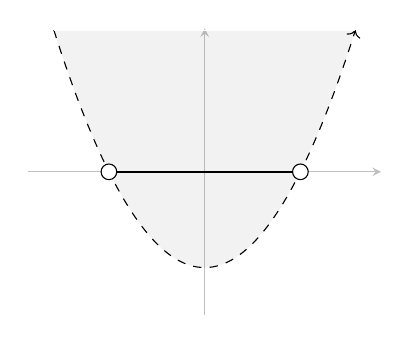
\begin{tikzpicture}
			\begin{axis}[
			xmin=-1.5,xmax=1.5,
			ymin=-1.5,ymax=1.5,
			ytick={0},
			xtick={0},
			axis lines=middle,
			axis line style=lightgray,
			width=0.5\textwidth,
			axis equal
			] 
			
			
			\addplot[black,dashed,->] expression[name path=b,domain=-1.575:1.575,samples=200]{x^2-1};
			\addplot[white] expression[name path=a,domain=-1.575:1.575,samples=2]{1.575^2-1};
			\addplot[fill=gray, fill opacity=0.1]
			fill between[of=a and b,soft clip={domain=-2:2}];
			
			\addplot +[mark=none,black,thick,solid,-] coordinates {(-1, 0) (1, 0)};
			
			\node[color=white,draw=black,circle,fill,inner sep=2pt] at (axis cs:-1,0) {}; 
			\node[color=white,draw=black,circle,fill,inner sep=2pt] at (axis cs:1,0) {}; 
			\end{axis}
			\end{tikzpicture}
		\end{center}
		\caption{If $U = \{(x,y) : x > 0\}$ is the right half of the plane and $\phi : U \to \R^2$ is given by $\phi(x,y) = (x^2 + y^2 - 1, x)$, then $(U, \phi)$ is a chart on $\R^2$ that transforms the picture on the left into the picture on the right. The vertical axis on the left turns into the parabola on the right. The top half of the circle on the left turns into the horizontal line segment on right. The vertical axis on the left stays remains the vertical axis on the right.}  \label{circle-submanifold-picture}
	\end{figure}
\end{exercise}

\begin{exercise} \label{graphs-smooth-single}
	Show that the graph of a smooth function $f : \R \to \R$ is a submanifold of $\R^2$. 
\end{exercise}

\begin{caution}
	Sometimes, a subspace that is a manifold can fail to be a submanifold. For example, you might notice that we showed in \cref{graphs-continuous} that the graph of a \emph{continuous} function $\R \to \R$ is a subspace of $\R^2$ and is also a manifold; and then we showed in \cref{graphs-smooth-single} that the graph of a \emph{smooth} function $\R \to \R$ is a submanifold of $\R^2$. And indeed, the graphs of continuous-but-not-smooth functions provide examples of subspaces that are manifolds but not submanifolds. 
\end{caution}

\begin{exercise}
	Let $C$ be the cylinder from \cref{cylinder} and let $L$ be the line \[ L = \{ [1/2, y] \in C : y \in \R \}. \] Show that $L$ is a submanifold of $C$. 
\end{exercise}

We now make good on our promise of proving that submanifolds are in fact manifolds. The proof is a little long because there are a lot of details to check, but there are no real tricks or surprises. 

\begin{proposition} \label{submanifolds-are-manifolds}
	Let $S$ be a submanifold of a manifold $X$. Suppose $(U, \phi) \in \mathscr{A}_X$ is adapted to $S$ and $S$ has dimension $k$ in $(U, \phi)$. Let $\phi|_S : S \cap U \to \R^k$ be the function defined by 
	\[ \phi|_S(p) = (\phi_1(p), \dotsc, \phi_k(p)). \]
	Regarding $S$ as a topological space using the subspace topology, the pair $(S \cap U, \phi|_S)$ is a chart on $S$, and the set of all charts of this form is an atlas on $S$. Thus $S$ becomes a manifold if we equip it with the corresponding maximal atlas $\mathscr{A}_S$. Finally, for any $x \in S$, if $(U, \phi) \in \mathscr{A}_X$ is a slice chart for $S$ containing $x$ such that $S$ has dimension $k$ in $(U,\phi)$, then $\dim_x(S) = k$. 
\end{proposition}

\begin{proof}
	Observe that, by definition, $\phi|_S$ is the composite
	\[ \begin{tikzcd}
	S \cap U \ar[hookrightarrow]{r} & U \ar{r}{\phi} & \R^n \ar{r}{\pi} & \R^{k}
	\end{tikzcd} \]
	where the first map is the inclusion, and the final map $\pi : \R^n \to \R^{k}$ projects onto the first $k$ coordinates (ie, $\pi(x_1, \dotsc, x_n) = (x_{1}, \dotsc, x_k)$). Each of these maps is continuous, so the composite $x|_S$ is continuous as well. The proof that $\phi|_S$ is injective is left as an exercise (cf. \cref{submanifolds-are-manifolds-details}). 
	
	Let us show that $\phi|_S$ is open. By definition of the subspace topology \ref{subspace-topology}, every open subset of $S \cap U$ is of the form $S \cap V$ where $V$ is an open subset of $U$. Suppose $a \in  S \cap V$. We want to show that $\phi|_S(a)$ is an interior point of $\phi|_S(S \cap V)$. Since $V$ is open in $U$ and $\phi : U \to \R^n$ is an open map, we know that $\phi(a)$ is an interior point of $\phi(V)$, ie, there exists $\epsilon > 0$ such that every point of $\R^n$ within $\epsilon$ of $\phi(a)$ is inside $\phi(V)$. We claim that the $\epsilon$ ball around $\phi|_S(a)$ is contained in $\phi|_S(S \cap V)$. In other words, suppose we have $y = (y_{1}, \dotsc, y_k) \in \R^{k}$ such that $|y - \phi|_S(a)| < \epsilon$. We will show that $y \in \phi|_S(S \cap V)$. 
	
	Notice that, since $(U,\phi)$ is a slice chart for $S$, the vector $\phi(a) \in \R^n$ is the same as $\phi|_S(a) \in \R^{k}$ except that for some trailing zeroes. Let $\iota : \R^k \to \R^n$ be the map that concatenates vectors in $\R^{n-k}$ with a string of $n-k$ zeroes. In other words, 
	\[ \iota(y_1, \dotsc, y_k) = (y_1, \dotsc, y_k, \overbrace{0, \dotsc, 0}^{n-k \text{ times}}). \]
	Thus $\phi(a) = \iota(\phi|_S(a))$. Now by the definition of the either the euclidean or the max norm, we see that $|\iota(y) - \phi(a)| = |y - \phi|_S(a)|$, which means that $|\iota(y) - \phi(a)| < \epsilon$. This means that $\iota(y) \in \phi(V)$ due to our choice of $\epsilon$. Since $\phi$ is injective, there exists a unique $b \in V$ such that $\phi(b) = \iota(y)$. This means that the first $k$ coordinates of $b$ are zero, so $b \in S \cap U$ since $(U, \phi)$ is a slice chart for $S$. Moreover
	\[ \phi|_S(b) = \pi(\phi(b)) = \pi(\iota(y)) = y \]
	which shows that $y \in \phi|_S(S \cap V)$. 
	
	Next up, suppose $(U, \phi)$ and $(U', \phi')$ are both charts in $\mathscr{A}_X$ that are adapted to $S$. We want to show that $(S \cap U, \phi|_S)$ and $(S \cap U', \phi'|_S)$ are compatible. If $S \cap U \cap U'$ is empty, there is nothing to do, so we assume that $S \cap U \cap U'$ is nonempty. Let $k$ and $k'$ be the dimensions of $S$ in the two charts $(U, \phi)$ and $(U', \phi')$, respectively. 
	
	The proof of compatibility is encapsulated by the following diagram. 
	\[ \begin{tikzcd}
	\phi|_S(S \cap U \cap U') \ar{r}{(\phi|_S)^{-1}} \ar{d}[swap]{\iota} & S \cap U \cap U' \ar[hookrightarrow]{d} \ar{r}{\phi'|_S} & \phi'|_S(S \cap U \cap U') \\
	\phi(U \cap V) \ar{r}{\phi^{-1}} & U \cap V \ar{r}{\phi} & \phi'(U \cap V) \ar{u}[swap]{\pi'}
	\end{tikzcd} \]
	Here $\iota$ denotes the ``concatenate with $n-k$ trailing zeroes'' map, and $\pi'$ is the ``project onto the first $k'$ coordinates'' map. You should stare at the above diagram until you've convinced yourself that it ``commutes,'' ie, that the result of following any two paths of arrows that start and end at the same place ends up being the same. (The fact that the square on the left of the diagram commutes is because $(U, \phi)$ is a slice chart for $S$, and the fact that square on the right commutes is by definition of the function $\phi'|_S$.)
	
	In other words, the diagram tells us that the transition function $\phi'|_S \circ (\phi|_S)^{-1}$ is equal to $\pi' \circ (\phi' \circ \phi^{-1}) \circ \iota$. Since $(U,\phi)$ and $(U', \phi')$ are compatible, we know that $\phi' \circ \phi^{-1}$ is smooth. Thus the transition function $\phi'|_S \circ (\phi|_S)^{-1}$ is smooth. 
	
	Since $S$ is a submanifold, we know that it can be covered by charts in $X$ that are adapted to $S$. Thus we've just shown that the set
	\[ \mathscr{A} = \{ (S \cap U, \phi|_S) : (U, \phi) \in \mathscr{A}_X \text{ is a slice chart for } S \} \]
	is an atlas on $S$. The assertion about $\dim_x(S)$ follows immediately. 
\end{proof}

\begin{exercise} \label{submanifolds-are-manifolds-details}
	Show that $\phi|_S$ is injective. 
\end{exercise}

\begin{exercise}
	We now have produced two maximal atlases on the unit circle: one we produced in \cref{circle-projection-atlas}, and then another is produced by \cref{circle-submanifold,submanifolds-are-manifolds}. Show that these two maximal atlases are the same. 
\end{exercise}

We've used the word ``submanifold'' once before, in \cref{open-submanifold} where we defined ``open submanifolds.'' Let us now show that this earlier usage of the word ``submanifold'' was justified and does not produce any conflicts with our new definitions.  

\begin{exercise}[``Open submanifolds are submanifolds''] \label{open-submanifolds-are-submanifolds}
	Suppose $X$ is a manifold and $U$ is an open subset. Show that $U$ is a submanifold (in the sense of \cref{submanifold}), and that the maximal atlas on $U$ constructed by \cref{submanifolds-are-manifolds} is equal to the atlas described in \cref{open-submanifold}. 
	\begin{hint}
		Show that a chart $(V, \phi) \in \mathscr{A}_X$ is a slice chart for $U$ if and only if $V \subseteq U$. 
	\end{hint}
\end{exercise}

Here is another property you would hope would be true. 

\begin{exercise}[``Submanifolds of submanifolds are submanifolds'']
	Let $X$ be a manifold, $S$ a submanifold of $X$, and $T$ a submanifold of $S$. Show that $T$ is a submanifold of $X$. 
\end{exercise}

Finally, here is a result that lets us produce many manifolds by considering graphs of smooth functions on euclidean space. 

\begin{proposition} \label{graphs-smooth}
	Suppose $U$ is an open subset of $\R^m$ and $f : U \to \R^n$ is smooth. Then the graph 
	\[ \Gamma = \{ (x,y) \in U \times \R^n : f(x) = y \} \]
	is a submanifold of $U \times \R^n$. 
\end{proposition}

\begin{proof}
	Consider the function $\phi : U \times \R^n \to \R^{m+n}$ given by $\phi(x,y) = (x,f(x)-y)$. Then $\phi$ is injective, since if $\phi(x, y) = (a,b)$, then clearly $x = a$ and $y = f(a)-b$, so any input to $\phi$ is determined by its input. It is also clear that $\phi$ is smooth. If we compute the derivative, we find that  
	\[ \phi'(x,y) = \begin{bmatrix} 
	1 & 0 & \dotsb & 0 & 0 & 0 & \dotsb & 0 \\ 
	0 & 1 & \dotsb & 0 & 0 & 0 & \dotsb & 0 \\
	\vdots & \vdots & \ddots & \vdots & \vdots & \vdots & \ddots & \vdots \\
	0 & 0 & \dotsb & 1 & 0 & 0 & \dotsb & 0 \\ 
	\partial_1 f_1(x) & \partial_2 f_1(x) & \dotsb & \partial_m f_1(x) & -1 & 0 & \dotsb & 0 \\
	\partial_1 f_2(x) & \partial_2 f_2(x) & \dotsb & \partial_m f_2(x) & 0 & -1 & \dotsb & 0 \\
	\vdots & \vdots & \ddots & \vdots & \vdots & \vdots & \ddots & \vdots \\
	\partial_1 f_n(x) & \partial_2 f_n(x) & \dotsb & \partial_m f_n(x) & 0 & 0 & \dotsb & -1
	\end{bmatrix} = \begin{bmatrix} I_n & 0 \\ f'(x) & -I_m \end{bmatrix}, \]
	where $I_r$ denotes the $r \times r$ identity matrix. In other words, the Jacobian matrix $\phi'(x,y)$ is a lower triangular $(n+m)\times(n+m)$ matrix with determinant $(-1)^m$. Thus $\phi$ is \'etale, so $(U \times \R^n, \phi)$ is a chart in the euclidean atlas on $U \times  \R^n$. It is evidently a slice chart for $\Gamma$, proving that $\Gamma$ is a submanifold of $U \times \R^n$. 
\end{proof}

\begin{exercise}
	Suppose $U$ is an open subset of $\R^m$ and $f : U \to \R^n$ is a smooth function. We have discussed two maximal atlases on the graph $\Gamma$ of $f$. One was discussed in \cref{graphs-continuous}, and the other arises by combining \cref{graphs-smooth,submanifolds-are-manifolds}. How do these atlases compare?
\end{exercise}

\subsection{Submersion theorem}

We now have a very important result which let us produce lots of examples of submanifolds of euclidean space out of smooth functions (in the sense of \cref{smooth-multi}). This result goes by many names, including the ``regular level set theorem,'' the ``preimage theorem'' and the ``submersion theorem.'' We will later generalize this result. 

\begin{theorem}[Submersion theorem] \label{submersion-theorem-local}
	Suppose $U$ is an open subset of $\R^m$ and $f : U \to \R^n$ is smooth and submersive. Then $S = f^{-1}(b)$ is a submanifold of $U$ of dimension $m-n$ for any $b \in f(U)$. 
\end{theorem}

\begin{proof}
	By replacing $f$ with the function $x \mapsto f(x)-b$, we can assume without loss of generality that $b = 0$. Fix $a \in S$. We want to find a slice chart for $S$ containing $p$. We know that $f$ is submersive at $a$, which means that the $n \times m$ matrix $f'(a)$ has a non-vanishing $n \times n$ minor. By permuting the coordinates (cf. \cref{permutation-submanifold}), we can assume that it is the $n \times n$ minor on the far right of $f'(a)$ that does not vanish. In other words, we can assume without loss of generality that  
	\begin{equation} \label{derivative-non-vanishing-minor} 
	\det \begin{bmatrix} \partial_{m-n+1} f_1(a) & \dotsb & \partial_{m-n+1} f_1(a) \\ \vdots & \ddots & \vdots \\ \partial_{m} f_n(a) & \dotsb & \partial_{m} f_n(a) \end{bmatrix} \neq 0. 
	\end{equation} Consider the function $\phi : U \to \R^m$ such that, if $x = (x_1, \dotsc, x_m) \in U$, then
	\[ \phi(x) = (x_1, \dotsc, x_{m-n}, f_{1}(x), \dotsc, f_n(x)). \]
	Then 
	\[ \phi'(x) = \begin{bmatrix}
	1 & 0 & \dotsb & 0 & 0 & \dotsb & 0 \\
	0 & 1 & \dotsb & 0 & 0 & \dotsb & 0 \\
	\vdots & \vdots & \ddots & \vdots & \vdots & \ddots & \vdots \\
	0 & 0 & \dotsb & 1 & 0 & \dotsb & 0 \\
	\partial_1 f_{1}(x) & \partial_2 f_{1}(x) & \dotsb & \partial_n f_{1}(x) & \partial_{n+1} f_{1}(x)& \dotsb & \partial_m f_{1}(x) \\ 
	\vdots & \vdots & \ddots & \vdots & \vdots & \ddots & \vdots \\
	\partial_1 f_{n}(x) & \partial_2 f_{n}(x) & \dotsb & \partial_n f_{n}(x) & \partial_{n+1} f_{n}(x)& \dotsb & \partial_m f_{n}(x) \\ 
	\end{bmatrix}. \]
	In other words, the $(m-n) \times (m-n)$ submatrix on the top left is the identity matrix, the $(m-n) \times n$ submatrix on the top right of $\phi'(x)$ is all zeroes, and the bottom $n \times m$ submatrix is precisely $f'(x)$. This means that $\det \phi'(x)$ is equal, up to sign, to the determinant of the $n \times n$ in the bottom right, ie, the $n \times n$ minor on the far right of $f'(x)$. We know from \cref{derivative-non-vanishing-minor} that this minor is nonzero when $x = a$, so $\phi$ is \'etale at $a$. 
	
	Since $f$ is smooth, so is $\phi$, so there exists an open neighborhood $V$ of $a$ such that $\phi|_V$ is \'etale. By the inverse function theorem \ref{inverse-function-theorem}, we can replace $V$ with a smaller open neighborhood of $a$ in order to further assume that $\phi|_V$ is injective. Then \cref{euclidean-chart-characterization} tells us that $(V, \phi)$ is a chart in the euclidean atlas which contains $a$. Moreover, 
	\[ S \cap V = \{ x \in V : f(x) = 0 \} = \{ x \in V : \phi_{m-n+1}(x) = \dotsb = \phi_{m-n+1}(x) = 0 \} \]
	because $\phi_{m-n+j} = f_j$ for all $j = 1, \dotsc, n$. This shows that $(V,\phi)$ is a slice chart for $S$, and that $S$ has dimension $m-n$ at $a$ in $\R^m$. 
\end{proof}

\begin{exercise} \label{permutation-submanifold}
	Suppose $\sigma$ is a permutation of the set $\{1, \dotsc, m\}$. Let $f_\sigma : \R^m \to \R^m$ be the function which ``permutes the coordinates of elements of $\R^m$ according to $\sigma$,'' ie, 
	\[ f_\sigma(x_1, \dotsc, x_m) = (x_{\sigma(1)}, \dotsc, x_{\sigma(m)}). \]
	Show that a subset $S$ is a submanifold of $\R^m$ if and only if $f_\sigma(S)$ is a submanifold of $\R^m$. 
\end{exercise}

\begin{exercise}
	Recall from \cref{circle-projection-atlas,sphere-projection-atlas} that the $n$-sphere $S^n$ is defined by
	\[ S^n = \{ x \in \R^{n+1} : |x|_2 = 1 \}. \]
	Use the submersion theorem to show that $S^n$ is a submanifold of $\R^{n+1}$. 
\end{exercise}

\begin{exercise} \label{torus-equation}
	Let $T$ be the torus inside $\R^3$ centered around the $z$-axis where the distance from the origin to the center of the tube is $R$, the radius of the tube is $r$, and $0 < r < R$. Find a smooth submersive map $f : U \to \R$ where $U$ is an open subset of $\R^3$ and \[ T = \{ (x,y,z) \in U : f(x,y,z) = 0 \}. \]
	Applying the submersion theorem \ref{submersion-theorem-local}, we conclude that $T$ is a submanifold of $\R^3$. 
	\begin{hint}
		See \cref{torus-slice}. 
	\end{hint}
	\begin{figure}[ht]
		\begin{center}
			\begin{tikzpicture}
			\begin{axis}[
			xmin=-4.5,xmax=4.5,
			ymin=-2,ymax=3,
			ytick={0},
			xtick={-3,3},
			xticklabels={$-R$,$R$},
			yticklabels={},
			axis lines=middle,
			axis line style=lightgray,
			width=\textwidth,
			axis equal,
			ylabel={$z$}
			]
			
			\addplot[black,style=thick] expression[domain=2:4,samples=200]{sqrt(1 - (x-3)^2)};
			\addplot[black,style=thick] expression[domain=2:4,samples=200]{-sqrt(1 - (x-3)^2)};
			\addplot[black,style=thick] expression[domain=-4:-2,samples=200]{sqrt(1 - (x+3)^2)};
			\addplot[black,style=thick] expression[domain=-4:-2,samples=200]{-sqrt(1 - (x+3)^2)};
			
			\node[label={45:$(x,y,z)$},color=black,draw=black,circle,fill,inner sep=2pt] at (axis cs:3.5,0.866025) (A) {};
			\node[color=black,draw=black,circle,fill,inner sep=1pt] at (axis cs:3,0) (B) {};
			\node[color=black,draw=black,circle,fill,inner sep=1pt] at (axis cs:3.5,0) (C) {};
			\node[label={$r$}] at (axis cs:3.1,0.3) {};
			
			\draw[black] (B) -- (A) -- (C) -- (B);
			\end{axis}
			\end{tikzpicture}
		\end{center}
		\caption{A slice of the torus $T$ from \cref{torus-equation} along a plane that is perpendicular to the $xy$-plane and contains the $z$-axis.}  \label{torus-slice}
	\end{figure}
\end{exercise}

\section{Smooth functions}

% TODO: Fix notation

We will now define what it means for a function between two manifolds to be smooth. Roughly, the idea is that we know what smooth means on open subsets of $\R^n$, and we just use charts to transfer the definition to arbitrary manifolds. 

Recall that in \cref{multi} we saw that the case when the codomain is $\R$ was the most important. The same will be true here. You may find that the number of definitions of ``smooth'' gets slightly out of hand; if you do, just remember that, whenever multiple definitions of ``smooth'' make sense for the objects in question, they'll all agree. 

\subsection{Smooth real-valued functions}

\subsubsection*{Definition of smoothness for real-valued functions}

\begin{definition}[Smooth real-valued function] \label{smooth-real-valued} \index{smooth}
	Let $X$ be a manifold. A function $f : X \to \R$ is said to be \emph{smooth} if, for any chart $(U, x) \in \mathscr{A}_X$, the function $f \circ x^{-1}$ is smooth.
	\[ \begin{tikzcd} x(U) \ar{r}{x^{-1}} & U \ar{r}{f} & \R \end{tikzcd} \]
\end{definition}

There are two disconcerting things about this definition. First, there is the issue that checking smoothness of a particular function seems next to impossible: the maximal atlas $\mathscr{A}_X$ will have \emph{many, many} charts, some that we may not even know about, and the definition makes it seem like we need to check smoothness on all of them! Thankfully, we don't need to check on all possible charts. As soon as we check smoothness on any atlas, even if it's not maximal, we're done. 

\begin{lemma} \label{smooth-real-valued-local}
	Let $X$ be a manifold and $f : X \to \R$ a function. Suppose that there exists an atlas $\mathscr{A} \subseteq \mathscr{A}_X$ such that $f \circ x^{-1}$ is smooth for any $(U, x) \in \mathscr{A}$. Then $f$ is smooth. 
\end{lemma}

\begin{proof}
	Suppose $(V, y) \in \mathscr{A}_X$. For any $(U, x) \in \mathscr{A}$, we have maps as follows.
	\[ \begin{tikzcd} y(U \cap V) \ar{r}{y^{-1}} \ar{d}[swap]{x \circ y^{-1}} & U \cap V \ar{r}{f} & \R \\ x(U \cap V) \ar[bend right]{ur}[swap]{x^{-1}} \end{tikzcd} \]
	Since $(V, y)$ and $(U, x)$ are both elements of the maximal atlas $\mathscr{A}_X$, we know that the transition function $x \circ y^{-1}$ is smooth. Since $(U, x) \in \mathscr{A}$, we know by assumption that $f \circ x^{-1}$ is smooth. Thus \[ f \circ y^{-1} = (f \circ x^{-1}) \circ (x \circ y^{-1}) \]
	is a smooth function $y(U \cap V) \to \R$. 
	
	Now note that, since $\mathscr{A}$ is an atlas, its charts cover all of $X$, so
	\[ \bigcup_{(U,x) \in \mathscr{A}} y(U \cap V) = y(V). \]
	Since $f \circ y^{-1}$ is smooth when restricted to each the open subset $y(U \cap V)$ for all $(U, x) \in \mathscr{A}$, we conclude that $f \circ y^{-1}$ must be smooth on all of $y(V)$.
\end{proof}

The second disconcerting thing is the following. Suppose $U \subseteq \R^m$ is an open subset and $f : U \to \R$ is a function. On the one hand, we defined what it means for $f$ to be smooth back in \cref{smooth-multi}. On the other hand, we can regard $U$ as an open submanifold of $\R^n$ (cf. \cref{open-submanifold}) and then \cref{smooth-real-valued} gives us another definition of what it means for $f$ to be smooth. A priori, it could be that these definitions conflict. Thankfully, they do not. 

\begin{exercise}
	Suppose $U \subseteq \R^m$ is an open subset and $f : U \to \R$ is a function. Show that $f$ is smooth in the sense of \cref{smooth-multi} if and only if it is smooth in the sense of \cref{smooth-real-valued}. 
	\begin{hint}
		You might find \cref{smooth-real-valued-local} useful. 
	\end{hint}
\end{exercise}

From here on out, we'll use the fact that these two definitions of smoothness coincide without comment. 

\subsubsection*{Combining smooth real-valued functions}

\begin{definition}
	If $X$ is a manifold, we write $\O(X)$ for the set of smooth functions $X \to \R$. 
\end{definition}

Here is the standard set of stability properties we would want. 

\begin{exercise} \label{smooth-real-valued-stable}
	\begin{enumerate}[(a)]
		\item Show that $\O(X)$ is a vector space. 
		\item If $f, g \in \O(X)$, show that $fg \in \O(X)$ also. 
		\item If $f \in \O(X)$ and $f(x) \neq 0$ for all $x$, show that $1/f \in \O(X)$ also. 
		\begin{hint}
			You might decide to do part (d) first, and then use it to prove (c). Or not, you could also just prove (c) directly. 
		\end{hint}
		\item Suppose $f \in \O(X)$, $U$ is an open subset of $\R$, $g : U \to \R$ is smooth, and $f(X) \subseteq U$. Show that $g \circ f \in \O(X)$. 
	\end{enumerate}
\end{exercise}

\begin{unimportantremark}
	if you've taken abstract algebra, you might be interested to notice that the first two stability properties in \cref{smooth-real-valued-stable} show that $\O(X)$ is an $\R$-algebra (ie, that it is simultaneously a commutative ring and a vector space, and that these two structures are ``compatible'' with each other). 
\end{unimportantremark}

\subsubsection*{Smooth approximations of characteristic functions of compact subsets \starred}

Here is a generalization of \cref{constant-compact-zero-outside-neighborhood} which proves, roughly speaking, that we can find a smooth approximation of the characteristic function of a compact subset of a manifold. You may want to look at \cref{compact-topological-space} for the definition of compactness for topological spaces. 

\begin{proposition} \label{smooth-approximation-characteristic-compact}
	Suppose $K$ is a compact subset of a manifold $X$ and $U$ is an open neighborhood of $K$. Then there exists a smooth function $f \in \O(X)$ such that $0 \leq f(x) \leq 1$ for all $x \in \R$, $f(x) = 1$ for all $x \in K$, and $f(x) = 0$ for all $x \notin U$. 
\end{proposition}

\begin{proof}
	Suppose $(V, x)$ is a chart containing some $p \in K$. Recentering, we can assume that $x(p) = 0$ (cf. \cref{recentering-chart}). By shrinking $V$, we can assume that $\bar{V} \subseteq U$ (cf. \cref{smooth-approximation-characteristic-compact-details}). Then $x(V)$ is an open neighborhood of $0 = x(p) \in \R^n$, so there exists $\epsilon > 0$ such that $B(0, \epsilon) \subseteq x(V)$. Let $\psi : \R^n \to \R$ be a bump function supported on $\overline{B}(0, \epsilon)$ (cf. \cref{multivariable-bump-round-support}). Then $\psi \circ x$ is a smooth function on $V$ (cf. \cref{smooth-approximation-characteristic-compact-details}) which is supported entirely inside $V$ (namely, on $x^{-1}(\overline{B}(0,\epsilon))$), and is zero everywhere else on $V$. Define $f_p : X \to \R$ by
	\[ f_p(x) = \begin{cases} \psi \circ x & \text{if } x \in V \\ 0 &  \text{if } x \notin V. \end{cases} \]
	Then $f_p$ is smooth (cf. \cref{smooth-approximation-characteristic-compact-details}), and it is strictly positive on an open neighborhood $V_p$ of $p$ contained inside $U$.  
	
	We can construct such a function $f_p$ for every $p \in K$. Since $K$ is compact, there exist finitely many $p_1, \dotsc, p_n \in K$ such that $K \subseteq V_{p_1} \cup \dotsb \cup V_{p_n}$. Thus $f_{p_1} + \dotsb + f_{p_n}$ is strictly positive on $K$, and zero outside $U$. Since $K$ is compact, there exists $\delta > 0$ such that $f_{p_1} + \dotsb + f_{p_n} \geq \delta$ on $K$ (cf. \cref{smooth-approximation-characteristic-compact-details}). Let $g$ be a bridging function such that $g(x) = 1$ for $x \geq \delta$ and $g(x) = 0$ for $x \leq 0$ (cf. \cref{bridge-function}), and then set $f = g \circ (f_{p_1} + \dotsb + f_{p_n})$.
\end{proof}

\begin{exercise} \label{smooth-approximation-characteristic-compact-details}
	Fill in the missing details in the above proof. 
	\begin{enumerate}[(a)]
		\item Prove that we can ``shrink $V$ in order to assume that $\bar{V} \subseteq U$.''
		\item Modify the bump function of \cref{multivariable-bump-round-support} so that it has support $\overline{B}(0, \epsilon)$. 
		\item Explain why $\psi \circ x$ is a smooth function $V \to \R$. 
		\item Explain why $f_p$ is a smooth function $X \to \R$. 
		\item If $h : K \to \R$ is a continuous function such that $h(x) > 0$ for all $x \in K$, show that there exists $\delta > 0$ such that $h(x) \geq \delta$ for all $x$. 
		
		\begin{hint}
			Let $\delta = \inf\{ h(x) : x \in K \}$ and recall the extreme value theorem. 
		\end{hint}
	\end{enumerate}
\end{exercise}

% TODO: Partitions of unity

\subsection{Smooth functions between manifolds}

Here is a definition that may look a bit terrifying at first. 

\begin{definition}[Smoothness] \label{smooth-between-manifolds} \index{smooth}
	Suppose $X$ and $Y$ are manifolds and $f : X \to Y$ is a function. Then $f$ is \emph{smooth} if, for every chart $(V, y) \in \mathscr{A}_Y$ and every chart $(U, x) \in \mathscr{A}_X$ such that $f(U) \subseteq V$, the function $y \circ f \circ x^{-1} : x(U) \to y(V)$ is smooth. 
	\[ \begin{tikzcd} X \ar{rr}{f} && Y \\ 
	U \ar{rr}{f} \ar[hookrightarrow]{u} \ar{d}[swap]{x} &&  V \ar[hookrightarrow]{u} \ar{d}{y} \\ 
	x(U) \ar{rr}{y \circ f \circ x^{-1}} \ar[hookrightarrow]{d} && y(V) \ar[hookrightarrow]{d} \\ 
	\R^m && \R^n \end{tikzcd} \]
\end{definition}

Once again, we don't need to check all possible charts. The statement is a bit complicated, but it's exactly the statement you might hope for.  

\begin{exercise} \label{smooth-local}
	Suppose $X$ and $Y$ are manifolds and $f : X \to Y$ is a function. Suppose further that there exists an atlas $\mathscr{A} \subseteq \mathscr{A}_Y$ such that, for every $(V, y) \in \mathscr{A}$, there exists an atlas $\mathscr{A}' \subseteq \mathscr{A}_{f^{-1}(V)}$, such that for every $(U, x) \in \mathscr{A}'$, the function $y \circ f \circ x^{-1} : x(U) \to y(V)$ is smooth. Show that $f$ is smooth.
\end{exercise}

We should also note that we haven't redefined the word ``smooth'' in any conflicting ways. More precisely, we have the following two exercises. 

\begin{exercise}
	If $U \subseteq \R^m$ is an open subset and $f : U \to \R^n$ is a function, show that $f$ is smooth in the sense of \cref{smooth-multi} if and only if it is smooth in the sense of \cref{smooth-between-manifolds}.
\end{exercise}

\begin{exercise}
	Show that a function $f : X \to \R$ is smooth in the sense of \cref{smooth-real-valued} if and only if it is smooth in the sense of \cref{smooth-between-manifolds}.
\end{exercise}

From here on out, we'll use the fact that all of these definitions of smoothness coincide without comment. 

Here is an important example of a smooth function. 

\begin{exercise} \label{universal-cover-circle}
	Let $f : \R \to S^1$ be the function $f(t) = (\cos(t), \sin(t))$. Show that $f$ is smooth. 
\end{exercise}

% TODO: Pictures of the universal cover of the circle

\subsubsection*{Combining smooth maps}

It doesn't make sense to add or multiply maps that take values in a manifold. The only thing that makes sense is composition, and indeed, we can compose. 

\begin{exercise} \label{smooth-stable-composite}
	Suppose $X, Y, Z$ are all manifolds and $f : X \to Y$ and $g : Y \to Z$ are smooth. Show that $g \circ f$ is also smooth. 
\end{exercise}  

\subsubsection*{Reduction to smooth real-valued functions}

Finally, we show that the case when the codomain is $\R$ is the most important case. We do this in two steps. 

\begin{proposition} \label{euclidean-valued-smooth-iff-components-smooth}
	Suppose $X$ is a manifold and $f : X \to \R^n$ is a function. Then $f$ is smooth if and only if the component functions $f_i = \pi_i \circ f$ are smooth for all $i = 1, \dotsc, n$. 
\end{proposition}

\begin{proof}
	The single chart $(\R^n, \id)$ is a sub-atlas of the euclidean atlas on $\R^n$, so \cref{smooth-local} says that $f$ is smooth if and only if, for every $(U, x) \in \mathscr{A}_X$, the composite $f \circ x^{-1} : x(U) \to \R^n$ is smooth. This is a function from an open subset of euclidean space into euclidean space, so we know from the definition of smoothness in \cref{multi} that $f \circ x^{-1}$ is smooth if and only if its component functions $\pi_i \circ (f \circ x^{-1})$ are smooth for all $i$. But 
	\[ \pi_i \circ (f \circ x^{-1}) = (\pi_i \circ f) \circ x^{-1} = f_i \circ x^{-1}, \]
	and $f_i \circ x^{-1}$ is smooth for all $(U, x) \in \mathscr{A}_X$ if and only if $f_i$ is smooth, again by \cref{smooth-local}. 
\end{proof}

\begin{proposition} \label{smooth-iff-real-valued-pullbacks-smooth}
	Suppose $f : X \to Y$ is a function between two manifolds. Then the following are equivalent. 
	\begin{enumerate}[(a)]
		\item $f$ is smooth. 
		\item For every open subset $V \subseteq Y$ and every smooth function $g :  V \to \R$, the composite $g \circ f|_{f^{-1}(V)}$ is a smooth function $f^{-1}(V) \to \R$. 
	\end{enumerate}
\end{proposition}

\begin{proof}
	One direction follows immediately from \cref{smooth-stable-composite}. Conversely, suppose $f$ has the property described in (b). Choose a chart $(V, y) \in \mathscr{A}_Y$ of dimension $n$. By assumption, $y_i \circ f|_{f^{-1}(V)}$ is a smooth function $f^{-1}(V) \to \R$ for all $i = 1, \dotsc, n$. By \cref{euclidean-valued-smooth-iff-components-smooth}, this means that $y \circ f|_{f^{-1}(V)}$ is smooth. Since this is true for all charts $(V, y) \in \mathscr{A}_Y$, we conclude that $f$ is smooth.  
\end{proof}

\begin{unimportantremark}
	Suppose $f : X \to Y$ is a smooth function between manifolds. For any $g \in \O(Y)$, we have $g \circ f \in \O(X)$. Thus $g \mapsto g \circ f$ defines a function $f^\sharp : \O(Y) \to \O(X)$, which is actually a homomorphism of $\R$-algebras.
\end{unimportantremark}

\subsection{Paths}

{\color{blue} Incomplete. Gist: we can do basically all we did in \cref{paths-multi} on manifolds, too.}

% TODO: Paths

\subsection{Diffeomorphisms}

Diffeomorphisms are how we formalize the idea that two manifolds are ``basically the same.''

\begin{definition}[Diffeomorphism] \index{diffeomorphism}
	Suppose $X$ and $Y$ are manifolds. A function $f : X \to Y$ is a \emph{diffeomorphism} if it is smooth, bijective, and the inverse function $f^{-1} : Y \to X$ is also smooth. If there exists a diffeomorphism $f : X \to Y$, then $X$ and $Y$ are \emph{diffeomorphic}. 
\end{definition}

\begin{exercise}
	Regard $\R$ as a manifold in two different ways: once with the euclidean atlas, and next with the maximal atlas containing $(\R, x \mapsto x^3)$. Show that these two manifolds are diffeomorphic. 
\end{exercise}

\begin{exercise}
	If $X$ is a manifold and $(U, x) \in \mathscr{A}_X$, prove that $x : U \to x(U)$ is a diffeomorphism. 
\end{exercise}

\begin{definition}[Local diffeomorphism] \index{local diffeomorphism|see {diffeomorphism, local diffeomorphism}} \index{diffeomorphism!local diffeomorphism}
	Suppose $X$ and $Y$ are manifolds. A function $f : X \to Y$ is a \emph{local diffeomorphism} if, for every $p \in X$, there exists an open neighborhood $U$ of $p$ such that $f(U)$ is an open subset of $Y$ and $f|_U$ is a diffeomorphism $U \to f(U)$. 
\end{definition}

\begin{exercise} \label{universal-cover-circle-local-diffeomorphism}
	Consider the smooth function $f : \R \to S^1$ given by $f(t) = (\cos(t), \sin(t))$ from \cref{universal-cover-circle}. Show that $f$ is a local diffeomorphism. 
\end{exercise}

\begin{exercise}
	Show that local diffeomorphisms are smooth and open. 
\end{exercise}
	
	\chapter{Tangent bundle}

% TODO: Fix notation

\section{Tangent space}

Throughout this section, we let $X$ denote a manifold and $p \in X$ a point. We also let $n := \dim_p(X)$. 

\subsection{Curves based at a point}

\begin{definition} \index{curve}
	A \emph{curve in $X$ based at $p$} is a smooth function $\gamma : (-\epsilon, \epsilon) \to X$ for some $\epsilon > 0$ such that $\gamma(0) = p$. 
\end{definition}

Suppose that $(U, x) \in \mathscr{A}_X$ is a chart containing $p$ and that $\gamma : (-\epsilon, \epsilon) \to \R$ is a curve based at $p$. Since $U$ is an open subset of $X$ and $\gamma$ is continuous, the preimage $\gamma^{-1}(U)$ is an open subset of $(-\epsilon, \epsilon)$ containing 0, so there exists $0 < \epsilon' \leq \epsilon$ such that the image of the smaller interval $(-\epsilon', \epsilon)$ is entirely contained inside $U$. We let $x \circ \gamma$ denote the composite function 
\[ \begin{tikzcd} (-\epsilon', \epsilon') \ar{r} & U \ar{r} & \R^n. \end{tikzcd} \]
We can then take its derivative at $0$ as in \cref{multi}. This derivative $d(x \circ \gamma)_0$ is a linear map $\R \to \R^n$, so its matrix representation \[ (x \circ \gamma)'(0) \] is a column vector in $\R^n$.

\begin{definition} \label{equivalent-curves} \index{equivalence!of curves}
	Two curves $\gamma_1, \gamma_2$ in $X$ based at $p$ are \emph{equivalent} if $d(x \circ \gamma_1)_0 = d(x \circ \gamma_2)_0$ for every chart $(U, x) \in \mathscr{A}_X$ containing $p$. 
\end{definition}

As usual, the first point of order is to check that we don't need to check all possible charts. 

\begin{exercise}
	Show that, if $\gamma_1, \gamma_2$ are two curves in $X$ based at $p$ and there exists a chart $(U, x) \in \mathscr{A}_X$ containing $p$ and \[ d(x \circ \gamma_1)_0 = d(x \circ \gamma_2)_0, \]
	then $\gamma_1$ is equivalent to $\gamma_2$.  
\end{exercise}

\begin{definition} \index{tangent space}
	We define the \emph{tangent space of $X$ at $p$}, denoted $T_p X$, to be the set of equivalence classes of curves in $X$ based at $p$. Elements of $T_p X$ are called \emph{tangent vectors} at $p$. If $\gamma$ is a curve based at $p$, we will write $v_\gamma$ for the corresponding tangent vector in $T_p X$. 
\end{definition}

\subsection{Vector space structure} \label{tangent-vector-space}

We will now put a vector space structure on the tangent space $T_p X$. There are a lot of details involved in the process, so we begin with a high-level overview. If we choose a chart $(U, x) \in \mathscr{A}_X$ containing $p$, there is a bijection $\sigma : T_p X \to \R^n$ (cf. \cref{tangent-chart-bijection}). This means that we can define vector space operations on $T_p X$ by ``pulling back along $\sigma$.'' More precisely, this mean the following: given $v \in T_p X$ and $\lambda \in \R$, we define
\[ \lambda v := \sigma^{-1}(\lambda \sigma(v)), \]
and given $v_1, v_2 \in T_p X$, we define
\[ v_1 + v_2 := \sigma^{-1}(\sigma(v_1) + \sigma(v_2)). \]
We can then show that these operations define the structure of a vector space on $T_p V$ by showing that all of the vector space axioms are satisfied (cf. \cref{tangent-pullback-vector-space}). 
The final step is to show that these operations do not depend on the choice of chart $(U, x)$ (cf. \cref{tangent-chart-independent}). Thus there is a canonical, coordinate-free, vector space structure on $T_p X$. 

\begin{lemma} \label{tangent-chart-bijection}
	Suppose $(U, x) \in \mathscr{A}_X$ is a chart containing $p$. There is a well-defined bijection $\sigma : T_p X \to \R^n$ given by $v_\gamma \mapsto [d(x \circ \gamma)_0] = d(x \circ  \gamma)_0(1)$. 
\end{lemma}

\begin{proof}
	The fact that $\sigma$ is well-defined follows immediately from \cref{equivalent-curves}. For a vector $w \in \R^n$, define $\gamma_w : (-\epsilon, \epsilon) \to X$ by \[ \gamma_w(t) = x^{-1}(x(p) + tw) \]
	where $\epsilon$ is chosen to be small enough that $x(p) + tw \in x(U)$ for all $t \in (-\epsilon, \epsilon)$ (cf. \cref{tangent-chart-bijection-details}).  
	Then $\gamma_w(0) = x^{-1}(x(p)) = p$, so $\gamma_w$ is a curve in $X$ based at $p$. Notice that
	\[ (x \circ \gamma_w)(t) = x(x^{-1}(x(p)+tw)) = x(p) + tw \]
	so $[d(x \circ \gamma_w)_0] = w$ (cf. \cref{tangent-chart-bijection-details}). It follows from this that $w \mapsto v_{\gamma_w}$ is inverse to $\sigma$, proving that $\sigma$ is bijective (cf. \cref{tangent-chart-bijection-details}). 
\end{proof}

\begin{exercise} \label{tangent-chart-bijection-details}
	\begin{enumerate}[(a)]
		\item Explain why there must exist $\epsilon > 0$ such that $x(p) + tw \in x(U)$ for all $t \in (-\epsilon, \epsilon)$. 
		\item Explain why $[d(x\circ \gamma)_0] = w$. 
		\item Explain how it follows from (b) that $w \mapsto v_{\gamma_w}$ is inverse to $\sigma$. 
	\end{enumerate}
\end{exercise}

\begin{lemma} \label{tangent-pullback-vector-space}
	Suppose $(U, x) \in \mathscr{A}_X$ is a chart containing $p$ and $\sigma : T_p X \to \R^n$ is the bijection of \cref{tangent-chart-bijection}. Then $T_p X$, equipped with the addition and scalar multiplication operations obtained by pulling back along $\sigma$, is a vector space. The zero element is the equivalence class of the constant curve at $p$. 
\end{lemma}

\begin{proof}
	This follows immediately from the fact that $\R^n$ is a vector space and that $\sigma$ is bijective, but writing out all of the details is fairly tedious. To explain the idea, let's show that vector addition is commutative. For $v_1, v_2 \in T_p X$, we have
	\[ \begin{aligned} v_1 + v_2 &= \sigma^{-1}(\sigma(v_1) + \sigma(v_2)) \\ &= \sigma^{-1}(\sigma(v_2) + \sigma(v_1)) \\ &= v_2 + v_1 \end{aligned} \]
	where we used the definition of addition in $T_p X$ on the first and last steps, and the fact that addition in $\R^n$ is commutative for the middle step. 
	
	Let $\gamma$ denote the constant curve $\gamma(t) = p$ for all $t$. Then $x \circ p$ is also a constant function which always takes the value $x(p)$, so its derivative is 0. Thus, for any $v \in T_p X$, we have
	\[ \begin{aligned} v + v_\gamma &= \sigma^{-1}(\sigma(v) + \sigma(v_\gamma)) \\ &= \sigma^{-1}(\sigma(v) + 0) \\ &= \sigma^{-1}(\sigma(v)) \\ &= v, \end{aligned} \]
	proving that $v_\gamma$ is the zero element of $T_p X$. 
	
	The rest of the proof is left to you (cf. \cref{tangent-pullback-vector-space-details})
\end{proof}

\begin{exercise} \label{tangent-pullback-vector-space-details}
	Check all of the other axioms that need to be checked to ensure that $T_p X$ is a vector space.\footnotemark
\end{exercise}

\footnotetext{During a class I took with him, George Bergman once said something along the following lines: ``If you're sure you can write the details of a proof, you probably don't need to. But if you're not sure you can formalize the details, you need to do it.'' I encourage you to apply this principle for \cref{tangent-pullback-vector-space-details}.}

\begin{exercise} \label{pulling-back-makes-linear}
	Suppose $(U, x) \in \mathscr{A}_X$ is a chart containing $p$ and $\sigma : T_p X \to \R^n$ is the bijection of \cref{tangent-chart-bijection}. If $T_p X$ is equipped with the vector space operations obtained by pulling back along $\sigma$, then $\sigma : T_p X \to \R^n$ is a linear map. Therefore, it is an isomorphism of vector spaces, and $\dim T_p X = n$. 
\end{exercise}

\begin{lemma} \label{tangent-chart-transition}
	Suppose $(U, x), (U', x') \in \mathscr{A}_X$ are both charts containing $p$ and that $\sigma, \sigma' : T_p X \to \R^n$ are the bijections from \cref{tangent-chart-bijection} corresponding to $(U, x), (U', x')$, respectively. Then $\sigma' = d(x' \circ x)_{x(p)} \circ \sigma$, where $x' \circ x$ denotes the transition map (cf. \cref{transition-map}). 
	\[ \begin{tikzcd} T_p X \ar{r}{\sigma} \ar[bend right]{dr}[swap]{\sigma'} & \R^n \ar{d}{d(x' \circ x^{-1})_{x(p)}} \\ & \R^n \end{tikzcd} \]
\end{lemma}

\begin{proof}
	Let $\gamma$ be a curve in $X$ based at $p$. Then 
	\[ x' \circ \gamma = x' \circ (x^{-1} \circ x) \circ \gamma = (x' \circ x) \circ (x \circ \gamma), \]
	so the chain rule \ref{chain-rule} says that 
	\[ d(x' \circ \gamma)_0 = d(x' \circ x)_{(x \circ \gamma)(0)} \circ d(x \circ \gamma)_0 = d(x' \circ x)_{x(p)} \circ d(x \circ \gamma)_0. \]
	Evaluating at $1$, we find that
	\[ \sigma'(v_\gamma) = d(x' \circ \gamma)_0(1) = d(x' \circ x)_{x(p)}(d(x \circ \gamma)_0(1)) = d(x' \circ x)_{x(p)}(\sigma(v_\gamma)). \]
	Since this is true for all $\gamma$, we conclude that $\sigma' = d(x' \circ x)_{x(p)} \circ \sigma$. 
\end{proof}

\begin{exercise} \label{tangent-chart-independent}
	Suppose $(U, x), (U', x') \in \mathscr{A}_X$ are both charts containing $p$ and that $\sigma, \sigma' : T_p X \to \R^n$ are the bijections from \cref{tangent-chart-bijection} corresponding to $(U, x), (U', x')$, respectively. Show that the vector space operations on $T_p X$ defined by pulling back along $\sigma$ are the same as those defined by pulling back along $\sigma'$. 
	\begin{hint} 
		Use \cref{tangent-chart-transition}. The key is that $d(x' \circ x^{-1})_{x(p)}$ is an invertible linear map. 
	\end{hint}
\end{exercise}

This completes our construction of a vector space structure on $T_p X$. Notice that $T_p X$ is an example of a finite dimensional vector space that does not come equipped with any canonical basis! More precisely, this means the following. If we choose a chart $(U, x) \in \mathscr{A}_X$ containing $p$, the bijection $\sigma : T_p X \to \R^n$ of \cref{tangent-chart-bijection} is an isomorphism of vector spaces (cf. \cref{pulling-back-makes-linear}), so $\sigma^{-1}(e_1), \dotsc, \sigma^{-1}(e_n)$ is a basis of $T_p X$. But then, if we choose a different chart $(U', x') \in \mathscr{A}_X$ containing $p$ and $\sigma'$ is the corresponding isomorphism $T_p X \to \R^n$, then $\sigma'^{-1}(e_1), \dotsc, \sigma'^{-1}(e_n)$ will in general be a different basis of $T_p X$, even though the vector space structures defined by pulling back along $\sigma$ and $\sigma'$ are the same! So, for a general manifold $X$ and point $p$, since there's no ``canonical'' choice of a chart containing $p$, there is also no ``canonical'' choice of a basis on $T_p X$. I strongly encourage you to work through the following exercise to make sense of this. 

\begin{exercise}
	Consider the unit circle $S^1$,\index{circle} regarded manifold using the charts $(U,x)$ and $(U',x')$ defined in  \cref{circle-projection-atlas}. Any point $p \in S^1$ can be written as $(\cos \theta, \sin \theta)$ for some $\theta \in \R$. 
	\begin{enumerate}[(a)]
		\item Observe that $\gamma : \R \to S^1$ given by \[ \gamma(t) = (\cos(\theta + t), \sin(\theta + t)) \] is a curve in $S^1$ based at $p$. Explain why $v_\gamma$ is a basis for $T_p S^1$. 
		\item Suppose $p \in U$ and let $\sigma : T_p S^1 \to \R$ be the isomorphism of \cref{tangent-chart-bijection} corresponding to the chart $(U, x)$. Find $\lambda \in \R$ such that $\sigma(\lambda v_\gamma) = 1$. 
		\item Suppose $p \in U'$ and let $\sigma' : T_p S^1 \to \R$ be the isomorphism of \cref{tangent-chart-bijection} corresponding to the chart $(U', x')$. Find $\lambda' \in \R$ such that $\sigma'(\lambda' v_\gamma) = 1$. 
	\end{enumerate}
	So, if $p \in U \cap U'$, we see that there are three possible bases we might choose on $T_p S^1$ ($v_\gamma$, or $\lambda v_\gamma$, or $\lambda' v_\gamma$), none of these is any more ``canonical'' than another. This is what is meant when we say that $T_p S^1$ has no canonical choice of basis. 
\end{exercise}

\begin{remark} \label{tangent-open}
	Suppose $U$ is an open subset of $X$ containing $p$ regarded as an open submanifold (cf. \cref{open-submanifold}). A curve $\gamma$ in $U$ based at $p$ is also automatically a curve in $X$, which means there is a natural ``inclusion'' map $T_p U \to T_p X$ given by $v_\gamma \mapsto v_\gamma$. But we can ``shrink'' curves in $X$ to curves in $U$ without changing their equivalence class, so $T_p U \to T_p X$ is actually bijective. Moreover, if we choose a chart in $\mathscr{A}_U$ containing $p$, we can use this chart to define the vector space structure on both $T_p U$ and $T_p X$, so $T_p U \to T_p X$ is actually an isomorphism of vector spaces. Since this isomorphism is tautological, we sometimes write $T_p U = T_p X$. 
\end{remark}

\begin{remark} \label{tangent-euclidean}
	There is one situation where we do have a canonical choice of a chart: $\R^n$. Namely, the identity map $\id : \R^n \to \R^n$ defines a chart. If $\gamma$ is a curve in $\R^n$ based at a point $p$, then $d(\id \circ \gamma)_0 = d\gamma_0$, so the isomorphism $\sigma : T_p \R^n \to \R^n$ is given by $\sigma(v_\gamma) = [d\gamma_0]$. We will call this the ``canonical isomorphism'' $T_p \R^n \to \R^n$, which we sometimes also write as $T_p \R^n = \R^n$. But this is fairly abusive and it's worth remembering that $T_p \R^n$ is not literally equal to $\R^n$. The former is equivalence classes of curves, the latter is column vectors, and the relationship between the two is given by taking the derivative at 0. 
\end{remark}

\subsection{Derivations \texorpdfstring{$\star$}{*}}

There is another perspective on tangent vectors which is often useful, though it is decidedly less geometric at first glance. It begins with the following definition.  

\begin{definition} \index{derivation}
	Let $X$ be a manifold and $p \in X$ a point. A \emph{derivation} on $X$ based at $p$ is a linear function $\partial : \O(X) \to \R$ such that
	\[ \partial(fg) = \partial(f)g(p) + f(p)\partial(g). \]
	We let $\Der_p(X)$ denote the set of all derivations on $X$ based at $p$. 
\end{definition}

The following is not very hard to prove. 

\begin{exercise} \label{derivations-vector-space}
	Show that $\Der_p(X)$ is a vector space. 
\end{exercise}

It turns out that $T_p X$ and $\Der_p(X)$ are isomorphic, as we will soon prove.

\begin{remark}
	Sometimes, people define the tangent space to be $\Der_p(X)$. It's not very geometric, but it at least makes the vector space operations on the tangent space fairly obvious (cf. \cref{derivations-vector-space}); compare this with our geometric definition of the tangent space in terms of curves, where we had to do a lot of work to regard the tangent space as a vector space (cf. \cref{tangent-vector-space}). That said, even if one defines the tangent space to be $\Der_p(X)$, it's not clear how to produce examples of derivations, or to prove that $\Der_p(X)$ is finite dimensional. One way or another, one needs to show that derivations are somehow linked to curves. This is what we do next. 
\end{remark}

\begin{definition}
	Suppose $\gamma$ is a curve in $X$ based at $p$. If $f : X \to \R$ is a smooth function, then $f \circ \gamma$ is a single variable function $(-\epsilon, \epsilon) \to \R$. We define $\partial_\gamma : \O(X) \to \R$ by \[ \partial_\gamma(f) = (f \circ \gamma)'(0). \]
\end{definition}

\begin{lemma}
	If $\gamma$ is a curve in $X$ based at $p$, the function $\partial_\gamma$ is a derivation. 
\end{lemma}

\begin{proof}
	Suppose $f, g \in \O(X)$ and $\lambda \in \R$. To see that $\partial_\gamma$ is linear, we use the sum and scalar multiple rules from \cref{sum-rule-single,scalar-multiples-rule-single}. 
	\[ \begin{aligned} \partial_\gamma(f + \lambda g) &= ((f + \lambda g)\circ \gamma)'(0) \\
	&= ((f \circ \gamma) + \lambda (g \circ \gamma))'(0) \\
	&= (f \circ \gamma)'(0) + \lambda (g\circ \gamma)'(0) \\
	&= \partial_\gamma(f) + \lambda \partial_\gamma(g) \end{aligned}  \]
	To see that it is a derivation, we use the single variable product rule \ref{product-rule-single}. 
	\[ \begin{aligned} \partial_\gamma(fg) &= (fg \circ \gamma)'(0) \\
	&= ((f \circ \gamma)(g \circ \gamma))'(0) \\
	&= (f \circ \gamma)'(0)(g \circ \gamma)(0) + (f \circ \gamma)(0)(g \circ \gamma)'(0) \\
	&= \partial_\gamma(f)g(p) + f(p)\partial_\gamma(g) \end{aligned} \]
	This completes the proof. 
\end{proof}

\begin{lemma}
	If $\gamma_1$ and $\gamma_2$ are equivalent curves in $X$ based at $p$, then $\partial_{\gamma_1} = \partial_{\gamma_2}$. 
\end{lemma}

\begin{proof}
	Choose a chart $(U, x) \in \mathscr{A}_X$ containing $p$ and let $\gamma$ be a curve in $X$  based at $p$. Then
	\[ \begin{aligned} \partial_{\gamma}(f) &= (f \circ \gamma)'(0) \\
	&= d(f \circ \gamma)_0(1) \\
	&= d(f \circ x^{-1} \circ x \circ \gamma)_0 (1) \\
	&= d(f \circ x^{-1})_{x(p)} \left( d(x \circ \gamma)_0 (1) \right)
	 \end{aligned} \]
	where we used the chain rule \ref{chain-rule} at the last step. Since $\partial_\gamma(f)$ only depends on $d(x \circ \gamma)_0$, we see that equivalent curves must give rise to the same derivation. 
\end{proof}

\begin{theorem}
	The function $T_p X \to \Der_p(X)$ given by $v_\gamma \mapsto \partial_\gamma$ is an isomorphism. 
\end{theorem}

% TODO: incomplete

\begin{definition}
	If $v \in T_p X$, we let $\partial_v$ denote the corresponding element in $\Der_p(X)$. 
\end{definition}

% TODO: directional derivatives

\section{Pushforward}

\subsection{Definition of the pushforward}

Let $f : X \to Y$ be a smooth map of manifolds and $p \in X$ a point. Given a curve $\gamma$ in $X$ based at $p$, observe that $f \circ \gamma$ is a curve in $Y$ based at $f(p)$. 

\begin{lemma}
	Let $f : X \to Y$ be a smooth map of manifolds and $p \in X$ a point. If $\gamma_1$ and $\gamma_2$ are equivalent curves in $X$ based at $p$, then $f \circ \gamma_1$ and $f \circ \gamma_2$ are equivalent curves in $Y$ based at $f(p)$. 
\end{lemma}

% TODO: incomplete

This allows us to make the following definition. We will shortly see that this is the ``ultimate'' generalization of derivatives. 

\begin{definition} \index{pushforward}
	Let $f : X \to Y$ be a smooth map of manifolds and $p \in X$ a point. If $\gamma$ is a curve in $X$ based at $p$, we define its \emph{pushforward} $f_{*,p}(v_\gamma) \in T_{f(p)}Y$ to be the equivalence class of the curve $f \circ \gamma$. This defines the \emph{pushforward map} $f_{*,p} : T_p X \to T_{f(p)} Y$. If $p$ is clear from context, we also write just $f_*$ instead of $f_{*,p}$. 
\end{definition}

\begin{proposition}
	Let $f : X \to Y$ be a smooth map of manifolds and $p \in X$ a point. The pushforward map $f_* : T_p X \to T_{f(p)} Y$ is linear. 
\end{proposition}

% TODO: incomplete

The following result states that the pushforward generalizes the derivative at a point. 

\begin{proposition} \label{pushforward-generalizes-derivative}
	Let $U$ is an open subset of $\R^m$, $p \in U$ is a point, and $f : U \to \R^n$ is a smooth map. Then, using the identifications of \cref{tangent-open,tangent-euclidean}, we have $f_* = df_p$.
	\[ \begin{tikzcd} T_p U \ar[equals]{r} \ar{d}[swap]{f_*} & T_p \R^m \ar[equals]{r} & \R^m \ar{d} \ar{d}{df_p} \\ T_{f(p)} \R^n \ar[equals]{rr} & & \R^n \end{tikzcd} \]
\end{proposition}

\begin{proof}
	Let $\sigma$ denote the isomorphisms $T_p \R^m \to \R^m$ and $T_p \R^n \to \R^n$ of \cref{tangent-euclidean}. Suppose $\gamma$ is a curve in $U$ based at $p$. Then
	\[  (df_p \circ \sigma)(v_\gamma) = df_p(d\gamma_0(1)) = (df_p \circ d\gamma_0)(1) = d(f \circ \gamma)_0(1), \]
	where we used the chain rule \ref{chain-rule} for the final step. On the other hand, we also have
	\[ (\sigma \circ f_*)(v_\gamma) = \sigma(v_{f \circ \gamma}) = d(f \circ \gamma)_0. \qedhere \]
\end{proof}

\begin{remark}
	Sometimes, the map $f_* : T_p X \to T_p Y$ is denoted $df_p$, similar to the notation we were using in \cref{multi}. This creates no conflicts, thanks to \cref{pushforward-generalizes-derivative}.
\end{remark}

In light of \cref{pushforward-generalizes-derivative}, the following is a generalization of the chain rule. 

\begin{proposition}
	Suppose $f : X \to Y$ and $g :  Y \to Z$ are smooth maps of manifolds, and $p \in X$ is a point. Then $g_* \circ f_* = (g \circ f)_*$. 
	\[ \begin{tikzcd} T_p X \ar{r}{f_*} \ar[bend right]{dr}[swap]{(g \circ f)_*} & T_{f(p)} Y \ar{d}{g_*} \\ & T_{g(f(p))} Z \end{tikzcd} \]
\end{proposition}

\begin{proof}
	If $\gamma$ is a curve in $X$ based at $p$, then 
	\[ g_*(f_*(v_\gamma)) = g_*(v_{f \circ \gamma}) = v_{g \circ f \circ \gamma} = (g \circ f)_*(v_\gamma). \qedhere \]
\end{proof}

This proof looks absurdly easy, and that's because it is. You might be wondering why the proof of this generalization of the chain rule looks so easy, while the proof of the chain rule in \cref{multi} was significantly more work. It's because the pushforward is so abstractly defined that it's basically useless and uncomputable until we know that it actually generalizes the derivative from \cref{multi} and therefore can be computed using techniques from \cref{multi}. This was the content of \cref{pushforward-generalizes-derivative}, and notice that we used the chain rule \ref{chain-rule} to prove \cref{pushforward-generalizes-derivative}. 

\subsection{Rank of a smooth map}

In light of \cref{pushforward-generalizes-derivative}, the following generalizes \cref{immersive-submersive-critical}. 

\begin{definition} \index{rank!of a smooth map}
	Suppose $f : X \to Y$ is a smooth map between manifolds and $p \in X$ is a point. The rank of the linear map $f_* : T_p X \to T_{f(p)} Y$ is also called the \emph{rank of $f$ at $p$}, denoted $\rank_p(f)$. Note that $\rank_p(f) \leq \min\{\dim_p(X),\dim_{f(p)}(Y) \}$.
	\begin{itemize}
		\item If $\rank_p(f) = \dim_{p} (X)$, then we say that $f$ is \emph{immsersive at $p$}.\index{immersive} This is equivalent to requiring that $f_*$ is an injective map $T_p X \to T_p Y$.  
		\item If $\rank_p(f) = \dim_{f(p)} (Y)$, then we say that $f$ is \emph{submersive at $p$}.\index{submersive} This is equivalent to requiring that $f_*$ is a surjective map $T_p X \to T_p Y$. 
		\item If $\rank_p(f) =  \dim_p(X) = \dim_{f(p)} (Y)$, then we say that $f$ is \emph{\'etale at $p$}.\index{etale@\'etale} This is equivalent to requiring that $f_*$ is an isomorphism $T_p X \to T_p Y$. 
		\item If $\rank_p(f) = \min\{\dim_p(X),\dim_{f(p)}(Y) \}$, then we say that $p$ is a \emph{regular point} of $f$.\index{regular point} 
		\item If $\rank_p(f) < \min\{\dim_p(X),\dim_{f(p)}(Y) \}$, then we say that $p$ is a \emph{critical point} of $f$.\index{critical point}
	\end{itemize}
\end{definition}

\begin{definition}
	Suppose $f : X \to Y$ is a smooth map between manifolds.
	\begin{itemize}
		\item If $f$ is immersive at every $p \in X$, then $f$ is an \emph{immersion}.\index{immersion} 
		\item If $f$ is submersive at every $p \in X$, then $f$ is a \emph{submersion}.\index{submersion} 
		\item if $f$ is \'etale at every $p \in X$, then $f$ is \emph{\'etale}.\index{etale@\'etale} 
	\end{itemize}
\end{definition}

\begin{exercise}
	Find the critical points of the map $f : S^2 \to \R^2$ given by $f(x,y,z) = (xy, z)$. 
\end{exercise}
	
	\appendix
	% \chapter{Trigonometry}

{\color{blue} This should all be ignored. I was wondering what a rigorous geometric development of sine and cosine would look like (ie, a development that does not begin with power series, but tries to formalize angles and triangles and so forth). Supposedly this used to be common in earlier times but has fallen out of fashion lately. I'm not sure why. These are some incomplete thoughts about this.  }

\section{Arclength function}

\newcommand{\len}{\mathrm{len}}
\newcommand{\arclen}{\mathrm{arclen}}

Let $S^1 = \{ (x, y) : x^2 + y^2 = 1 \}$ be the unit circle inside $\R^2$. We say that a finite list of points in $S^1$ is in \emph{counterclockwise order} if all the points with $y \geq 0$ precede the points with $y < 0$, the points with $y \geq 0$ have decreasing $x$-coordinates, and the points with $y < 0$ have increasing $x$-coordinates. Also, we say that $b$ is \emph{counterclockwise of} $a$ if the list $a, b$ is in counterclockwise order. This defines a total order on $S^1$. 

If $P$ is a finite list of points $a_0, \dotsc, a_n$ in counterclockwise order, we define $\len(P)$ to be the sum of the euclidean distances from $a_{i-1}$ to $a_i$ for all $i = 1, \dotsc, n$. See \cref{circle-length-of-list}. If we add a point to the list $P$ in the appropriate spot to get a new list $P'$ that is still in counterclockwise order, then $\len(P) \leq \len(P')$ by the triangle inequality. 

\begin{figure}[ht]
	\begin{center}
		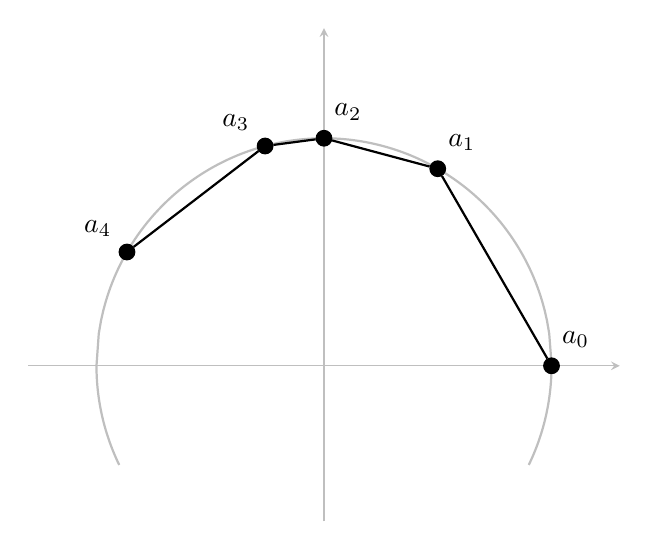
\begin{tikzpicture}
		\begin{axis}[
		xmin=-1.3,xmax=1.3,
		ymin=-0.5,ymax=1.3,
		ytick={-1,1},
		xtick={-1,1},
		xticklabels={},
		yticklabels={},
		axis lines=middle,
		axis line style=lightgray,
		width=0.75\textwidth,
		axis equal,
		]
		
		\addplot[lightgray,style=thick,-] expression[domain=-1:1,samples=200]{sqrt(1-x^2)}; 
		\addplot[lightgray,style=thick,-] expression[domain=0.9:1,samples=200]{-sqrt(1-x^2)};
		\addplot[lightgray,style=thick,-] expression[domain=-1:-0.9,samples=200]{-sqrt(1-x^2)};
		
		
		\node[label={85:{$a_0$}},color=black,draw=black,circle,fill,inner sep=2pt] at (axis cs:1,0) (A) {}; 
		\node[label={85:{$a_1$}},color=black,draw=black,circle,fill,inner sep=2pt] at (axis cs:0.5,0.866025) (B) {}; 
		\node[label={85:{$a_2$}},color=black,draw=black,circle,fill,inner sep=2pt] at (axis cs:0,1) (C) {}; 
		\node[label={135:{$a_3$}},color=black,draw=black,circle,fill,inner sep=2pt] at (axis cs:-0.258819,0.965926) (D) {};
		\node[label={135:{$a_4$}},color=black,draw=black,circle,fill,inner sep=2pt] at (axis cs:-0.866025,0.5) (E) {}; 
		
		\draw[black, thick] (A) -- (B) -- (C) -- (D) -- (E);
		
		\end{axis}
		\end{tikzpicture}
	\end{center}
	\caption{Given a list of points $P = a_0, \dotsc, a_n$ in counterclockwise order, we define $\len(P)$ to be the sum of the euclidean distatnces between $a_{i-1}$ to $a_i$ for all $i = 1, \dotsc, n$. In the picture above, this is the total length of the line segments between the points.}  \label{circle-length-of-list}
\end{figure}

Given a point $a \in S^1$, a \emph{partition of the arclength from $(1,0)$ to $a$} is a finite list of points $a_0, \dotsc, a_n$ in counterclockwise order with $a_0 = (1,0)$ and $a_n = a$. We then define
\[ \arclen(a) = \sup \{ \len(P) : P \text{ is a partition of the arclength from } (1,0) \text{ to } a \}. \] 
Notice that $\arclen(1,0) = 0$ and $\arclen(a) \geq 0$ for all $a$. \Cref{arclength-finite} shows that $\arclen(a)$ is a  finite real number, so we have defined a function $\arclen : S^1 \to \R$. 

\begin{lemma} \label{arclength-finite}
	For any $a \in S^1$, we have $\arclen(a) \leq 8$. 
\end{lemma}

\begin{proof}
	Let $(1, 0) = a_0, \dotsc, a_n$ be a list in counterclockwise order. It is sufficient to show that 
	\begin{equation} \label{inscribed-polygon-perimeter} |a_0 - a_1|_2 + \dotsb + |a_{n-1} - a_n| + |a_n - a_0| \leq 8. \end{equation}
	Geometrically, this assertion says that the perimeter of any polygon inscribed inside the unit circle is at most 8. By the triangle inequality, inserting points into the list $a_0, \dotsc, a_n$ increases the left hand side of inequality \ref{inscribed-polygon-perimeter}. So, to prove \cref{inscribed-polygon-perimeter}, we can assume without loss of generality that the four points $(\pm 1, 0), (0, \pm 1)$ all show up in the list $a_0, \dotsc, a_n$. If $a_k = (0,1)$, by symmetry it is sufficient to show that 
	\[ |a_0 - a_1| + \dotsb + |a_{k-1} - a_k| \leq 2. \]
	This follows from the triangle inequality. See \cref{arclength-finite-picture}. 
	\begin{figure}[ht]
		\begin{center}
			\begin{tikzpicture}
			\begin{axis}[
			xmin=-0.2,xmax=1.1,
			ymin=-0.2,ymax=1.1,
			ytick={-1,1},
			xtick={-1,1},
			xticklabels={},
			yticklabels={},
			axis lines=middle,
			axis line style=lightgray,
			width=0.75\textwidth,
			axis equal
			]
			
			\addplot[lightgray,style=thick,-] expression[domain=-0.1:1,samples=200]{sqrt(1-x^2)}; 
			\addplot[lightgray,style=thick,-] expression[domain=0.9:1,samples=200]{-sqrt(1-x^2)};
			
			\node[label={45:{$a_0$}},color=black,draw=black,circle,fill,inner sep=2pt] at (axis cs:1,0) (A) {}; 
			\node[label={85:{$a_1$}},color=black,draw=black,circle,fill,inner sep=2pt] at (axis cs:0.5,0.866025) (B) {}; 
			\node[label={85:{$a_2$}},color=black,draw=black,circle,fill,inner sep=2pt] at (axis cs:0.258819,0.965926) (C) {};
			\node[label={135:{$a_3$}},color=black,draw=black,circle,fill,inner sep=2pt] at (axis cs:0,1) (D) {}; 
			
			
			\node[inner sep=0pt] at (axis cs:1,0.866025) (E) {}; 
			\node[inner sep=0pt] at (axis cs:0.5,0.965926) (F) {}; 
			\node[inner sep=0pt] at (axis cs:0.258819,1) (G) {};
			
			\draw[black, thick] (A) -- (B) -- (C) -- (D);
			
			\draw[black, dashed] (A) -- (E) -- (B) -- (F) -- (C) -- (G) -- (D);
			
			\end{axis}
			\end{tikzpicture}
		\end{center}
		\caption{If $(1,0) = a_0, \dotsc, a_k= (0,1)$ is list in counterclockwise order, then the sum of the euclidean distances is the total length of the black lines drawn above. This is at most the sum of the lengths of the vertical and horizontal dashed lines, by the triangle inequality. Since the total vertical length of the dashed lines is 1 and so is the total horizontal length, we conclude that the sum of the euclidean distances is at most $2$.}  \label{arclength-finite-picture}
	\end{figure}
\end{proof}

\begin{lemma} \label{arclen-strictly-increasing}
	$\arclen$ is an injective function. In fact, if $b$ is counterclockwise of $a$ and $b \neq a$, then $\arclen(b) > \arclen(a)$. 
\end{lemma}

\begin{proof}
	Suppose $P$ is a partition of the arclength from $(1,0)$ to $a$. Tacking on $b$ yields a new list $P'$ that is a partition of the arclength from $(1,0)$ to $b$, so
	\[ \len(P) + |b-a|_2 = \len(P') \leq \arclen(b). \]
	Taking the supremum over all $P \in \mathscr{P}(a)$ shows that 
	\[ \arclen(a) + |b-a|_2 \leq \arclen(b). \]
	In particular, $\arclen(a) < \arclen(b)$. 
\end{proof}

\begin{remark} \label{taxicab-norm}
	In the following proof, we will use the \emph{$L^1$ norm} or the \emph{taxicab norm} on $\R^2$. It is defined by 
	\[ |(x,y)|_1 = |x| + |y|. \]
	Observe that for any $a  \in \R^2$,  
	\[ |a|_2 \leq |a|_1 \leq \sqrt{2}|a|_2. \]
	Moreover, if $a$ and $b$ are two points in $\R^2$ in the same quadrant (where points on coordinate axes are considered to be in all quadrants they are contiguous to), then 
	\[ |a|_1 + |b|_1 = |a+b|_1. \]
\end{remark}

\begin{lemma} \label{arclen-continuous}
	$\arclen$ is continuous away from $(1,0)$. 
\end{lemma}

\begin{proof}
	Suppose $a, b \neq (1,0)$ are in the same quadrant of the plane (where points on the axes are considered to be in both quadrants they are contiguous to), and that $b$ is  counterclockwise of $a$. Fix $\epsilon > 0$. Let $P$ be a partition of the arclength from $(1,0)$ to $a$ such that $\arclen(a) - \len(P) \leq \epsilon$. 
	
	Let $Q$ be a partition of the arclength from $(1,0)$ to $b$ such that $\arclen(b) - \len(Q) \leq \epsilon$. If $Q'$ is the partition of the arclength from $(1,0)$ to $b$ obtained by merging $P$ and $Q$, observe that $\len(Q) \leq \len(Q')$, so $\arclen(b) - \len(Q') < \epsilon$ also. Thus we can replace $Q$ with $Q'$ in order to assume that $P$ is a sublist of $Q$. 
	
	Let $R = a_0, \dotsc, a_m$ be the sublist of $Q$ starting from $a_0 = a$ and ending with $a_m = b$, so that $\len(P) + \len(R) = \len(Q)$. Then 
	\[ \len(R) \leq |a_0 - a_1|_1 + \dotsb + |a_{m-1} - a_m|_1 = |b-a|_1 \leq \sqrt{2}|b-a|_2, \]
	using \cref{taxicab-norm}. For the equality in the middle, we have used the fact that since $a$ and $b$ are in the same quadrant, all of the points $a_0 - a_1, a_1 - a_2, \dotsc, a_{m-1} - a_m$ are also in the same quadrant. Thus
	\[ 0 \leq \arclen(b) - \arclen(a) \leq \len(Q) - \len(P) + 2\epsilon = \len(R) + 2\epsilon \leq \sqrt{2}|b-a|_2 + 2\epsilon. \]
	Letting $\epsilon \to 0^+$, we find that 
	\[ 0 \leq \arclen(b) - \arclen(a) \leq \sqrt{2}|b-a|_2, \]
	which proves that $\arclen$ is continuous. 
\end{proof}

\section{Definition of \texorpdfstring{$\pi$}{pi}}

\begin{definition}
	We define $\pi$ to be the unique positive real number with  the property that 
	\[ 2\pi = \sup \arclen(S^1). \]
	We know from \cref{arclength-finite} that this supremum is finite. 
\end{definition}

\begin{lemma}
	$\arclen(S^1) = [0, 2\pi)$. 
\end{lemma}

\begin{proof}
	Let $U = S^1 \setminus \{(1,0)\}$. Then $U$ is connected and $\arclen|_U$ is continuous, so $\arclen(U)$ is an interval. It is clear that $\inf \arclen(U) = 0$, and we know that $\arclen(1,0) = 0$, so $0 \in \arclen(S^1)$. Now \[ 2\pi = \sup \arclen(S^1) = \sup \arclen(U). \]
	If there existed $a \in S^1$ such that $\arclen(a) = 2\pi$, then we could choose a point $b$ which is counterclockwise of $a$ and $b \neq a$. Then $\arclen(b) > \arclen(a) = 2\pi$ by \cref{arclen-strictly-increasing}, contradicting the definition of $2\pi$ as a supremum. Thus $2\pi$ is not in the image of $\arclen$, proving the lemma.  
\end{proof}

\begin{exercise}
	Show that $\pi = \arclen(-1,0)$. 
\end{exercise}

\section{Sine and cosine}

We have seen that $\arclen$ is a bijection $S^1 \to [0, 2\pi)$. We can now define sine and cosine in terms of the inverse function $\arclen^{-1} : [0, 2\pi) \to S^1$.  

\begin{definition}
	For $\theta \in [0, 2\pi)$, we define the \emph{cosine} and \emph{sine} of $\theta$, denoted $\cos(\theta)$ and $\sin(\theta)$, to be the $x$- and $y$-coordinates of $\arclen^{-1}(\theta)$, respectively. In other words,
	\[ \arclen^{-1}(\theta) = (\cos(\theta), \sin(\theta)). \]
	Then, for any $\theta \in \R$, there exists a unique $\theta' \in [0, 2\pi)$ such that $\theta = \theta' + 2\pi k$ for some integer $k$, and we define $\cos(\theta) = \cos(\theta')$ and $\sin(\theta) = \sin(\theta')$. 
\end{definition}

% TODO: Continuity

% TODO: sin x / x

% TODO: angle sum formula for sine

% TODO: cos(x) = sin(pi/2 - x)
	\chapter{Selected solutions}
\includecollection{sols}
	
	\printbibliography
	
	\printindex
	
\end{document}